\documentclass[twoside]{book}

% Packages required by doxygen
\usepackage{fixltx2e}
\usepackage{calc}
\usepackage{doxygen}
\usepackage{graphicx}
\usepackage[utf8]{inputenc}
\usepackage{makeidx}
\usepackage{multicol}
\usepackage{multirow}
\PassOptionsToPackage{warn}{textcomp}
\usepackage{textcomp}
\usepackage[nointegrals]{wasysym}
\usepackage[table]{xcolor}

% NLS support packages
\usepackage[english]{babel}
\usepackage[T1]{fontenc}

% Font selection
\usepackage[T1]{fontenc}
\usepackage{mathptmx}
\usepackage[scaled=1.0]{helvet}
\usepackage{courier}
\usepackage{amssymb}
\usepackage{sectsty}
\renewcommand{\familydefault}{\sfdefault}
\allsectionsfont{%
  \fontseries{bc}\selectfont%
  \color{darkgray}%
}
\renewcommand{\DoxyLabelFont}{%
  \fontseries{bc}\selectfont%
  \color{darkgray}%
}
\newcommand{\+}{\discretionary{\mbox{\scriptsize$\hookleftarrow$}}{}{}}

% Page & text layout
\usepackage{geometry}
\geometry{%
  a4paper,%
  top=2.5cm,%
  bottom=2.5cm,%
  left=2.5cm,%
  right=2.5cm%
}
\tolerance=750
\hfuzz=15pt
\hbadness=750
\setlength{\emergencystretch}{15pt}
\setlength{\parindent}{0cm}
\setlength{\parskip}{0.2cm}
\makeatletter
\renewcommand{\paragraph}{%
  \@startsection{paragraph}{4}{0ex}{-1.0ex}{1.0ex}{%
    \normalfont\normalsize\bfseries\SS@parafont%
  }%
}
\renewcommand{\subparagraph}{%
  \@startsection{subparagraph}{5}{0ex}{-1.0ex}{1.0ex}{%
    \normalfont\normalsize\bfseries\SS@subparafont%
  }%
}
\makeatother

% Headers & footers
\usepackage{fancyhdr}
\pagestyle{fancyplain}
\fancyhead[LE]{\fancyplain{}{\bfseries\thepage}}
\fancyhead[CE]{\fancyplain{}{}}
\fancyhead[RE]{\fancyplain{}{\bfseries\leftmark}}
\fancyhead[LO]{\fancyplain{}{\bfseries\rightmark}}
\fancyhead[CO]{\fancyplain{}{}}
\fancyhead[RO]{\fancyplain{}{\bfseries\thepage}}
\fancyfoot[LE]{\fancyplain{}{}}
\fancyfoot[CE]{\fancyplain{}{}}
\fancyfoot[RE]{\fancyplain{}{\bfseries\scriptsize Generert Thu Sep 4 2014 13\+:43\+:48 for Scintilab av Doxygen }}
\fancyfoot[LO]{\fancyplain{}{\bfseries\scriptsize Generert Thu Sep 4 2014 13\+:43\+:48 for Scintilab av Doxygen }}
\fancyfoot[CO]{\fancyplain{}{}}
\fancyfoot[RO]{\fancyplain{}{}}
\renewcommand{\footrulewidth}{0.4pt}
\renewcommand{\chaptermark}[1]{%
  \markboth{#1}{}%
}
\renewcommand{\sectionmark}[1]{%
  \markright{\thesection\ #1}%
}

% Indices & bibliography
\usepackage{natbib}
\usepackage[titles]{tocloft}
\setcounter{tocdepth}{3}
\setcounter{secnumdepth}{5}
\makeindex

% Hyperlinks (required, but should be loaded last)
\usepackage{ifpdf}
\ifpdf
  \usepackage[pdftex,pagebackref=true]{hyperref}
\else
  \usepackage[ps2pdf,pagebackref=true]{hyperref}
\fi
\hypersetup{%
  colorlinks=true,%
  linkcolor=blue,%
  citecolor=blue,%
  unicode%
}

% Custom commands
\newcommand{\clearemptydoublepage}{%
  \newpage{\pagestyle{empty}\cleardoublepage}%
}


%===== C O N T E N T S =====

\begin{document}

% Titlepage & ToC
\hypersetup{pageanchor=false,
             bookmarks=true,
             bookmarksnumbered=true,
             pdfencoding=unicode
            }
\pagenumbering{roman}
\begin{titlepage}
\vspace*{7cm}
\begin{center}%
{\Large Scintilab }\\
\vspace*{1cm}
{\large Generert av Doxygen 1.8.7}\\
\vspace*{0.5cm}
{\small Thu Sep 4 2014 13:43:48}\\
\end{center}
\end{titlepage}
\clearemptydoublepage
\tableofcontents
\clearemptydoublepage
\pagenumbering{arabic}
\hypersetup{pageanchor=true}

%--- Begin generated contents ---
\chapter{Navneromsindeks}
\section{Navneromsliste}
Her er en liste over alle navnerom med korte beskrivelser\+:\begin{DoxyCompactList}
\item\contentsline{section}{\hyperlink{namespace_scintilab}{Scintilab} }{\pageref{namespace_scintilab}}{}
\end{DoxyCompactList}

\chapter{Hierarkisk indeks}
\section{Klassehierarki}
Denne arvelisten er grovsortert alfabetisk (ikke nødvendigvis korrekt)\+:\begin{DoxyCompactList}
\item \contentsline{section}{Scintilab.\+Beaker}{\pageref{class_scintilab_1_1_beaker}}{}
\item \contentsline{section}{Scintilab.\+Beaker\+Info}{\pageref{class_scintilab_1_1_beaker_info}}{}
\item \contentsline{section}{Scintilab.\+Config}{\pageref{class_scintilab_1_1_config}}{}
\item \contentsline{section}{Scintilab.\+Detector}{\pageref{class_scintilab_1_1_detector}}{}
\item Form\begin{DoxyCompactList}
\item \contentsline{section}{Scintilab.\+Form\+Barcode\+Sample}{\pageref{class_scintilab_1_1_form_barcode_sample}}{}
\item \contentsline{section}{Scintilab.\+Form\+Barcode\+Sample\+Wizard}{\pageref{class_scintilab_1_1_form_barcode_sample_wizard}}{}
\item \contentsline{section}{Scintilab.\+Form\+Create\+Geom\+Cal\+Q\+A}{\pageref{class_scintilab_1_1_form_create_geom_cal_q_a}}{}
\item \contentsline{section}{Scintilab.\+Form\+Edit\+Geom\+Cal\+Q\+A}{\pageref{class_scintilab_1_1_form_edit_geom_cal_q_a}}{}
\item \contentsline{section}{Scintilab.\+Form\+Input\+Name}{\pageref{class_scintilab_1_1_form_input_name}}{}
\item \contentsline{section}{Scintilab.\+Form\+Job\+Report}{\pageref{class_scintilab_1_1_form_job_report}}{}
\item \contentsline{section}{Scintilab.\+Form\+Login}{\pageref{class_scintilab_1_1_form_login}}{}
\item \contentsline{section}{Scintilab.\+Form\+Main}{\pageref{class_scintilab_1_1_form_main}}{}
\item \contentsline{section}{Scintilab.\+Form\+Quick\+View}{\pageref{class_scintilab_1_1_form_quick_view}}{}
\end{DoxyCompactList}
\item \contentsline{section}{Scintilab.\+Job\+Params}{\pageref{class_scintilab_1_1_job_params}}{}
\item \contentsline{section}{Scintilab.\+Media}{\pageref{class_scintilab_1_1_media}}{}
\item Print\+Document\begin{DoxyCompactList}
\item \contentsline{section}{Multipad\+Print\+Document}{\pageref{class_multipad_print_document}}{}
\end{DoxyCompactList}
\item \contentsline{section}{Scintilab.\+Q\+A\+Beaker}{\pageref{class_scintilab_1_1_q_a_beaker}}{}
\item \contentsline{section}{Scintilab.\+Selection\+Info}{\pageref{class_scintilab_1_1_selection_info}}{}
\item \contentsline{section}{Scintilab.\+System\+Parameters}{\pageref{class_scintilab_1_1_system_parameters}}{}
\item \contentsline{section}{Scintilab.\+Utils}{\pageref{class_scintilab_1_1_utils}}{}
\end{DoxyCompactList}

\chapter{Klasseindeks}
\section{Klasseliste}
Her er klasser, struct'er, unioner og interface'er med korte beskrivelser\+:\begin{DoxyCompactList}
\item\contentsline{section}{\hyperlink{class_scintilab_1_1_beaker}{Scintilab.\+Beaker} \\*Datastruktur for begere }{\pageref{class_scintilab_1_1_beaker}}{}
\item\contentsline{section}{\hyperlink{class_scintilab_1_1_beaker_info}{Scintilab.\+Beaker\+Info} \\*Datastruktur for beger/calibrering/\+Q\+A kombinasjon }{\pageref{class_scintilab_1_1_beaker_info}}{}
\item\contentsline{section}{\hyperlink{class_scintilab_1_1_config}{Scintilab.\+Config} }{\pageref{class_scintilab_1_1_config}}{}
\item\contentsline{section}{\hyperlink{class_scintilab_1_1_detector}{Scintilab.\+Detector} \\*Datastruktur for detektor }{\pageref{class_scintilab_1_1_detector}}{}
\item\contentsline{section}{\hyperlink{class_scintilab_1_1_form_barcode_sample}{Scintilab.\+Form\+Barcode\+Sample} \\*Klasse for innlesing av strekkode }{\pageref{class_scintilab_1_1_form_barcode_sample}}{}
\item\contentsline{section}{\hyperlink{class_scintilab_1_1_form_barcode_sample_wizard}{Scintilab.\+Form\+Barcode\+Sample\+Wizard} \\*Klasse for innlesing av strekkoder }{\pageref{class_scintilab_1_1_form_barcode_sample_wizard}}{}
\item\contentsline{section}{\hyperlink{class_scintilab_1_1_form_create_geom_cal_q_a}{Scintilab.\+Form\+Create\+Geom\+Cal\+Q\+A} \\*Klasse for oppretting av Beger/\+Calibrasjon/\+Q\+A kombinasjon }{\pageref{class_scintilab_1_1_form_create_geom_cal_q_a}}{}
\item\contentsline{section}{\hyperlink{class_scintilab_1_1_form_edit_geom_cal_q_a}{Scintilab.\+Form\+Edit\+Geom\+Cal\+Q\+A} \\*Klasse for editering av Beger/\+Calibrasjon/\+Q\+A kombinasjon }{\pageref{class_scintilab_1_1_form_edit_geom_cal_q_a}}{}
\item\contentsline{section}{\hyperlink{class_scintilab_1_1_form_input_name}{Scintilab.\+Form\+Input\+Name} \\*Klasse for innlesing av et generisk navn fra bruker }{\pageref{class_scintilab_1_1_form_input_name}}{}
\item\contentsline{section}{\hyperlink{class_scintilab_1_1_form_job_report}{Scintilab.\+Form\+Job\+Report} \\*Klasse for visning av jobb rapport }{\pageref{class_scintilab_1_1_form_job_report}}{}
\item\contentsline{section}{\hyperlink{class_scintilab_1_1_form_login}{Scintilab.\+Form\+Login} \\*Klasse for innlogging }{\pageref{class_scintilab_1_1_form_login}}{}
\item\contentsline{section}{\hyperlink{class_scintilab_1_1_form_main}{Scintilab.\+Form\+Main} \\*Hovedklasse for \hyperlink{namespace_scintilab}{Scintilab} }{\pageref{class_scintilab_1_1_form_main}}{}
\item\contentsline{section}{\hyperlink{class_scintilab_1_1_form_quick_view}{Scintilab.\+Form\+Quick\+View} \\*Klasse for generisk visning av tekst }{\pageref{class_scintilab_1_1_form_quick_view}}{}
\item\contentsline{section}{\hyperlink{class_scintilab_1_1_job_params}{Scintilab.\+Job\+Params} \\*Datastruktur for jobb parametere }{\pageref{class_scintilab_1_1_job_params}}{}
\item\contentsline{section}{\hyperlink{class_scintilab_1_1_media}{Scintilab.\+Media} }{\pageref{class_scintilab_1_1_media}}{}
\item\contentsline{section}{\hyperlink{class_multipad_print_document}{Multipad\+Print\+Document} }{\pageref{class_multipad_print_document}}{}
\item\contentsline{section}{\hyperlink{class_scintilab_1_1_q_a_beaker}{Scintilab.\+Q\+A\+Beaker} \\*Datastruktur for Q\+A-\/begere }{\pageref{class_scintilab_1_1_q_a_beaker}}{}
\item\contentsline{section}{\hyperlink{class_scintilab_1_1_selection_info}{Scintilab.\+Selection\+Info} \\*Klasse for parametere valgt av bruker gjennom grensesnitt }{\pageref{class_scintilab_1_1_selection_info}}{}
\item\contentsline{section}{\hyperlink{class_scintilab_1_1_system_parameters}{Scintilab.\+System\+Parameters} \\*Datastruktur for systemparametere }{\pageref{class_scintilab_1_1_system_parameters}}{}
\item\contentsline{section}{\hyperlink{class_scintilab_1_1_utils}{Scintilab.\+Utils} }{\pageref{class_scintilab_1_1_utils}}{}
\end{DoxyCompactList}

\chapter{Filindeks}
\section{Fil-\/liste}
Her er en liste over alle filer med korte beskrivelser\+:\begin{DoxyCompactList}
\item\contentsline{section}{\hyperlink{_config_8cs}{Config.\+cs} }{\pageref{_config_8cs}}{}
\item\contentsline{section}{\hyperlink{_form_barcode_sample_8cs}{Form\+Barcode\+Sample.\+cs} }{\pageref{_form_barcode_sample_8cs}}{}
\item\contentsline{section}{\hyperlink{_form_barcode_sample_wizard_8cs}{Form\+Barcode\+Sample\+Wizard.\+cs} }{\pageref{_form_barcode_sample_wizard_8cs}}{}
\item\contentsline{section}{\hyperlink{_form_create_geom_cal_q_a_8cs}{Form\+Create\+Geom\+Cal\+Q\+A.\+cs} }{\pageref{_form_create_geom_cal_q_a_8cs}}{}
\item\contentsline{section}{\hyperlink{_form_edit_geom_cal_q_a_8cs}{Form\+Edit\+Geom\+Cal\+Q\+A.\+cs} }{\pageref{_form_edit_geom_cal_q_a_8cs}}{}
\item\contentsline{section}{\hyperlink{_form_input_name_8cs}{Form\+Input\+Name.\+cs} }{\pageref{_form_input_name_8cs}}{}
\item\contentsline{section}{\hyperlink{_form_job_report_8cs}{Form\+Job\+Report.\+cs} }{\pageref{_form_job_report_8cs}}{}
\item\contentsline{section}{\hyperlink{_form_login_8cs}{Form\+Login.\+cs} }{\pageref{_form_login_8cs}}{}
\item\contentsline{section}{\hyperlink{_form_main_8cs}{Form\+Main.\+cs} }{\pageref{_form_main_8cs}}{}
\item\contentsline{section}{\hyperlink{_form_quick_view_8cs}{Form\+Quick\+View.\+cs} }{\pageref{_form_quick_view_8cs}}{}
\item\contentsline{section}{\hyperlink{_multipad_print_document_8cs}{Multipad\+Print\+Document.\+cs} }{\pageref{_multipad_print_document_8cs}}{}
\item\contentsline{section}{\hyperlink{_program_8cs}{Program.\+cs} }{\pageref{_program_8cs}}{}
\item\contentsline{section}{\hyperlink{_types_8cs}{Types.\+cs} }{\pageref{_types_8cs}}{}
\item\contentsline{section}{\hyperlink{_utils_8cs}{Utils.\+cs} }{\pageref{_utils_8cs}}{}
\end{DoxyCompactList}

\chapter{Navneromsdokumentasjon}
\hypertarget{namespace_scintilab}{\section{Package Scintilab}
\label{namespace_scintilab}\index{Scintilab@{Scintilab}}
}
\subsection*{Klasser}
\begin{DoxyCompactItemize}
\item 
class \hyperlink{class_scintilab_1_1_beaker}{Beaker}
\begin{DoxyCompactList}\small\item\em Datastruktur for begere. \end{DoxyCompactList}\item 
class \hyperlink{class_scintilab_1_1_beaker_info}{Beaker\+Info}
\begin{DoxyCompactList}\small\item\em Datastruktur for beger/calibrering/\+Q\+A kombinasjon. \end{DoxyCompactList}\item 
class \hyperlink{class_scintilab_1_1_config}{Config}
\item 
class \hyperlink{class_scintilab_1_1_detector}{Detector}
\begin{DoxyCompactList}\small\item\em Datastruktur for detektor. \end{DoxyCompactList}\item 
class \hyperlink{class_scintilab_1_1_form_barcode_sample}{Form\+Barcode\+Sample}
\begin{DoxyCompactList}\small\item\em Klasse for innlesing av strekkode. \end{DoxyCompactList}\item 
class \hyperlink{class_scintilab_1_1_form_barcode_sample_wizard}{Form\+Barcode\+Sample\+Wizard}
\begin{DoxyCompactList}\small\item\em Klasse for innlesing av strekkoder. \end{DoxyCompactList}\item 
class \hyperlink{class_scintilab_1_1_form_create_geom_cal_q_a}{Form\+Create\+Geom\+Cal\+Q\+A}
\begin{DoxyCompactList}\small\item\em Klasse for oppretting av Beger/\+Calibrasjon/\+Q\+A kombinasjon. \end{DoxyCompactList}\item 
class \hyperlink{class_scintilab_1_1_form_edit_geom_cal_q_a}{Form\+Edit\+Geom\+Cal\+Q\+A}
\begin{DoxyCompactList}\small\item\em Klasse for editering av Beger/\+Calibrasjon/\+Q\+A kombinasjon. \end{DoxyCompactList}\item 
class \hyperlink{class_scintilab_1_1_form_input_name}{Form\+Input\+Name}
\begin{DoxyCompactList}\small\item\em Klasse for innlesing av et generisk navn fra bruker. \end{DoxyCompactList}\item 
class \hyperlink{class_scintilab_1_1_form_job_report}{Form\+Job\+Report}
\begin{DoxyCompactList}\small\item\em Klasse for visning av jobb rapport. \end{DoxyCompactList}\item 
class \hyperlink{class_scintilab_1_1_form_login}{Form\+Login}
\begin{DoxyCompactList}\small\item\em Klasse for innlogging. \end{DoxyCompactList}\item 
class \hyperlink{class_scintilab_1_1_form_main}{Form\+Main}
\begin{DoxyCompactList}\small\item\em Hovedklasse for \hyperlink{namespace_scintilab}{Scintilab}. \end{DoxyCompactList}\item 
class \hyperlink{class_scintilab_1_1_form_quick_view}{Form\+Quick\+View}
\begin{DoxyCompactList}\small\item\em Klasse for generisk visning av tekst. \end{DoxyCompactList}\item 
class \hyperlink{class_scintilab_1_1_job_params}{Job\+Params}
\begin{DoxyCompactList}\small\item\em Datastruktur for jobb parametere. \end{DoxyCompactList}\item 
class \hyperlink{class_scintilab_1_1_media}{Media}
\item 
class {\bfseries Program}
\item 
class \hyperlink{class_scintilab_1_1_q_a_beaker}{Q\+A\+Beaker}
\begin{DoxyCompactList}\small\item\em Datastruktur for Q\+A-\/begere. \end{DoxyCompactList}\item 
class \hyperlink{class_scintilab_1_1_selection_info}{Selection\+Info}
\begin{DoxyCompactList}\small\item\em Klasse for parametere valgt av bruker gjennom grensesnitt. \end{DoxyCompactList}\item 
class \hyperlink{class_scintilab_1_1_system_parameters}{System\+Parameters}
\begin{DoxyCompactList}\small\item\em Datastruktur for systemparametere. \end{DoxyCompactList}\item 
class \hyperlink{class_scintilab_1_1_utils}{Utils}
\end{DoxyCompactItemize}

\chapter{Klassedokumentasjon}
\hypertarget{class_scintilab_1_1_beaker}{\section{Scintilab.\+Beaker Klasse Referanse}
\label{class_scintilab_1_1_beaker}\index{Scintilab.\+Beaker@{Scintilab.\+Beaker}}
}


Datastruktur for begere.  


\subsection*{Public attributter}
\begin{DoxyCompactItemize}
\item 
string \hyperlink{class_scintilab_1_1_beaker_acb97eb3b7c1a9448162a6f526152713c}{Name}
\item 
string \hyperlink{class_scintilab_1_1_beaker_a54c85016c0711130d2b977db5004d694}{Manufacturer}
\item 
bool \hyperlink{class_scintilab_1_1_beaker_a5e26e17ccd65399bba732ebb21050f94}{In\+Use}
\end{DoxyCompactItemize}


\subsection{Detaljert beskrivelse}
Datastruktur for begere. 

Definisjon på linje 26 i filen Types.\+cs.



\subsection{Medlemsdata-\/dokumentasjon}
\hypertarget{class_scintilab_1_1_beaker_a5e26e17ccd65399bba732ebb21050f94}{\index{Scintilab\+::\+Beaker@{Scintilab\+::\+Beaker}!In\+Use@{In\+Use}}
\index{In\+Use@{In\+Use}!Scintilab\+::\+Beaker@{Scintilab\+::\+Beaker}}
\subsubsection[{In\+Use}]{\setlength{\rightskip}{0pt plus 5cm}bool Scintilab.\+Beaker.\+In\+Use}}\label{class_scintilab_1_1_beaker_a5e26e17ccd65399bba732ebb21050f94}


Definisjon på linje 30 i filen Types.\+cs.

\hypertarget{class_scintilab_1_1_beaker_a54c85016c0711130d2b977db5004d694}{\index{Scintilab\+::\+Beaker@{Scintilab\+::\+Beaker}!Manufacturer@{Manufacturer}}
\index{Manufacturer@{Manufacturer}!Scintilab\+::\+Beaker@{Scintilab\+::\+Beaker}}
\subsubsection[{Manufacturer}]{\setlength{\rightskip}{0pt plus 5cm}string Scintilab.\+Beaker.\+Manufacturer}}\label{class_scintilab_1_1_beaker_a54c85016c0711130d2b977db5004d694}


Definisjon på linje 29 i filen Types.\+cs.

\hypertarget{class_scintilab_1_1_beaker_acb97eb3b7c1a9448162a6f526152713c}{\index{Scintilab\+::\+Beaker@{Scintilab\+::\+Beaker}!Name@{Name}}
\index{Name@{Name}!Scintilab\+::\+Beaker@{Scintilab\+::\+Beaker}}
\subsubsection[{Name}]{\setlength{\rightskip}{0pt plus 5cm}string Scintilab.\+Beaker.\+Name}}\label{class_scintilab_1_1_beaker_acb97eb3b7c1a9448162a6f526152713c}


Definisjon på linje 28 i filen Types.\+cs.



Dokumentasjonen for denne klasse ble generert fra følgende fil\+:\begin{DoxyCompactItemize}
\item 
\hyperlink{_types_8cs}{Types.\+cs}\end{DoxyCompactItemize}

\hypertarget{class_scintilab_1_1_beaker_info}{\section{Scintilab.\+Beaker\+Info Klasse Referanse}
\label{class_scintilab_1_1_beaker_info}\index{Scintilab.\+Beaker\+Info@{Scintilab.\+Beaker\+Info}}
}


Datastruktur for beger/calibrering/\+Q\+A kombinasjon.  


\subsection*{Public attributter}
\begin{DoxyCompactItemize}
\item 
string \hyperlink{class_scintilab_1_1_beaker_info_ad64e0fe748757fb68caf76b4809bef13}{Beaker\+Name}
\item 
string \hyperlink{class_scintilab_1_1_beaker_info_a978205fb02070c6986658d7dd4d906fa}{Calibration\+File}
\item 
string \hyperlink{class_scintilab_1_1_beaker_info_a77fc3aac52eb159c41750b306033e06e}{Q\+A\+Name}
\end{DoxyCompactItemize}


\subsection{Detaljert beskrivelse}
Datastruktur for beger/calibrering/\+Q\+A kombinasjon. 

Definisjon på linje 51 i filen Types.\+cs.



\subsection{Medlemsdata-\/dokumentasjon}
\hypertarget{class_scintilab_1_1_beaker_info_ad64e0fe748757fb68caf76b4809bef13}{\index{Scintilab\+::\+Beaker\+Info@{Scintilab\+::\+Beaker\+Info}!Beaker\+Name@{Beaker\+Name}}
\index{Beaker\+Name@{Beaker\+Name}!Scintilab\+::\+Beaker\+Info@{Scintilab\+::\+Beaker\+Info}}
\subsubsection[{Beaker\+Name}]{\setlength{\rightskip}{0pt plus 5cm}string Scintilab.\+Beaker\+Info.\+Beaker\+Name}}\label{class_scintilab_1_1_beaker_info_ad64e0fe748757fb68caf76b4809bef13}


Definisjon på linje 53 i filen Types.\+cs.

\hypertarget{class_scintilab_1_1_beaker_info_a978205fb02070c6986658d7dd4d906fa}{\index{Scintilab\+::\+Beaker\+Info@{Scintilab\+::\+Beaker\+Info}!Calibration\+File@{Calibration\+File}}
\index{Calibration\+File@{Calibration\+File}!Scintilab\+::\+Beaker\+Info@{Scintilab\+::\+Beaker\+Info}}
\subsubsection[{Calibration\+File}]{\setlength{\rightskip}{0pt plus 5cm}string Scintilab.\+Beaker\+Info.\+Calibration\+File}}\label{class_scintilab_1_1_beaker_info_a978205fb02070c6986658d7dd4d906fa}


Definisjon på linje 54 i filen Types.\+cs.

\hypertarget{class_scintilab_1_1_beaker_info_a77fc3aac52eb159c41750b306033e06e}{\index{Scintilab\+::\+Beaker\+Info@{Scintilab\+::\+Beaker\+Info}!Q\+A\+Name@{Q\+A\+Name}}
\index{Q\+A\+Name@{Q\+A\+Name}!Scintilab\+::\+Beaker\+Info@{Scintilab\+::\+Beaker\+Info}}
\subsubsection[{Q\+A\+Name}]{\setlength{\rightskip}{0pt plus 5cm}string Scintilab.\+Beaker\+Info.\+Q\+A\+Name}}\label{class_scintilab_1_1_beaker_info_a77fc3aac52eb159c41750b306033e06e}


Definisjon på linje 55 i filen Types.\+cs.



Dokumentasjonen for denne klasse ble generert fra følgende fil\+:\begin{DoxyCompactItemize}
\item 
\hyperlink{_types_8cs}{Types.\+cs}\end{DoxyCompactItemize}

\hypertarget{class_scintilab_1_1_config}{\section{Scintilab.\+Config Klasse Referanse}
\label{class_scintilab_1_1_config}\index{Scintilab.\+Config@{Scintilab.\+Config}}
}
\subsection*{Statiske public attributter}
\begin{DoxyCompactItemize}
\item 
static string \hyperlink{class_scintilab_1_1_config_a64f1560197ddefe3f0e43bd620dd72c8}{Scintilab\+Dir}
\item 
static string \hyperlink{class_scintilab_1_1_config_afdad0bcf0906fdd0e7f34b3400fa8809}{Bkg\+Dir}
\item 
static string \hyperlink{class_scintilab_1_1_config_a7254f3412dd5234d0691262a8b898fd7}{Lib\+Dir}
\item 
static string \hyperlink{class_scintilab_1_1_config_a8bb782f1eebd5ba14d686c57bc981298}{Cal\+Dir}
\item 
static string \hyperlink{class_scintilab_1_1_config_a281e06e21224c52ea875ca48a91285ac}{Template\+Dir}
\item 
static string \hyperlink{class_scintilab_1_1_config_a772b5a6dcac628889128d1a896b36658}{Archive\+Dir}
\item 
static string \hyperlink{class_scintilab_1_1_config_a0810c3c214672429b456af8f77e98632}{Job\+Dir}
\item 
static string \hyperlink{class_scintilab_1_1_config_a2cd246ee28cb2fbf3b3664e2de4e4a2f}{Temp\+Dir}
\item 
static string \hyperlink{class_scintilab_1_1_config_ae7e1416a22380f4b5825e0ab9e49ee43}{Q\+A\+Dir}
\item 
static string \hyperlink{class_scintilab_1_1_config_a1df46889d2f1072cbfcd82e85117b55f}{Exe\+Dir}
\item 
static string \hyperlink{class_scintilab_1_1_config_ac4f5562af1d1a600b566d6c8b8e51d35}{Templ\+Dir}
\item 
static string \hyperlink{class_scintilab_1_1_config_a08bd32b13d26a35e5888aa530b757fd8}{Sys\+File}
\item 
static string \hyperlink{class_scintilab_1_1_config_aceb97f9538b41c0176f8408f81cc07ef}{Det\+File}
\item 
static string \hyperlink{class_scintilab_1_1_config_a1a1585ef6037b90a42a2fd1b2bac9b9d}{Beaker\+File}
\item 
static string \hyperlink{class_scintilab_1_1_config_a732e164c0f203b6dfccd10dd3081289d}{Q\+A\+Beaker\+File}
\item 
static string \hyperlink{class_scintilab_1_1_config_a022e7110df1c42b1bfcfb167400a2dbf}{Default\+Bkg\+Q\+A\+F\+File}
\item 
static string \hyperlink{class_scintilab_1_1_config_a9650ecffaee93e2d86f2c635f963b6fb}{Default\+Ref\+Q\+A\+F\+File}
\item 
static string \hyperlink{class_scintilab_1_1_config_a46bec74f1139be16639b257d38580f22}{Username}
\end{DoxyCompactItemize}


\subsection{Detaljert beskrivelse}
Klasse for \hyperlink{namespace_scintilab}{Scintilab} configurasjon. Denne klassen inneholder kataloger og filnavn som brukes av \hyperlink{namespace_scintilab}{Scintilab}. 

Definisjon på linje 13 i filen Config.\+cs.



\subsection{Medlemsdata-\/dokumentasjon}
\hypertarget{class_scintilab_1_1_config_a772b5a6dcac628889128d1a896b36658}{\index{Scintilab\+::\+Config@{Scintilab\+::\+Config}!Archive\+Dir@{Archive\+Dir}}
\index{Archive\+Dir@{Archive\+Dir}!Scintilab\+::\+Config@{Scintilab\+::\+Config}}
\subsubsection[{Archive\+Dir}]{\setlength{\rightskip}{0pt plus 5cm}string Scintilab.\+Config.\+Archive\+Dir\hspace{0.3cm}{\ttfamily [static]}}}\label{class_scintilab_1_1_config_a772b5a6dcac628889128d1a896b36658}
Katalog for arkivet. (.C\+N\+F, .P\+A\+R og .R\+P\+T filer) 

Definisjon på linje 26 i filen Config.\+cs.

\hypertarget{class_scintilab_1_1_config_a1a1585ef6037b90a42a2fd1b2bac9b9d}{\index{Scintilab\+::\+Config@{Scintilab\+::\+Config}!Beaker\+File@{Beaker\+File}}
\index{Beaker\+File@{Beaker\+File}!Scintilab\+::\+Config@{Scintilab\+::\+Config}}
\subsubsection[{Beaker\+File}]{\setlength{\rightskip}{0pt plus 5cm}string Scintilab.\+Config.\+Beaker\+File\hspace{0.3cm}{\ttfamily [static]}}}\label{class_scintilab_1_1_config_a1a1585ef6037b90a42a2fd1b2bac9b9d}
Filbane til geometri-\/definisjoner B\+E\+A\+K\+E\+R\+S.\+X\+M\+L 

Definisjon på linje 42 i filen Config.\+cs.

\hypertarget{class_scintilab_1_1_config_afdad0bcf0906fdd0e7f34b3400fa8809}{\index{Scintilab\+::\+Config@{Scintilab\+::\+Config}!Bkg\+Dir@{Bkg\+Dir}}
\index{Bkg\+Dir@{Bkg\+Dir}!Scintilab\+::\+Config@{Scintilab\+::\+Config}}
\subsubsection[{Bkg\+Dir}]{\setlength{\rightskip}{0pt plus 5cm}string Scintilab.\+Config.\+Bkg\+Dir\hspace{0.3cm}{\ttfamily [static]}}}\label{class_scintilab_1_1_config_afdad0bcf0906fdd0e7f34b3400fa8809}
Katalog for .C\+N\+F bakgrunnsfiler 

Definisjon på linje 18 i filen Config.\+cs.

\hypertarget{class_scintilab_1_1_config_a8bb782f1eebd5ba14d686c57bc981298}{\index{Scintilab\+::\+Config@{Scintilab\+::\+Config}!Cal\+Dir@{Cal\+Dir}}
\index{Cal\+Dir@{Cal\+Dir}!Scintilab\+::\+Config@{Scintilab\+::\+Config}}
\subsubsection[{Cal\+Dir}]{\setlength{\rightskip}{0pt plus 5cm}string Scintilab.\+Config.\+Cal\+Dir\hspace{0.3cm}{\ttfamily [static]}}}\label{class_scintilab_1_1_config_a8bb782f1eebd5ba14d686c57bc981298}
Katalog for .C\+A\+L kalibrasjonsfiler 

Definisjon på linje 22 i filen Config.\+cs.

\hypertarget{class_scintilab_1_1_config_a022e7110df1c42b1bfcfb167400a2dbf}{\index{Scintilab\+::\+Config@{Scintilab\+::\+Config}!Default\+Bkg\+Q\+A\+F\+File@{Default\+Bkg\+Q\+A\+F\+File}}
\index{Default\+Bkg\+Q\+A\+F\+File@{Default\+Bkg\+Q\+A\+F\+File}!Scintilab\+::\+Config@{Scintilab\+::\+Config}}
\subsubsection[{Default\+Bkg\+Q\+A\+F\+File}]{\setlength{\rightskip}{0pt plus 5cm}string Scintilab.\+Config.\+Default\+Bkg\+Q\+A\+F\+File\hspace{0.3cm}{\ttfamily [static]}}}\label{class_scintilab_1_1_config_a022e7110df1c42b1bfcfb167400a2dbf}
Filbane til template for Q\+A bakgrunn 

Definisjon på linje 46 i filen Config.\+cs.

\hypertarget{class_scintilab_1_1_config_a9650ecffaee93e2d86f2c635f963b6fb}{\index{Scintilab\+::\+Config@{Scintilab\+::\+Config}!Default\+Ref\+Q\+A\+F\+File@{Default\+Ref\+Q\+A\+F\+File}}
\index{Default\+Ref\+Q\+A\+F\+File@{Default\+Ref\+Q\+A\+F\+File}!Scintilab\+::\+Config@{Scintilab\+::\+Config}}
\subsubsection[{Default\+Ref\+Q\+A\+F\+File}]{\setlength{\rightskip}{0pt plus 5cm}string Scintilab.\+Config.\+Default\+Ref\+Q\+A\+F\+File\hspace{0.3cm}{\ttfamily [static]}}}\label{class_scintilab_1_1_config_a9650ecffaee93e2d86f2c635f963b6fb}


Definisjon på linje 47 i filen Config.\+cs.

\hypertarget{class_scintilab_1_1_config_aceb97f9538b41c0176f8408f81cc07ef}{\index{Scintilab\+::\+Config@{Scintilab\+::\+Config}!Det\+File@{Det\+File}}
\index{Det\+File@{Det\+File}!Scintilab\+::\+Config@{Scintilab\+::\+Config}}
\subsubsection[{Det\+File}]{\setlength{\rightskip}{0pt plus 5cm}string Scintilab.\+Config.\+Det\+File\hspace{0.3cm}{\ttfamily [static]}}}\label{class_scintilab_1_1_config_aceb97f9538b41c0176f8408f81cc07ef}
Filbane til detektor-\/definisjoner D\+E\+T\+E\+C\+T\+O\+R\+S.\+X\+M\+L 

Definisjon på linje 40 i filen Config.\+cs.

\hypertarget{class_scintilab_1_1_config_a1df46889d2f1072cbfcd82e85117b55f}{\index{Scintilab\+::\+Config@{Scintilab\+::\+Config}!Exe\+Dir@{Exe\+Dir}}
\index{Exe\+Dir@{Exe\+Dir}!Scintilab\+::\+Config@{Scintilab\+::\+Config}}
\subsubsection[{Exe\+Dir}]{\setlength{\rightskip}{0pt plus 5cm}string Scintilab.\+Config.\+Exe\+Dir\hspace{0.3cm}{\ttfamily [static]}}}\label{class_scintilab_1_1_config_a1df46889d2f1072cbfcd82e85117b55f}
Instalasjonskatalogen til \hyperlink{namespace_scintilab}{Scintilab} 

Definisjon på linje 34 i filen Config.\+cs.

\hypertarget{class_scintilab_1_1_config_a0810c3c214672429b456af8f77e98632}{\index{Scintilab\+::\+Config@{Scintilab\+::\+Config}!Job\+Dir@{Job\+Dir}}
\index{Job\+Dir@{Job\+Dir}!Scintilab\+::\+Config@{Scintilab\+::\+Config}}
\subsubsection[{Job\+Dir}]{\setlength{\rightskip}{0pt plus 5cm}string Scintilab.\+Config.\+Job\+Dir\hspace{0.3cm}{\ttfamily [static]}}}\label{class_scintilab_1_1_config_a0810c3c214672429b456af8f77e98632}
Katalog for pågående jobber 

Definisjon på linje 28 i filen Config.\+cs.

\hypertarget{class_scintilab_1_1_config_a7254f3412dd5234d0691262a8b898fd7}{\index{Scintilab\+::\+Config@{Scintilab\+::\+Config}!Lib\+Dir@{Lib\+Dir}}
\index{Lib\+Dir@{Lib\+Dir}!Scintilab\+::\+Config@{Scintilab\+::\+Config}}
\subsubsection[{Lib\+Dir}]{\setlength{\rightskip}{0pt plus 5cm}string Scintilab.\+Config.\+Lib\+Dir\hspace{0.3cm}{\ttfamily [static]}}}\label{class_scintilab_1_1_config_a7254f3412dd5234d0691262a8b898fd7}
Katalog for .N\+L\+B biblioteksfiler 

Definisjon på linje 20 i filen Config.\+cs.

\hypertarget{class_scintilab_1_1_config_a732e164c0f203b6dfccd10dd3081289d}{\index{Scintilab\+::\+Config@{Scintilab\+::\+Config}!Q\+A\+Beaker\+File@{Q\+A\+Beaker\+File}}
\index{Q\+A\+Beaker\+File@{Q\+A\+Beaker\+File}!Scintilab\+::\+Config@{Scintilab\+::\+Config}}
\subsubsection[{Q\+A\+Beaker\+File}]{\setlength{\rightskip}{0pt plus 5cm}string Scintilab.\+Config.\+Q\+A\+Beaker\+File\hspace{0.3cm}{\ttfamily [static]}}}\label{class_scintilab_1_1_config_a732e164c0f203b6dfccd10dd3081289d}
Filbane til Q\+A geometri-\/definisjoner Q\+A\+B\+E\+A\+K\+E\+R\+S.\+X\+M\+L 

Definisjon på linje 44 i filen Config.\+cs.

\hypertarget{class_scintilab_1_1_config_ae7e1416a22380f4b5825e0ab9e49ee43}{\index{Scintilab\+::\+Config@{Scintilab\+::\+Config}!Q\+A\+Dir@{Q\+A\+Dir}}
\index{Q\+A\+Dir@{Q\+A\+Dir}!Scintilab\+::\+Config@{Scintilab\+::\+Config}}
\subsubsection[{Q\+A\+Dir}]{\setlength{\rightskip}{0pt plus 5cm}string Scintilab.\+Config.\+Q\+A\+Dir\hspace{0.3cm}{\ttfamily [static]}}}\label{class_scintilab_1_1_config_ae7e1416a22380f4b5825e0ab9e49ee43}
Katalog for .Q\+A\+F \char`\"{}\+Quality Assurance\char`\"{} filer 

Definisjon på linje 32 i filen Config.\+cs.

\hypertarget{class_scintilab_1_1_config_a64f1560197ddefe3f0e43bd620dd72c8}{\index{Scintilab\+::\+Config@{Scintilab\+::\+Config}!Scintilab\+Dir@{Scintilab\+Dir}}
\index{Scintilab\+Dir@{Scintilab\+Dir}!Scintilab\+::\+Config@{Scintilab\+::\+Config}}
\subsubsection[{Scintilab\+Dir}]{\setlength{\rightskip}{0pt plus 5cm}string Scintilab.\+Config.\+Scintilab\+Dir\hspace{0.3cm}{\ttfamily [static]}}}\label{class_scintilab_1_1_config_a64f1560197ddefe3f0e43bd620dd72c8}
Arbeidskatalogen til \hyperlink{namespace_scintilab}{Scintilab}. Defineres som miljøvariabelen S\+C\+I\+N\+T\+I\+L\+A\+B 

Definisjon på linje 16 i filen Config.\+cs.

\hypertarget{class_scintilab_1_1_config_a08bd32b13d26a35e5888aa530b757fd8}{\index{Scintilab\+::\+Config@{Scintilab\+::\+Config}!Sys\+File@{Sys\+File}}
\index{Sys\+File@{Sys\+File}!Scintilab\+::\+Config@{Scintilab\+::\+Config}}
\subsubsection[{Sys\+File}]{\setlength{\rightskip}{0pt plus 5cm}string Scintilab.\+Config.\+Sys\+File\hspace{0.3cm}{\ttfamily [static]}}}\label{class_scintilab_1_1_config_a08bd32b13d26a35e5888aa530b757fd8}
Filbane til system konfigurasjon S\+Y\+S\+T\+E\+M.\+X\+M\+L 

Definisjon på linje 38 i filen Config.\+cs.

\hypertarget{class_scintilab_1_1_config_a2cd246ee28cb2fbf3b3664e2de4e4a2f}{\index{Scintilab\+::\+Config@{Scintilab\+::\+Config}!Temp\+Dir@{Temp\+Dir}}
\index{Temp\+Dir@{Temp\+Dir}!Scintilab\+::\+Config@{Scintilab\+::\+Config}}
\subsubsection[{Temp\+Dir}]{\setlength{\rightskip}{0pt plus 5cm}string Scintilab.\+Config.\+Temp\+Dir\hspace{0.3cm}{\ttfamily [static]}}}\label{class_scintilab_1_1_config_a2cd246ee28cb2fbf3b3664e2de4e4a2f}
Katalog for midlertidig lagring av filer 

Definisjon på linje 30 i filen Config.\+cs.

\hypertarget{class_scintilab_1_1_config_a281e06e21224c52ea875ca48a91285ac}{\index{Scintilab\+::\+Config@{Scintilab\+::\+Config}!Template\+Dir@{Template\+Dir}}
\index{Template\+Dir@{Template\+Dir}!Scintilab\+::\+Config@{Scintilab\+::\+Config}}
\subsubsection[{Template\+Dir}]{\setlength{\rightskip}{0pt plus 5cm}string Scintilab.\+Config.\+Template\+Dir\hspace{0.3cm}{\ttfamily [static]}}}\label{class_scintilab_1_1_config_a281e06e21224c52ea875ca48a91285ac}
Katalog for .T\+P\+L rapport filer 

Definisjon på linje 24 i filen Config.\+cs.

\hypertarget{class_scintilab_1_1_config_ac4f5562af1d1a600b566d6c8b8e51d35}{\index{Scintilab\+::\+Config@{Scintilab\+::\+Config}!Templ\+Dir@{Templ\+Dir}}
\index{Templ\+Dir@{Templ\+Dir}!Scintilab\+::\+Config@{Scintilab\+::\+Config}}
\subsubsection[{Templ\+Dir}]{\setlength{\rightskip}{0pt plus 5cm}string Scintilab.\+Config.\+Templ\+Dir\hspace{0.3cm}{\ttfamily [static]}}}\label{class_scintilab_1_1_config_ac4f5562af1d1a600b566d6c8b8e51d35}
Katalogbane til Template katalogen under instalasjonskatalogen 

Definisjon på linje 36 i filen Config.\+cs.

\hypertarget{class_scintilab_1_1_config_a46bec74f1139be16639b257d38580f22}{\index{Scintilab\+::\+Config@{Scintilab\+::\+Config}!Username@{Username}}
\index{Username@{Username}!Scintilab\+::\+Config@{Scintilab\+::\+Config}}
\subsubsection[{Username}]{\setlength{\rightskip}{0pt plus 5cm}string Scintilab.\+Config.\+Username\hspace{0.3cm}{\ttfamily [static]}}}\label{class_scintilab_1_1_config_a46bec74f1139be16639b257d38580f22}
A\+D-\/\+Brukernavn for \hyperlink{namespace_scintilab}{Scintilab} bruker 

Definisjon på linje 50 i filen Config.\+cs.



Dokumentasjonen for denne klasse ble generert fra følgende fil\+:\begin{DoxyCompactItemize}
\item 
\hyperlink{_config_8cs}{Config.\+cs}\end{DoxyCompactItemize}

\hypertarget{class_scintilab_1_1_detector}{\section{Scintilab.\+Detector Klasse Referanse}
\label{class_scintilab_1_1_detector}\index{Scintilab.\+Detector@{Scintilab.\+Detector}}
}


Datastruktur for detektor.  


\subsection*{Public attributter}
\begin{DoxyCompactItemize}
\item 
string \hyperlink{class_scintilab_1_1_detector_aeddbda805641ca8d8f8aaa30aea2f3e0}{Name}
\item 
bool \hyperlink{class_scintilab_1_1_detector_aef0a8b33c3daf31ab0dcb374625e4c30}{In\+Use}
\item 
int \hyperlink{class_scintilab_1_1_detector_ac146023ebad60cb211ae8845c0477c16}{Search\+Region\+From}
\item 
int \hyperlink{class_scintilab_1_1_detector_a8ae7ae2c5777ca6ab94e9940979f9b88}{Search\+Region\+To}
\item 
double \hyperlink{class_scintilab_1_1_detector_a4641161eb001c1de9b81e5681f489acf}{Tolerance}
\item 
double \hyperlink{class_scintilab_1_1_detector_a47d61c404bffea0634c018b1eb394689}{Significance\+Threshold}
\item 
int \hyperlink{class_scintilab_1_1_detector_a13b0edf1a6c0daa1b656ef2c0f80be3b}{Peak\+Area\+Region\+From}
\item 
int \hyperlink{class_scintilab_1_1_detector_a818975b79ec85722917ea173ec185d5b}{Peak\+Area\+Region\+To}
\item 
double \hyperlink{class_scintilab_1_1_detector_a989e067403b2aff60db811ca0a3338b4}{Continuum}
\item 
string \hyperlink{class_scintilab_1_1_detector_a93e4175d688c37df65977e8e8ccc9b0c}{Continuum\+Function}
\item 
bool \hyperlink{class_scintilab_1_1_detector_abab4c22c4ed6af134af2029a8e9b848e}{Critical\+Level}
\item 
bool \hyperlink{class_scintilab_1_1_detector_a58aec3021d18afed051a50a18999a2d2}{Fit\+Singlets}
\item 
bool \hyperlink{class_scintilab_1_1_detector_ac96f9499ed6b860c9d64d7767801fae4}{Display\+R\+O\+Is}
\item 
bool \hyperlink{class_scintilab_1_1_detector_a2c25fcf9cf3fdab6e7cba6b76775d322}{Use\+Fixed\+Tail\+Parameter}
\item 
bool \hyperlink{class_scintilab_1_1_detector_a9587339739ef2fb6a5a813ac49cf8025}{Reject\+Zero\+Area\+Peaks}
\item 
bool \hyperlink{class_scintilab_1_1_detector_a291b690d9f2ec1266fad776c5418bf08}{Use\+Fixed\+F\+W\+H\+M}
\item 
double \hyperlink{class_scintilab_1_1_detector_a54469032972e274893df0654113c2e10}{Max\+F\+W\+H\+M\+S\+Between\+Peaks}
\item 
double \hyperlink{class_scintilab_1_1_detector_a2cb757183e87f6350f473d1b9c569ca5}{Max\+F\+W\+H\+M\+S\+For\+Left\+Limit}
\item 
double \hyperlink{class_scintilab_1_1_detector_a6aa0a6c4d52a5651ba1ed2c52d07b65b}{Max\+F\+W\+H\+M\+S\+For\+Right\+Limit}
\item 
string \hyperlink{class_scintilab_1_1_detector_a57164b66f6f92c0443d9c9aad2bd327b}{Background\+Subtract}
\item 
string \hyperlink{class_scintilab_1_1_detector_a796c310b6aeedbce374b9386f910a499}{Efficiency\+Calibration\+Type}
\item 
string \hyperlink{class_scintilab_1_1_detector_a707e92eaf7866c8f8559fae65d82a500}{N\+I\+D\+Library}
\item 
double \hyperlink{class_scintilab_1_1_detector_a44eef95ccfd5a66543e42d9e3f3dabd2}{N\+I\+D\+Confidence\+Threshold}
\item 
double \hyperlink{class_scintilab_1_1_detector_ad50504bdff73cd41a3e5ba9baefbf968}{M\+D\+A\+Confidence\+Factor}
\item 
bool \hyperlink{class_scintilab_1_1_detector_a2439ae55b919de48bade665495af4204}{Inhibit\+A\+T\+D\+Correction}
\item 
bool \hyperlink{class_scintilab_1_1_detector_a190207abf3f03edb5868c178c3957a29}{Use\+Stored\+Library}
\item 
bool \hyperlink{class_scintilab_1_1_detector_af85caf543049c7e1be4cfc050c8982b3}{Perform\+M\+D\+A\+Test}
\item 
string \hyperlink{class_scintilab_1_1_detector_a68bb937831fda468f20adeea6e8b94ea}{Preset\+Count}
\item 
int \hyperlink{class_scintilab_1_1_detector_ab0732d0c890144b9cefd26d4ebb0949a}{Preset\+Count\+Value}
\item 
int \hyperlink{class_scintilab_1_1_detector_a5ce2bf264c5973c9203a339260b0ac1b}{Preset\+Count\+Chan\+From}
\item 
int \hyperlink{class_scintilab_1_1_detector_a8c6bbd8aa7b67aca463d5f82c5933357}{Preset\+Count\+Chan\+To}
\item 
string \hyperlink{class_scintilab_1_1_detector_a8d3d6f5bd3c9e99dd5b20a34b2bcb6cf}{Preset\+Time}
\item 
int \hyperlink{class_scintilab_1_1_detector_aa68a1c461c3f964591f67d409463fb86}{Preset\+Time\+Value}
\item 
string \hyperlink{class_scintilab_1_1_detector_a958e4c02e11a81e23684e08789f648d7}{Preset\+Time\+Unit}
\item 
double \hyperlink{class_scintilab_1_1_detector_a6f60db064b575425d4e4fd161a8d7a99}{Random\+Error}
\item 
double \hyperlink{class_scintilab_1_1_detector_aff4481284f02b788607bbcf9d55f3880}{Systematic\+Error}
\item 
List$<$ \hyperlink{class_scintilab_1_1_beaker_info}{Beaker\+Info} $>$ \hyperlink{class_scintilab_1_1_detector_a2f6a3c3e640fe73d7bf19650b5f967ee}{Beaker\+Info\+List} = new List$<$\hyperlink{class_scintilab_1_1_beaker_info}{Beaker\+Info}$>$()
\item 
int \hyperlink{class_scintilab_1_1_detector_a94d125f00803b002bc7b6be2c3fe2bd1}{Spectrum\+Counter}
\item 
int \hyperlink{class_scintilab_1_1_detector_a3292810e6f1dd86ceeb6e11da3389657}{Max\+Channels}
\item 
string \hyperlink{class_scintilab_1_1_detector_afb02ab8b47ade4b8d4eb807e7097a503}{Q\+A\+Ref\+Preset\+Area}
\item 
int \hyperlink{class_scintilab_1_1_detector_ab82ce8a7a4a8e4e0db88b373242b5363}{Q\+A\+Ref\+Preset\+Area\+Value}
\item 
int \hyperlink{class_scintilab_1_1_detector_ab2e5f6f0e3e6e575e9165235f83b4ee6}{Q\+A\+Ref\+Preset\+Area\+Chan\+From}
\item 
int \hyperlink{class_scintilab_1_1_detector_ac6eb4aa3048ab3c3647b4c7e9780e6e8}{Q\+A\+Ref\+Preset\+Area\+Chan\+To}
\item 
string \hyperlink{class_scintilab_1_1_detector_ace8481fd14039fef7f3a57994006d8dd}{Q\+A\+Ref\+Preset\+Time}
\item 
int \hyperlink{class_scintilab_1_1_detector_a500c172c5f373324cde145a6b80ec565}{Q\+A\+Ref\+Preset\+Time\+Value}
\item 
string \hyperlink{class_scintilab_1_1_detector_a18c26c628f016362d684ec53dec7b415}{Q\+A\+Ref\+Preset\+Time\+Unit}
\item 
string \hyperlink{class_scintilab_1_1_detector_a4546f591a7c043c96940efb203952d45}{Q\+A\+Bkg\+Preset\+Area}
\item 
int \hyperlink{class_scintilab_1_1_detector_a74d16a56156ecaaf450858cedabb932a}{Q\+A\+Bkg\+Preset\+Area\+Value}
\item 
int \hyperlink{class_scintilab_1_1_detector_ab6cf1a2a475e8c9f128885a1223028d4}{Q\+A\+Bkg\+Preset\+Area\+Chan\+From}
\item 
int \hyperlink{class_scintilab_1_1_detector_ab75478024ed32ab66838877d8a6f5f17}{Q\+A\+Bkg\+Preset\+Area\+Chan\+To}
\item 
string \hyperlink{class_scintilab_1_1_detector_a081ff00dc519d8d2a48865d01603add0}{Q\+A\+Bkg\+Preset\+Time}
\item 
int \hyperlink{class_scintilab_1_1_detector_a0ee122a2ce4420ce23973b03adae4834}{Q\+A\+Bkg\+Preset\+Time\+Value}
\item 
string \hyperlink{class_scintilab_1_1_detector_af4c9b86bde9d34e8bfdd70155f6b72a1}{Q\+A\+Bkg\+Preset\+Time\+Unit}
\end{DoxyCompactItemize}


\subsection{Detaljert beskrivelse}
Datastruktur for detektor. 

Definisjon på linje 61 i filen Types.\+cs.



\subsection{Medlemsdata-\/dokumentasjon}
\hypertarget{class_scintilab_1_1_detector_a57164b66f6f92c0443d9c9aad2bd327b}{\index{Scintilab\+::\+Detector@{Scintilab\+::\+Detector}!Background\+Subtract@{Background\+Subtract}}
\index{Background\+Subtract@{Background\+Subtract}!Scintilab\+::\+Detector@{Scintilab\+::\+Detector}}
\subsubsection[{Background\+Subtract}]{\setlength{\rightskip}{0pt plus 5cm}string Scintilab.\+Detector.\+Background\+Subtract}}\label{class_scintilab_1_1_detector_a57164b66f6f92c0443d9c9aad2bd327b}


Definisjon på linje 84 i filen Types.\+cs.

\hypertarget{class_scintilab_1_1_detector_a2f6a3c3e640fe73d7bf19650b5f967ee}{\index{Scintilab\+::\+Detector@{Scintilab\+::\+Detector}!Beaker\+Info\+List@{Beaker\+Info\+List}}
\index{Beaker\+Info\+List@{Beaker\+Info\+List}!Scintilab\+::\+Detector@{Scintilab\+::\+Detector}}
\subsubsection[{Beaker\+Info\+List}]{\setlength{\rightskip}{0pt plus 5cm}List$<${\bf Beaker\+Info}$>$ Scintilab.\+Detector.\+Beaker\+Info\+List = new List$<${\bf Beaker\+Info}$>$()}}\label{class_scintilab_1_1_detector_a2f6a3c3e640fe73d7bf19650b5f967ee}
Liste med gyldige beger for detektor 

Definisjon på linje 102 i filen Types.\+cs.

\hypertarget{class_scintilab_1_1_detector_a989e067403b2aff60db811ca0a3338b4}{\index{Scintilab\+::\+Detector@{Scintilab\+::\+Detector}!Continuum@{Continuum}}
\index{Continuum@{Continuum}!Scintilab\+::\+Detector@{Scintilab\+::\+Detector}}
\subsubsection[{Continuum}]{\setlength{\rightskip}{0pt plus 5cm}double Scintilab.\+Detector.\+Continuum}}\label{class_scintilab_1_1_detector_a989e067403b2aff60db811ca0a3338b4}


Definisjon på linje 73 i filen Types.\+cs.

\hypertarget{class_scintilab_1_1_detector_a93e4175d688c37df65977e8e8ccc9b0c}{\index{Scintilab\+::\+Detector@{Scintilab\+::\+Detector}!Continuum\+Function@{Continuum\+Function}}
\index{Continuum\+Function@{Continuum\+Function}!Scintilab\+::\+Detector@{Scintilab\+::\+Detector}}
\subsubsection[{Continuum\+Function}]{\setlength{\rightskip}{0pt plus 5cm}string Scintilab.\+Detector.\+Continuum\+Function}}\label{class_scintilab_1_1_detector_a93e4175d688c37df65977e8e8ccc9b0c}


Definisjon på linje 74 i filen Types.\+cs.

\hypertarget{class_scintilab_1_1_detector_abab4c22c4ed6af134af2029a8e9b848e}{\index{Scintilab\+::\+Detector@{Scintilab\+::\+Detector}!Critical\+Level@{Critical\+Level}}
\index{Critical\+Level@{Critical\+Level}!Scintilab\+::\+Detector@{Scintilab\+::\+Detector}}
\subsubsection[{Critical\+Level}]{\setlength{\rightskip}{0pt plus 5cm}bool Scintilab.\+Detector.\+Critical\+Level}}\label{class_scintilab_1_1_detector_abab4c22c4ed6af134af2029a8e9b848e}


Definisjon på linje 75 i filen Types.\+cs.

\hypertarget{class_scintilab_1_1_detector_ac96f9499ed6b860c9d64d7767801fae4}{\index{Scintilab\+::\+Detector@{Scintilab\+::\+Detector}!Display\+R\+O\+Is@{Display\+R\+O\+Is}}
\index{Display\+R\+O\+Is@{Display\+R\+O\+Is}!Scintilab\+::\+Detector@{Scintilab\+::\+Detector}}
\subsubsection[{Display\+R\+O\+Is}]{\setlength{\rightskip}{0pt plus 5cm}bool Scintilab.\+Detector.\+Display\+R\+O\+Is}}\label{class_scintilab_1_1_detector_ac96f9499ed6b860c9d64d7767801fae4}


Definisjon på linje 77 i filen Types.\+cs.

\hypertarget{class_scintilab_1_1_detector_a796c310b6aeedbce374b9386f910a499}{\index{Scintilab\+::\+Detector@{Scintilab\+::\+Detector}!Efficiency\+Calibration\+Type@{Efficiency\+Calibration\+Type}}
\index{Efficiency\+Calibration\+Type@{Efficiency\+Calibration\+Type}!Scintilab\+::\+Detector@{Scintilab\+::\+Detector}}
\subsubsection[{Efficiency\+Calibration\+Type}]{\setlength{\rightskip}{0pt plus 5cm}string Scintilab.\+Detector.\+Efficiency\+Calibration\+Type}}\label{class_scintilab_1_1_detector_a796c310b6aeedbce374b9386f910a499}


Definisjon på linje 85 i filen Types.\+cs.

\hypertarget{class_scintilab_1_1_detector_a58aec3021d18afed051a50a18999a2d2}{\index{Scintilab\+::\+Detector@{Scintilab\+::\+Detector}!Fit\+Singlets@{Fit\+Singlets}}
\index{Fit\+Singlets@{Fit\+Singlets}!Scintilab\+::\+Detector@{Scintilab\+::\+Detector}}
\subsubsection[{Fit\+Singlets}]{\setlength{\rightskip}{0pt plus 5cm}bool Scintilab.\+Detector.\+Fit\+Singlets}}\label{class_scintilab_1_1_detector_a58aec3021d18afed051a50a18999a2d2}


Definisjon på linje 76 i filen Types.\+cs.

\hypertarget{class_scintilab_1_1_detector_a2439ae55b919de48bade665495af4204}{\index{Scintilab\+::\+Detector@{Scintilab\+::\+Detector}!Inhibit\+A\+T\+D\+Correction@{Inhibit\+A\+T\+D\+Correction}}
\index{Inhibit\+A\+T\+D\+Correction@{Inhibit\+A\+T\+D\+Correction}!Scintilab\+::\+Detector@{Scintilab\+::\+Detector}}
\subsubsection[{Inhibit\+A\+T\+D\+Correction}]{\setlength{\rightskip}{0pt plus 5cm}bool Scintilab.\+Detector.\+Inhibit\+A\+T\+D\+Correction}}\label{class_scintilab_1_1_detector_a2439ae55b919de48bade665495af4204}


Definisjon på linje 89 i filen Types.\+cs.

\hypertarget{class_scintilab_1_1_detector_aef0a8b33c3daf31ab0dcb374625e4c30}{\index{Scintilab\+::\+Detector@{Scintilab\+::\+Detector}!In\+Use@{In\+Use}}
\index{In\+Use@{In\+Use}!Scintilab\+::\+Detector@{Scintilab\+::\+Detector}}
\subsubsection[{In\+Use}]{\setlength{\rightskip}{0pt plus 5cm}bool Scintilab.\+Detector.\+In\+Use}}\label{class_scintilab_1_1_detector_aef0a8b33c3daf31ab0dcb374625e4c30}
Om detektor er i bruk 

Definisjon på linje 66 i filen Types.\+cs.

\hypertarget{class_scintilab_1_1_detector_a3292810e6f1dd86ceeb6e11da3389657}{\index{Scintilab\+::\+Detector@{Scintilab\+::\+Detector}!Max\+Channels@{Max\+Channels}}
\index{Max\+Channels@{Max\+Channels}!Scintilab\+::\+Detector@{Scintilab\+::\+Detector}}
\subsubsection[{Max\+Channels}]{\setlength{\rightskip}{0pt plus 5cm}int Scintilab.\+Detector.\+Max\+Channels}}\label{class_scintilab_1_1_detector_a3292810e6f1dd86ceeb6e11da3389657}
Max antall kanaler for denne detektoren 

Definisjon på linje 106 i filen Types.\+cs.

\hypertarget{class_scintilab_1_1_detector_a54469032972e274893df0654113c2e10}{\index{Scintilab\+::\+Detector@{Scintilab\+::\+Detector}!Max\+F\+W\+H\+M\+S\+Between\+Peaks@{Max\+F\+W\+H\+M\+S\+Between\+Peaks}}
\index{Max\+F\+W\+H\+M\+S\+Between\+Peaks@{Max\+F\+W\+H\+M\+S\+Between\+Peaks}!Scintilab\+::\+Detector@{Scintilab\+::\+Detector}}
\subsubsection[{Max\+F\+W\+H\+M\+S\+Between\+Peaks}]{\setlength{\rightskip}{0pt plus 5cm}double Scintilab.\+Detector.\+Max\+F\+W\+H\+M\+S\+Between\+Peaks}}\label{class_scintilab_1_1_detector_a54469032972e274893df0654113c2e10}


Definisjon på linje 81 i filen Types.\+cs.

\hypertarget{class_scintilab_1_1_detector_a2cb757183e87f6350f473d1b9c569ca5}{\index{Scintilab\+::\+Detector@{Scintilab\+::\+Detector}!Max\+F\+W\+H\+M\+S\+For\+Left\+Limit@{Max\+F\+W\+H\+M\+S\+For\+Left\+Limit}}
\index{Max\+F\+W\+H\+M\+S\+For\+Left\+Limit@{Max\+F\+W\+H\+M\+S\+For\+Left\+Limit}!Scintilab\+::\+Detector@{Scintilab\+::\+Detector}}
\subsubsection[{Max\+F\+W\+H\+M\+S\+For\+Left\+Limit}]{\setlength{\rightskip}{0pt plus 5cm}double Scintilab.\+Detector.\+Max\+F\+W\+H\+M\+S\+For\+Left\+Limit}}\label{class_scintilab_1_1_detector_a2cb757183e87f6350f473d1b9c569ca5}


Definisjon på linje 82 i filen Types.\+cs.

\hypertarget{class_scintilab_1_1_detector_a6aa0a6c4d52a5651ba1ed2c52d07b65b}{\index{Scintilab\+::\+Detector@{Scintilab\+::\+Detector}!Max\+F\+W\+H\+M\+S\+For\+Right\+Limit@{Max\+F\+W\+H\+M\+S\+For\+Right\+Limit}}
\index{Max\+F\+W\+H\+M\+S\+For\+Right\+Limit@{Max\+F\+W\+H\+M\+S\+For\+Right\+Limit}!Scintilab\+::\+Detector@{Scintilab\+::\+Detector}}
\subsubsection[{Max\+F\+W\+H\+M\+S\+For\+Right\+Limit}]{\setlength{\rightskip}{0pt plus 5cm}double Scintilab.\+Detector.\+Max\+F\+W\+H\+M\+S\+For\+Right\+Limit}}\label{class_scintilab_1_1_detector_a6aa0a6c4d52a5651ba1ed2c52d07b65b}


Definisjon på linje 83 i filen Types.\+cs.

\hypertarget{class_scintilab_1_1_detector_ad50504bdff73cd41a3e5ba9baefbf968}{\index{Scintilab\+::\+Detector@{Scintilab\+::\+Detector}!M\+D\+A\+Confidence\+Factor@{M\+D\+A\+Confidence\+Factor}}
\index{M\+D\+A\+Confidence\+Factor@{M\+D\+A\+Confidence\+Factor}!Scintilab\+::\+Detector@{Scintilab\+::\+Detector}}
\subsubsection[{M\+D\+A\+Confidence\+Factor}]{\setlength{\rightskip}{0pt plus 5cm}double Scintilab.\+Detector.\+M\+D\+A\+Confidence\+Factor}}\label{class_scintilab_1_1_detector_ad50504bdff73cd41a3e5ba9baefbf968}


Definisjon på linje 88 i filen Types.\+cs.

\hypertarget{class_scintilab_1_1_detector_aeddbda805641ca8d8f8aaa30aea2f3e0}{\index{Scintilab\+::\+Detector@{Scintilab\+::\+Detector}!Name@{Name}}
\index{Name@{Name}!Scintilab\+::\+Detector@{Scintilab\+::\+Detector}}
\subsubsection[{Name}]{\setlength{\rightskip}{0pt plus 5cm}string Scintilab.\+Detector.\+Name}}\label{class_scintilab_1_1_detector_aeddbda805641ca8d8f8aaa30aea2f3e0}
Navn på detektor 

Definisjon på linje 64 i filen Types.\+cs.

\hypertarget{class_scintilab_1_1_detector_a44eef95ccfd5a66543e42d9e3f3dabd2}{\index{Scintilab\+::\+Detector@{Scintilab\+::\+Detector}!N\+I\+D\+Confidence\+Threshold@{N\+I\+D\+Confidence\+Threshold}}
\index{N\+I\+D\+Confidence\+Threshold@{N\+I\+D\+Confidence\+Threshold}!Scintilab\+::\+Detector@{Scintilab\+::\+Detector}}
\subsubsection[{N\+I\+D\+Confidence\+Threshold}]{\setlength{\rightskip}{0pt plus 5cm}double Scintilab.\+Detector.\+N\+I\+D\+Confidence\+Threshold}}\label{class_scintilab_1_1_detector_a44eef95ccfd5a66543e42d9e3f3dabd2}


Definisjon på linje 87 i filen Types.\+cs.

\hypertarget{class_scintilab_1_1_detector_a707e92eaf7866c8f8559fae65d82a500}{\index{Scintilab\+::\+Detector@{Scintilab\+::\+Detector}!N\+I\+D\+Library@{N\+I\+D\+Library}}
\index{N\+I\+D\+Library@{N\+I\+D\+Library}!Scintilab\+::\+Detector@{Scintilab\+::\+Detector}}
\subsubsection[{N\+I\+D\+Library}]{\setlength{\rightskip}{0pt plus 5cm}string Scintilab.\+Detector.\+N\+I\+D\+Library}}\label{class_scintilab_1_1_detector_a707e92eaf7866c8f8559fae65d82a500}


Definisjon på linje 86 i filen Types.\+cs.

\hypertarget{class_scintilab_1_1_detector_a13b0edf1a6c0daa1b656ef2c0f80be3b}{\index{Scintilab\+::\+Detector@{Scintilab\+::\+Detector}!Peak\+Area\+Region\+From@{Peak\+Area\+Region\+From}}
\index{Peak\+Area\+Region\+From@{Peak\+Area\+Region\+From}!Scintilab\+::\+Detector@{Scintilab\+::\+Detector}}
\subsubsection[{Peak\+Area\+Region\+From}]{\setlength{\rightskip}{0pt plus 5cm}int Scintilab.\+Detector.\+Peak\+Area\+Region\+From}}\label{class_scintilab_1_1_detector_a13b0edf1a6c0daa1b656ef2c0f80be3b}


Definisjon på linje 71 i filen Types.\+cs.

\hypertarget{class_scintilab_1_1_detector_a818975b79ec85722917ea173ec185d5b}{\index{Scintilab\+::\+Detector@{Scintilab\+::\+Detector}!Peak\+Area\+Region\+To@{Peak\+Area\+Region\+To}}
\index{Peak\+Area\+Region\+To@{Peak\+Area\+Region\+To}!Scintilab\+::\+Detector@{Scintilab\+::\+Detector}}
\subsubsection[{Peak\+Area\+Region\+To}]{\setlength{\rightskip}{0pt plus 5cm}int Scintilab.\+Detector.\+Peak\+Area\+Region\+To}}\label{class_scintilab_1_1_detector_a818975b79ec85722917ea173ec185d5b}


Definisjon på linje 72 i filen Types.\+cs.

\hypertarget{class_scintilab_1_1_detector_af85caf543049c7e1be4cfc050c8982b3}{\index{Scintilab\+::\+Detector@{Scintilab\+::\+Detector}!Perform\+M\+D\+A\+Test@{Perform\+M\+D\+A\+Test}}
\index{Perform\+M\+D\+A\+Test@{Perform\+M\+D\+A\+Test}!Scintilab\+::\+Detector@{Scintilab\+::\+Detector}}
\subsubsection[{Perform\+M\+D\+A\+Test}]{\setlength{\rightskip}{0pt plus 5cm}bool Scintilab.\+Detector.\+Perform\+M\+D\+A\+Test}}\label{class_scintilab_1_1_detector_af85caf543049c7e1be4cfc050c8982b3}


Definisjon på linje 91 i filen Types.\+cs.

\hypertarget{class_scintilab_1_1_detector_a68bb937831fda468f20adeea6e8b94ea}{\index{Scintilab\+::\+Detector@{Scintilab\+::\+Detector}!Preset\+Count@{Preset\+Count}}
\index{Preset\+Count@{Preset\+Count}!Scintilab\+::\+Detector@{Scintilab\+::\+Detector}}
\subsubsection[{Preset\+Count}]{\setlength{\rightskip}{0pt plus 5cm}string Scintilab.\+Detector.\+Preset\+Count}}\label{class_scintilab_1_1_detector_a68bb937831fda468f20adeea6e8b94ea}


Definisjon på linje 92 i filen Types.\+cs.

\hypertarget{class_scintilab_1_1_detector_a5ce2bf264c5973c9203a339260b0ac1b}{\index{Scintilab\+::\+Detector@{Scintilab\+::\+Detector}!Preset\+Count\+Chan\+From@{Preset\+Count\+Chan\+From}}
\index{Preset\+Count\+Chan\+From@{Preset\+Count\+Chan\+From}!Scintilab\+::\+Detector@{Scintilab\+::\+Detector}}
\subsubsection[{Preset\+Count\+Chan\+From}]{\setlength{\rightskip}{0pt plus 5cm}int Scintilab.\+Detector.\+Preset\+Count\+Chan\+From}}\label{class_scintilab_1_1_detector_a5ce2bf264c5973c9203a339260b0ac1b}


Definisjon på linje 94 i filen Types.\+cs.

\hypertarget{class_scintilab_1_1_detector_a8c6bbd8aa7b67aca463d5f82c5933357}{\index{Scintilab\+::\+Detector@{Scintilab\+::\+Detector}!Preset\+Count\+Chan\+To@{Preset\+Count\+Chan\+To}}
\index{Preset\+Count\+Chan\+To@{Preset\+Count\+Chan\+To}!Scintilab\+::\+Detector@{Scintilab\+::\+Detector}}
\subsubsection[{Preset\+Count\+Chan\+To}]{\setlength{\rightskip}{0pt plus 5cm}int Scintilab.\+Detector.\+Preset\+Count\+Chan\+To}}\label{class_scintilab_1_1_detector_a8c6bbd8aa7b67aca463d5f82c5933357}


Definisjon på linje 95 i filen Types.\+cs.

\hypertarget{class_scintilab_1_1_detector_ab0732d0c890144b9cefd26d4ebb0949a}{\index{Scintilab\+::\+Detector@{Scintilab\+::\+Detector}!Preset\+Count\+Value@{Preset\+Count\+Value}}
\index{Preset\+Count\+Value@{Preset\+Count\+Value}!Scintilab\+::\+Detector@{Scintilab\+::\+Detector}}
\subsubsection[{Preset\+Count\+Value}]{\setlength{\rightskip}{0pt plus 5cm}int Scintilab.\+Detector.\+Preset\+Count\+Value}}\label{class_scintilab_1_1_detector_ab0732d0c890144b9cefd26d4ebb0949a}


Definisjon på linje 93 i filen Types.\+cs.

\hypertarget{class_scintilab_1_1_detector_a8d3d6f5bd3c9e99dd5b20a34b2bcb6cf}{\index{Scintilab\+::\+Detector@{Scintilab\+::\+Detector}!Preset\+Time@{Preset\+Time}}
\index{Preset\+Time@{Preset\+Time}!Scintilab\+::\+Detector@{Scintilab\+::\+Detector}}
\subsubsection[{Preset\+Time}]{\setlength{\rightskip}{0pt plus 5cm}string Scintilab.\+Detector.\+Preset\+Time}}\label{class_scintilab_1_1_detector_a8d3d6f5bd3c9e99dd5b20a34b2bcb6cf}


Definisjon på linje 96 i filen Types.\+cs.

\hypertarget{class_scintilab_1_1_detector_a958e4c02e11a81e23684e08789f648d7}{\index{Scintilab\+::\+Detector@{Scintilab\+::\+Detector}!Preset\+Time\+Unit@{Preset\+Time\+Unit}}
\index{Preset\+Time\+Unit@{Preset\+Time\+Unit}!Scintilab\+::\+Detector@{Scintilab\+::\+Detector}}
\subsubsection[{Preset\+Time\+Unit}]{\setlength{\rightskip}{0pt plus 5cm}string Scintilab.\+Detector.\+Preset\+Time\+Unit}}\label{class_scintilab_1_1_detector_a958e4c02e11a81e23684e08789f648d7}


Definisjon på linje 98 i filen Types.\+cs.

\hypertarget{class_scintilab_1_1_detector_aa68a1c461c3f964591f67d409463fb86}{\index{Scintilab\+::\+Detector@{Scintilab\+::\+Detector}!Preset\+Time\+Value@{Preset\+Time\+Value}}
\index{Preset\+Time\+Value@{Preset\+Time\+Value}!Scintilab\+::\+Detector@{Scintilab\+::\+Detector}}
\subsubsection[{Preset\+Time\+Value}]{\setlength{\rightskip}{0pt plus 5cm}int Scintilab.\+Detector.\+Preset\+Time\+Value}}\label{class_scintilab_1_1_detector_aa68a1c461c3f964591f67d409463fb86}


Definisjon på linje 97 i filen Types.\+cs.

\hypertarget{class_scintilab_1_1_detector_a4546f591a7c043c96940efb203952d45}{\index{Scintilab\+::\+Detector@{Scintilab\+::\+Detector}!Q\+A\+Bkg\+Preset\+Area@{Q\+A\+Bkg\+Preset\+Area}}
\index{Q\+A\+Bkg\+Preset\+Area@{Q\+A\+Bkg\+Preset\+Area}!Scintilab\+::\+Detector@{Scintilab\+::\+Detector}}
\subsubsection[{Q\+A\+Bkg\+Preset\+Area}]{\setlength{\rightskip}{0pt plus 5cm}string Scintilab.\+Detector.\+Q\+A\+Bkg\+Preset\+Area}}\label{class_scintilab_1_1_detector_a4546f591a7c043c96940efb203952d45}


Definisjon på linje 116 i filen Types.\+cs.

\hypertarget{class_scintilab_1_1_detector_ab6cf1a2a475e8c9f128885a1223028d4}{\index{Scintilab\+::\+Detector@{Scintilab\+::\+Detector}!Q\+A\+Bkg\+Preset\+Area\+Chan\+From@{Q\+A\+Bkg\+Preset\+Area\+Chan\+From}}
\index{Q\+A\+Bkg\+Preset\+Area\+Chan\+From@{Q\+A\+Bkg\+Preset\+Area\+Chan\+From}!Scintilab\+::\+Detector@{Scintilab\+::\+Detector}}
\subsubsection[{Q\+A\+Bkg\+Preset\+Area\+Chan\+From}]{\setlength{\rightskip}{0pt plus 5cm}int Scintilab.\+Detector.\+Q\+A\+Bkg\+Preset\+Area\+Chan\+From}}\label{class_scintilab_1_1_detector_ab6cf1a2a475e8c9f128885a1223028d4}


Definisjon på linje 118 i filen Types.\+cs.

\hypertarget{class_scintilab_1_1_detector_ab75478024ed32ab66838877d8a6f5f17}{\index{Scintilab\+::\+Detector@{Scintilab\+::\+Detector}!Q\+A\+Bkg\+Preset\+Area\+Chan\+To@{Q\+A\+Bkg\+Preset\+Area\+Chan\+To}}
\index{Q\+A\+Bkg\+Preset\+Area\+Chan\+To@{Q\+A\+Bkg\+Preset\+Area\+Chan\+To}!Scintilab\+::\+Detector@{Scintilab\+::\+Detector}}
\subsubsection[{Q\+A\+Bkg\+Preset\+Area\+Chan\+To}]{\setlength{\rightskip}{0pt plus 5cm}int Scintilab.\+Detector.\+Q\+A\+Bkg\+Preset\+Area\+Chan\+To}}\label{class_scintilab_1_1_detector_ab75478024ed32ab66838877d8a6f5f17}


Definisjon på linje 119 i filen Types.\+cs.

\hypertarget{class_scintilab_1_1_detector_a74d16a56156ecaaf450858cedabb932a}{\index{Scintilab\+::\+Detector@{Scintilab\+::\+Detector}!Q\+A\+Bkg\+Preset\+Area\+Value@{Q\+A\+Bkg\+Preset\+Area\+Value}}
\index{Q\+A\+Bkg\+Preset\+Area\+Value@{Q\+A\+Bkg\+Preset\+Area\+Value}!Scintilab\+::\+Detector@{Scintilab\+::\+Detector}}
\subsubsection[{Q\+A\+Bkg\+Preset\+Area\+Value}]{\setlength{\rightskip}{0pt plus 5cm}int Scintilab.\+Detector.\+Q\+A\+Bkg\+Preset\+Area\+Value}}\label{class_scintilab_1_1_detector_a74d16a56156ecaaf450858cedabb932a}


Definisjon på linje 117 i filen Types.\+cs.

\hypertarget{class_scintilab_1_1_detector_a081ff00dc519d8d2a48865d01603add0}{\index{Scintilab\+::\+Detector@{Scintilab\+::\+Detector}!Q\+A\+Bkg\+Preset\+Time@{Q\+A\+Bkg\+Preset\+Time}}
\index{Q\+A\+Bkg\+Preset\+Time@{Q\+A\+Bkg\+Preset\+Time}!Scintilab\+::\+Detector@{Scintilab\+::\+Detector}}
\subsubsection[{Q\+A\+Bkg\+Preset\+Time}]{\setlength{\rightskip}{0pt plus 5cm}string Scintilab.\+Detector.\+Q\+A\+Bkg\+Preset\+Time}}\label{class_scintilab_1_1_detector_a081ff00dc519d8d2a48865d01603add0}


Definisjon på linje 120 i filen Types.\+cs.

\hypertarget{class_scintilab_1_1_detector_af4c9b86bde9d34e8bfdd70155f6b72a1}{\index{Scintilab\+::\+Detector@{Scintilab\+::\+Detector}!Q\+A\+Bkg\+Preset\+Time\+Unit@{Q\+A\+Bkg\+Preset\+Time\+Unit}}
\index{Q\+A\+Bkg\+Preset\+Time\+Unit@{Q\+A\+Bkg\+Preset\+Time\+Unit}!Scintilab\+::\+Detector@{Scintilab\+::\+Detector}}
\subsubsection[{Q\+A\+Bkg\+Preset\+Time\+Unit}]{\setlength{\rightskip}{0pt plus 5cm}string Scintilab.\+Detector.\+Q\+A\+Bkg\+Preset\+Time\+Unit}}\label{class_scintilab_1_1_detector_af4c9b86bde9d34e8bfdd70155f6b72a1}


Definisjon på linje 122 i filen Types.\+cs.

\hypertarget{class_scintilab_1_1_detector_a0ee122a2ce4420ce23973b03adae4834}{\index{Scintilab\+::\+Detector@{Scintilab\+::\+Detector}!Q\+A\+Bkg\+Preset\+Time\+Value@{Q\+A\+Bkg\+Preset\+Time\+Value}}
\index{Q\+A\+Bkg\+Preset\+Time\+Value@{Q\+A\+Bkg\+Preset\+Time\+Value}!Scintilab\+::\+Detector@{Scintilab\+::\+Detector}}
\subsubsection[{Q\+A\+Bkg\+Preset\+Time\+Value}]{\setlength{\rightskip}{0pt plus 5cm}int Scintilab.\+Detector.\+Q\+A\+Bkg\+Preset\+Time\+Value}}\label{class_scintilab_1_1_detector_a0ee122a2ce4420ce23973b03adae4834}


Definisjon på linje 121 i filen Types.\+cs.

\hypertarget{class_scintilab_1_1_detector_afb02ab8b47ade4b8d4eb807e7097a503}{\index{Scintilab\+::\+Detector@{Scintilab\+::\+Detector}!Q\+A\+Ref\+Preset\+Area@{Q\+A\+Ref\+Preset\+Area}}
\index{Q\+A\+Ref\+Preset\+Area@{Q\+A\+Ref\+Preset\+Area}!Scintilab\+::\+Detector@{Scintilab\+::\+Detector}}
\subsubsection[{Q\+A\+Ref\+Preset\+Area}]{\setlength{\rightskip}{0pt plus 5cm}string Scintilab.\+Detector.\+Q\+A\+Ref\+Preset\+Area}}\label{class_scintilab_1_1_detector_afb02ab8b47ade4b8d4eb807e7097a503}


Definisjon på linje 108 i filen Types.\+cs.

\hypertarget{class_scintilab_1_1_detector_ab2e5f6f0e3e6e575e9165235f83b4ee6}{\index{Scintilab\+::\+Detector@{Scintilab\+::\+Detector}!Q\+A\+Ref\+Preset\+Area\+Chan\+From@{Q\+A\+Ref\+Preset\+Area\+Chan\+From}}
\index{Q\+A\+Ref\+Preset\+Area\+Chan\+From@{Q\+A\+Ref\+Preset\+Area\+Chan\+From}!Scintilab\+::\+Detector@{Scintilab\+::\+Detector}}
\subsubsection[{Q\+A\+Ref\+Preset\+Area\+Chan\+From}]{\setlength{\rightskip}{0pt plus 5cm}int Scintilab.\+Detector.\+Q\+A\+Ref\+Preset\+Area\+Chan\+From}}\label{class_scintilab_1_1_detector_ab2e5f6f0e3e6e575e9165235f83b4ee6}


Definisjon på linje 110 i filen Types.\+cs.

\hypertarget{class_scintilab_1_1_detector_ac6eb4aa3048ab3c3647b4c7e9780e6e8}{\index{Scintilab\+::\+Detector@{Scintilab\+::\+Detector}!Q\+A\+Ref\+Preset\+Area\+Chan\+To@{Q\+A\+Ref\+Preset\+Area\+Chan\+To}}
\index{Q\+A\+Ref\+Preset\+Area\+Chan\+To@{Q\+A\+Ref\+Preset\+Area\+Chan\+To}!Scintilab\+::\+Detector@{Scintilab\+::\+Detector}}
\subsubsection[{Q\+A\+Ref\+Preset\+Area\+Chan\+To}]{\setlength{\rightskip}{0pt plus 5cm}int Scintilab.\+Detector.\+Q\+A\+Ref\+Preset\+Area\+Chan\+To}}\label{class_scintilab_1_1_detector_ac6eb4aa3048ab3c3647b4c7e9780e6e8}


Definisjon på linje 111 i filen Types.\+cs.

\hypertarget{class_scintilab_1_1_detector_ab82ce8a7a4a8e4e0db88b373242b5363}{\index{Scintilab\+::\+Detector@{Scintilab\+::\+Detector}!Q\+A\+Ref\+Preset\+Area\+Value@{Q\+A\+Ref\+Preset\+Area\+Value}}
\index{Q\+A\+Ref\+Preset\+Area\+Value@{Q\+A\+Ref\+Preset\+Area\+Value}!Scintilab\+::\+Detector@{Scintilab\+::\+Detector}}
\subsubsection[{Q\+A\+Ref\+Preset\+Area\+Value}]{\setlength{\rightskip}{0pt plus 5cm}int Scintilab.\+Detector.\+Q\+A\+Ref\+Preset\+Area\+Value}}\label{class_scintilab_1_1_detector_ab82ce8a7a4a8e4e0db88b373242b5363}


Definisjon på linje 109 i filen Types.\+cs.

\hypertarget{class_scintilab_1_1_detector_ace8481fd14039fef7f3a57994006d8dd}{\index{Scintilab\+::\+Detector@{Scintilab\+::\+Detector}!Q\+A\+Ref\+Preset\+Time@{Q\+A\+Ref\+Preset\+Time}}
\index{Q\+A\+Ref\+Preset\+Time@{Q\+A\+Ref\+Preset\+Time}!Scintilab\+::\+Detector@{Scintilab\+::\+Detector}}
\subsubsection[{Q\+A\+Ref\+Preset\+Time}]{\setlength{\rightskip}{0pt plus 5cm}string Scintilab.\+Detector.\+Q\+A\+Ref\+Preset\+Time}}\label{class_scintilab_1_1_detector_ace8481fd14039fef7f3a57994006d8dd}


Definisjon på linje 112 i filen Types.\+cs.

\hypertarget{class_scintilab_1_1_detector_a18c26c628f016362d684ec53dec7b415}{\index{Scintilab\+::\+Detector@{Scintilab\+::\+Detector}!Q\+A\+Ref\+Preset\+Time\+Unit@{Q\+A\+Ref\+Preset\+Time\+Unit}}
\index{Q\+A\+Ref\+Preset\+Time\+Unit@{Q\+A\+Ref\+Preset\+Time\+Unit}!Scintilab\+::\+Detector@{Scintilab\+::\+Detector}}
\subsubsection[{Q\+A\+Ref\+Preset\+Time\+Unit}]{\setlength{\rightskip}{0pt plus 5cm}string Scintilab.\+Detector.\+Q\+A\+Ref\+Preset\+Time\+Unit}}\label{class_scintilab_1_1_detector_a18c26c628f016362d684ec53dec7b415}


Definisjon på linje 114 i filen Types.\+cs.

\hypertarget{class_scintilab_1_1_detector_a500c172c5f373324cde145a6b80ec565}{\index{Scintilab\+::\+Detector@{Scintilab\+::\+Detector}!Q\+A\+Ref\+Preset\+Time\+Value@{Q\+A\+Ref\+Preset\+Time\+Value}}
\index{Q\+A\+Ref\+Preset\+Time\+Value@{Q\+A\+Ref\+Preset\+Time\+Value}!Scintilab\+::\+Detector@{Scintilab\+::\+Detector}}
\subsubsection[{Q\+A\+Ref\+Preset\+Time\+Value}]{\setlength{\rightskip}{0pt plus 5cm}int Scintilab.\+Detector.\+Q\+A\+Ref\+Preset\+Time\+Value}}\label{class_scintilab_1_1_detector_a500c172c5f373324cde145a6b80ec565}


Definisjon på linje 113 i filen Types.\+cs.

\hypertarget{class_scintilab_1_1_detector_a6f60db064b575425d4e4fd161a8d7a99}{\index{Scintilab\+::\+Detector@{Scintilab\+::\+Detector}!Random\+Error@{Random\+Error}}
\index{Random\+Error@{Random\+Error}!Scintilab\+::\+Detector@{Scintilab\+::\+Detector}}
\subsubsection[{Random\+Error}]{\setlength{\rightskip}{0pt plus 5cm}double Scintilab.\+Detector.\+Random\+Error}}\label{class_scintilab_1_1_detector_a6f60db064b575425d4e4fd161a8d7a99}


Definisjon på linje 99 i filen Types.\+cs.

\hypertarget{class_scintilab_1_1_detector_a9587339739ef2fb6a5a813ac49cf8025}{\index{Scintilab\+::\+Detector@{Scintilab\+::\+Detector}!Reject\+Zero\+Area\+Peaks@{Reject\+Zero\+Area\+Peaks}}
\index{Reject\+Zero\+Area\+Peaks@{Reject\+Zero\+Area\+Peaks}!Scintilab\+::\+Detector@{Scintilab\+::\+Detector}}
\subsubsection[{Reject\+Zero\+Area\+Peaks}]{\setlength{\rightskip}{0pt plus 5cm}bool Scintilab.\+Detector.\+Reject\+Zero\+Area\+Peaks}}\label{class_scintilab_1_1_detector_a9587339739ef2fb6a5a813ac49cf8025}


Definisjon på linje 79 i filen Types.\+cs.

\hypertarget{class_scintilab_1_1_detector_ac146023ebad60cb211ae8845c0477c16}{\index{Scintilab\+::\+Detector@{Scintilab\+::\+Detector}!Search\+Region\+From@{Search\+Region\+From}}
\index{Search\+Region\+From@{Search\+Region\+From}!Scintilab\+::\+Detector@{Scintilab\+::\+Detector}}
\subsubsection[{Search\+Region\+From}]{\setlength{\rightskip}{0pt plus 5cm}int Scintilab.\+Detector.\+Search\+Region\+From}}\label{class_scintilab_1_1_detector_ac146023ebad60cb211ae8845c0477c16}


Definisjon på linje 67 i filen Types.\+cs.

\hypertarget{class_scintilab_1_1_detector_a8ae7ae2c5777ca6ab94e9940979f9b88}{\index{Scintilab\+::\+Detector@{Scintilab\+::\+Detector}!Search\+Region\+To@{Search\+Region\+To}}
\index{Search\+Region\+To@{Search\+Region\+To}!Scintilab\+::\+Detector@{Scintilab\+::\+Detector}}
\subsubsection[{Search\+Region\+To}]{\setlength{\rightskip}{0pt plus 5cm}int Scintilab.\+Detector.\+Search\+Region\+To}}\label{class_scintilab_1_1_detector_a8ae7ae2c5777ca6ab94e9940979f9b88}


Definisjon på linje 68 i filen Types.\+cs.

\hypertarget{class_scintilab_1_1_detector_a47d61c404bffea0634c018b1eb394689}{\index{Scintilab\+::\+Detector@{Scintilab\+::\+Detector}!Significance\+Threshold@{Significance\+Threshold}}
\index{Significance\+Threshold@{Significance\+Threshold}!Scintilab\+::\+Detector@{Scintilab\+::\+Detector}}
\subsubsection[{Significance\+Threshold}]{\setlength{\rightskip}{0pt plus 5cm}double Scintilab.\+Detector.\+Significance\+Threshold}}\label{class_scintilab_1_1_detector_a47d61c404bffea0634c018b1eb394689}


Definisjon på linje 70 i filen Types.\+cs.

\hypertarget{class_scintilab_1_1_detector_a94d125f00803b002bc7b6be2c3fe2bd1}{\index{Scintilab\+::\+Detector@{Scintilab\+::\+Detector}!Spectrum\+Counter@{Spectrum\+Counter}}
\index{Spectrum\+Counter@{Spectrum\+Counter}!Scintilab\+::\+Detector@{Scintilab\+::\+Detector}}
\subsubsection[{Spectrum\+Counter}]{\setlength{\rightskip}{0pt plus 5cm}int Scintilab.\+Detector.\+Spectrum\+Counter}}\label{class_scintilab_1_1_detector_a94d125f00803b002bc7b6be2c3fe2bd1}
Teller for spektere kjørt med denne detektoren 

Definisjon på linje 104 i filen Types.\+cs.

\hypertarget{class_scintilab_1_1_detector_aff4481284f02b788607bbcf9d55f3880}{\index{Scintilab\+::\+Detector@{Scintilab\+::\+Detector}!Systematic\+Error@{Systematic\+Error}}
\index{Systematic\+Error@{Systematic\+Error}!Scintilab\+::\+Detector@{Scintilab\+::\+Detector}}
\subsubsection[{Systematic\+Error}]{\setlength{\rightskip}{0pt plus 5cm}double Scintilab.\+Detector.\+Systematic\+Error}}\label{class_scintilab_1_1_detector_aff4481284f02b788607bbcf9d55f3880}


Definisjon på linje 100 i filen Types.\+cs.

\hypertarget{class_scintilab_1_1_detector_a4641161eb001c1de9b81e5681f489acf}{\index{Scintilab\+::\+Detector@{Scintilab\+::\+Detector}!Tolerance@{Tolerance}}
\index{Tolerance@{Tolerance}!Scintilab\+::\+Detector@{Scintilab\+::\+Detector}}
\subsubsection[{Tolerance}]{\setlength{\rightskip}{0pt plus 5cm}double Scintilab.\+Detector.\+Tolerance}}\label{class_scintilab_1_1_detector_a4641161eb001c1de9b81e5681f489acf}


Definisjon på linje 69 i filen Types.\+cs.

\hypertarget{class_scintilab_1_1_detector_a291b690d9f2ec1266fad776c5418bf08}{\index{Scintilab\+::\+Detector@{Scintilab\+::\+Detector}!Use\+Fixed\+F\+W\+H\+M@{Use\+Fixed\+F\+W\+H\+M}}
\index{Use\+Fixed\+F\+W\+H\+M@{Use\+Fixed\+F\+W\+H\+M}!Scintilab\+::\+Detector@{Scintilab\+::\+Detector}}
\subsubsection[{Use\+Fixed\+F\+W\+H\+M}]{\setlength{\rightskip}{0pt plus 5cm}bool Scintilab.\+Detector.\+Use\+Fixed\+F\+W\+H\+M}}\label{class_scintilab_1_1_detector_a291b690d9f2ec1266fad776c5418bf08}


Definisjon på linje 80 i filen Types.\+cs.

\hypertarget{class_scintilab_1_1_detector_a2c25fcf9cf3fdab6e7cba6b76775d322}{\index{Scintilab\+::\+Detector@{Scintilab\+::\+Detector}!Use\+Fixed\+Tail\+Parameter@{Use\+Fixed\+Tail\+Parameter}}
\index{Use\+Fixed\+Tail\+Parameter@{Use\+Fixed\+Tail\+Parameter}!Scintilab\+::\+Detector@{Scintilab\+::\+Detector}}
\subsubsection[{Use\+Fixed\+Tail\+Parameter}]{\setlength{\rightskip}{0pt plus 5cm}bool Scintilab.\+Detector.\+Use\+Fixed\+Tail\+Parameter}}\label{class_scintilab_1_1_detector_a2c25fcf9cf3fdab6e7cba6b76775d322}


Definisjon på linje 78 i filen Types.\+cs.

\hypertarget{class_scintilab_1_1_detector_a190207abf3f03edb5868c178c3957a29}{\index{Scintilab\+::\+Detector@{Scintilab\+::\+Detector}!Use\+Stored\+Library@{Use\+Stored\+Library}}
\index{Use\+Stored\+Library@{Use\+Stored\+Library}!Scintilab\+::\+Detector@{Scintilab\+::\+Detector}}
\subsubsection[{Use\+Stored\+Library}]{\setlength{\rightskip}{0pt plus 5cm}bool Scintilab.\+Detector.\+Use\+Stored\+Library}}\label{class_scintilab_1_1_detector_a190207abf3f03edb5868c178c3957a29}


Definisjon på linje 90 i filen Types.\+cs.



Dokumentasjonen for denne klasse ble generert fra følgende fil\+:\begin{DoxyCompactItemize}
\item 
\hyperlink{_types_8cs}{Types.\+cs}\end{DoxyCompactItemize}

\hypertarget{class_scintilab_1_1_form_barcode_sample}{\section{Scintilab.\+Form\+Barcode\+Sample Klasse Referanse}
\label{class_scintilab_1_1_form_barcode_sample}\index{Scintilab.\+Form\+Barcode\+Sample@{Scintilab.\+Form\+Barcode\+Sample}}
}


Klasse for innlesing av strekkode.  


Arvediagram for Scintilab.\+Form\+Barcode\+Sample\+:\begin{figure}[H]
\begin{center}
\leavevmode
\includegraphics[height=2.000000cm]{class_scintilab_1_1_form_barcode_sample}
\end{center}
\end{figure}
\subsection*{Public medlemsfunksjoner}
\begin{DoxyCompactItemize}
\item 
\hyperlink{class_scintilab_1_1_form_barcode_sample_afa5bb07ddccac228368eb3f59f0672fd}{Form\+Barcode\+Sample} ()
\end{DoxyCompactItemize}
\subsection*{Public attributter}
\begin{DoxyCompactItemize}
\item 
string \hyperlink{class_scintilab_1_1_form_barcode_sample_ab07f8e1b4f86eff4eee9dd0df093b95e}{Lims\+Exp\+Dir}
\end{DoxyCompactItemize}
\subsection*{Private medlemsfunksjoner}
\begin{DoxyCompactItemize}
\item 
void \hyperlink{class_scintilab_1_1_form_barcode_sample_ad08397e3cdc5427ab49b8de6a88d0d13}{Form\+Barcode\+Sample\+\_\+\+Load} (object sender, Event\+Args e)
\item 
void \hyperlink{class_scintilab_1_1_form_barcode_sample_a01d68f5fcee6ba554ad38367981a897a}{tb\+Barcode\+\_\+\+Key\+Press} (object sender, Key\+Press\+Event\+Args e)
\end{DoxyCompactItemize}
\subsection*{Private attributter}
\begin{DoxyCompactItemize}
\item 
string \hyperlink{class_scintilab_1_1_form_barcode_sample_a6e6b1399a344752042376c38841cdbb8}{Lims\+File}
\end{DoxyCompactItemize}


\subsection{Detaljert beskrivelse}
Klasse for innlesing av strekkode. 

Definisjon på linje 15 i filen Form\+Barcode\+Sample.\+cs.



\subsection{Konstruktør-\/ \& destruktør-\/dokumentasjon}
\hypertarget{class_scintilab_1_1_form_barcode_sample_afa5bb07ddccac228368eb3f59f0672fd}{\index{Scintilab\+::\+Form\+Barcode\+Sample@{Scintilab\+::\+Form\+Barcode\+Sample}!Form\+Barcode\+Sample@{Form\+Barcode\+Sample}}
\index{Form\+Barcode\+Sample@{Form\+Barcode\+Sample}!Scintilab\+::\+Form\+Barcode\+Sample@{Scintilab\+::\+Form\+Barcode\+Sample}}
\subsubsection[{Form\+Barcode\+Sample}]{\setlength{\rightskip}{0pt plus 5cm}Scintilab.\+Form\+Barcode\+Sample.\+Form\+Barcode\+Sample (
\begin{DoxyParamCaption}
{}
\end{DoxyParamCaption}
)\hspace{0.3cm}{\ttfamily [inline]}}}\label{class_scintilab_1_1_form_barcode_sample_afa5bb07ddccac228368eb3f59f0672fd}
Konstruktør 

Definisjon på linje 23 i filen Form\+Barcode\+Sample.\+cs.


\begin{DoxyCode}
24         \{
25             InitializeComponent();
26         \}
\end{DoxyCode}


\subsection{Medlemsfunksjon-\/dokumentasjon}
\hypertarget{class_scintilab_1_1_form_barcode_sample_ad08397e3cdc5427ab49b8de6a88d0d13}{\index{Scintilab\+::\+Form\+Barcode\+Sample@{Scintilab\+::\+Form\+Barcode\+Sample}!Form\+Barcode\+Sample\+\_\+\+Load@{Form\+Barcode\+Sample\+\_\+\+Load}}
\index{Form\+Barcode\+Sample\+\_\+\+Load@{Form\+Barcode\+Sample\+\_\+\+Load}!Scintilab\+::\+Form\+Barcode\+Sample@{Scintilab\+::\+Form\+Barcode\+Sample}}
\subsubsection[{Form\+Barcode\+Sample\+\_\+\+Load}]{\setlength{\rightskip}{0pt plus 5cm}void Scintilab.\+Form\+Barcode\+Sample.\+Form\+Barcode\+Sample\+\_\+\+Load (
\begin{DoxyParamCaption}
\item[{object}]{sender, }
\item[{Event\+Args}]{e}
\end{DoxyParamCaption}
)\hspace{0.3cm}{\ttfamily [inline]}, {\ttfamily [private]}}}\label{class_scintilab_1_1_form_barcode_sample_ad08397e3cdc5427ab49b8de6a88d0d13}
Hendelse for lasting av dialog 

Definisjon på linje 31 i filen Form\+Barcode\+Sample.\+cs.


\begin{DoxyCode}
32         \{
33             lblError.Text = \textcolor{stringliteral}{""};
34             tbBarcode.Select();
35         \}
\end{DoxyCode}
\hypertarget{class_scintilab_1_1_form_barcode_sample_a01d68f5fcee6ba554ad38367981a897a}{\index{Scintilab\+::\+Form\+Barcode\+Sample@{Scintilab\+::\+Form\+Barcode\+Sample}!tb\+Barcode\+\_\+\+Key\+Press@{tb\+Barcode\+\_\+\+Key\+Press}}
\index{tb\+Barcode\+\_\+\+Key\+Press@{tb\+Barcode\+\_\+\+Key\+Press}!Scintilab\+::\+Form\+Barcode\+Sample@{Scintilab\+::\+Form\+Barcode\+Sample}}
\subsubsection[{tb\+Barcode\+\_\+\+Key\+Press}]{\setlength{\rightskip}{0pt plus 5cm}void Scintilab.\+Form\+Barcode\+Sample.\+tb\+Barcode\+\_\+\+Key\+Press (
\begin{DoxyParamCaption}
\item[{object}]{sender, }
\item[{Key\+Press\+Event\+Args}]{e}
\end{DoxyParamCaption}
)\hspace{0.3cm}{\ttfamily [inline]}, {\ttfamily [private]}}}\label{class_scintilab_1_1_form_barcode_sample_a01d68f5fcee6ba554ad38367981a897a}
Hendelse for inntasting av tegn i strekkode feltet 

Definisjon på linje 40 i filen Form\+Barcode\+Sample.\+cs.


\begin{DoxyCode}
41         \{
42             \textcolor{keywordflow}{if} (e.KeyChar == \textcolor{charliteral}{'\(\backslash\)r'})
43             \{
44                 e.Handled = \textcolor{keyword}{true};
45                 \textcolor{keywordtype}{string} code = tbBarcode.Text;
46                 \textcolor{keywordtype}{string} fname = \hyperlink{class_scintilab_1_1_form_barcode_sample_ab07f8e1b4f86eff4eee9dd0df093b95e}{LimsExpDir} + \textcolor{stringliteral}{"/"} + code + \textcolor{stringliteral}{".NAI"};
47                 \textcolor{keywordflow}{if}(File.Exists(fname))
48                 \{
49                     Media.PlayWav(\textcolor{stringliteral}{"success.wav"});
50                     \hyperlink{class_scintilab_1_1_form_barcode_sample_a6e6b1399a344752042376c38841cdbb8}{LimsFile} = fname;
51                     DialogResult = DialogResult.OK;
52                     Close();
53                 \}
54                 \textcolor{keywordflow}{else}
55                 \{
56                     Media.PlayWav(\textcolor{stringliteral}{"failure.wav"});
57                     MessageBox.Show(\textcolor{stringliteral}{"Finner ikke filen "} + fname);
58                     tbBarcode.Text = \textcolor{stringliteral}{""};
59                 \}
60             \}
61         \}
\end{DoxyCode}


\subsection{Medlemsdata-\/dokumentasjon}
\hypertarget{class_scintilab_1_1_form_barcode_sample_ab07f8e1b4f86eff4eee9dd0df093b95e}{\index{Scintilab\+::\+Form\+Barcode\+Sample@{Scintilab\+::\+Form\+Barcode\+Sample}!Lims\+Exp\+Dir@{Lims\+Exp\+Dir}}
\index{Lims\+Exp\+Dir@{Lims\+Exp\+Dir}!Scintilab\+::\+Form\+Barcode\+Sample@{Scintilab\+::\+Form\+Barcode\+Sample}}
\subsubsection[{Lims\+Exp\+Dir}]{\setlength{\rightskip}{0pt plus 5cm}string Scintilab.\+Form\+Barcode\+Sample.\+Lims\+Exp\+Dir}}\label{class_scintilab_1_1_form_barcode_sample_ab07f8e1b4f86eff4eee9dd0df093b95e}


Definisjon på linje 18 i filen Form\+Barcode\+Sample.\+cs.

\hypertarget{class_scintilab_1_1_form_barcode_sample_a6e6b1399a344752042376c38841cdbb8}{\index{Scintilab\+::\+Form\+Barcode\+Sample@{Scintilab\+::\+Form\+Barcode\+Sample}!Lims\+File@{Lims\+File}}
\index{Lims\+File@{Lims\+File}!Scintilab\+::\+Form\+Barcode\+Sample@{Scintilab\+::\+Form\+Barcode\+Sample}}
\subsubsection[{Lims\+File}]{\setlength{\rightskip}{0pt plus 5cm}string Scintilab.\+Form\+Barcode\+Sample.\+Lims\+File\hspace{0.3cm}{\ttfamily [private]}}}\label{class_scintilab_1_1_form_barcode_sample_a6e6b1399a344752042376c38841cdbb8}


Definisjon på linje 18 i filen Form\+Barcode\+Sample.\+cs.



Dokumentasjonen for denne klasse ble generert fra følgende fil\+:\begin{DoxyCompactItemize}
\item 
\hyperlink{_form_barcode_sample_8cs}{Form\+Barcode\+Sample.\+cs}\end{DoxyCompactItemize}

\hypertarget{class_scintilab_1_1_form_barcode_sample_wizard}{\section{Scintilab.\+Form\+Barcode\+Sample\+Wizard Klasse Referanse}
\label{class_scintilab_1_1_form_barcode_sample_wizard}\index{Scintilab.\+Form\+Barcode\+Sample\+Wizard@{Scintilab.\+Form\+Barcode\+Sample\+Wizard}}
}


Klasse for innlesing av strekkoder.  


Arvediagram for Scintilab.\+Form\+Barcode\+Sample\+Wizard\+:\begin{figure}[H]
\begin{center}
\leavevmode
\includegraphics[height=2.000000cm]{class_scintilab_1_1_form_barcode_sample_wizard}
\end{center}
\end{figure}
\subsection*{Public medlemsfunksjoner}
\begin{DoxyCompactItemize}
\item 
\hyperlink{class_scintilab_1_1_form_barcode_sample_wizard_a4a103b58d1b7484057047fcad7db0ed6}{Form\+Barcode\+Sample\+Wizard} (ref \hyperlink{class_scintilab_1_1_selection_info}{Selection\+Info} sel\+Info)
\end{DoxyCompactItemize}
\subsection*{Public attributter}
\begin{DoxyCompactItemize}
\item 
string \hyperlink{class_scintilab_1_1_form_barcode_sample_wizard_a7b70de65be45e93c95b176887be00dd0}{det}
\end{DoxyCompactItemize}
\subsection*{Private medlemsfunksjoner}
\begin{DoxyCompactItemize}
\item 
\hyperlink{class_scintilab_1_1_detector}{Detector} \hyperlink{class_scintilab_1_1_form_barcode_sample_wizard_ad7e7a4f0718e414a0a11cd67c1066e3f}{get\+Detector\+By\+Name} (string name)
\item 
void \hyperlink{class_scintilab_1_1_form_barcode_sample_wizard_aedb632713d205db58bfaf02452bf4253}{Form\+Barcode\+Sample\+Wizard\+\_\+\+Load} (object sender, Event\+Args e)
\item 
void \hyperlink{class_scintilab_1_1_form_barcode_sample_wizard_a0fc22d0ca8efcb9fa02e895e54ed73bf}{tb\+Detector\+\_\+\+Key\+Press} (object sender, Key\+Press\+Event\+Args e)
\item 
void \hyperlink{class_scintilab_1_1_form_barcode_sample_wizard_a24dc4accdbb66de035b1aadf197bb447}{tb\+Samp\+I\+D\+\_\+\+Key\+Press} (object sender, Key\+Press\+Event\+Args e)
\item 
void \hyperlink{class_scintilab_1_1_form_barcode_sample_wizard_a06b3a63f15b7731128a0e3a9386fe4fc}{tb\+Start\+\_\+\+Key\+Press} (object sender, Key\+Press\+Event\+Args e)
\item 
void \hyperlink{class_scintilab_1_1_form_barcode_sample_wizard_a02e631e389b7043be84002101ac0e0d1}{tb\+Geom\+\_\+\+Key\+Press} (object sender, Key\+Press\+Event\+Args e)
\item 
void \hyperlink{class_scintilab_1_1_form_barcode_sample_wizard_ab9b32380ef289e24ffd30a851152b936}{tabs\+\_\+\+Selected\+Index\+Changed} (object sender, Event\+Args e)
\end{DoxyCompactItemize}
\subsection*{Private attributter}
\begin{DoxyCompactItemize}
\item 
\hyperlink{class_scintilab_1_1_selection_info}{Selection\+Info} \hyperlink{class_scintilab_1_1_form_barcode_sample_wizard_abaafc00e1f7078936d2ff912da04c9af}{Sel\+Info}
\end{DoxyCompactItemize}


\subsection{Detaljert beskrivelse}
Klasse for innlesing av strekkoder. 

Definisjon på linje 15 i filen Form\+Barcode\+Sample\+Wizard.\+cs.



\subsection{Konstruktør-\/ \& destruktør-\/dokumentasjon}
\hypertarget{class_scintilab_1_1_form_barcode_sample_wizard_a4a103b58d1b7484057047fcad7db0ed6}{\index{Scintilab\+::\+Form\+Barcode\+Sample\+Wizard@{Scintilab\+::\+Form\+Barcode\+Sample\+Wizard}!Form\+Barcode\+Sample\+Wizard@{Form\+Barcode\+Sample\+Wizard}}
\index{Form\+Barcode\+Sample\+Wizard@{Form\+Barcode\+Sample\+Wizard}!Scintilab\+::\+Form\+Barcode\+Sample\+Wizard@{Scintilab\+::\+Form\+Barcode\+Sample\+Wizard}}
\subsubsection[{Form\+Barcode\+Sample\+Wizard}]{\setlength{\rightskip}{0pt plus 5cm}Scintilab.\+Form\+Barcode\+Sample\+Wizard.\+Form\+Barcode\+Sample\+Wizard (
\begin{DoxyParamCaption}
\item[{ref {\bf Selection\+Info}}]{sel\+Info}
\end{DoxyParamCaption}
)\hspace{0.3cm}{\ttfamily [inline]}}}\label{class_scintilab_1_1_form_barcode_sample_wizard_a4a103b58d1b7484057047fcad7db0ed6}
Konstruktør 

Definisjon på linje 24 i filen Form\+Barcode\+Sample\+Wizard.\+cs.


\begin{DoxyCode}
25         \{
26             InitializeComponent();
27             \hyperlink{class_scintilab_1_1_form_barcode_sample_wizard_abaafc00e1f7078936d2ff912da04c9af}{SelInfo} = selInfo;
28         \}
\end{DoxyCode}


\subsection{Medlemsfunksjon-\/dokumentasjon}
\hypertarget{class_scintilab_1_1_form_barcode_sample_wizard_aedb632713d205db58bfaf02452bf4253}{\index{Scintilab\+::\+Form\+Barcode\+Sample\+Wizard@{Scintilab\+::\+Form\+Barcode\+Sample\+Wizard}!Form\+Barcode\+Sample\+Wizard\+\_\+\+Load@{Form\+Barcode\+Sample\+Wizard\+\_\+\+Load}}
\index{Form\+Barcode\+Sample\+Wizard\+\_\+\+Load@{Form\+Barcode\+Sample\+Wizard\+\_\+\+Load}!Scintilab\+::\+Form\+Barcode\+Sample\+Wizard@{Scintilab\+::\+Form\+Barcode\+Sample\+Wizard}}
\subsubsection[{Form\+Barcode\+Sample\+Wizard\+\_\+\+Load}]{\setlength{\rightskip}{0pt plus 5cm}void Scintilab.\+Form\+Barcode\+Sample\+Wizard.\+Form\+Barcode\+Sample\+Wizard\+\_\+\+Load (
\begin{DoxyParamCaption}
\item[{object}]{sender, }
\item[{Event\+Args}]{e}
\end{DoxyParamCaption}
)\hspace{0.3cm}{\ttfamily [inline]}, {\ttfamily [private]}}}\label{class_scintilab_1_1_form_barcode_sample_wizard_aedb632713d205db58bfaf02452bf4253}
Hendelse for lasting av dialog 

Definisjon på linje 54 i filen Form\+Barcode\+Sample\+Wizard.\+cs.


\begin{DoxyCode}
55         \{
56             tabs.HideTabs = \textcolor{keyword}{true};
57             lblStatus.Text = \textcolor{stringliteral}{""};
58             lblSelectedDetector.Text = \textcolor{stringliteral}{""};
59             lblErrorDet.Text = \textcolor{stringliteral}{""};
60             lblErrorGeom.Text = \textcolor{stringliteral}{""};
61             lblErrorSamp.Text = \textcolor{stringliteral}{""};
62             lblErrorStart.Text = \textcolor{stringliteral}{""};
63             tabs.SelectedTab = tabDet;
64             tbDetector.Select();
65         \}
\end{DoxyCode}
\hypertarget{class_scintilab_1_1_form_barcode_sample_wizard_ad7e7a4f0718e414a0a11cd67c1066e3f}{\index{Scintilab\+::\+Form\+Barcode\+Sample\+Wizard@{Scintilab\+::\+Form\+Barcode\+Sample\+Wizard}!get\+Detector\+By\+Name@{get\+Detector\+By\+Name}}
\index{get\+Detector\+By\+Name@{get\+Detector\+By\+Name}!Scintilab\+::\+Form\+Barcode\+Sample\+Wizard@{Scintilab\+::\+Form\+Barcode\+Sample\+Wizard}}
\subsubsection[{get\+Detector\+By\+Name}]{\setlength{\rightskip}{0pt plus 5cm}{\bf Detector} Scintilab.\+Form\+Barcode\+Sample\+Wizard.\+get\+Detector\+By\+Name (
\begin{DoxyParamCaption}
\item[{string}]{name}
\end{DoxyParamCaption}
)\hspace{0.3cm}{\ttfamily [inline]}, {\ttfamily [private]}}}\label{class_scintilab_1_1_form_barcode_sample_wizard_ad7e7a4f0718e414a0a11cd67c1066e3f}
Finn datastruktir for detektor basert på navn


\begin{DoxyParams}{Parametre}
{\em name} & Detektor som skal hentes\\
\hline
\end{DoxyParams}
\begin{DoxyReturn}{Returnerer}
Datastruktur for funnet detektor, eller N\+U\+L\+L hvis ikke funnet 
\end{DoxyReturn}


Definisjon på linje 37 i filen Form\+Barcode\+Sample\+Wizard.\+cs.


\begin{DoxyCode}
38         \{
39             Detector d = null;
40             \textcolor{keywordflow}{for} (\textcolor{keywordtype}{int} i = 0; i < SelInfo.AllDetectors.Count; i++)
41             \{
42                 \textcolor{keywordflow}{if} (\hyperlink{class_scintilab_1_1_form_barcode_sample_wizard_abaafc00e1f7078936d2ff912da04c9af}{SelInfo}.\hyperlink{class_scintilab_1_1_selection_info_a23c987113ffb2b75a7253ae95579901c}{AllDetectors}[i].Name.ToUpper() == name.ToUpper())
43                 \{
44                     d = SelInfo.AllDetectors[i];
45                     \textcolor{keywordflow}{break};
46                 \}
47             \}
48             \textcolor{keywordflow}{return} d;
49         \}
\end{DoxyCode}
\hypertarget{class_scintilab_1_1_form_barcode_sample_wizard_ab9b32380ef289e24ffd30a851152b936}{\index{Scintilab\+::\+Form\+Barcode\+Sample\+Wizard@{Scintilab\+::\+Form\+Barcode\+Sample\+Wizard}!tabs\+\_\+\+Selected\+Index\+Changed@{tabs\+\_\+\+Selected\+Index\+Changed}}
\index{tabs\+\_\+\+Selected\+Index\+Changed@{tabs\+\_\+\+Selected\+Index\+Changed}!Scintilab\+::\+Form\+Barcode\+Sample\+Wizard@{Scintilab\+::\+Form\+Barcode\+Sample\+Wizard}}
\subsubsection[{tabs\+\_\+\+Selected\+Index\+Changed}]{\setlength{\rightskip}{0pt plus 5cm}void Scintilab.\+Form\+Barcode\+Sample\+Wizard.\+tabs\+\_\+\+Selected\+Index\+Changed (
\begin{DoxyParamCaption}
\item[{object}]{sender, }
\item[{Event\+Args}]{e}
\end{DoxyParamCaption}
)\hspace{0.3cm}{\ttfamily [inline]}, {\ttfamily [private]}}}\label{class_scintilab_1_1_form_barcode_sample_wizard_ab9b32380ef289e24ffd30a851152b936}
Hendelse for skifte av fane 

Definisjon på linje 222 i filen Form\+Barcode\+Sample\+Wizard.\+cs.


\begin{DoxyCode}
223         \{
224             lblStatus.Text = \textcolor{stringliteral}{""};
225         \}
\end{DoxyCode}
\hypertarget{class_scintilab_1_1_form_barcode_sample_wizard_a0fc22d0ca8efcb9fa02e895e54ed73bf}{\index{Scintilab\+::\+Form\+Barcode\+Sample\+Wizard@{Scintilab\+::\+Form\+Barcode\+Sample\+Wizard}!tb\+Detector\+\_\+\+Key\+Press@{tb\+Detector\+\_\+\+Key\+Press}}
\index{tb\+Detector\+\_\+\+Key\+Press@{tb\+Detector\+\_\+\+Key\+Press}!Scintilab\+::\+Form\+Barcode\+Sample\+Wizard@{Scintilab\+::\+Form\+Barcode\+Sample\+Wizard}}
\subsubsection[{tb\+Detector\+\_\+\+Key\+Press}]{\setlength{\rightskip}{0pt plus 5cm}void Scintilab.\+Form\+Barcode\+Sample\+Wizard.\+tb\+Detector\+\_\+\+Key\+Press (
\begin{DoxyParamCaption}
\item[{object}]{sender, }
\item[{Key\+Press\+Event\+Args}]{e}
\end{DoxyParamCaption}
)\hspace{0.3cm}{\ttfamily [inline]}, {\ttfamily [private]}}}\label{class_scintilab_1_1_form_barcode_sample_wizard_a0fc22d0ca8efcb9fa02e895e54ed73bf}
Hendelse for inntasting av tegn i detektor felt 

Definisjon på linje 70 i filen Form\+Barcode\+Sample\+Wizard.\+cs.


\begin{DoxyCode}
71         \{
72             \textcolor{keywordflow}{if}(e.KeyChar == \textcolor{charliteral}{'\(\backslash\)r'})
73             \{
74                 e.Handled = \textcolor{keyword}{true};
75                 \textcolor{keywordflow}{for} (\textcolor{keywordtype}{int} i = 0; i < SelInfo.AllDetectors.Count(); i++)
76                 \{
77                     \textcolor{keywordflow}{if} (!\hyperlink{class_scintilab_1_1_form_barcode_sample_wizard_abaafc00e1f7078936d2ff912da04c9af}{SelInfo}.\hyperlink{class_scintilab_1_1_selection_info_a23c987113ffb2b75a7253ae95579901c}{AllDetectors}[i].InUse)
78                         \textcolor{keywordflow}{continue};
79 
80                     \textcolor{keywordflow}{if} (\hyperlink{class_scintilab_1_1_form_barcode_sample_wizard_abaafc00e1f7078936d2ff912da04c9af}{SelInfo}.\hyperlink{class_scintilab_1_1_selection_info_a23c987113ffb2b75a7253ae95579901c}{AllDetectors}[i].Name == tbDetector.Text)
81                     \{
82                         \hyperlink{class_scintilab_1_1_form_barcode_sample_wizard_a7b70de65be45e93c95b176887be00dd0}{det} = tbDetector.Text.ToUpper().Trim();
83                         Detector d = \hyperlink{class_scintilab_1_1_form_barcode_sample_wizard_ad7e7a4f0718e414a0a11cd67c1066e3f}{getDetectorByName}(\hyperlink{class_scintilab_1_1_form_barcode_sample_wizard_a7b70de65be45e93c95b176887be00dd0}{det});
84                         SelInfo.SelectedDetector = d;
85                         lblStatus.Text = \textcolor{stringliteral}{"Sjekker om detektor "} + d.Name + \textcolor{stringliteral}{" er klar"};
86                         Application.DoEvents();
87 
88                         \textcolor{keywordflow}{if} (Utils.HasJob(d))
89                         \{
90                             lblErrorDet.Text = \textcolor{stringliteral}{"Detektor "} + d.Name + \textcolor{stringliteral}{" har allerede en jobb"};
91                             Media.PlayWav(\textcolor{stringliteral}{"failure.wav"});
92                             tbDetector.Text = \textcolor{stringliteral}{""};
93                             \textcolor{keywordflow}{return};
94                         \}
95 
96                         \textcolor{keywordflow}{if} (!Utils.IsDetectorReady(d, ref lblStatus))
97                         \{
98                             Media.PlayWav(\textcolor{stringliteral}{"failure.wav"});
99                             tbDetector.Text = \textcolor{stringliteral}{""};
100                             \textcolor{keywordflow}{return};
101                         \}
102 
103                         lblSelectedDetector.Text = \textcolor{stringliteral}{"Valgt detektor: "} + \hyperlink{class_scintilab_1_1_form_barcode_sample_wizard_a7b70de65be45e93c95b176887be00dd0}{det};
104                         lblSelectedDetectorGeom.Text = \textcolor{stringliteral}{"Valgt detektor: "} + \hyperlink{class_scintilab_1_1_form_barcode_sample_wizard_a7b70de65be45e93c95b176887be00dd0}{det};
105                         \textcolor{keywordflow}{if} (\hyperlink{class_scintilab_1_1_form_barcode_sample_wizard_abaafc00e1f7078936d2ff912da04c9af}{SelInfo}.\hyperlink{class_scintilab_1_1_selection_info_aba3d0673e0d48ee2e2320fdb18179650}{AnalType} == \textcolor{stringliteral}{"Bkg"})
106                         \{
107                             tabs.SelectedTab = tabStart;
108                             tbStart.Select();
109                         \}
110                         \textcolor{keywordflow}{else} \textcolor{keywordflow}{if} (\hyperlink{class_scintilab_1_1_form_barcode_sample_wizard_abaafc00e1f7078936d2ff912da04c9af}{SelInfo}.\hyperlink{class_scintilab_1_1_selection_info_aba3d0673e0d48ee2e2320fdb18179650}{AnalType} == \textcolor{stringliteral}{"Ref"})
111                         \{
112                             tabs.SelectedTab = tabGeom;
113                             tbGeom.Select();
114                         \}
115                         \textcolor{keywordflow}{else}
116                         \{
117                             tabs.SelectedTab = tabSamp;
118                             tbSampID.Select();
119                         \}
120                         Media.PlayWav(\textcolor{stringliteral}{"success.wav"});
121                         \textcolor{keywordflow}{return};
122                     \}
123                 \}
124 
125                 Media.PlayWav(\textcolor{stringliteral}{"failure.wav"});
126                 lblErrorDet.Text = \textcolor{stringliteral}{"Finner ikke detektor "} + tbDetector.Text;
127                 tbDetector.Text = \textcolor{stringliteral}{""};
128             \}
129         \}
\end{DoxyCode}
\hypertarget{class_scintilab_1_1_form_barcode_sample_wizard_a02e631e389b7043be84002101ac0e0d1}{\index{Scintilab\+::\+Form\+Barcode\+Sample\+Wizard@{Scintilab\+::\+Form\+Barcode\+Sample\+Wizard}!tb\+Geom\+\_\+\+Key\+Press@{tb\+Geom\+\_\+\+Key\+Press}}
\index{tb\+Geom\+\_\+\+Key\+Press@{tb\+Geom\+\_\+\+Key\+Press}!Scintilab\+::\+Form\+Barcode\+Sample\+Wizard@{Scintilab\+::\+Form\+Barcode\+Sample\+Wizard}}
\subsubsection[{tb\+Geom\+\_\+\+Key\+Press}]{\setlength{\rightskip}{0pt plus 5cm}void Scintilab.\+Form\+Barcode\+Sample\+Wizard.\+tb\+Geom\+\_\+\+Key\+Press (
\begin{DoxyParamCaption}
\item[{object}]{sender, }
\item[{Key\+Press\+Event\+Args}]{e}
\end{DoxyParamCaption}
)\hspace{0.3cm}{\ttfamily [inline]}, {\ttfamily [private]}}}\label{class_scintilab_1_1_form_barcode_sample_wizard_a02e631e389b7043be84002101ac0e0d1}
Hendelse for inntasting av tegn i beger felt 

Definisjon på linje 185 i filen Form\+Barcode\+Sample\+Wizard.\+cs.


\begin{DoxyCode}
186         \{
187             \textcolor{keywordflow}{if} (e.KeyChar == \textcolor{charliteral}{'\(\backslash\)r'})
188             \{
189                 e.Handled = \textcolor{keyword}{true};
190                 Detector d = \hyperlink{class_scintilab_1_1_form_barcode_sample_wizard_ad7e7a4f0718e414a0a11cd67c1066e3f}{getDetectorByName}(\hyperlink{class_scintilab_1_1_form_barcode_sample_wizard_a7b70de65be45e93c95b176887be00dd0}{det});
191                 \textcolor{keywordflow}{foreach} (BeakerInfo bi \textcolor{keywordflow}{in} d.BeakerInfoList)
192                 \{
193                     \textcolor{keywordflow}{if} (bi.BeakerName.ToUpper() == tbGeom.Text.ToUpper())
194                     \{
195                         \textcolor{keywordflow}{if} (!String.IsNullOrEmpty(bi.QAName))
196                         \{
197                             SelInfo.SelectedBeakerInfo = bi;
198                             \textcolor{comment}{//SelectedGeometry = bi.BeakerName;}
199                             \textcolor{comment}{//SelectedQAName = bi.QAName;}
200 
201                             Media.PlayWav(\textcolor{stringliteral}{"success.wav"});
202                             tabs.SelectedTab = tabStart;
203                         \}
204                         \textcolor{keywordflow}{else}
205                         \{
206                             lblErrorGeom.Text = \textcolor{stringliteral}{"Finner ikke QA beger for "} + d.Name + \textcolor{stringliteral}{" og beger "} + 
      tbGeom.Text;
207                             tbGeom.Text = \textcolor{stringliteral}{""};
208                             Media.PlayWav(\textcolor{stringliteral}{"failure.wav"});
209                         \}
210                         \textcolor{keywordflow}{return};
211                     \}
212                 \}
213                 lblErrorGeom.Text = \textcolor{stringliteral}{"Finner ikke geometri "} + tbGeom.Text + \textcolor{stringliteral}{" for "} + d.Name;
214                 tbGeom.Text = \textcolor{stringliteral}{""};
215                 Media.PlayWav(\textcolor{stringliteral}{"failure.wav"});
216             \}
217         \}
\end{DoxyCode}
\hypertarget{class_scintilab_1_1_form_barcode_sample_wizard_a24dc4accdbb66de035b1aadf197bb447}{\index{Scintilab\+::\+Form\+Barcode\+Sample\+Wizard@{Scintilab\+::\+Form\+Barcode\+Sample\+Wizard}!tb\+Samp\+I\+D\+\_\+\+Key\+Press@{tb\+Samp\+I\+D\+\_\+\+Key\+Press}}
\index{tb\+Samp\+I\+D\+\_\+\+Key\+Press@{tb\+Samp\+I\+D\+\_\+\+Key\+Press}!Scintilab\+::\+Form\+Barcode\+Sample\+Wizard@{Scintilab\+::\+Form\+Barcode\+Sample\+Wizard}}
\subsubsection[{tb\+Samp\+I\+D\+\_\+\+Key\+Press}]{\setlength{\rightskip}{0pt plus 5cm}void Scintilab.\+Form\+Barcode\+Sample\+Wizard.\+tb\+Samp\+I\+D\+\_\+\+Key\+Press (
\begin{DoxyParamCaption}
\item[{object}]{sender, }
\item[{Key\+Press\+Event\+Args}]{e}
\end{DoxyParamCaption}
)\hspace{0.3cm}{\ttfamily [inline]}, {\ttfamily [private]}}}\label{class_scintilab_1_1_form_barcode_sample_wizard_a24dc4accdbb66de035b1aadf197bb447}
Hendelse for inntasting av tegn i prøve\+I\+D felt 

Definisjon på linje 134 i filen Form\+Barcode\+Sample\+Wizard.\+cs.


\begin{DoxyCode}
135         \{
136             \textcolor{keywordflow}{if}(e.KeyChar == \textcolor{charliteral}{'\(\backslash\)r'})
137             \{
138                 e.Handled = \textcolor{keyword}{true};
139                 \textcolor{keywordtype}{string} code = tbSampID.Text;
140                 \textcolor{keywordtype}{string} fname = SelInfo.SysPar.LimsExport + \textcolor{stringliteral}{"/"} + code + \textcolor{stringliteral}{".NAI"};
141                 \textcolor{keywordflow}{if} (File.Exists(fname))
142                 \{
143                     Media.PlayWav(\textcolor{stringliteral}{"success.wav"});
144                     SelInfo.SelectedLIMSFile = fname;
145                     tabs.SelectedTab = tabStart;
146                 \}
147                 \textcolor{keywordflow}{else}
148                 \{
149                     Media.PlayWav(\textcolor{stringliteral}{"failure.wav"});
150                     lblErrorSamp.Text = \textcolor{stringliteral}{"Finner ikke filen "} + Environment.NewLine + fname;
151                     tbSampID.Text = \textcolor{stringliteral}{""};
152                 \}
153             \}
154         \}
\end{DoxyCode}
\hypertarget{class_scintilab_1_1_form_barcode_sample_wizard_a06b3a63f15b7731128a0e3a9386fe4fc}{\index{Scintilab\+::\+Form\+Barcode\+Sample\+Wizard@{Scintilab\+::\+Form\+Barcode\+Sample\+Wizard}!tb\+Start\+\_\+\+Key\+Press@{tb\+Start\+\_\+\+Key\+Press}}
\index{tb\+Start\+\_\+\+Key\+Press@{tb\+Start\+\_\+\+Key\+Press}!Scintilab\+::\+Form\+Barcode\+Sample\+Wizard@{Scintilab\+::\+Form\+Barcode\+Sample\+Wizard}}
\subsubsection[{tb\+Start\+\_\+\+Key\+Press}]{\setlength{\rightskip}{0pt plus 5cm}void Scintilab.\+Form\+Barcode\+Sample\+Wizard.\+tb\+Start\+\_\+\+Key\+Press (
\begin{DoxyParamCaption}
\item[{object}]{sender, }
\item[{Key\+Press\+Event\+Args}]{e}
\end{DoxyParamCaption}
)\hspace{0.3cm}{\ttfamily [inline]}, {\ttfamily [private]}}}\label{class_scintilab_1_1_form_barcode_sample_wizard_a06b3a63f15b7731128a0e3a9386fe4fc}
Hendelse for inntasting av tegn S\+T\+A\+R\+T/\+M\+A\+N\+U\+E\+L\+L felt 

Definisjon på linje 159 i filen Form\+Barcode\+Sample\+Wizard.\+cs.


\begin{DoxyCode}
160         \{
161             \textcolor{keywordflow}{if} (e.KeyChar == \textcolor{charliteral}{'\(\backslash\)r'})
162             \{
163                 e.Handled = \textcolor{keyword}{true};
164                 \textcolor{keywordflow}{if} (tbStart.Text == \textcolor{stringliteral}{"START"})
165                 \{
166                     SelInfo.DoStart = \textcolor{keyword}{true};
167                 \}
168                 \textcolor{keywordflow}{else} \textcolor{keywordflow}{if} (tbStart.Text == \textcolor{stringliteral}{"MANUELL"})
169                 \{
170                     SelInfo.DoStart = \textcolor{keyword}{false};
171                 \}
172                 \textcolor{keywordflow}{else}
173                 \{
174                     lblErrorStart.Text = \textcolor{stringliteral}{"Ugyldig kommando "} + tbStart.Text;
175                     \textcolor{keywordflow}{return};
176                 \}
177                 DialogResult = DialogResult.OK;
178                 Close();
179             \}
180         \}
\end{DoxyCode}


\subsection{Medlemsdata-\/dokumentasjon}
\hypertarget{class_scintilab_1_1_form_barcode_sample_wizard_a7b70de65be45e93c95b176887be00dd0}{\index{Scintilab\+::\+Form\+Barcode\+Sample\+Wizard@{Scintilab\+::\+Form\+Barcode\+Sample\+Wizard}!det@{det}}
\index{det@{det}!Scintilab\+::\+Form\+Barcode\+Sample\+Wizard@{Scintilab\+::\+Form\+Barcode\+Sample\+Wizard}}
\subsubsection[{det}]{\setlength{\rightskip}{0pt plus 5cm}string Scintilab.\+Form\+Barcode\+Sample\+Wizard.\+det}}\label{class_scintilab_1_1_form_barcode_sample_wizard_a7b70de65be45e93c95b176887be00dd0}


Definisjon på linje 19 i filen Form\+Barcode\+Sample\+Wizard.\+cs.

\hypertarget{class_scintilab_1_1_form_barcode_sample_wizard_abaafc00e1f7078936d2ff912da04c9af}{\index{Scintilab\+::\+Form\+Barcode\+Sample\+Wizard@{Scintilab\+::\+Form\+Barcode\+Sample\+Wizard}!Sel\+Info@{Sel\+Info}}
\index{Sel\+Info@{Sel\+Info}!Scintilab\+::\+Form\+Barcode\+Sample\+Wizard@{Scintilab\+::\+Form\+Barcode\+Sample\+Wizard}}
\subsubsection[{Sel\+Info}]{\setlength{\rightskip}{0pt plus 5cm}{\bf Selection\+Info} Scintilab.\+Form\+Barcode\+Sample\+Wizard.\+Sel\+Info\hspace{0.3cm}{\ttfamily [private]}}}\label{class_scintilab_1_1_form_barcode_sample_wizard_abaafc00e1f7078936d2ff912da04c9af}


Definisjon på linje 18 i filen Form\+Barcode\+Sample\+Wizard.\+cs.



Dokumentasjonen for denne klasse ble generert fra følgende fil\+:\begin{DoxyCompactItemize}
\item 
\hyperlink{_form_barcode_sample_wizard_8cs}{Form\+Barcode\+Sample\+Wizard.\+cs}\end{DoxyCompactItemize}

\hypertarget{class_scintilab_1_1_form_create_geom_cal_q_a}{\section{Scintilab.\+Form\+Create\+Geom\+Cal\+Q\+A Klasse Referanse}
\label{class_scintilab_1_1_form_create_geom_cal_q_a}\index{Scintilab.\+Form\+Create\+Geom\+Cal\+Q\+A@{Scintilab.\+Form\+Create\+Geom\+Cal\+Q\+A}}
}


Klasse for oppretting av Beger/\+Calibrasjon/\+Q\+A kombinasjon.  


Arvediagram for Scintilab.\+Form\+Create\+Geom\+Cal\+Q\+A\+:\begin{figure}[H]
\begin{center}
\leavevmode
\includegraphics[height=2.000000cm]{class_scintilab_1_1_form_create_geom_cal_q_a}
\end{center}
\end{figure}
\subsection*{Public medlemsfunksjoner}
\begin{DoxyCompactItemize}
\item 
\hyperlink{class_scintilab_1_1_form_create_geom_cal_q_a_ad2d6140ba9212d618ccb7397d0eea556}{Form\+Create\+Geom\+Cal\+Q\+A} (string detector, ref List$<$ string $>$ used\+Geoms, ref List$<$ \hyperlink{class_scintilab_1_1_beaker}{Beaker} $>$ beakers, ref List$<$ \hyperlink{class_scintilab_1_1_q_a_beaker}{Q\+A\+Beaker} $>$ qabeakers, string caldir)
\end{DoxyCompactItemize}
\subsection*{Public attributter}
\begin{DoxyCompactItemize}
\item 
string \hyperlink{class_scintilab_1_1_form_create_geom_cal_q_a_aa64c1cbe52c5249ba95a35619a73ceb4}{Selected\+Geometry} = \char`\"{}\char`\"{}
\item 
string \hyperlink{class_scintilab_1_1_form_create_geom_cal_q_a_ad3866120471b431cc990241a9a1e51b2}{Selected\+Cal\+File} = \char`\"{}\char`\"{}
\item 
string \hyperlink{class_scintilab_1_1_form_create_geom_cal_q_a_a5ad3da48ae5babf6d8766ebc2d9e1ad2}{Selected\+Q\+A\+Box} = \char`\"{}\char`\"{}
\end{DoxyCompactItemize}
\subsection*{Private medlemsfunksjoner}
\begin{DoxyCompactItemize}
\item 
void \hyperlink{class_scintilab_1_1_form_create_geom_cal_q_a_ad439621a2c9c2d52eec1678d5da06247}{btn\+Cancel\+\_\+\+Click} (object sender, Event\+Args e)
\item 
void \hyperlink{class_scintilab_1_1_form_create_geom_cal_q_a_a0afdd66090808e5bd2df328e20d81123}{btn\+Ok\+\_\+\+Click} (object sender, Event\+Args e)
\item 
void \hyperlink{class_scintilab_1_1_form_create_geom_cal_q_a_a4b1e8284cd6ca9b42d1fff7559f721ea}{Form\+Create\+Geom\+Cal\+Q\+A\+\_\+\+Load} (object sender, Event\+Args e)
\item 
void \hyperlink{class_scintilab_1_1_form_create_geom_cal_q_a_ac7a9f83e05398d7c2ba7ffd7791a31c0}{cbox\+Geom\+\_\+\+Selected\+Index\+Changed} (object sender, Event\+Args e)
\end{DoxyCompactItemize}
\subsection*{Private attributter}
\begin{DoxyCompactItemize}
\item 
List$<$ \hyperlink{class_scintilab_1_1_beaker}{Beaker} $>$ \hyperlink{class_scintilab_1_1_form_create_geom_cal_q_a_a5ef5f866428bd7129184e31b6a38ce41}{m\+Beakers}
\item 
List$<$ \hyperlink{class_scintilab_1_1_q_a_beaker}{Q\+A\+Beaker} $>$ \hyperlink{class_scintilab_1_1_form_create_geom_cal_q_a_af6d0e7f88cf2381eee36d1c4c13106d5}{m\+Q\+A\+Beakers}
\item 
string \hyperlink{class_scintilab_1_1_form_create_geom_cal_q_a_a6364a9962eee023eba3af60d2b3f3a91}{m\+Cal\+Dir}
\item 
string \hyperlink{class_scintilab_1_1_form_create_geom_cal_q_a_a2990b98661b1e6bec61d6da32629944c}{m\+Detector}
\item 
List$<$ string $>$ \hyperlink{class_scintilab_1_1_form_create_geom_cal_q_a_a090638f16b85aa89acccb3418e478297}{m\+Used\+Geoms}
\end{DoxyCompactItemize}


\subsection{Detaljert beskrivelse}
Klasse for oppretting av Beger/\+Calibrasjon/\+Q\+A kombinasjon. 

Definisjon på linje 15 i filen Form\+Create\+Geom\+Cal\+Q\+A.\+cs.



\subsection{Konstruktør-\/ \& destruktør-\/dokumentasjon}
\hypertarget{class_scintilab_1_1_form_create_geom_cal_q_a_ad2d6140ba9212d618ccb7397d0eea556}{\index{Scintilab\+::\+Form\+Create\+Geom\+Cal\+Q\+A@{Scintilab\+::\+Form\+Create\+Geom\+Cal\+Q\+A}!Form\+Create\+Geom\+Cal\+Q\+A@{Form\+Create\+Geom\+Cal\+Q\+A}}
\index{Form\+Create\+Geom\+Cal\+Q\+A@{Form\+Create\+Geom\+Cal\+Q\+A}!Scintilab\+::\+Form\+Create\+Geom\+Cal\+Q\+A@{Scintilab\+::\+Form\+Create\+Geom\+Cal\+Q\+A}}
\subsubsection[{Form\+Create\+Geom\+Cal\+Q\+A}]{\setlength{\rightskip}{0pt plus 5cm}Scintilab.\+Form\+Create\+Geom\+Cal\+Q\+A.\+Form\+Create\+Geom\+Cal\+Q\+A (
\begin{DoxyParamCaption}
\item[{string}]{detector, }
\item[{ref List$<$ string $>$}]{used\+Geoms, }
\item[{ref List$<$ {\bf Beaker} $>$}]{beakers, }
\item[{ref List$<$ {\bf Q\+A\+Beaker} $>$}]{qabeakers, }
\item[{string}]{caldir}
\end{DoxyParamCaption}
)\hspace{0.3cm}{\ttfamily [inline]}}}\label{class_scintilab_1_1_form_create_geom_cal_q_a_ad2d6140ba9212d618ccb7397d0eea556}
Konstruktør 

Definisjon på linje 30 i filen Form\+Create\+Geom\+Cal\+Q\+A.\+cs.


\begin{DoxyCode}
31         \{
32             InitializeComponent();
33             \hyperlink{class_scintilab_1_1_form_create_geom_cal_q_a_a5ef5f866428bd7129184e31b6a38ce41}{mBeakers} = beakers;
34             \hyperlink{class_scintilab_1_1_form_create_geom_cal_q_a_af6d0e7f88cf2381eee36d1c4c13106d5}{mQABeakers} = qabeakers;
35             \hyperlink{class_scintilab_1_1_form_create_geom_cal_q_a_a6364a9962eee023eba3af60d2b3f3a91}{mCalDir} = caldir;
36             \hyperlink{class_scintilab_1_1_form_create_geom_cal_q_a_a2990b98661b1e6bec61d6da32629944c}{mDetector} = detector;
37             \hyperlink{class_scintilab_1_1_form_create_geom_cal_q_a_a090638f16b85aa89acccb3418e478297}{mUsedGeoms} = usedGeoms;
38         \}
\end{DoxyCode}


\subsection{Medlemsfunksjon-\/dokumentasjon}
\hypertarget{class_scintilab_1_1_form_create_geom_cal_q_a_ad439621a2c9c2d52eec1678d5da06247}{\index{Scintilab\+::\+Form\+Create\+Geom\+Cal\+Q\+A@{Scintilab\+::\+Form\+Create\+Geom\+Cal\+Q\+A}!btn\+Cancel\+\_\+\+Click@{btn\+Cancel\+\_\+\+Click}}
\index{btn\+Cancel\+\_\+\+Click@{btn\+Cancel\+\_\+\+Click}!Scintilab\+::\+Form\+Create\+Geom\+Cal\+Q\+A@{Scintilab\+::\+Form\+Create\+Geom\+Cal\+Q\+A}}
\subsubsection[{btn\+Cancel\+\_\+\+Click}]{\setlength{\rightskip}{0pt plus 5cm}void Scintilab.\+Form\+Create\+Geom\+Cal\+Q\+A.\+btn\+Cancel\+\_\+\+Click (
\begin{DoxyParamCaption}
\item[{object}]{sender, }
\item[{Event\+Args}]{e}
\end{DoxyParamCaption}
)\hspace{0.3cm}{\ttfamily [inline]}, {\ttfamily [private]}}}\label{class_scintilab_1_1_form_create_geom_cal_q_a_ad439621a2c9c2d52eec1678d5da06247}
Hendelse for å avbryte dialog 

Definisjon på linje 43 i filen Form\+Create\+Geom\+Cal\+Q\+A.\+cs.


\begin{DoxyCode}
44         \{
45             DialogResult = System.Windows.Forms.DialogResult.Cancel;
46             Close();
47         \}
\end{DoxyCode}
\hypertarget{class_scintilab_1_1_form_create_geom_cal_q_a_a0afdd66090808e5bd2df328e20d81123}{\index{Scintilab\+::\+Form\+Create\+Geom\+Cal\+Q\+A@{Scintilab\+::\+Form\+Create\+Geom\+Cal\+Q\+A}!btn\+Ok\+\_\+\+Click@{btn\+Ok\+\_\+\+Click}}
\index{btn\+Ok\+\_\+\+Click@{btn\+Ok\+\_\+\+Click}!Scintilab\+::\+Form\+Create\+Geom\+Cal\+Q\+A@{Scintilab\+::\+Form\+Create\+Geom\+Cal\+Q\+A}}
\subsubsection[{btn\+Ok\+\_\+\+Click}]{\setlength{\rightskip}{0pt plus 5cm}void Scintilab.\+Form\+Create\+Geom\+Cal\+Q\+A.\+btn\+Ok\+\_\+\+Click (
\begin{DoxyParamCaption}
\item[{object}]{sender, }
\item[{Event\+Args}]{e}
\end{DoxyParamCaption}
)\hspace{0.3cm}{\ttfamily [inline]}, {\ttfamily [private]}}}\label{class_scintilab_1_1_form_create_geom_cal_q_a_a0afdd66090808e5bd2df328e20d81123}
Hendelse for O\+K knappen 

Definisjon på linje 52 i filen Form\+Create\+Geom\+Cal\+Q\+A.\+cs.


\begin{DoxyCode}
53         \{
54             \hyperlink{class_scintilab_1_1_form_create_geom_cal_q_a_aa64c1cbe52c5249ba95a35619a73ceb4}{SelectedGeometry} = cboxGeom.Text;
55             \hyperlink{class_scintilab_1_1_form_create_geom_cal_q_a_ad3866120471b431cc990241a9a1e51b2}{SelectedCalFile} = cboxCalFiles.Text;
56             \hyperlink{class_scintilab_1_1_form_create_geom_cal_q_a_a5ad3da48ae5babf6d8766ebc2d9e1ad2}{SelectedQABox} = cboxQABox.Text;
57             DialogResult = System.Windows.Forms.DialogResult.OK;
58             Close();
59         \}
\end{DoxyCode}
\hypertarget{class_scintilab_1_1_form_create_geom_cal_q_a_ac7a9f83e05398d7c2ba7ffd7791a31c0}{\index{Scintilab\+::\+Form\+Create\+Geom\+Cal\+Q\+A@{Scintilab\+::\+Form\+Create\+Geom\+Cal\+Q\+A}!cbox\+Geom\+\_\+\+Selected\+Index\+Changed@{cbox\+Geom\+\_\+\+Selected\+Index\+Changed}}
\index{cbox\+Geom\+\_\+\+Selected\+Index\+Changed@{cbox\+Geom\+\_\+\+Selected\+Index\+Changed}!Scintilab\+::\+Form\+Create\+Geom\+Cal\+Q\+A@{Scintilab\+::\+Form\+Create\+Geom\+Cal\+Q\+A}}
\subsubsection[{cbox\+Geom\+\_\+\+Selected\+Index\+Changed}]{\setlength{\rightskip}{0pt plus 5cm}void Scintilab.\+Form\+Create\+Geom\+Cal\+Q\+A.\+cbox\+Geom\+\_\+\+Selected\+Index\+Changed (
\begin{DoxyParamCaption}
\item[{object}]{sender, }
\item[{Event\+Args}]{e}
\end{DoxyParamCaption}
)\hspace{0.3cm}{\ttfamily [inline]}, {\ttfamily [private]}}}\label{class_scintilab_1_1_form_create_geom_cal_q_a_ac7a9f83e05398d7c2ba7ffd7791a31c0}
Hendelse for valg av beger i dropdown 

Definisjon på linje 84 i filen Form\+Create\+Geom\+Cal\+Q\+A.\+cs.


\begin{DoxyCode}
85         \{
86             \textcolor{keywordtype}{string} geom = cboxGeom.Text;
87             \textcolor{keywordflow}{if} (String.IsNullOrEmpty(geom))
88                 \textcolor{keywordflow}{return};
89 
90             cboxQABox.Items.Clear();
91             cboxQABox.Items.Add(\textcolor{stringliteral}{""});
92             \textcolor{keywordflow}{foreach} (QABeaker b \textcolor{keywordflow}{in} \hyperlink{class_scintilab_1_1_form_create_geom_cal_q_a_af6d0e7f88cf2381eee36d1c4c13106d5}{mQABeakers})
93                 \textcolor{keywordflow}{if} (b.BeakerName.ToUpper() == geom.ToUpper())
94                     cboxQABox.Items.Add(b.Name);
95 
96             cboxCalFiles.Items.Clear();
97             \textcolor{keywordtype}{string}[] files = Directory.GetFiles(\hyperlink{class_scintilab_1_1_form_create_geom_cal_q_a_a6364a9962eee023eba3af60d2b3f3a91}{mCalDir}, \hyperlink{class_scintilab_1_1_form_create_geom_cal_q_a_a2990b98661b1e6bec61d6da32629944c}{mDetector} + geom + \textcolor{stringliteral}{"*.CAL"});
98             \textcolor{keywordflow}{foreach} (\textcolor{keywordtype}{string} fn \textcolor{keywordflow}{in} files)
99                 cboxCalFiles.Items.Add(Path.GetFileName(fn));
100         \}
\end{DoxyCode}
\hypertarget{class_scintilab_1_1_form_create_geom_cal_q_a_a4b1e8284cd6ca9b42d1fff7559f721ea}{\index{Scintilab\+::\+Form\+Create\+Geom\+Cal\+Q\+A@{Scintilab\+::\+Form\+Create\+Geom\+Cal\+Q\+A}!Form\+Create\+Geom\+Cal\+Q\+A\+\_\+\+Load@{Form\+Create\+Geom\+Cal\+Q\+A\+\_\+\+Load}}
\index{Form\+Create\+Geom\+Cal\+Q\+A\+\_\+\+Load@{Form\+Create\+Geom\+Cal\+Q\+A\+\_\+\+Load}!Scintilab\+::\+Form\+Create\+Geom\+Cal\+Q\+A@{Scintilab\+::\+Form\+Create\+Geom\+Cal\+Q\+A}}
\subsubsection[{Form\+Create\+Geom\+Cal\+Q\+A\+\_\+\+Load}]{\setlength{\rightskip}{0pt plus 5cm}void Scintilab.\+Form\+Create\+Geom\+Cal\+Q\+A.\+Form\+Create\+Geom\+Cal\+Q\+A\+\_\+\+Load (
\begin{DoxyParamCaption}
\item[{object}]{sender, }
\item[{Event\+Args}]{e}
\end{DoxyParamCaption}
)\hspace{0.3cm}{\ttfamily [inline]}, {\ttfamily [private]}}}\label{class_scintilab_1_1_form_create_geom_cal_q_a_a4b1e8284cd6ca9b42d1fff7559f721ea}
Hendelse for lasting av dialogen 

Definisjon på linje 64 i filen Form\+Create\+Geom\+Cal\+Q\+A.\+cs.


\begin{DoxyCode}
65         \{
66             \textcolor{keywordtype}{bool} found;
67             \textcolor{keywordflow}{foreach} (Beaker b \textcolor{keywordflow}{in} \hyperlink{class_scintilab_1_1_form_create_geom_cal_q_a_a5ef5f866428bd7129184e31b6a38ce41}{mBeakers})
68             \{
69                 found = \textcolor{keyword}{false};
70                 \textcolor{keywordflow}{foreach} (\textcolor{keywordtype}{string} usedGeom \textcolor{keywordflow}{in} \hyperlink{class_scintilab_1_1_form_create_geom_cal_q_a_a090638f16b85aa89acccb3418e478297}{mUsedGeoms})
71                     \textcolor{keywordflow}{if} (b.Name.ToUpper() == usedGeom.ToUpper())
72                         found = \textcolor{keyword}{true};
73                 \textcolor{keywordflow}{if} (!found)
74                 \{
75                     \textcolor{comment}{//if(b.InUse)}
76                         cboxGeom.Items.Add(b.Name);
77                 \}
78             \}
79         \}
\end{DoxyCode}


\subsection{Medlemsdata-\/dokumentasjon}
\hypertarget{class_scintilab_1_1_form_create_geom_cal_q_a_a5ef5f866428bd7129184e31b6a38ce41}{\index{Scintilab\+::\+Form\+Create\+Geom\+Cal\+Q\+A@{Scintilab\+::\+Form\+Create\+Geom\+Cal\+Q\+A}!m\+Beakers@{m\+Beakers}}
\index{m\+Beakers@{m\+Beakers}!Scintilab\+::\+Form\+Create\+Geom\+Cal\+Q\+A@{Scintilab\+::\+Form\+Create\+Geom\+Cal\+Q\+A}}
\subsubsection[{m\+Beakers}]{\setlength{\rightskip}{0pt plus 5cm}List$<${\bf Beaker}$>$ Scintilab.\+Form\+Create\+Geom\+Cal\+Q\+A.\+m\+Beakers\hspace{0.3cm}{\ttfamily [private]}}}\label{class_scintilab_1_1_form_create_geom_cal_q_a_a5ef5f866428bd7129184e31b6a38ce41}


Definisjon på linje 18 i filen Form\+Create\+Geom\+Cal\+Q\+A.\+cs.

\hypertarget{class_scintilab_1_1_form_create_geom_cal_q_a_a6364a9962eee023eba3af60d2b3f3a91}{\index{Scintilab\+::\+Form\+Create\+Geom\+Cal\+Q\+A@{Scintilab\+::\+Form\+Create\+Geom\+Cal\+Q\+A}!m\+Cal\+Dir@{m\+Cal\+Dir}}
\index{m\+Cal\+Dir@{m\+Cal\+Dir}!Scintilab\+::\+Form\+Create\+Geom\+Cal\+Q\+A@{Scintilab\+::\+Form\+Create\+Geom\+Cal\+Q\+A}}
\subsubsection[{m\+Cal\+Dir}]{\setlength{\rightskip}{0pt plus 5cm}string Scintilab.\+Form\+Create\+Geom\+Cal\+Q\+A.\+m\+Cal\+Dir\hspace{0.3cm}{\ttfamily [private]}}}\label{class_scintilab_1_1_form_create_geom_cal_q_a_a6364a9962eee023eba3af60d2b3f3a91}


Definisjon på linje 20 i filen Form\+Create\+Geom\+Cal\+Q\+A.\+cs.

\hypertarget{class_scintilab_1_1_form_create_geom_cal_q_a_a2990b98661b1e6bec61d6da32629944c}{\index{Scintilab\+::\+Form\+Create\+Geom\+Cal\+Q\+A@{Scintilab\+::\+Form\+Create\+Geom\+Cal\+Q\+A}!m\+Detector@{m\+Detector}}
\index{m\+Detector@{m\+Detector}!Scintilab\+::\+Form\+Create\+Geom\+Cal\+Q\+A@{Scintilab\+::\+Form\+Create\+Geom\+Cal\+Q\+A}}
\subsubsection[{m\+Detector}]{\setlength{\rightskip}{0pt plus 5cm}string Scintilab.\+Form\+Create\+Geom\+Cal\+Q\+A.\+m\+Detector\hspace{0.3cm}{\ttfamily [private]}}}\label{class_scintilab_1_1_form_create_geom_cal_q_a_a2990b98661b1e6bec61d6da32629944c}


Definisjon på linje 20 i filen Form\+Create\+Geom\+Cal\+Q\+A.\+cs.

\hypertarget{class_scintilab_1_1_form_create_geom_cal_q_a_af6d0e7f88cf2381eee36d1c4c13106d5}{\index{Scintilab\+::\+Form\+Create\+Geom\+Cal\+Q\+A@{Scintilab\+::\+Form\+Create\+Geom\+Cal\+Q\+A}!m\+Q\+A\+Beakers@{m\+Q\+A\+Beakers}}
\index{m\+Q\+A\+Beakers@{m\+Q\+A\+Beakers}!Scintilab\+::\+Form\+Create\+Geom\+Cal\+Q\+A@{Scintilab\+::\+Form\+Create\+Geom\+Cal\+Q\+A}}
\subsubsection[{m\+Q\+A\+Beakers}]{\setlength{\rightskip}{0pt plus 5cm}List$<${\bf Q\+A\+Beaker}$>$ Scintilab.\+Form\+Create\+Geom\+Cal\+Q\+A.\+m\+Q\+A\+Beakers\hspace{0.3cm}{\ttfamily [private]}}}\label{class_scintilab_1_1_form_create_geom_cal_q_a_af6d0e7f88cf2381eee36d1c4c13106d5}


Definisjon på linje 19 i filen Form\+Create\+Geom\+Cal\+Q\+A.\+cs.

\hypertarget{class_scintilab_1_1_form_create_geom_cal_q_a_a090638f16b85aa89acccb3418e478297}{\index{Scintilab\+::\+Form\+Create\+Geom\+Cal\+Q\+A@{Scintilab\+::\+Form\+Create\+Geom\+Cal\+Q\+A}!m\+Used\+Geoms@{m\+Used\+Geoms}}
\index{m\+Used\+Geoms@{m\+Used\+Geoms}!Scintilab\+::\+Form\+Create\+Geom\+Cal\+Q\+A@{Scintilab\+::\+Form\+Create\+Geom\+Cal\+Q\+A}}
\subsubsection[{m\+Used\+Geoms}]{\setlength{\rightskip}{0pt plus 5cm}List$<$string$>$ Scintilab.\+Form\+Create\+Geom\+Cal\+Q\+A.\+m\+Used\+Geoms\hspace{0.3cm}{\ttfamily [private]}}}\label{class_scintilab_1_1_form_create_geom_cal_q_a_a090638f16b85aa89acccb3418e478297}


Definisjon på linje 21 i filen Form\+Create\+Geom\+Cal\+Q\+A.\+cs.

\hypertarget{class_scintilab_1_1_form_create_geom_cal_q_a_ad3866120471b431cc990241a9a1e51b2}{\index{Scintilab\+::\+Form\+Create\+Geom\+Cal\+Q\+A@{Scintilab\+::\+Form\+Create\+Geom\+Cal\+Q\+A}!Selected\+Cal\+File@{Selected\+Cal\+File}}
\index{Selected\+Cal\+File@{Selected\+Cal\+File}!Scintilab\+::\+Form\+Create\+Geom\+Cal\+Q\+A@{Scintilab\+::\+Form\+Create\+Geom\+Cal\+Q\+A}}
\subsubsection[{Selected\+Cal\+File}]{\setlength{\rightskip}{0pt plus 5cm}string Scintilab.\+Form\+Create\+Geom\+Cal\+Q\+A.\+Selected\+Cal\+File = \char`\"{}\char`\"{}}}\label{class_scintilab_1_1_form_create_geom_cal_q_a_ad3866120471b431cc990241a9a1e51b2}


Definisjon på linje 24 i filen Form\+Create\+Geom\+Cal\+Q\+A.\+cs.

\hypertarget{class_scintilab_1_1_form_create_geom_cal_q_a_aa64c1cbe52c5249ba95a35619a73ceb4}{\index{Scintilab\+::\+Form\+Create\+Geom\+Cal\+Q\+A@{Scintilab\+::\+Form\+Create\+Geom\+Cal\+Q\+A}!Selected\+Geometry@{Selected\+Geometry}}
\index{Selected\+Geometry@{Selected\+Geometry}!Scintilab\+::\+Form\+Create\+Geom\+Cal\+Q\+A@{Scintilab\+::\+Form\+Create\+Geom\+Cal\+Q\+A}}
\subsubsection[{Selected\+Geometry}]{\setlength{\rightskip}{0pt plus 5cm}string Scintilab.\+Form\+Create\+Geom\+Cal\+Q\+A.\+Selected\+Geometry = \char`\"{}\char`\"{}}}\label{class_scintilab_1_1_form_create_geom_cal_q_a_aa64c1cbe52c5249ba95a35619a73ceb4}


Definisjon på linje 23 i filen Form\+Create\+Geom\+Cal\+Q\+A.\+cs.

\hypertarget{class_scintilab_1_1_form_create_geom_cal_q_a_a5ad3da48ae5babf6d8766ebc2d9e1ad2}{\index{Scintilab\+::\+Form\+Create\+Geom\+Cal\+Q\+A@{Scintilab\+::\+Form\+Create\+Geom\+Cal\+Q\+A}!Selected\+Q\+A\+Box@{Selected\+Q\+A\+Box}}
\index{Selected\+Q\+A\+Box@{Selected\+Q\+A\+Box}!Scintilab\+::\+Form\+Create\+Geom\+Cal\+Q\+A@{Scintilab\+::\+Form\+Create\+Geom\+Cal\+Q\+A}}
\subsubsection[{Selected\+Q\+A\+Box}]{\setlength{\rightskip}{0pt plus 5cm}string Scintilab.\+Form\+Create\+Geom\+Cal\+Q\+A.\+Selected\+Q\+A\+Box = \char`\"{}\char`\"{}}}\label{class_scintilab_1_1_form_create_geom_cal_q_a_a5ad3da48ae5babf6d8766ebc2d9e1ad2}


Definisjon på linje 25 i filen Form\+Create\+Geom\+Cal\+Q\+A.\+cs.



Dokumentasjonen for denne klasse ble generert fra følgende fil\+:\begin{DoxyCompactItemize}
\item 
\hyperlink{_form_create_geom_cal_q_a_8cs}{Form\+Create\+Geom\+Cal\+Q\+A.\+cs}\end{DoxyCompactItemize}

\hypertarget{class_scintilab_1_1_form_edit_geom_cal_q_a}{\section{Scintilab.\+Form\+Edit\+Geom\+Cal\+Q\+A Klasse Referanse}
\label{class_scintilab_1_1_form_edit_geom_cal_q_a}\index{Scintilab.\+Form\+Edit\+Geom\+Cal\+Q\+A@{Scintilab.\+Form\+Edit\+Geom\+Cal\+Q\+A}}
}


Klasse for editering av Beger/\+Calibrasjon/\+Q\+A kombinasjon.  


Arvediagram for Scintilab.\+Form\+Edit\+Geom\+Cal\+Q\+A\+:\begin{figure}[H]
\begin{center}
\leavevmode
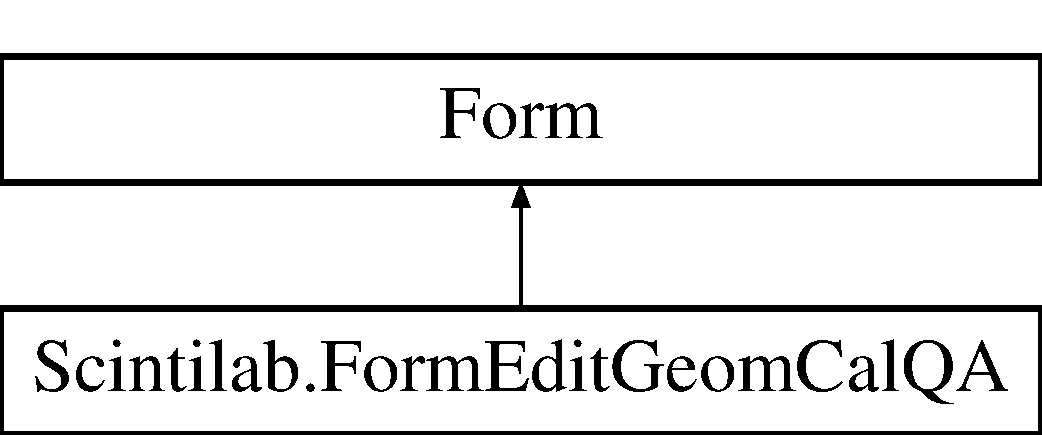
\includegraphics[height=2.000000cm]{class_scintilab_1_1_form_edit_geom_cal_q_a}
\end{center}
\end{figure}
\subsection*{Public medlemsfunksjoner}
\begin{DoxyCompactItemize}
\item 
\hyperlink{class_scintilab_1_1_form_edit_geom_cal_q_a_ab096632a872fc745853f20eab1f40678}{Form\+Edit\+Geom\+Cal\+Q\+A} (string detector, string beaker, ref List$<$ \hyperlink{class_scintilab_1_1_q_a_beaker}{Q\+A\+Beaker} $>$ qabeakers, string caldir)
\end{DoxyCompactItemize}
\subsection*{Public attributter}
\begin{DoxyCompactItemize}
\item 
string \hyperlink{class_scintilab_1_1_form_edit_geom_cal_q_a_a629f62216840fddcd8d5bc5a9ff7dfa1}{Current\+Cal\+File} = \char`\"{}\char`\"{}
\item 
string \hyperlink{class_scintilab_1_1_form_edit_geom_cal_q_a_ad8fe4f87eb8b5fc08f6877b766d4a161}{Current\+Q\+A\+Box} = \char`\"{}\char`\"{}
\item 
string \hyperlink{class_scintilab_1_1_form_edit_geom_cal_q_a_a3b4e607ddbcc2469e57cc99ba9455398}{Selected\+Cal\+File} = \char`\"{}\char`\"{}
\item 
string \hyperlink{class_scintilab_1_1_form_edit_geom_cal_q_a_a3525769c84679debd1f5181ed70e9089}{Selected\+Q\+A\+Box} = \char`\"{}\char`\"{}
\end{DoxyCompactItemize}
\subsection*{Private medlemsfunksjoner}
\begin{DoxyCompactItemize}
\item 
void \hyperlink{class_scintilab_1_1_form_edit_geom_cal_q_a_aa137f32dd12572e97282405fc071b5ca}{btn\+Cancel\+\_\+\+Click} (object sender, Event\+Args e)
\item 
void \hyperlink{class_scintilab_1_1_form_edit_geom_cal_q_a_a2eac66e9cc76af16af67f5144e849eba}{btn\+Ok\+\_\+\+Click} (object sender, Event\+Args e)
\item 
void \hyperlink{class_scintilab_1_1_form_edit_geom_cal_q_a_a93cad2b77f9ed31192cae5ec7bba0e1d}{Form\+Create\+Geom\+Cal\+Q\+A\+\_\+\+Load} (object sender, Event\+Args e)
\end{DoxyCompactItemize}
\subsection*{Private attributter}
\begin{DoxyCompactItemize}
\item 
List$<$ \hyperlink{class_scintilab_1_1_q_a_beaker}{Q\+A\+Beaker} $>$ \hyperlink{class_scintilab_1_1_form_edit_geom_cal_q_a_a8465be0742cd30958c2575a537f28ba2}{m\+Q\+A\+Beakers}
\item 
string \hyperlink{class_scintilab_1_1_form_edit_geom_cal_q_a_a3f8a6138f8dc3a87ff3301739f7aad0a}{m\+Cal\+Dir}
\item 
string \hyperlink{class_scintilab_1_1_form_edit_geom_cal_q_a_afadb7ab76847266dd9281e95ac5d3ce4}{m\+Detector}
\end{DoxyCompactItemize}


\subsection{Detaljert beskrivelse}
Klasse for editering av Beger/\+Calibrasjon/\+Q\+A kombinasjon. 

Definisjon på linje 15 i filen Form\+Edit\+Geom\+Cal\+Q\+A.\+cs.



\subsection{Konstruktør-\/ \& destruktør-\/dokumentasjon}
\hypertarget{class_scintilab_1_1_form_edit_geom_cal_q_a_ab096632a872fc745853f20eab1f40678}{\index{Scintilab\+::\+Form\+Edit\+Geom\+Cal\+Q\+A@{Scintilab\+::\+Form\+Edit\+Geom\+Cal\+Q\+A}!Form\+Edit\+Geom\+Cal\+Q\+A@{Form\+Edit\+Geom\+Cal\+Q\+A}}
\index{Form\+Edit\+Geom\+Cal\+Q\+A@{Form\+Edit\+Geom\+Cal\+Q\+A}!Scintilab\+::\+Form\+Edit\+Geom\+Cal\+Q\+A@{Scintilab\+::\+Form\+Edit\+Geom\+Cal\+Q\+A}}
\subsubsection[{Form\+Edit\+Geom\+Cal\+Q\+A}]{\setlength{\rightskip}{0pt plus 5cm}Scintilab.\+Form\+Edit\+Geom\+Cal\+Q\+A.\+Form\+Edit\+Geom\+Cal\+Q\+A (
\begin{DoxyParamCaption}
\item[{string}]{detector, }
\item[{string}]{beaker, }
\item[{ref List$<$ {\bf Q\+A\+Beaker} $>$}]{qabeakers, }
\item[{string}]{caldir}
\end{DoxyParamCaption}
)\hspace{0.3cm}{\ttfamily [inline]}}}\label{class_scintilab_1_1_form_edit_geom_cal_q_a_ab096632a872fc745853f20eab1f40678}
Konstruktør 

Definisjon på linje 29 i filen Form\+Edit\+Geom\+Cal\+Q\+A.\+cs.


\begin{DoxyCode}
30         \{
31             InitializeComponent();
32             \hyperlink{class_scintilab_1_1_form_edit_geom_cal_q_a_a8465be0742cd30958c2575a537f28ba2}{mQABeakers} = qabeakers;
33             \hyperlink{class_scintilab_1_1_form_edit_geom_cal_q_a_a3f8a6138f8dc3a87ff3301739f7aad0a}{mCalDir} = caldir;
34             \hyperlink{class_scintilab_1_1_form_edit_geom_cal_q_a_afadb7ab76847266dd9281e95ac5d3ce4}{mDetector} = detector;
35             tbGeom.Text = beaker;
36         \}
\end{DoxyCode}


\subsection{Medlemsfunksjon-\/dokumentasjon}
\hypertarget{class_scintilab_1_1_form_edit_geom_cal_q_a_aa137f32dd12572e97282405fc071b5ca}{\index{Scintilab\+::\+Form\+Edit\+Geom\+Cal\+Q\+A@{Scintilab\+::\+Form\+Edit\+Geom\+Cal\+Q\+A}!btn\+Cancel\+\_\+\+Click@{btn\+Cancel\+\_\+\+Click}}
\index{btn\+Cancel\+\_\+\+Click@{btn\+Cancel\+\_\+\+Click}!Scintilab\+::\+Form\+Edit\+Geom\+Cal\+Q\+A@{Scintilab\+::\+Form\+Edit\+Geom\+Cal\+Q\+A}}
\subsubsection[{btn\+Cancel\+\_\+\+Click}]{\setlength{\rightskip}{0pt plus 5cm}void Scintilab.\+Form\+Edit\+Geom\+Cal\+Q\+A.\+btn\+Cancel\+\_\+\+Click (
\begin{DoxyParamCaption}
\item[{object}]{sender, }
\item[{Event\+Args}]{e}
\end{DoxyParamCaption}
)\hspace{0.3cm}{\ttfamily [inline]}, {\ttfamily [private]}}}\label{class_scintilab_1_1_form_edit_geom_cal_q_a_aa137f32dd12572e97282405fc071b5ca}
Hendelse for å avbryte dialog 

Definisjon på linje 41 i filen Form\+Edit\+Geom\+Cal\+Q\+A.\+cs.


\begin{DoxyCode}
42         \{
43             DialogResult = System.Windows.Forms.DialogResult.Cancel;
44             Close();
45         \}
\end{DoxyCode}
\hypertarget{class_scintilab_1_1_form_edit_geom_cal_q_a_a2eac66e9cc76af16af67f5144e849eba}{\index{Scintilab\+::\+Form\+Edit\+Geom\+Cal\+Q\+A@{Scintilab\+::\+Form\+Edit\+Geom\+Cal\+Q\+A}!btn\+Ok\+\_\+\+Click@{btn\+Ok\+\_\+\+Click}}
\index{btn\+Ok\+\_\+\+Click@{btn\+Ok\+\_\+\+Click}!Scintilab\+::\+Form\+Edit\+Geom\+Cal\+Q\+A@{Scintilab\+::\+Form\+Edit\+Geom\+Cal\+Q\+A}}
\subsubsection[{btn\+Ok\+\_\+\+Click}]{\setlength{\rightskip}{0pt plus 5cm}void Scintilab.\+Form\+Edit\+Geom\+Cal\+Q\+A.\+btn\+Ok\+\_\+\+Click (
\begin{DoxyParamCaption}
\item[{object}]{sender, }
\item[{Event\+Args}]{e}
\end{DoxyParamCaption}
)\hspace{0.3cm}{\ttfamily [inline]}, {\ttfamily [private]}}}\label{class_scintilab_1_1_form_edit_geom_cal_q_a_a2eac66e9cc76af16af67f5144e849eba}
Hendelse for O\+K knappen 

Definisjon på linje 50 i filen Form\+Edit\+Geom\+Cal\+Q\+A.\+cs.


\begin{DoxyCode}
51         \{
52             \hyperlink{class_scintilab_1_1_form_edit_geom_cal_q_a_a3b4e607ddbcc2469e57cc99ba9455398}{SelectedCalFile} = cboxCalFiles.Text;
53             \hyperlink{class_scintilab_1_1_form_edit_geom_cal_q_a_a3525769c84679debd1f5181ed70e9089}{SelectedQABox} = cboxQABox.Text;
54             DialogResult = System.Windows.Forms.DialogResult.OK;
55             Close();
56         \}
\end{DoxyCode}
\hypertarget{class_scintilab_1_1_form_edit_geom_cal_q_a_a93cad2b77f9ed31192cae5ec7bba0e1d}{\index{Scintilab\+::\+Form\+Edit\+Geom\+Cal\+Q\+A@{Scintilab\+::\+Form\+Edit\+Geom\+Cal\+Q\+A}!Form\+Create\+Geom\+Cal\+Q\+A\+\_\+\+Load@{Form\+Create\+Geom\+Cal\+Q\+A\+\_\+\+Load}}
\index{Form\+Create\+Geom\+Cal\+Q\+A\+\_\+\+Load@{Form\+Create\+Geom\+Cal\+Q\+A\+\_\+\+Load}!Scintilab\+::\+Form\+Edit\+Geom\+Cal\+Q\+A@{Scintilab\+::\+Form\+Edit\+Geom\+Cal\+Q\+A}}
\subsubsection[{Form\+Create\+Geom\+Cal\+Q\+A\+\_\+\+Load}]{\setlength{\rightskip}{0pt plus 5cm}void Scintilab.\+Form\+Edit\+Geom\+Cal\+Q\+A.\+Form\+Create\+Geom\+Cal\+Q\+A\+\_\+\+Load (
\begin{DoxyParamCaption}
\item[{object}]{sender, }
\item[{Event\+Args}]{e}
\end{DoxyParamCaption}
)\hspace{0.3cm}{\ttfamily [inline]}, {\ttfamily [private]}}}\label{class_scintilab_1_1_form_edit_geom_cal_q_a_a93cad2b77f9ed31192cae5ec7bba0e1d}
Hendelse for lasting av vindu 

Definisjon på linje 61 i filen Form\+Edit\+Geom\+Cal\+Q\+A.\+cs.


\begin{DoxyCode}
62         \{
63             cboxQABox.Items.Add(\textcolor{stringliteral}{""});
64             \textcolor{keywordflow}{foreach} (QABeaker b \textcolor{keywordflow}{in} \hyperlink{class_scintilab_1_1_form_edit_geom_cal_q_a_a8465be0742cd30958c2575a537f28ba2}{mQABeakers})
65                 \textcolor{keywordflow}{if} (b.BeakerName.ToUpper() == tbGeom.Text.ToUpper())
66                     cboxQABox.Items.Add(b.Name);
67 
68             \textcolor{keywordtype}{string}[] files = Directory.GetFiles(\hyperlink{class_scintilab_1_1_form_edit_geom_cal_q_a_a3f8a6138f8dc3a87ff3301739f7aad0a}{mCalDir}, \hyperlink{class_scintilab_1_1_form_edit_geom_cal_q_a_afadb7ab76847266dd9281e95ac5d3ce4}{mDetector} + tbGeom.Text + \textcolor{stringliteral}{"*.CAL"})
      ;
69             \textcolor{keywordflow}{foreach} (\textcolor{keywordtype}{string} fn \textcolor{keywordflow}{in} files)
70                 cboxCalFiles.Items.Add(fn);
71 
72             cboxCalFiles.Text = \hyperlink{class_scintilab_1_1_form_edit_geom_cal_q_a_a629f62216840fddcd8d5bc5a9ff7dfa1}{CurrentCalFile};
73             cboxQABox.Text = \hyperlink{class_scintilab_1_1_form_edit_geom_cal_q_a_ad8fe4f87eb8b5fc08f6877b766d4a161}{CurrentQABox};
74         \}
\end{DoxyCode}


\subsection{Medlemsdata-\/dokumentasjon}
\hypertarget{class_scintilab_1_1_form_edit_geom_cal_q_a_a629f62216840fddcd8d5bc5a9ff7dfa1}{\index{Scintilab\+::\+Form\+Edit\+Geom\+Cal\+Q\+A@{Scintilab\+::\+Form\+Edit\+Geom\+Cal\+Q\+A}!Current\+Cal\+File@{Current\+Cal\+File}}
\index{Current\+Cal\+File@{Current\+Cal\+File}!Scintilab\+::\+Form\+Edit\+Geom\+Cal\+Q\+A@{Scintilab\+::\+Form\+Edit\+Geom\+Cal\+Q\+A}}
\subsubsection[{Current\+Cal\+File}]{\setlength{\rightskip}{0pt plus 5cm}string Scintilab.\+Form\+Edit\+Geom\+Cal\+Q\+A.\+Current\+Cal\+File = \char`\"{}\char`\"{}}}\label{class_scintilab_1_1_form_edit_geom_cal_q_a_a629f62216840fddcd8d5bc5a9ff7dfa1}


Definisjon på linje 21 i filen Form\+Edit\+Geom\+Cal\+Q\+A.\+cs.

\hypertarget{class_scintilab_1_1_form_edit_geom_cal_q_a_ad8fe4f87eb8b5fc08f6877b766d4a161}{\index{Scintilab\+::\+Form\+Edit\+Geom\+Cal\+Q\+A@{Scintilab\+::\+Form\+Edit\+Geom\+Cal\+Q\+A}!Current\+Q\+A\+Box@{Current\+Q\+A\+Box}}
\index{Current\+Q\+A\+Box@{Current\+Q\+A\+Box}!Scintilab\+::\+Form\+Edit\+Geom\+Cal\+Q\+A@{Scintilab\+::\+Form\+Edit\+Geom\+Cal\+Q\+A}}
\subsubsection[{Current\+Q\+A\+Box}]{\setlength{\rightskip}{0pt plus 5cm}string Scintilab.\+Form\+Edit\+Geom\+Cal\+Q\+A.\+Current\+Q\+A\+Box = \char`\"{}\char`\"{}}}\label{class_scintilab_1_1_form_edit_geom_cal_q_a_ad8fe4f87eb8b5fc08f6877b766d4a161}


Definisjon på linje 22 i filen Form\+Edit\+Geom\+Cal\+Q\+A.\+cs.

\hypertarget{class_scintilab_1_1_form_edit_geom_cal_q_a_a3f8a6138f8dc3a87ff3301739f7aad0a}{\index{Scintilab\+::\+Form\+Edit\+Geom\+Cal\+Q\+A@{Scintilab\+::\+Form\+Edit\+Geom\+Cal\+Q\+A}!m\+Cal\+Dir@{m\+Cal\+Dir}}
\index{m\+Cal\+Dir@{m\+Cal\+Dir}!Scintilab\+::\+Form\+Edit\+Geom\+Cal\+Q\+A@{Scintilab\+::\+Form\+Edit\+Geom\+Cal\+Q\+A}}
\subsubsection[{m\+Cal\+Dir}]{\setlength{\rightskip}{0pt plus 5cm}string Scintilab.\+Form\+Edit\+Geom\+Cal\+Q\+A.\+m\+Cal\+Dir\hspace{0.3cm}{\ttfamily [private]}}}\label{class_scintilab_1_1_form_edit_geom_cal_q_a_a3f8a6138f8dc3a87ff3301739f7aad0a}


Definisjon på linje 19 i filen Form\+Edit\+Geom\+Cal\+Q\+A.\+cs.

\hypertarget{class_scintilab_1_1_form_edit_geom_cal_q_a_afadb7ab76847266dd9281e95ac5d3ce4}{\index{Scintilab\+::\+Form\+Edit\+Geom\+Cal\+Q\+A@{Scintilab\+::\+Form\+Edit\+Geom\+Cal\+Q\+A}!m\+Detector@{m\+Detector}}
\index{m\+Detector@{m\+Detector}!Scintilab\+::\+Form\+Edit\+Geom\+Cal\+Q\+A@{Scintilab\+::\+Form\+Edit\+Geom\+Cal\+Q\+A}}
\subsubsection[{m\+Detector}]{\setlength{\rightskip}{0pt plus 5cm}string Scintilab.\+Form\+Edit\+Geom\+Cal\+Q\+A.\+m\+Detector\hspace{0.3cm}{\ttfamily [private]}}}\label{class_scintilab_1_1_form_edit_geom_cal_q_a_afadb7ab76847266dd9281e95ac5d3ce4}


Definisjon på linje 19 i filen Form\+Edit\+Geom\+Cal\+Q\+A.\+cs.

\hypertarget{class_scintilab_1_1_form_edit_geom_cal_q_a_a8465be0742cd30958c2575a537f28ba2}{\index{Scintilab\+::\+Form\+Edit\+Geom\+Cal\+Q\+A@{Scintilab\+::\+Form\+Edit\+Geom\+Cal\+Q\+A}!m\+Q\+A\+Beakers@{m\+Q\+A\+Beakers}}
\index{m\+Q\+A\+Beakers@{m\+Q\+A\+Beakers}!Scintilab\+::\+Form\+Edit\+Geom\+Cal\+Q\+A@{Scintilab\+::\+Form\+Edit\+Geom\+Cal\+Q\+A}}
\subsubsection[{m\+Q\+A\+Beakers}]{\setlength{\rightskip}{0pt plus 5cm}List$<${\bf Q\+A\+Beaker}$>$ Scintilab.\+Form\+Edit\+Geom\+Cal\+Q\+A.\+m\+Q\+A\+Beakers\hspace{0.3cm}{\ttfamily [private]}}}\label{class_scintilab_1_1_form_edit_geom_cal_q_a_a8465be0742cd30958c2575a537f28ba2}


Definisjon på linje 18 i filen Form\+Edit\+Geom\+Cal\+Q\+A.\+cs.

\hypertarget{class_scintilab_1_1_form_edit_geom_cal_q_a_a3b4e607ddbcc2469e57cc99ba9455398}{\index{Scintilab\+::\+Form\+Edit\+Geom\+Cal\+Q\+A@{Scintilab\+::\+Form\+Edit\+Geom\+Cal\+Q\+A}!Selected\+Cal\+File@{Selected\+Cal\+File}}
\index{Selected\+Cal\+File@{Selected\+Cal\+File}!Scintilab\+::\+Form\+Edit\+Geom\+Cal\+Q\+A@{Scintilab\+::\+Form\+Edit\+Geom\+Cal\+Q\+A}}
\subsubsection[{Selected\+Cal\+File}]{\setlength{\rightskip}{0pt plus 5cm}string Scintilab.\+Form\+Edit\+Geom\+Cal\+Q\+A.\+Selected\+Cal\+File = \char`\"{}\char`\"{}}}\label{class_scintilab_1_1_form_edit_geom_cal_q_a_a3b4e607ddbcc2469e57cc99ba9455398}


Definisjon på linje 23 i filen Form\+Edit\+Geom\+Cal\+Q\+A.\+cs.

\hypertarget{class_scintilab_1_1_form_edit_geom_cal_q_a_a3525769c84679debd1f5181ed70e9089}{\index{Scintilab\+::\+Form\+Edit\+Geom\+Cal\+Q\+A@{Scintilab\+::\+Form\+Edit\+Geom\+Cal\+Q\+A}!Selected\+Q\+A\+Box@{Selected\+Q\+A\+Box}}
\index{Selected\+Q\+A\+Box@{Selected\+Q\+A\+Box}!Scintilab\+::\+Form\+Edit\+Geom\+Cal\+Q\+A@{Scintilab\+::\+Form\+Edit\+Geom\+Cal\+Q\+A}}
\subsubsection[{Selected\+Q\+A\+Box}]{\setlength{\rightskip}{0pt plus 5cm}string Scintilab.\+Form\+Edit\+Geom\+Cal\+Q\+A.\+Selected\+Q\+A\+Box = \char`\"{}\char`\"{}}}\label{class_scintilab_1_1_form_edit_geom_cal_q_a_a3525769c84679debd1f5181ed70e9089}


Definisjon på linje 24 i filen Form\+Edit\+Geom\+Cal\+Q\+A.\+cs.



Dokumentasjonen for denne klasse ble generert fra følgende fil\+:\begin{DoxyCompactItemize}
\item 
\hyperlink{_form_edit_geom_cal_q_a_8cs}{Form\+Edit\+Geom\+Cal\+Q\+A.\+cs}\end{DoxyCompactItemize}

\hypertarget{class_scintilab_1_1_form_input_name}{\section{Scintilab.\+Form\+Input\+Name Klasse Referanse}
\label{class_scintilab_1_1_form_input_name}\index{Scintilab.\+Form\+Input\+Name@{Scintilab.\+Form\+Input\+Name}}
}


Klasse for innlesing av et generisk navn fra bruker.  


Arvediagram for Scintilab.\+Form\+Input\+Name\+:\begin{figure}[H]
\begin{center}
\leavevmode
\includegraphics[height=2.000000cm]{class_scintilab_1_1_form_input_name}
\end{center}
\end{figure}
\subsection*{Public medlemsfunksjoner}
\begin{DoxyCompactItemize}
\item 
\hyperlink{class_scintilab_1_1_form_input_name_a0dd3a62578332cfeb90a4fa212950a8d}{Form\+Input\+Name} (string caption)
\end{DoxyCompactItemize}
\subsection*{Public attributter}
\begin{DoxyCompactItemize}
\item 
string \hyperlink{class_scintilab_1_1_form_input_name_aab6aee0df21ac4b5ae151806373b450c}{Selected\+Name}
\end{DoxyCompactItemize}
\subsection*{Private medlemsfunksjoner}
\begin{DoxyCompactItemize}
\item 
void \hyperlink{class_scintilab_1_1_form_input_name_a7ba810a02a7b838eee75429c3c4bf7b1}{btn\+Ok\+\_\+\+Click} (object sender, Event\+Args e)
\item 
void \hyperlink{class_scintilab_1_1_form_input_name_ac25144763079c5cb49403059253bdfd4}{tb\+Name\+\_\+\+Key\+Press} (object sender, Key\+Press\+Event\+Args e)
\end{DoxyCompactItemize}


\subsection{Detaljert beskrivelse}
Klasse for innlesing av et generisk navn fra bruker. 

Definisjon på linje 14 i filen Form\+Input\+Name.\+cs.



\subsection{Konstruktør-\/ \& destruktør-\/dokumentasjon}
\hypertarget{class_scintilab_1_1_form_input_name_a0dd3a62578332cfeb90a4fa212950a8d}{\index{Scintilab\+::\+Form\+Input\+Name@{Scintilab\+::\+Form\+Input\+Name}!Form\+Input\+Name@{Form\+Input\+Name}}
\index{Form\+Input\+Name@{Form\+Input\+Name}!Scintilab\+::\+Form\+Input\+Name@{Scintilab\+::\+Form\+Input\+Name}}
\subsubsection[{Form\+Input\+Name}]{\setlength{\rightskip}{0pt plus 5cm}Scintilab.\+Form\+Input\+Name.\+Form\+Input\+Name (
\begin{DoxyParamCaption}
\item[{string}]{caption}
\end{DoxyParamCaption}
)\hspace{0.3cm}{\ttfamily [inline]}}}\label{class_scintilab_1_1_form_input_name_a0dd3a62578332cfeb90a4fa212950a8d}
Konstruktør 

Definisjon på linje 22 i filen Form\+Input\+Name.\+cs.


\begin{DoxyCode}
23         \{
24             InitializeComponent();
25             lblInfo.Text = caption;
26         \}
\end{DoxyCode}


\subsection{Medlemsfunksjon-\/dokumentasjon}
\hypertarget{class_scintilab_1_1_form_input_name_a7ba810a02a7b838eee75429c3c4bf7b1}{\index{Scintilab\+::\+Form\+Input\+Name@{Scintilab\+::\+Form\+Input\+Name}!btn\+Ok\+\_\+\+Click@{btn\+Ok\+\_\+\+Click}}
\index{btn\+Ok\+\_\+\+Click@{btn\+Ok\+\_\+\+Click}!Scintilab\+::\+Form\+Input\+Name@{Scintilab\+::\+Form\+Input\+Name}}
\subsubsection[{btn\+Ok\+\_\+\+Click}]{\setlength{\rightskip}{0pt plus 5cm}void Scintilab.\+Form\+Input\+Name.\+btn\+Ok\+\_\+\+Click (
\begin{DoxyParamCaption}
\item[{object}]{sender, }
\item[{Event\+Args}]{e}
\end{DoxyParamCaption}
)\hspace{0.3cm}{\ttfamily [inline]}, {\ttfamily [private]}}}\label{class_scintilab_1_1_form_input_name_a7ba810a02a7b838eee75429c3c4bf7b1}
Hendelse for O\+K knappen 

Definisjon på linje 31 i filen Form\+Input\+Name.\+cs.


\begin{DoxyCode}
32         \{
33             \textcolor{keywordflow}{if} (String.IsNullOrEmpty(tbName.Text))
34             \{
35                 MessageBox.Show(\textcolor{stringliteral}{"Du må velge et gyldig navn"});
36                 \textcolor{keywordflow}{return};
37             \}
38             DialogResult = System.Windows.Forms.DialogResult.OK;
39             \hyperlink{class_scintilab_1_1_form_input_name_aab6aee0df21ac4b5ae151806373b450c}{SelectedName} = tbName.Text;
40             Close();
41         \}
\end{DoxyCode}
\hypertarget{class_scintilab_1_1_form_input_name_ac25144763079c5cb49403059253bdfd4}{\index{Scintilab\+::\+Form\+Input\+Name@{Scintilab\+::\+Form\+Input\+Name}!tb\+Name\+\_\+\+Key\+Press@{tb\+Name\+\_\+\+Key\+Press}}
\index{tb\+Name\+\_\+\+Key\+Press@{tb\+Name\+\_\+\+Key\+Press}!Scintilab\+::\+Form\+Input\+Name@{Scintilab\+::\+Form\+Input\+Name}}
\subsubsection[{tb\+Name\+\_\+\+Key\+Press}]{\setlength{\rightskip}{0pt plus 5cm}void Scintilab.\+Form\+Input\+Name.\+tb\+Name\+\_\+\+Key\+Press (
\begin{DoxyParamCaption}
\item[{object}]{sender, }
\item[{Key\+Press\+Event\+Args}]{e}
\end{DoxyParamCaption}
)\hspace{0.3cm}{\ttfamily [inline]}, {\ttfamily [private]}}}\label{class_scintilab_1_1_form_input_name_ac25144763079c5cb49403059253bdfd4}
Hendelse for innlesing av tegn 

Definisjon på linje 46 i filen Form\+Input\+Name.\+cs.


\begin{DoxyCode}
47         \{
48             \textcolor{keywordflow}{if} (e.KeyChar == \textcolor{charliteral}{'\(\backslash\)r'}) \textcolor{comment}{// Hvis tegnet er return}
49             \{
50                 e.Handled = \textcolor{keyword}{true}; \textcolor{comment}{// Dropp "default handler" for denne hendelsen}
51                 \hyperlink{class_scintilab_1_1_form_input_name_a7ba810a02a7b838eee75429c3c4bf7b1}{btnOk\_Click}(sender, e); \textcolor{comment}{// Kjør kode for OK knappen}
52             \}
53         \}
\end{DoxyCode}


\subsection{Medlemsdata-\/dokumentasjon}
\hypertarget{class_scintilab_1_1_form_input_name_aab6aee0df21ac4b5ae151806373b450c}{\index{Scintilab\+::\+Form\+Input\+Name@{Scintilab\+::\+Form\+Input\+Name}!Selected\+Name@{Selected\+Name}}
\index{Selected\+Name@{Selected\+Name}!Scintilab\+::\+Form\+Input\+Name@{Scintilab\+::\+Form\+Input\+Name}}
\subsubsection[{Selected\+Name}]{\setlength{\rightskip}{0pt plus 5cm}string Scintilab.\+Form\+Input\+Name.\+Selected\+Name}}\label{class_scintilab_1_1_form_input_name_aab6aee0df21ac4b5ae151806373b450c}
Lager for valgt navn 

Definisjon på linje 17 i filen Form\+Input\+Name.\+cs.



Dokumentasjonen for denne klasse ble generert fra følgende fil\+:\begin{DoxyCompactItemize}
\item 
\hyperlink{_form_input_name_8cs}{Form\+Input\+Name.\+cs}\end{DoxyCompactItemize}

\hypertarget{class_scintilab_1_1_form_job_report}{\section{Scintilab.\+Form\+Job\+Report Klasse Referanse}
\label{class_scintilab_1_1_form_job_report}\index{Scintilab.\+Form\+Job\+Report@{Scintilab.\+Form\+Job\+Report}}
}


Klasse for visning av jobb rapport.  


Arvediagram for Scintilab.\+Form\+Job\+Report\+:\begin{figure}[H]
\begin{center}
\leavevmode
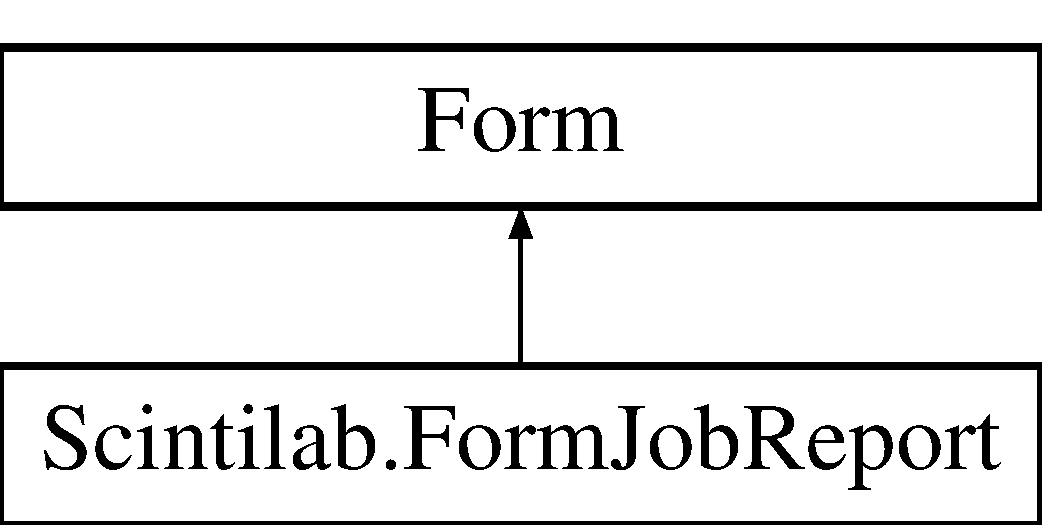
\includegraphics[height=2.000000cm]{class_scintilab_1_1_form_job_report}
\end{center}
\end{figure}
\subsection*{Public medlemsfunksjoner}
\begin{DoxyCompactItemize}
\item 
\hyperlink{class_scintilab_1_1_form_job_report_a2c7a3cd347504010eeb239fc2be05b11}{Form\+Job\+Report} (string base\+Name, string archive\+Name, bool is\+Reanal, ref \hyperlink{class_scintilab_1_1_detector}{Detector} detector, \hyperlink{class_scintilab_1_1_system_parameters}{System\+Parameters} sys\+Par)
\end{DoxyCompactItemize}
\subsection*{Public attributter}
\begin{DoxyCompactItemize}
\item 
bool \hyperlink{class_scintilab_1_1_form_job_report_a03fca1552c0a65c4e526318e880941ff}{Update\+Detectors}
\end{DoxyCompactItemize}
\subsection*{Private medlemsfunksjoner}
\begin{DoxyCompactItemize}
\item 
void \hyperlink{class_scintilab_1_1_form_job_report_a786144f69092cec36454726fdae09776}{Form\+Job\+Report\+\_\+\+Load} (object sender, Event\+Args e)
\item 
void \hyperlink{class_scintilab_1_1_form_job_report_a964b60494d05610029c4844d4712e0e6}{btn\+Delete\+\_\+\+Click} (object sender, Event\+Args e)
\item 
void \hyperlink{class_scintilab_1_1_form_job_report_a2b84afe1ef77debb1f31e8e8e129ebd6}{btn\+Store\+\_\+\+Click} (object sender, Event\+Args e)
\end{DoxyCompactItemize}
\subsection*{Private attributter}
\begin{DoxyCompactItemize}
\item 
string \hyperlink{class_scintilab_1_1_form_job_report_ae2edaad73f9347d9cbc70299ea55c8e4}{Base\+Name}
\item 
string \hyperlink{class_scintilab_1_1_form_job_report_a6befd8e22fc03d7db559bc5819b9001a}{Archive\+Name}
\item 
bool \hyperlink{class_scintilab_1_1_form_job_report_ad6eadf59048ecf2909b4e6c0fd48751f}{Is\+Reanal}
\item 
bool \hyperlink{class_scintilab_1_1_form_job_report_aa9d718d9966b2d6263142d811c4690ef}{has\+Error}
\item 
\hyperlink{class_scintilab_1_1_detector}{Detector} \hyperlink{class_scintilab_1_1_form_job_report_acfd377f5214f1677dbfcee75e848fd3e}{Detector}
\item 
\hyperlink{class_scintilab_1_1_system_parameters}{System\+Parameters} \hyperlink{class_scintilab_1_1_form_job_report_a9d69b66d54f46318d0cd060dd22ef920}{Sys\+Par}
\item 
\hyperlink{class_scintilab_1_1_job_params}{Job\+Params} \hyperlink{class_scintilab_1_1_form_job_report_abf5ab85e5b06729f1494a9e1c6877d7e}{jp} = null
\end{DoxyCompactItemize}


\subsection{Detaljert beskrivelse}
Klasse for visning av jobb rapport. 

Definisjon på linje 16 i filen Form\+Job\+Report.\+cs.



\subsection{Konstruktør-\/ \& destruktør-\/dokumentasjon}
\hypertarget{class_scintilab_1_1_form_job_report_a2c7a3cd347504010eeb239fc2be05b11}{\index{Scintilab\+::\+Form\+Job\+Report@{Scintilab\+::\+Form\+Job\+Report}!Form\+Job\+Report@{Form\+Job\+Report}}
\index{Form\+Job\+Report@{Form\+Job\+Report}!Scintilab\+::\+Form\+Job\+Report@{Scintilab\+::\+Form\+Job\+Report}}
\subsubsection[{Form\+Job\+Report}]{\setlength{\rightskip}{0pt plus 5cm}Scintilab.\+Form\+Job\+Report.\+Form\+Job\+Report (
\begin{DoxyParamCaption}
\item[{string}]{base\+Name, }
\item[{string}]{archive\+Name, }
\item[{bool}]{is\+Reanal, }
\item[{ref {\bf Detector}}]{detector, }
\item[{{\bf System\+Parameters}}]{sys\+Par}
\end{DoxyParamCaption}
)\hspace{0.3cm}{\ttfamily [inline]}}}\label{class_scintilab_1_1_form_job_report_a2c7a3cd347504010eeb239fc2be05b11}
Konstruktør 

Definisjon på linje 29 i filen Form\+Job\+Report.\+cs.


\begin{DoxyCode}
30         \{
31             InitializeComponent();
32             \hyperlink{class_scintilab_1_1_form_job_report_ae2edaad73f9347d9cbc70299ea55c8e4}{BaseName} = baseName;
33             \hyperlink{class_scintilab_1_1_form_job_report_a6befd8e22fc03d7db559bc5819b9001a}{ArchiveName} = archiveName;
34             \hyperlink{class_scintilab_1_1_form_job_report_acfd377f5214f1677dbfcee75e848fd3e}{Detector} = detector;
35             \hyperlink{class_scintilab_1_1_form_job_report_a9d69b66d54f46318d0cd060dd22ef920}{SysPar} = sysPar;
36             \hyperlink{class_scintilab_1_1_form_job_report_ad6eadf59048ecf2909b4e6c0fd48751f}{IsReanal} = isReanal;
37             \hyperlink{class_scintilab_1_1_form_job_report_a03fca1552c0a65c4e526318e880941ff}{UpdateDetectors} = \textcolor{keyword}{false};
38         \}
\end{DoxyCode}


\subsection{Medlemsfunksjon-\/dokumentasjon}
\hypertarget{class_scintilab_1_1_form_job_report_a964b60494d05610029c4844d4712e0e6}{\index{Scintilab\+::\+Form\+Job\+Report@{Scintilab\+::\+Form\+Job\+Report}!btn\+Delete\+\_\+\+Click@{btn\+Delete\+\_\+\+Click}}
\index{btn\+Delete\+\_\+\+Click@{btn\+Delete\+\_\+\+Click}!Scintilab\+::\+Form\+Job\+Report@{Scintilab\+::\+Form\+Job\+Report}}
\subsubsection[{btn\+Delete\+\_\+\+Click}]{\setlength{\rightskip}{0pt plus 5cm}void Scintilab.\+Form\+Job\+Report.\+btn\+Delete\+\_\+\+Click (
\begin{DoxyParamCaption}
\item[{object}]{sender, }
\item[{Event\+Args}]{e}
\end{DoxyParamCaption}
)\hspace{0.3cm}{\ttfamily [inline]}, {\ttfamily [private]}}}\label{class_scintilab_1_1_form_job_report_a964b60494d05610029c4844d4712e0e6}
Hendelse for sletting av jobb 

Definisjon på linje 87 i filen Form\+Job\+Report.\+cs.


\begin{DoxyCode}
88         \{
89             \textcolor{keywordflow}{if} (MessageBox.Show(\textcolor{stringliteral}{"Vil du slette denne jobben?"}, \textcolor{stringliteral}{"Konfirmasjon"}) != 
      System.Windows.Forms.DialogResult.OK)
90                 \textcolor{keywordflow}{return};
91 
92             \textcolor{keywordflow}{if} (File.Exists(\hyperlink{class_scintilab_1_1_form_job_report_ae2edaad73f9347d9cbc70299ea55c8e4}{BaseName} + \textcolor{stringliteral}{".BAT"}))
93                 File.Delete(\hyperlink{class_scintilab_1_1_form_job_report_ae2edaad73f9347d9cbc70299ea55c8e4}{BaseName} + \textcolor{stringliteral}{".BAT"});
94             \textcolor{keywordflow}{if} (File.Exists(\hyperlink{class_scintilab_1_1_form_job_report_ae2edaad73f9347d9cbc70299ea55c8e4}{BaseName} + \textcolor{stringliteral}{".RPT"}))
95                 File.Delete(\hyperlink{class_scintilab_1_1_form_job_report_ae2edaad73f9347d9cbc70299ea55c8e4}{BaseName} + \textcolor{stringliteral}{".RPT"});
96             \textcolor{keywordflow}{if} (File.Exists(\hyperlink{class_scintilab_1_1_form_job_report_ae2edaad73f9347d9cbc70299ea55c8e4}{BaseName} + \textcolor{stringliteral}{".CNF"}))
97                 File.Delete(\hyperlink{class_scintilab_1_1_form_job_report_ae2edaad73f9347d9cbc70299ea55c8e4}{BaseName} + \textcolor{stringliteral}{".CNF"});
98             \textcolor{keywordflow}{if} (File.Exists(\hyperlink{class_scintilab_1_1_form_job_report_ae2edaad73f9347d9cbc70299ea55c8e4}{BaseName} + \textcolor{stringliteral}{".PAR"}))
99                 File.Delete(\hyperlink{class_scintilab_1_1_form_job_report_ae2edaad73f9347d9cbc70299ea55c8e4}{BaseName} + \textcolor{stringliteral}{".PAR"});
100             \textcolor{keywordflow}{if} (File.Exists(\hyperlink{class_scintilab_1_1_form_job_report_ae2edaad73f9347d9cbc70299ea55c8e4}{BaseName} + \textcolor{stringliteral}{".OUT"}))
101                 File.Delete(\hyperlink{class_scintilab_1_1_form_job_report_ae2edaad73f9347d9cbc70299ea55c8e4}{BaseName} + \textcolor{stringliteral}{".OUT"});
102 
103             Close();
104         \}
\end{DoxyCode}
\hypertarget{class_scintilab_1_1_form_job_report_a2b84afe1ef77debb1f31e8e8e129ebd6}{\index{Scintilab\+::\+Form\+Job\+Report@{Scintilab\+::\+Form\+Job\+Report}!btn\+Store\+\_\+\+Click@{btn\+Store\+\_\+\+Click}}
\index{btn\+Store\+\_\+\+Click@{btn\+Store\+\_\+\+Click}!Scintilab\+::\+Form\+Job\+Report@{Scintilab\+::\+Form\+Job\+Report}}
\subsubsection[{btn\+Store\+\_\+\+Click}]{\setlength{\rightskip}{0pt plus 5cm}void Scintilab.\+Form\+Job\+Report.\+btn\+Store\+\_\+\+Click (
\begin{DoxyParamCaption}
\item[{object}]{sender, }
\item[{Event\+Args}]{e}
\end{DoxyParamCaption}
)\hspace{0.3cm}{\ttfamily [inline]}, {\ttfamily [private]}}}\label{class_scintilab_1_1_form_job_report_a2b84afe1ef77debb1f31e8e8e129ebd6}
Hendelse for arkivering av jobb 

Definisjon på linje 109 i filen Form\+Job\+Report.\+cs.


\begin{DoxyCode}
110         \{
111             \textcolor{keywordflow}{if} (\hyperlink{class_scintilab_1_1_form_job_report_aa9d718d9966b2d6263142d811c4690ef}{hasError})
112             \{
113                 DialogResult dialogresult = MessageBox.Show(\textcolor{stringliteral}{"NB! Denne analysen ble fullført med
       feilmelding fra Genie-2000!"} + Environment.NewLine + \textcolor{stringliteral}{"Vil du lagre allikevel?"}, \textcolor{stringliteral}{"Advarsel"}, MessageBoxButtons.YesNo, 
      MessageBoxIcon.Warning);
114                 \textcolor{keywordflow}{if} (dialogresult != DialogResult.Yes)
115                     \textcolor{keywordflow}{return};
116             \}
117 
118             \textcolor{keywordtype}{string} rptFile = \hyperlink{class_scintilab_1_1_form_job_report_ae2edaad73f9347d9cbc70299ea55c8e4}{BaseName} + \textcolor{stringliteral}{".RPT"};
119             \textcolor{keywordtype}{string} cnfFile = \hyperlink{class_scintilab_1_1_form_job_report_ae2edaad73f9347d9cbc70299ea55c8e4}{BaseName} + \textcolor{stringliteral}{".CNF"};
120             \textcolor{keywordtype}{string} parFile = \hyperlink{class_scintilab_1_1_form_job_report_ae2edaad73f9347d9cbc70299ea55c8e4}{BaseName} + \textcolor{stringliteral}{".PAR"};
121             \textcolor{keywordtype}{string} outFile = \hyperlink{class_scintilab_1_1_form_job_report_ae2edaad73f9347d9cbc70299ea55c8e4}{BaseName} + \textcolor{stringliteral}{".OUT"};
122             \textcolor{keywordtype}{string} batFile = \hyperlink{class_scintilab_1_1_form_job_report_ae2edaad73f9347d9cbc70299ea55c8e4}{BaseName} + \textcolor{stringliteral}{".BAT"};
123 
124             \textcolor{keywordflow}{if} (File.Exists(rptFile) && File.Exists(cnfFile) && File.Exists(parFile))
125             \{
126                 \textcolor{keywordflow}{if} (\hyperlink{class_scintilab_1_1_form_job_report_ad6eadf59048ecf2909b4e6c0fd48751f}{IsReanal})
127                 \{
128                     \textcolor{keywordtype}{string} year = \textcolor{stringliteral}{"20"} + jp.SpecRef.Substring(2, 2);
129 
130                     \textcolor{keywordtype}{string} newRpt = Config.ArchiveDir + jp.DetectorName + Path.DirectorySeparatorChar + 
      year + Path.DirectorySeparatorChar + jp.SpecRef + \textcolor{stringliteral}{"-"} + jp.SampleID + \textcolor{stringliteral}{"-"} + jp.Operation + \textcolor{stringliteral}{"-"} + 
      jp.CollectorName + \textcolor{stringliteral}{".RPT"};
131                     \textcolor{keywordtype}{string} newPar = Config.ArchiveDir + jp.DetectorName + Path.DirectorySeparatorChar + 
      year + Path.DirectorySeparatorChar + jp.SpecRef + \textcolor{stringliteral}{"-"} + jp.SampleID + \textcolor{stringliteral}{"-"} + jp.Operation + \textcolor{stringliteral}{"-"} + 
      jp.CollectorName + \textcolor{stringliteral}{".PAR"};
132                     \textcolor{keywordtype}{string} newCnf = Config.ArchiveDir + jp.DetectorName + Path.DirectorySeparatorChar + 
      year + Path.DirectorySeparatorChar + jp.SpecRef + \textcolor{stringliteral}{"-"} + jp.SampleID + \textcolor{stringliteral}{"-"} + jp.Operation + \textcolor{stringliteral}{"-"} + 
      jp.CollectorName + \textcolor{stringliteral}{".CNF"};
133 
134                     \textcolor{keywordtype}{string} oldRpt = \hyperlink{class_scintilab_1_1_form_job_report_a6befd8e22fc03d7db559bc5819b9001a}{ArchiveName} + \textcolor{stringliteral}{".RPT"};
135                     \textcolor{keywordtype}{string} oldPar = \hyperlink{class_scintilab_1_1_form_job_report_a6befd8e22fc03d7db559bc5819b9001a}{ArchiveName} + \textcolor{stringliteral}{".PAR"};
136                     \textcolor{keywordtype}{string} oldCnf = \hyperlink{class_scintilab_1_1_form_job_report_a6befd8e22fc03d7db559bc5819b9001a}{ArchiveName} + \textcolor{stringliteral}{".CNF"};
137 
138                     File.Copy(rptFile, newRpt, \textcolor{keyword}{true});
139                     File.Copy(cnfFile, newCnf, \textcolor{keyword}{true});
140                     File.Copy(parFile, newPar, \textcolor{keyword}{true});
141 
142                     \textcolor{keywordflow}{if} (newRpt != oldRpt)
143                         File.Delete(oldRpt);
144                     \textcolor{keywordflow}{if} (newPar != oldPar)
145                         File.Delete(oldPar);
146                     \textcolor{keywordflow}{if} (newCnf != oldCnf)
147                         File.Delete(oldCnf);
148 
149                     \textcolor{keywordflow}{if} (cbExportLIMS.Checked)
150                         File.Copy(rptFile, SysPar.LimsImport + jp.SampleID + \textcolor{stringliteral}{".NAI.RES"}, \textcolor{keyword}{true});
151 
152                     File.Delete(batFile);
153                     File.Delete(outFile);
154                     lblStatus.Text = \textcolor{stringliteral}{"Reanalyse av spekter "} + jp.SpecRef + \textcolor{stringliteral}{" ble lagret"};
155 
156                     \textcolor{keywordflow}{if} (cbPrint.Checked)
157                     \{
158                         PrintDialog pd = \textcolor{keyword}{new} PrintDialog();
159                         pd.PrinterSettings = \textcolor{keyword}{new} PrinterSettings();
160                         \hyperlink{class_multipad_print_document}{MultipadPrintDocument} printDoc = \textcolor{keyword}{new} 
      \hyperlink{class_multipad_print_document}{MultipadPrintDocument}();
161                         printDoc.PrinterSettings = pd.PrinterSettings;
162                         printDoc.Font = \textcolor{keyword}{new} Font(\textcolor{stringliteral}{"Courier New"}, 9, FontStyle.Regular);
163                         printDoc.Text = File.ReadAllText(rptFile);
164                         printDoc.Print();
165 
166                         \textcolor{comment}{//string cout1;}
167                         \textcolor{comment}{//Utils.RunCommand("REPORT", cnfFile + " /PRINT", out cout1, true);}
168 
169                         \textcolor{keywordtype}{string} cout;
170                         Utils.RunCommand(\textcolor{stringliteral}{"DATAPLOT"}, cnfFile + \textcolor{stringliteral}{" /SCALE="} + SysPar.ReportScaleY + \textcolor{stringliteral}{"
       /XSCALE="} + SysPar.ReportScaleX + \textcolor{stringliteral}{" /ENHPLOT"}, out cout, \textcolor{keyword}{false});
171                     \}
172 
173                     File.Delete(rptFile);
174                     File.Delete(cnfFile);
175                     File.Delete(parFile);
176                 \}
177                 \textcolor{keywordflow}{else}
178                 \{
179                     \textcolor{keywordtype}{string} year = \textcolor{stringliteral}{"20"} + jp.SpecRef.Substring(2, 2);
180                     \textcolor{keywordtype}{string} archiveDir = Config.ArchiveDir + Detector.Name + Path.DirectorySeparatorChar + 
      year + Path.DirectorySeparatorChar;
181                     \textcolor{keywordtype}{string} baseName = jp.SpecRef + \textcolor{stringliteral}{"-"} + jp.SampleID + \textcolor{stringliteral}{"-"} + jp.Operation + \textcolor{stringliteral}{"-"} + 
      jp.CollectorName;
182                     \textcolor{keywordtype}{string} cnfFileDest = archiveDir + baseName + \textcolor{stringliteral}{".CNF"};
183                     \textcolor{keywordtype}{string} rptFileDest = archiveDir + baseName + \textcolor{stringliteral}{".RPT"};
184 
185                     \textcolor{keywordflow}{if} (!Directory.Exists(Config.ArchiveDir + \hyperlink{class_scintilab_1_1_form_job_report_acfd377f5214f1677dbfcee75e848fd3e}{Detector}.
      \hyperlink{class_scintilab_1_1_detector_aeddbda805641ca8d8f8aaa30aea2f3e0}{Name}))
186                         Directory.CreateDirectory(Config.ArchiveDir + \hyperlink{class_scintilab_1_1_form_job_report_acfd377f5214f1677dbfcee75e848fd3e}{Detector}.
      \hyperlink{class_scintilab_1_1_detector_aeddbda805641ca8d8f8aaa30aea2f3e0}{Name});
187                     \textcolor{keywordflow}{if} (!Directory.Exists(Config.ArchiveDir + \hyperlink{class_scintilab_1_1_form_job_report_acfd377f5214f1677dbfcee75e848fd3e}{Detector}.
      \hyperlink{class_scintilab_1_1_detector_aeddbda805641ca8d8f8aaa30aea2f3e0}{Name} + Path.DirectorySeparatorChar + year))
188                         Directory.CreateDirectory(Config.ArchiveDir + \hyperlink{class_scintilab_1_1_form_job_report_acfd377f5214f1677dbfcee75e848fd3e}{Detector}.
      \hyperlink{class_scintilab_1_1_detector_aeddbda805641ca8d8f8aaa30aea2f3e0}{Name} + Path.DirectorySeparatorChar + year);
189 
190                     \textcolor{keywordflow}{if} (cbExportLIMS.Checked)    
191                         File.Copy(rptFile, SysPar.LimsImport + jp.SampleID + \textcolor{stringliteral}{".NAI.RES"}, \textcolor{keyword}{true});
192 
193                     File.Move(rptFile, rptFileDest);
194                     File.Move(cnfFile, cnfFileDest);
195                     File.Move(parFile, archiveDir + baseName + \textcolor{stringliteral}{".PAR"});
196                     
197                     File.Delete(batFile);
198                     File.Delete(outFile);
199                     Detector.SpectrumCounter++;
200                     \hyperlink{class_scintilab_1_1_form_job_report_a03fca1552c0a65c4e526318e880941ff}{UpdateDetectors} = \textcolor{keyword}{true};
201                     lblStatus.Text = \textcolor{stringliteral}{"Jobb for detektor "} + Detector.Name + \textcolor{stringliteral}{" ble arkivert som "} + baseName
      ;
202 
203                     \textcolor{keywordflow}{if} (cbPrint.Checked)
204                     \{
205                         PrintDialog pd = \textcolor{keyword}{new} PrintDialog();
206                         pd.PrinterSettings = \textcolor{keyword}{new} PrinterSettings();
207                         \hyperlink{class_multipad_print_document}{MultipadPrintDocument} printDoc = \textcolor{keyword}{new} 
      \hyperlink{class_multipad_print_document}{MultipadPrintDocument}();
208 
209                         printDoc.PrinterSettings = pd.PrinterSettings;
210                         printDoc.Font = \textcolor{keyword}{new} Font(\textcolor{stringliteral}{"Courier New"}, 9, FontStyle.Regular);
211                         \textcolor{comment}{//printDoc.Text = File.ReadAllText(rptFileDest, Encoding.GetEncoding(865));}
212                         printDoc.Text = File.ReadAllText(rptFileDest, Encoding.GetEncoding(1252));
213                         printDoc.Print();
214 
215                         \textcolor{keywordtype}{string} cout;
216                         Utils.RunCommand(\textcolor{stringliteral}{"DATAPLOT"}, cnfFileDest + \textcolor{stringliteral}{" /SCALE="} + SysPar.ReportScaleY + \textcolor{stringliteral}{"
       /XSCALE="} + SysPar.ReportScaleX + \textcolor{stringliteral}{" /ENHPLOT"}, out cout, \textcolor{keyword}{false});
217                     \}
218                 \}
219             \}
220             \textcolor{keywordflow}{else}
221             \{
222                 MessageBox.Show(\textcolor{stringliteral}{"En eller flere filer ble ikke funnet"});
223             \}
224 
225             Close();
226         \}
\end{DoxyCode}
\hypertarget{class_scintilab_1_1_form_job_report_a786144f69092cec36454726fdae09776}{\index{Scintilab\+::\+Form\+Job\+Report@{Scintilab\+::\+Form\+Job\+Report}!Form\+Job\+Report\+\_\+\+Load@{Form\+Job\+Report\+\_\+\+Load}}
\index{Form\+Job\+Report\+\_\+\+Load@{Form\+Job\+Report\+\_\+\+Load}!Scintilab\+::\+Form\+Job\+Report@{Scintilab\+::\+Form\+Job\+Report}}
\subsubsection[{Form\+Job\+Report\+\_\+\+Load}]{\setlength{\rightskip}{0pt plus 5cm}void Scintilab.\+Form\+Job\+Report.\+Form\+Job\+Report\+\_\+\+Load (
\begin{DoxyParamCaption}
\item[{object}]{sender, }
\item[{Event\+Args}]{e}
\end{DoxyParamCaption}
)\hspace{0.3cm}{\ttfamily [inline]}, {\ttfamily [private]}}}\label{class_scintilab_1_1_form_job_report_a786144f69092cec36454726fdae09776}
Hendelse for lasting av dialog 

Definisjon på linje 43 i filen Form\+Job\+Report.\+cs.


\begin{DoxyCode}
44         \{
45             \textcolor{comment}{// Opprett filbaner}
46             \textcolor{keywordtype}{string} parFile = \hyperlink{class_scintilab_1_1_form_job_report_ae2edaad73f9347d9cbc70299ea55c8e4}{BaseName} + \textcolor{stringliteral}{".PAR"};
47             \textcolor{keywordtype}{string} rptFile = \hyperlink{class_scintilab_1_1_form_job_report_ae2edaad73f9347d9cbc70299ea55c8e4}{BaseName} + \textcolor{stringliteral}{".RPT"};
48             \textcolor{keywordtype}{string} outFile = \hyperlink{class_scintilab_1_1_form_job_report_ae2edaad73f9347d9cbc70299ea55c8e4}{BaseName} + \textcolor{stringliteral}{".OUT"};
49 
50             \textcolor{comment}{// Sjekk at filer finnes}
51             \textcolor{keywordflow}{if} (File.Exists(parFile))
52                 \hyperlink{class_scintilab_1_1_form_job_report_abf5ab85e5b06729f1494a9e1c6877d7e}{jp} = Utils.DeserializeJobParams(parFile);
53 
54             \textcolor{keywordflow}{if}(File.Exists(rptFile))
55                 tbReport.Text= File.ReadAllText(rptFile, Encoding.GetEncoding(1252));
56 
57             \hyperlink{class_scintilab_1_1_form_job_report_aa9d718d9966b2d6263142d811c4690ef}{hasError} = \textcolor{keyword}{false};
58             \textcolor{keywordflow}{if} (File.Exists(outFile))
59             \{
60                 \textcolor{comment}{// Sjekk om standard output filen inneholder ordet "Error"}
61                 tbLog.Text = File.ReadAllText(outFile, Encoding.GetEncoding(1252));
62                 \hyperlink{class_scintilab_1_1_form_job_report_aa9d718d9966b2d6263142d811c4690ef}{hasError} = tbLog.Text.Contains(\textcolor{stringliteral}{"> Error "});
63             \}
64 
65             cbExportLIMS.Checked = \textcolor{keyword}{false};
66             \textcolor{keywordflow}{if} (\hyperlink{class_scintilab_1_1_form_job_report_aa9d718d9966b2d6263142d811c4690ef}{hasError})
67             \{
68                 tabs.SelectedTab = tabError;
69                 cbPrint.Checked = \textcolor{keyword}{false};
70             \}
71             \textcolor{keywordflow}{else}
72             \{
73                 tabs.SelectedTab = tabReport;
74                 cbPrint.Checked = \textcolor{keyword}{true};
75                 \textcolor{keywordflow}{if}(\hyperlink{class_scintilab_1_1_form_job_report_abf5ab85e5b06729f1494a9e1c6877d7e}{jp}.\hyperlink{class_scintilab_1_1_job_params_af7aa58322a6e62ae3cc3bd5d216d389b}{Operation} == \textcolor{stringliteral}{"Sample"})
76                     cbExportLIMS.Checked = \textcolor{keyword}{true};
77             \}
78 
79             \textcolor{comment}{// Fjern selection fra inputfelter}
80             tbReport.Select(0, 0);
81             tbLog.Select(0, 0);
82         \}
\end{DoxyCode}


\subsection{Medlemsdata-\/dokumentasjon}
\hypertarget{class_scintilab_1_1_form_job_report_a6befd8e22fc03d7db559bc5819b9001a}{\index{Scintilab\+::\+Form\+Job\+Report@{Scintilab\+::\+Form\+Job\+Report}!Archive\+Name@{Archive\+Name}}
\index{Archive\+Name@{Archive\+Name}!Scintilab\+::\+Form\+Job\+Report@{Scintilab\+::\+Form\+Job\+Report}}
\subsubsection[{Archive\+Name}]{\setlength{\rightskip}{0pt plus 5cm}string Scintilab.\+Form\+Job\+Report.\+Archive\+Name\hspace{0.3cm}{\ttfamily [private]}}}\label{class_scintilab_1_1_form_job_report_a6befd8e22fc03d7db559bc5819b9001a}


Definisjon på linje 19 i filen Form\+Job\+Report.\+cs.

\hypertarget{class_scintilab_1_1_form_job_report_ae2edaad73f9347d9cbc70299ea55c8e4}{\index{Scintilab\+::\+Form\+Job\+Report@{Scintilab\+::\+Form\+Job\+Report}!Base\+Name@{Base\+Name}}
\index{Base\+Name@{Base\+Name}!Scintilab\+::\+Form\+Job\+Report@{Scintilab\+::\+Form\+Job\+Report}}
\subsubsection[{Base\+Name}]{\setlength{\rightskip}{0pt plus 5cm}string Scintilab.\+Form\+Job\+Report.\+Base\+Name\hspace{0.3cm}{\ttfamily [private]}}}\label{class_scintilab_1_1_form_job_report_ae2edaad73f9347d9cbc70299ea55c8e4}


Definisjon på linje 19 i filen Form\+Job\+Report.\+cs.

\hypertarget{class_scintilab_1_1_form_job_report_acfd377f5214f1677dbfcee75e848fd3e}{\index{Scintilab\+::\+Form\+Job\+Report@{Scintilab\+::\+Form\+Job\+Report}!Detector@{Detector}}
\index{Detector@{Detector}!Scintilab\+::\+Form\+Job\+Report@{Scintilab\+::\+Form\+Job\+Report}}
\subsubsection[{Detector}]{\setlength{\rightskip}{0pt plus 5cm}{\bf Detector} Scintilab.\+Form\+Job\+Report.\+Detector\hspace{0.3cm}{\ttfamily [private]}}}\label{class_scintilab_1_1_form_job_report_acfd377f5214f1677dbfcee75e848fd3e}


Definisjon på linje 21 i filen Form\+Job\+Report.\+cs.

\hypertarget{class_scintilab_1_1_form_job_report_aa9d718d9966b2d6263142d811c4690ef}{\index{Scintilab\+::\+Form\+Job\+Report@{Scintilab\+::\+Form\+Job\+Report}!has\+Error@{has\+Error}}
\index{has\+Error@{has\+Error}!Scintilab\+::\+Form\+Job\+Report@{Scintilab\+::\+Form\+Job\+Report}}
\subsubsection[{has\+Error}]{\setlength{\rightskip}{0pt plus 5cm}bool Scintilab.\+Form\+Job\+Report.\+has\+Error\hspace{0.3cm}{\ttfamily [private]}}}\label{class_scintilab_1_1_form_job_report_aa9d718d9966b2d6263142d811c4690ef}


Definisjon på linje 20 i filen Form\+Job\+Report.\+cs.

\hypertarget{class_scintilab_1_1_form_job_report_ad6eadf59048ecf2909b4e6c0fd48751f}{\index{Scintilab\+::\+Form\+Job\+Report@{Scintilab\+::\+Form\+Job\+Report}!Is\+Reanal@{Is\+Reanal}}
\index{Is\+Reanal@{Is\+Reanal}!Scintilab\+::\+Form\+Job\+Report@{Scintilab\+::\+Form\+Job\+Report}}
\subsubsection[{Is\+Reanal}]{\setlength{\rightskip}{0pt plus 5cm}bool Scintilab.\+Form\+Job\+Report.\+Is\+Reanal\hspace{0.3cm}{\ttfamily [private]}}}\label{class_scintilab_1_1_form_job_report_ad6eadf59048ecf2909b4e6c0fd48751f}


Definisjon på linje 20 i filen Form\+Job\+Report.\+cs.

\hypertarget{class_scintilab_1_1_form_job_report_abf5ab85e5b06729f1494a9e1c6877d7e}{\index{Scintilab\+::\+Form\+Job\+Report@{Scintilab\+::\+Form\+Job\+Report}!jp@{jp}}
\index{jp@{jp}!Scintilab\+::\+Form\+Job\+Report@{Scintilab\+::\+Form\+Job\+Report}}
\subsubsection[{jp}]{\setlength{\rightskip}{0pt plus 5cm}{\bf Job\+Params} Scintilab.\+Form\+Job\+Report.\+jp = null\hspace{0.3cm}{\ttfamily [private]}}}\label{class_scintilab_1_1_form_job_report_abf5ab85e5b06729f1494a9e1c6877d7e}


Definisjon på linje 24 i filen Form\+Job\+Report.\+cs.

\hypertarget{class_scintilab_1_1_form_job_report_a9d69b66d54f46318d0cd060dd22ef920}{\index{Scintilab\+::\+Form\+Job\+Report@{Scintilab\+::\+Form\+Job\+Report}!Sys\+Par@{Sys\+Par}}
\index{Sys\+Par@{Sys\+Par}!Scintilab\+::\+Form\+Job\+Report@{Scintilab\+::\+Form\+Job\+Report}}
\subsubsection[{Sys\+Par}]{\setlength{\rightskip}{0pt plus 5cm}{\bf System\+Parameters} Scintilab.\+Form\+Job\+Report.\+Sys\+Par\hspace{0.3cm}{\ttfamily [private]}}}\label{class_scintilab_1_1_form_job_report_a9d69b66d54f46318d0cd060dd22ef920}


Definisjon på linje 23 i filen Form\+Job\+Report.\+cs.

\hypertarget{class_scintilab_1_1_form_job_report_a03fca1552c0a65c4e526318e880941ff}{\index{Scintilab\+::\+Form\+Job\+Report@{Scintilab\+::\+Form\+Job\+Report}!Update\+Detectors@{Update\+Detectors}}
\index{Update\+Detectors@{Update\+Detectors}!Scintilab\+::\+Form\+Job\+Report@{Scintilab\+::\+Form\+Job\+Report}}
\subsubsection[{Update\+Detectors}]{\setlength{\rightskip}{0pt plus 5cm}bool Scintilab.\+Form\+Job\+Report.\+Update\+Detectors}}\label{class_scintilab_1_1_form_job_report_a03fca1552c0a65c4e526318e880941ff}


Definisjon på linje 22 i filen Form\+Job\+Report.\+cs.



Dokumentasjonen for denne klasse ble generert fra følgende fil\+:\begin{DoxyCompactItemize}
\item 
\hyperlink{_form_job_report_8cs}{Form\+Job\+Report.\+cs}\end{DoxyCompactItemize}

\hypertarget{class_scintilab_1_1_form_login}{\section{Scintilab.\+Form\+Login Klasse Referanse}
\label{class_scintilab_1_1_form_login}\index{Scintilab.\+Form\+Login@{Scintilab.\+Form\+Login}}
}


Klasse for innlogging.  


Arvediagram for Scintilab.\+Form\+Login\+:\begin{figure}[H]
\begin{center}
\leavevmode
\includegraphics[height=2.000000cm]{class_scintilab_1_1_form_login}
\end{center}
\end{figure}
\subsection*{Public medlemsfunksjoner}
\begin{DoxyCompactItemize}
\item 
\hyperlink{class_scintilab_1_1_form_login_a9824d4f0cf40072fcda58524b16c762d}{Form\+Login} ()
\end{DoxyCompactItemize}
\subsection*{Public attributter}
\begin{DoxyCompactItemize}
\item 
string \hyperlink{class_scintilab_1_1_form_login_aba278938a868ca382a657e0c1572a02b}{Username}
\end{DoxyCompactItemize}
\subsection*{Private medlemsfunksjoner}
\begin{DoxyCompactItemize}
\item 
void \hyperlink{class_scintilab_1_1_form_login_a90193599fc2c8ff5c7faee5851063aeb}{btn\+Cancel\+\_\+\+Click} (object sender, Event\+Args e)
\item 
void \hyperlink{class_scintilab_1_1_form_login_a207ac68d96dbc96d570484f30f1d669d}{btn\+Login\+\_\+\+Click} (object sender, Event\+Args e)
\item 
void \hyperlink{class_scintilab_1_1_form_login_aadaa84be09a645732d7beaf53abd6d89}{Form\+Login\+\_\+\+Load} (object sender, Event\+Args e)
\item 
void \hyperlink{class_scintilab_1_1_form_login_a7d992418cc7243b752c826cb9515188e}{tb\+Username\+\_\+\+Key\+Press} (object sender, Key\+Press\+Event\+Args e)
\item 
void \hyperlink{class_scintilab_1_1_form_login_a8c0c4b5c0c2994f179ff216893154fee}{tb\+Password\+\_\+\+Key\+Press} (object sender, Key\+Press\+Event\+Args e)
\end{DoxyCompactItemize}


\subsection{Detaljert beskrivelse}
Klasse for innlogging. 

Definisjon på linje 15 i filen Form\+Login.\+cs.



\subsection{Konstruktør-\/ \& destruktør-\/dokumentasjon}
\hypertarget{class_scintilab_1_1_form_login_a9824d4f0cf40072fcda58524b16c762d}{\index{Scintilab\+::\+Form\+Login@{Scintilab\+::\+Form\+Login}!Form\+Login@{Form\+Login}}
\index{Form\+Login@{Form\+Login}!Scintilab\+::\+Form\+Login@{Scintilab\+::\+Form\+Login}}
\subsubsection[{Form\+Login}]{\setlength{\rightskip}{0pt plus 5cm}Scintilab.\+Form\+Login.\+Form\+Login (
\begin{DoxyParamCaption}
{}
\end{DoxyParamCaption}
)\hspace{0.3cm}{\ttfamily [inline]}}}\label{class_scintilab_1_1_form_login_a9824d4f0cf40072fcda58524b16c762d}
Konstruktør 

Definisjon på linje 23 i filen Form\+Login.\+cs.


\begin{DoxyCode}
24         \{
25             InitializeComponent();
26         \}
\end{DoxyCode}


\subsection{Medlemsfunksjon-\/dokumentasjon}
\hypertarget{class_scintilab_1_1_form_login_a90193599fc2c8ff5c7faee5851063aeb}{\index{Scintilab\+::\+Form\+Login@{Scintilab\+::\+Form\+Login}!btn\+Cancel\+\_\+\+Click@{btn\+Cancel\+\_\+\+Click}}
\index{btn\+Cancel\+\_\+\+Click@{btn\+Cancel\+\_\+\+Click}!Scintilab\+::\+Form\+Login@{Scintilab\+::\+Form\+Login}}
\subsubsection[{btn\+Cancel\+\_\+\+Click}]{\setlength{\rightskip}{0pt plus 5cm}void Scintilab.\+Form\+Login.\+btn\+Cancel\+\_\+\+Click (
\begin{DoxyParamCaption}
\item[{object}]{sender, }
\item[{Event\+Args}]{e}
\end{DoxyParamCaption}
)\hspace{0.3cm}{\ttfamily [inline]}, {\ttfamily [private]}}}\label{class_scintilab_1_1_form_login_a90193599fc2c8ff5c7faee5851063aeb}
Hendelse for å avbryte login 

Definisjon på linje 31 i filen Form\+Login.\+cs.


\begin{DoxyCode}
32         \{
33             \textcolor{comment}{// Sett dialogens resultat til "Cancel"}
34             DialogResult = System.Windows.Forms.DialogResult.Cancel;
35             \textcolor{comment}{// Avslutt Scintilab}
36             Close();
37         \}
\end{DoxyCode}
\hypertarget{class_scintilab_1_1_form_login_a207ac68d96dbc96d570484f30f1d669d}{\index{Scintilab\+::\+Form\+Login@{Scintilab\+::\+Form\+Login}!btn\+Login\+\_\+\+Click@{btn\+Login\+\_\+\+Click}}
\index{btn\+Login\+\_\+\+Click@{btn\+Login\+\_\+\+Click}!Scintilab\+::\+Form\+Login@{Scintilab\+::\+Form\+Login}}
\subsubsection[{btn\+Login\+\_\+\+Click}]{\setlength{\rightskip}{0pt plus 5cm}void Scintilab.\+Form\+Login.\+btn\+Login\+\_\+\+Click (
\begin{DoxyParamCaption}
\item[{object}]{sender, }
\item[{Event\+Args}]{e}
\end{DoxyParamCaption}
)\hspace{0.3cm}{\ttfamily [inline]}, {\ttfamily [private]}}}\label{class_scintilab_1_1_form_login_a207ac68d96dbc96d570484f30f1d669d}
Hendelse for å logge inn 

Definisjon på linje 42 i filen Form\+Login.\+cs.


\begin{DoxyCode}
43         \{
44             PrincipalContext pc = null;
45             \textcolor{keywordtype}{bool} isValid = \textcolor{keyword}{false};
46             \textcolor{keywordflow}{try}
47             \{
48                 \textcolor{comment}{// Opprett kontekst}
49                 pc = \textcolor{keyword}{new} PrincipalContext(ContextType.Domain, \textcolor{stringliteral}{"NRPA"});
50                 \textcolor{comment}{// Valider brukernavn/passord mot AD}
51                 isValid = pc.ValidateCredentials(tbUsername.Text, tbPassword.Text);
52             \}
53             \textcolor{keywordflow}{catch} (Exception ex)
54             \{
55                 \textcolor{comment}{// Noe gikk galt, rapporter til bruker}
56                 MessageBox.Show(ex.Message);
57                 Close(); \textcolor{comment}{// Avslutt Scintilab}
58             \}
59 
60             \textcolor{keywordflow}{if}(!isValid)
61             \{
62                 \textcolor{comment}{// Brukernavn/Passord var ugyldige}
63                 tbUsername.Text = \textcolor{stringliteral}{""};
64                 tbPassword.Text = \textcolor{stringliteral}{""};
65                 lblInfo.Text = \textcolor{stringliteral}{"Ugyldig innlogging"};
66             \}
67             \textcolor{keywordflow}{else}
68             \{
69                 \textcolor{comment}{// Brukernavn/Passord var gyldige}
70                 \hyperlink{class_scintilab_1_1_form_login_aba278938a868ca382a657e0c1572a02b}{Username} = tbUsername.Text;
71                 DialogResult = DialogResult.OK; \textcolor{comment}{// Sett dialogens resultat}
72                 Close(); \textcolor{comment}{// Lukk vindu}
73             \}
74         \}
\end{DoxyCode}
\hypertarget{class_scintilab_1_1_form_login_aadaa84be09a645732d7beaf53abd6d89}{\index{Scintilab\+::\+Form\+Login@{Scintilab\+::\+Form\+Login}!Form\+Login\+\_\+\+Load@{Form\+Login\+\_\+\+Load}}
\index{Form\+Login\+\_\+\+Load@{Form\+Login\+\_\+\+Load}!Scintilab\+::\+Form\+Login@{Scintilab\+::\+Form\+Login}}
\subsubsection[{Form\+Login\+\_\+\+Load}]{\setlength{\rightskip}{0pt plus 5cm}void Scintilab.\+Form\+Login.\+Form\+Login\+\_\+\+Load (
\begin{DoxyParamCaption}
\item[{object}]{sender, }
\item[{Event\+Args}]{e}
\end{DoxyParamCaption}
)\hspace{0.3cm}{\ttfamily [inline]}, {\ttfamily [private]}}}\label{class_scintilab_1_1_form_login_aadaa84be09a645732d7beaf53abd6d89}
Hendelse for lasting av dialog 

Definisjon på linje 79 i filen Form\+Login.\+cs.


\begin{DoxyCode}
80         \{
81             lblInfo.Text = \textcolor{stringliteral}{""};
82             tbUsername.Select();
83         \}
\end{DoxyCode}
\hypertarget{class_scintilab_1_1_form_login_a8c0c4b5c0c2994f179ff216893154fee}{\index{Scintilab\+::\+Form\+Login@{Scintilab\+::\+Form\+Login}!tb\+Password\+\_\+\+Key\+Press@{tb\+Password\+\_\+\+Key\+Press}}
\index{tb\+Password\+\_\+\+Key\+Press@{tb\+Password\+\_\+\+Key\+Press}!Scintilab\+::\+Form\+Login@{Scintilab\+::\+Form\+Login}}
\subsubsection[{tb\+Password\+\_\+\+Key\+Press}]{\setlength{\rightskip}{0pt plus 5cm}void Scintilab.\+Form\+Login.\+tb\+Password\+\_\+\+Key\+Press (
\begin{DoxyParamCaption}
\item[{object}]{sender, }
\item[{Key\+Press\+Event\+Args}]{e}
\end{DoxyParamCaption}
)\hspace{0.3cm}{\ttfamily [inline]}, {\ttfamily [private]}}}\label{class_scintilab_1_1_form_login_a8c0c4b5c0c2994f179ff216893154fee}
Hendelse for inntasting av tegn i felt for passord 

Definisjon på linje 100 i filen Form\+Login.\+cs.


\begin{DoxyCode}
101         \{
102             \textcolor{keywordflow}{if} (e.KeyChar == \textcolor{charliteral}{'\(\backslash\)r'}) \textcolor{comment}{// Hvis tast er return}
103             \{
104                 e.Handled = \textcolor{keyword}{true}; \textcolor{comment}{// Dropp "default handler" for denne hendelsen}
105                 \hyperlink{class_scintilab_1_1_form_login_a207ac68d96dbc96d570484f30f1d669d}{btnLogin\_Click}(sender, e); \textcolor{comment}{// Kjør samme kode som for innlogging}
106             \}
107         \}
\end{DoxyCode}
\hypertarget{class_scintilab_1_1_form_login_a7d992418cc7243b752c826cb9515188e}{\index{Scintilab\+::\+Form\+Login@{Scintilab\+::\+Form\+Login}!tb\+Username\+\_\+\+Key\+Press@{tb\+Username\+\_\+\+Key\+Press}}
\index{tb\+Username\+\_\+\+Key\+Press@{tb\+Username\+\_\+\+Key\+Press}!Scintilab\+::\+Form\+Login@{Scintilab\+::\+Form\+Login}}
\subsubsection[{tb\+Username\+\_\+\+Key\+Press}]{\setlength{\rightskip}{0pt plus 5cm}void Scintilab.\+Form\+Login.\+tb\+Username\+\_\+\+Key\+Press (
\begin{DoxyParamCaption}
\item[{object}]{sender, }
\item[{Key\+Press\+Event\+Args}]{e}
\end{DoxyParamCaption}
)\hspace{0.3cm}{\ttfamily [inline]}, {\ttfamily [private]}}}\label{class_scintilab_1_1_form_login_a7d992418cc7243b752c826cb9515188e}
Hendelse for inntasting av tegn i felt for brukernavn 

Definisjon på linje 88 i filen Form\+Login.\+cs.


\begin{DoxyCode}
89         \{
90             \textcolor{keywordflow}{if} (e.KeyChar == \textcolor{charliteral}{'\(\backslash\)r'}) \textcolor{comment}{// Hvis tast er return}
91             \{
92                 e.Handled = \textcolor{keyword}{true}; \textcolor{comment}{// Dropp "default handler" for denne hendelsen}
93                 tbPassword.Select(); \textcolor{comment}{// Sett felt for passord aktivt}
94             \}
95         \}
\end{DoxyCode}


\subsection{Medlemsdata-\/dokumentasjon}
\hypertarget{class_scintilab_1_1_form_login_aba278938a868ca382a657e0c1572a02b}{\index{Scintilab\+::\+Form\+Login@{Scintilab\+::\+Form\+Login}!Username@{Username}}
\index{Username@{Username}!Scintilab\+::\+Form\+Login@{Scintilab\+::\+Form\+Login}}
\subsubsection[{Username}]{\setlength{\rightskip}{0pt plus 5cm}string Scintilab.\+Form\+Login.\+Username}}\label{class_scintilab_1_1_form_login_aba278938a868ca382a657e0c1572a02b}
Lagring av innskrevet brukernavn 

Definisjon på linje 18 i filen Form\+Login.\+cs.



Dokumentasjonen for denne klasse ble generert fra følgende fil\+:\begin{DoxyCompactItemize}
\item 
\hyperlink{_form_login_8cs}{Form\+Login.\+cs}\end{DoxyCompactItemize}

\hypertarget{class_scintilab_1_1_form_main}{\section{Scintilab.\+Form\+Main Klasse Referanse}
\label{class_scintilab_1_1_form_main}\index{Scintilab.\+Form\+Main@{Scintilab.\+Form\+Main}}
}


Hovedklasse for \hyperlink{namespace_scintilab}{Scintilab}.  


Arvediagram for Scintilab.\+Form\+Main\+:\begin{figure}[H]
\begin{center}
\leavevmode
\includegraphics[height=2.000000cm]{class_scintilab_1_1_form_main}
\end{center}
\end{figure}
\subsection*{Public medlemsfunksjoner}
\begin{DoxyCompactItemize}
\item 
\hyperlink{class_scintilab_1_1_form_main_a7f176c8b5bf31282b730dbfd05155642}{Form\+Main} ()
\item 
bool \hyperlink{class_scintilab_1_1_form_main_ac34ad4400cb8a7b5d38feca1f620b3cb}{Generate\+Bat\+From\+Params} (\hyperlink{class_scintilab_1_1_job_params}{Job\+Params} jp)
\item 
void \hyperlink{class_scintilab_1_1_form_main_ab1eef461219a3b724d3bf3af0cd68e94}{Generate\+Reanal\+Bat\+From\+Params} (string temp\+Name, string archive\+Name, \hyperlink{class_scintilab_1_1_job_params}{Job\+Params} jp)
\end{DoxyCompactItemize}
\subsection*{Public attributter}
\begin{DoxyCompactItemize}
\item 
List$<$ \hyperlink{class_scintilab_1_1_detector}{Detector} $>$ \hyperlink{class_scintilab_1_1_form_main_a88f16134102d9e4c5630adf5ff97f090}{Detectors} = null
\end{DoxyCompactItemize}
\subsection*{Private medlemsfunksjoner}
\begin{DoxyCompactItemize}
\item 
\hyperlink{class_scintilab_1_1_detector}{Detector} \hyperlink{class_scintilab_1_1_form_main_aff4482e0919480013a53fe56cfb374ba}{get\+Detector\+By\+Name} (string name)
\item 
\hyperlink{class_scintilab_1_1_beaker}{Beaker} \hyperlink{class_scintilab_1_1_form_main_a28d6ae4e27996e005e989b7256a45460}{get\+Beaker\+By\+Name} (string name)
\item 
\hyperlink{class_scintilab_1_1_q_a_beaker}{Q\+A\+Beaker} \hyperlink{class_scintilab_1_1_form_main_ae8b1f6bb6a734ec6ad54794d345ce650}{get\+Q\+A\+Beaker\+By\+Name} (string name)
\item 
void \hyperlink{class_scintilab_1_1_form_main_a79453298b8521054e8012d9df6fe6b93}{clear\+Adm\+Detectors} ()
\item 
void \hyperlink{class_scintilab_1_1_form_main_af1716116c6d9b7a6900fb3ac10b7cf26}{clear\+Adm\+Beakers} ()
\item 
void \hyperlink{class_scintilab_1_1_form_main_a94e0c785ff92478f3bb21311a6bdf50f}{clear\+Adm\+Q\+A\+Beakers} ()
\item 
void \hyperlink{class_scintilab_1_1_form_main_a01c213a0d1456773b92d4d431a9d1cdb}{clear\+Samp\+Params} ()
\item 
void \hyperlink{class_scintilab_1_1_form_main_ace8f1fb51afa44804deec60a6dc42bcb}{populate\+Samp\+Geom} (string det\+Name)
\item 
void \hyperlink{class_scintilab_1_1_form_main_a2d2ec0fa77e4dd0a81bb186b8021b210}{populate\+Samp\+Geom\+With\+Q\+A} (string det\+Name)
\item 
void \hyperlink{class_scintilab_1_1_form_main_ab744904cac6a4bf90ebbe326b658e2e5}{add\+Cal\+Files\+To\+Samp} (\hyperlink{class_scintilab_1_1_detector}{Detector} d, string beaker\+Name)
\item 
void \hyperlink{class_scintilab_1_1_form_main_a14289005c3867f1744618030dc33d79c}{Menu\+Item\+Exit\+\_\+\+Click} (object sender, Event\+Args e)
\item 
void \hyperlink{class_scintilab_1_1_form_main_a7919f1d4c3819a3c85df4107bbf82a59}{Update\+Detector\+Lists} ()
\item 
void \hyperlink{class_scintilab_1_1_form_main_a6c96beb015193d225dd65035759f8484}{Form\+Main\+\_\+\+Load} (object sender, Event\+Args e)
\item 
void \hyperlink{class_scintilab_1_1_form_main_ab8ea1ca503bf5fecfdf241a6813fbbca}{Application\+\_\+\+Idle} (object sender, System.\+Event\+Args e)
\item 
void \hyperlink{class_scintilab_1_1_form_main_ab53847bf056f4cec151f5ad5d5e0ceec}{On\+Jobs\+Changed} (object source, File\+System\+Event\+Args e)
\item 
bool \hyperlink{class_scintilab_1_1_form_main_a158d3b89f669d3b2a24ba750caef3eec}{Lookup\+New\+Detectors} ()
\item 
bool \hyperlink{class_scintilab_1_1_form_main_a072f08bc198944051dffd3d8fac4cc9d}{check\+For\+Errors} (string filename)
\item 
void \hyperlink{class_scintilab_1_1_form_main_a26420269c1a616c31de7521deebbef5f}{update\+Grid\+Jobs} ()
\item 
void \hyperlink{class_scintilab_1_1_form_main_a9cfeb3e22a98715b97f61b779e56b260}{btn\+Menu\+Jobs\+\_\+\+Click} (object sender, Event\+Args e)
\item 
void \hyperlink{class_scintilab_1_1_form_main_a41ead05b3b898979155de24a559af523}{btn\+Menu\+Archive\+\_\+\+Click} (object sender, Event\+Args e)
\item 
void \hyperlink{class_scintilab_1_1_form_main_a2432aabab8e149c90ce3c5de9779d33a}{Menu\+Item\+Admin\+\_\+\+Click} (object sender, Event\+Args e)
\item 
void \hyperlink{class_scintilab_1_1_form_main_aca32a54e95297f770c9022441cb74a90}{btn\+Back\+\_\+\+Click} (object sender, Event\+Args e)
\item 
void \hyperlink{class_scintilab_1_1_form_main_aa8c918f5dc9b6c05a02109bf41eec156}{tabs\+\_\+\+Selected\+Index\+Changed} (object sender, Event\+Args e)
\item 
bool \hyperlink{class_scintilab_1_1_form_main_a0fc122d41cfd2269400517c27dfb2aa3}{Detector\+Has\+Job} (\hyperlink{class_scintilab_1_1_detector}{Detector} d)
\item 
void \hyperlink{class_scintilab_1_1_form_main_a4793aee20cbfead78e08f36997b9837c}{lv\+Detectors\+\_\+\+Selected\+Index\+Changed} (object sender, Event\+Args e)
\item 
void \hyperlink{class_scintilab_1_1_form_main_ad85e690e8d5fa96cbf9c0a7632bd7140}{Set\+Sample\+Fields\+Status} (bool enable)
\item 
void \hyperlink{class_scintilab_1_1_form_main_a566e7914e95ee64d886ef430796b9f64}{btn\+Samp\+Read\+Barcode\+\_\+\+Click} (object sender, Event\+Args e)
\item 
void \hyperlink{class_scintilab_1_1_form_main_ab155e944ae752fdde630c1f4a4827902}{lb\+Adm\+Det\+List\+\_\+\+Selected\+Index\+Changed} (object sender, Event\+Args e)
\item 
void \hyperlink{class_scintilab_1_1_form_main_ae3ae1f6cec4d61f964b0c4e0a4468a4c}{lb\+Adm\+Geom\+List\+\_\+\+Selected\+Index\+Changed} (object sender, Event\+Args e)
\item 
void \hyperlink{class_scintilab_1_1_form_main_adb8fdd0575ceff94bb6a842e25b9f0f1}{lb\+Adm\+Q\+A\+List\+\_\+\+Selected\+Index\+Changed} (object sender, Event\+Args e)
\item 
void \hyperlink{class_scintilab_1_1_form_main_a262b28336ad08680d43100f4cd5afe03}{cbox\+Samp\+Geom\+\_\+\+Selected\+Index\+Changed} (object sender, Event\+Args e)
\item 
void \hyperlink{class_scintilab_1_1_form_main_a182cf23da0489ee71d0fd1a90abacdf0}{btn\+Adm\+Det\+Save\+\_\+\+Click} (object sender, Event\+Args e)
\item 
string \hyperlink{class_scintilab_1_1_form_main_aaac85ee2e1b1f107ed9f653435c6b025}{get\+File} (string title, string dir, string filter)
\item 
string \hyperlink{class_scintilab_1_1_form_main_af1dbdd5d9d15c9a665a249394091b4f1}{get\+Folder} (string title)
\item 
void \hyperlink{class_scintilab_1_1_form_main_adaf37500d9e85e8a8fa5494e0070994c}{btn\+Adm\+Det\+Bkg\+Sub\+\_\+\+Click} (object sender, Event\+Args e)
\item 
void \hyperlink{class_scintilab_1_1_form_main_a675dfb6e115d582b0158853c9ac698e2}{btn\+Adm\+Det\+N\+I\+D\+Lib\+\_\+\+Click} (object sender, Event\+Args e)
\item 
void \hyperlink{class_scintilab_1_1_form_main_a45d3024dfac28a98d3f282079dd53206}{btn\+Adm\+Det\+Geom\+Cal\+Add\+\_\+\+Click} (object sender, Event\+Args e)
\item 
void \hyperlink{class_scintilab_1_1_form_main_ad3fe00a88fb8da2b88832fc60e7fd674}{btn\+Adm\+Det\+Geom\+Cal\+Edit\+\_\+\+Click} (object sender, Event\+Args e)
\item 
void \hyperlink{class_scintilab_1_1_form_main_a93fd0bccb6ec721eca356f868939e68b}{populate\+Sample\+From\+File} (string filename)
\item 
void \hyperlink{class_scintilab_1_1_form_main_a12209de63c7a7c7d6790466e9be3edd5}{btn\+Samp\+Start\+\_\+\+Click} (object sender, Event\+Args e)
\item 
string \hyperlink{class_scintilab_1_1_form_main_ad8de93638ebc50f712d85af269ba383d}{get\+Q\+A\+Box\+From\+Detector} (\hyperlink{class_scintilab_1_1_detector}{Detector} d, string geom)
\item 
void \hyperlink{class_scintilab_1_1_form_main_a6306e9b64d524deb6b9f5fb0a6259647}{btn\+Job\+Open\+Spectrum\+\_\+\+Click} (object sender, Event\+Args e)
\item 
void \hyperlink{class_scintilab_1_1_form_main_adaef6dd7659666d44b846de21d5b14df}{btn\+Jobs\+Show\+Output\+\_\+\+Click} (object sender, Event\+Args e)
\item 
void \hyperlink{class_scintilab_1_1_form_main_a953db9b2ca7c1a92c327871b4a448934}{btn\+Adm\+Genie\+Folder\+\_\+\+Click} (object sender, Event\+Args e)
\item 
void \hyperlink{class_scintilab_1_1_form_main_ae1b0cb30ebcecd34d4ad1a59cbce6d38}{btn\+Adm\+Save\+\_\+\+Click} (object sender, Event\+Args e)
\item 
void \hyperlink{class_scintilab_1_1_form_main_a6e20ae5c9d1546f174e52e347657e6db}{btn\+Adm\+Template\+\_\+\+Click} (object sender, Event\+Args e)
\item 
void \hyperlink{class_scintilab_1_1_form_main_ab14307d4fa2fc950a86baf6b0a56514c}{btn\+Adm\+L\+I\+M\+S\+Import\+\_\+\+Click} (object sender, Event\+Args e)
\item 
void \hyperlink{class_scintilab_1_1_form_main_ad9f04197f41acec2571a81ca2966069f}{btn\+Adm\+L\+I\+M\+S\+Export\+\_\+\+Click} (object sender, Event\+Args e)
\item 
void \hyperlink{class_scintilab_1_1_form_main_a99614128337091c0589a30ba511397b6}{btn\+Adm\+Det\+Geom\+Cal\+Delete\+\_\+\+Click} (object sender, Event\+Args e)
\item 
void \hyperlink{class_scintilab_1_1_form_main_a947d821789ec1a55af6af94c2faea82d}{tv\+Archive\+\_\+\+After\+Select} (object sender, Tree\+View\+Event\+Args e)
\item 
void \hyperlink{class_scintilab_1_1_form_main_a9e03fe4c4af959f108ded057804996f6}{btn\+Adm\+Q\+A\+New\+\_\+\+Click} (object sender, Event\+Args e)
\item 
void \hyperlink{class_scintilab_1_1_form_main_af337ca12fa73a28ae1c34b7169777d69}{btn\+Archive\+Reanal\+\_\+\+Click} (object sender, Event\+Args e)
\item 
void \hyperlink{class_scintilab_1_1_form_main_a267fcaa644ed5e84053883a9164adf6b}{btn\+Open\+Q\+A\+Plot\+\_\+\+Click} (object sender, Event\+Args e)
\item 
void \hyperlink{class_scintilab_1_1_form_main_a0a801bd487880ec77bdd03a36926a660}{btn\+Job\+Show\+\_\+\+Click} (object sender, Event\+Args e)
\item 
void \hyperlink{class_scintilab_1_1_form_main_a7cef2942c91ce3e6d209aec5e17f8751}{btn\+Samp\+Anal\+Bkg\+Sub\+\_\+\+Click} (object sender, Event\+Args e)
\item 
void \hyperlink{class_scintilab_1_1_form_main_aa1b4a5be131daa0da4742d5011088756}{btn\+Samp\+Anal\+N\+I\+D\+Lib\+\_\+\+Click} (object sender, Event\+Args e)
\item 
void \hyperlink{class_scintilab_1_1_form_main_a5a12d967594f000e71f7f8e79eded8d4}{btn\+Archive\+Show\+Report\+\_\+\+Click} (object sender, Event\+Args e)
\item 
void \hyperlink{class_scintilab_1_1_form_main_a732f051d849b79cd620a0f699d3dcaeb}{btn\+Archive\+Show\+Params\+\_\+\+Click} (object sender, Event\+Args e)
\item 
void \hyperlink{class_scintilab_1_1_form_main_a73fdda90a8617b61e3de31be6b659564}{btn\+Archive\+Print\+\_\+\+Click} (object sender, Event\+Args e)
\item 
void \hyperlink{class_scintilab_1_1_form_main_a6d7ebeb5c9dadf53b29f7faccdad6102}{Menu\+Item\+Logout\+\_\+\+Click} (object sender, Event\+Args e)
\item 
bool \hyperlink{class_scintilab_1_1_form_main_a6cb8b069c0d1b488dbf0abef2b8fcfb3}{check\+Valid\+Integer} (char ch)
\item 
bool \hyperlink{class_scintilab_1_1_form_main_ac7955a16efd0a7b15614c904db1c4d20}{check\+Valid\+Decimal} (string txt, char ch)
\item 
void \hyperlink{class_scintilab_1_1_form_main_ae3cd051584a2767807a47d1d45a13d4e}{Integer\+\_\+\+Key\+Press} (object sender, Key\+Press\+Event\+Args e)
\item 
void \hyperlink{class_scintilab_1_1_form_main_a8b2aed106bf6da84eade77654137b723}{Decimal\+\_\+\+Key\+Press} (object sender, Key\+Press\+Event\+Args e)
\item 
void \hyperlink{class_scintilab_1_1_form_main_a6b4990d68fbc5c9c543e4403f5630229}{btn\+Adm\+Q\+A\+Save\+\_\+\+Click} (object sender, Event\+Args e)
\item 
void \hyperlink{class_scintilab_1_1_form_main_a52f26a9255f72e013f3b2067905838ca}{btn\+Adm\+Geom\+Save\+\_\+\+Click} (object sender, Event\+Args e)
\item 
void \hyperlink{class_scintilab_1_1_form_main_a5aefdcf34c90024ca153c8b8f1200c01}{populate\+Sample\+View} (\hyperlink{class_scintilab_1_1_selection_info}{Selection\+Info} si)
\item 
void \hyperlink{class_scintilab_1_1_form_main_a73ffa9e06d5936a593bf11d78f6abbc0}{btn\+Menu\+Sample\+\_\+\+Click} (object sender, Event\+Args e)
\item 
void \hyperlink{class_scintilab_1_1_form_main_a909462e7826215219d895954dec393c3}{btn\+Archive\+Create\+Bkg\+\_\+\+Click} (object sender, Event\+Args e)
\item 
void \hyperlink{class_scintilab_1_1_form_main_a91cb583dc09f198b098c9d99647053e1}{btn\+Adm\+Geo\+New\+\_\+\+Click} (object sender, Event\+Args e)
\item 
void \hyperlink{class_scintilab_1_1_form_main_a477fe2e53536fb7a63e77656fb196cd4}{btn\+Archive\+Show\+Spectrum\+\_\+\+Click} (object sender, Event\+Args e)
\end{DoxyCompactItemize}
\subsection*{Private attributter}
\begin{DoxyCompactItemize}
\item 
\hyperlink{class_scintilab_1_1_system_parameters}{System\+Parameters} \hyperlink{class_scintilab_1_1_form_main_ad41498eb151a72c77ad94c7285d0f506}{Sys\+Par} = null
\item 
List$<$ \hyperlink{class_scintilab_1_1_beaker}{Beaker} $>$ \hyperlink{class_scintilab_1_1_form_main_aaff2cbfd906f576997bce08ece74dae8}{Beakers} = null
\item 
List$<$ \hyperlink{class_scintilab_1_1_q_a_beaker}{Q\+A\+Beaker} $>$ \hyperlink{class_scintilab_1_1_form_main_af318208d55e4a144a14abde1adc7559d}{Q\+A\+Beakers} = null
\item 
\hyperlink{class_scintilab_1_1_selection_info}{Selection\+Info} \hyperlink{class_scintilab_1_1_form_main_a57c8340ae2caaec775ad70d8036514fb}{Sel\+Info} = new \hyperlink{class_scintilab_1_1_selection_info}{Selection\+Info}()
\item 
File\+System\+Watcher \hyperlink{class_scintilab_1_1_form_main_a0331bda673387e5d96deebd876575d1d}{watcher} = new File\+System\+Watcher()
\item 
bool \hyperlink{class_scintilab_1_1_form_main_a751a47b90ebd11367991fc095818d8a2}{update\+Jobs} = false
\item 
bool \hyperlink{class_scintilab_1_1_form_main_a389e9c6697c567d84058d178053a837c}{is\+Reanal} = false
\end{DoxyCompactItemize}


\subsection{Detaljert beskrivelse}
Hovedklasse for \hyperlink{namespace_scintilab}{Scintilab}. 

Definisjon på linje 19 i filen Form\+Main.\+cs.



\subsection{Konstruktør-\/ \& destruktør-\/dokumentasjon}
\hypertarget{class_scintilab_1_1_form_main_a7f176c8b5bf31282b730dbfd05155642}{\index{Scintilab\+::\+Form\+Main@{Scintilab\+::\+Form\+Main}!Form\+Main@{Form\+Main}}
\index{Form\+Main@{Form\+Main}!Scintilab\+::\+Form\+Main@{Scintilab\+::\+Form\+Main}}
\subsubsection[{Form\+Main}]{\setlength{\rightskip}{0pt plus 5cm}Scintilab.\+Form\+Main.\+Form\+Main (
\begin{DoxyParamCaption}
{}
\end{DoxyParamCaption}
)\hspace{0.3cm}{\ttfamily [inline]}}}\label{class_scintilab_1_1_form_main_a7f176c8b5bf31282b730dbfd05155642}
Konstruktør 

Definisjon på linje 41 i filen Form\+Main.\+cs.


\begin{DoxyCode}
42         \{
43             InitializeComponent();
44         \}
\end{DoxyCode}


\subsection{Medlemsfunksjon-\/dokumentasjon}
\hypertarget{class_scintilab_1_1_form_main_ab744904cac6a4bf90ebbe326b658e2e5}{\index{Scintilab\+::\+Form\+Main@{Scintilab\+::\+Form\+Main}!add\+Cal\+Files\+To\+Samp@{add\+Cal\+Files\+To\+Samp}}
\index{add\+Cal\+Files\+To\+Samp@{add\+Cal\+Files\+To\+Samp}!Scintilab\+::\+Form\+Main@{Scintilab\+::\+Form\+Main}}
\subsubsection[{add\+Cal\+Files\+To\+Samp}]{\setlength{\rightskip}{0pt plus 5cm}void Scintilab.\+Form\+Main.\+add\+Cal\+Files\+To\+Samp (
\begin{DoxyParamCaption}
\item[{{\bf Detector}}]{d, }
\item[{string}]{beaker\+Name}
\end{DoxyParamCaption}
)\hspace{0.3cm}{\ttfamily [inline]}, {\ttfamily [private]}}}\label{class_scintilab_1_1_form_main_ab744904cac6a4bf90ebbe326b658e2e5}
Fyll inn gyldige .C\+A\+L filer for valg detektor og beger


\begin{DoxyParams}{Parametre}
{\em d} & Valgt detektor \\
\hline
{\em beaker\+Name} & Navn på valgt beger \\
\hline
\end{DoxyParams}


Definisjon på linje 286 i filen Form\+Main.\+cs.


\begin{DoxyCode}
287         \{
288             cboxSampAdvCal.Items.Clear(); \textcolor{comment}{// Tøm dropdown for calbreringsfiler}
289             \textcolor{comment}{// Opprett filnavnfilter for kalibreringsfiler}
290             \textcolor{keywordtype}{string} filter = d.Name + beakerName + \textcolor{stringliteral}{"*.CAL"};
291             \textcolor{comment}{// Opprett liste over filbaner til kalibreringsfiler som tilfredstiller filteret}
292             \textcolor{keywordtype}{string}[] files = Directory.GetFiles(\hyperlink{class_scintilab_1_1_config_a8bb782f1eebd5ba14d686c57bc981298}{Config.CalDir}, filter);
293             \textcolor{comment}{// Legg til kalibreringsfilene i dropdown (kun filnavnet)}
294             \textcolor{keywordflow}{foreach} (\textcolor{keywordtype}{string} fn \textcolor{keywordflow}{in} files)
295                 cboxSampAdvCal.Items.Add(Path.GetFileName(fn));
296 
297             \textcolor{comment}{// Sett aktivt beger i dropdown hvis det finnes i detektor definisjonen}
298             \textcolor{keywordflow}{for} (\textcolor{keywordtype}{int} i = 0; i < d.BeakerInfoList.Count; i++)
299                 \textcolor{keywordflow}{if} (d.BeakerInfoList[i].BeakerName == beakerName)
300                     cboxSampAdvCal.Text = Path.GetFileName(d.BeakerInfoList[i].CalibrationFile);
301         \}
\end{DoxyCode}
\hypertarget{class_scintilab_1_1_form_main_ab8ea1ca503bf5fecfdf241a6813fbbca}{\index{Scintilab\+::\+Form\+Main@{Scintilab\+::\+Form\+Main}!Application\+\_\+\+Idle@{Application\+\_\+\+Idle}}
\index{Application\+\_\+\+Idle@{Application\+\_\+\+Idle}!Scintilab\+::\+Form\+Main@{Scintilab\+::\+Form\+Main}}
\subsubsection[{Application\+\_\+\+Idle}]{\setlength{\rightskip}{0pt plus 5cm}void Scintilab.\+Form\+Main.\+Application\+\_\+\+Idle (
\begin{DoxyParamCaption}
\item[{object}]{sender, }
\item[{System.\+Event\+Args}]{e}
\end{DoxyParamCaption}
)\hspace{0.3cm}{\ttfamily [inline]}, {\ttfamily [private]}}}\label{class_scintilab_1_1_form_main_ab8ea1ca503bf5fecfdf241a6813fbbca}
Hendelse for program i inaktiv tilstand 

Definisjon på linje 523 i filen Form\+Main.\+cs.


\begin{DoxyCode}
524         \{
525             \textcolor{comment}{// Sjekk om jobb katalogen trenger oppdatering}
526             \textcolor{keywordflow}{if} (\hyperlink{class_scintilab_1_1_form_main_a751a47b90ebd11367991fc095818d8a2}{updateJobs})
527             \{
528                 \hyperlink{class_scintilab_1_1_form_main_a751a47b90ebd11367991fc095818d8a2}{updateJobs} = \textcolor{keyword}{false};
529                 \hyperlink{class_scintilab_1_1_form_main_a26420269c1a616c31de7521deebbef5f}{updateGridJobs}(); \textcolor{comment}{// Oppdater jobb informasjon}
530             \}
531 
532             \textcolor{comment}{// Diverse oppdateringer for grensesnittet}
533             \textcolor{keywordflow}{if} (tabs.SelectedTab == tabAdmin && tabsAdmin.SelectedTab == tabAdminQA && btnAdmQANew.Visible 
      == \textcolor{keyword}{false})
534                 btnAdmQANew.Visible = \textcolor{keyword}{true};
535             \textcolor{keywordflow}{else} \textcolor{keywordflow}{if}((tabs.SelectedTab != tabAdmin || tabsAdmin.SelectedTab != tabAdminQA) && btnAdmQANew.
      Visible == \textcolor{keyword}{true})
536                 btnAdmQANew.Visible = \textcolor{keyword}{false};
537 
538             \textcolor{keywordflow}{if} (tabs.SelectedTab == tabAdmin && tabsAdmin.SelectedTab == tabAdminGeom && btnAdmGeoNew.
      Visible == \textcolor{keyword}{false})
539                 btnAdmGeoNew.Visible = \textcolor{keyword}{true};
540             \textcolor{keywordflow}{else} \textcolor{keywordflow}{if} ((tabs.SelectedTab != tabAdmin || tabsAdmin.SelectedTab != tabAdminGeom) && 
      btnAdmGeoNew.Visible == \textcolor{keyword}{true})
541                 btnAdmGeoNew.Visible = \textcolor{keyword}{false};
542         \}
\end{DoxyCode}
\hypertarget{class_scintilab_1_1_form_main_adaf37500d9e85e8a8fa5494e0070994c}{\index{Scintilab\+::\+Form\+Main@{Scintilab\+::\+Form\+Main}!btn\+Adm\+Det\+Bkg\+Sub\+\_\+\+Click@{btn\+Adm\+Det\+Bkg\+Sub\+\_\+\+Click}}
\index{btn\+Adm\+Det\+Bkg\+Sub\+\_\+\+Click@{btn\+Adm\+Det\+Bkg\+Sub\+\_\+\+Click}!Scintilab\+::\+Form\+Main@{Scintilab\+::\+Form\+Main}}
\subsubsection[{btn\+Adm\+Det\+Bkg\+Sub\+\_\+\+Click}]{\setlength{\rightskip}{0pt plus 5cm}void Scintilab.\+Form\+Main.\+btn\+Adm\+Det\+Bkg\+Sub\+\_\+\+Click (
\begin{DoxyParamCaption}
\item[{object}]{sender, }
\item[{Event\+Args}]{e}
\end{DoxyParamCaption}
)\hspace{0.3cm}{\ttfamily [inline]}, {\ttfamily [private]}}}\label{class_scintilab_1_1_form_main_adaf37500d9e85e8a8fa5494e0070994c}
Hendelse for valg av en detektors bakgrunnsfil under administrasjonssidene 

Definisjon på linje 1256 i filen Form\+Main.\+cs.


\begin{DoxyCode}
1257         \{
1258             \textcolor{keywordflow}{if} (lbAdmDetList.SelectedIndices.Count == 0)
1259                 \textcolor{keywordflow}{return};
1260             \textcolor{comment}{// Sett opp filter}
1261             \textcolor{keywordtype}{string} filter = \textcolor{stringliteral}{"Bakgrunnsfiler|"} + lbAdmDetList.SelectedItem.ToString() + \textcolor{stringliteral}{"*.CNF"};
1262             \textcolor{keywordtype}{string} bkgfile = \hyperlink{class_scintilab_1_1_form_main_aaac85ee2e1b1f107ed9f653435c6b025}{getFile}(\textcolor{stringliteral}{"Velg bakgrunnsfil"}, Config.BkgDir, filter);
1263             \textcolor{keywordflow}{if} (!String.IsNullOrEmpty(bkgfile))
1264                 tbAdmDetBkgSub.Text = bkgfile;
1265         \}
\end{DoxyCode}
\hypertarget{class_scintilab_1_1_form_main_a45d3024dfac28a98d3f282079dd53206}{\index{Scintilab\+::\+Form\+Main@{Scintilab\+::\+Form\+Main}!btn\+Adm\+Det\+Geom\+Cal\+Add\+\_\+\+Click@{btn\+Adm\+Det\+Geom\+Cal\+Add\+\_\+\+Click}}
\index{btn\+Adm\+Det\+Geom\+Cal\+Add\+\_\+\+Click@{btn\+Adm\+Det\+Geom\+Cal\+Add\+\_\+\+Click}!Scintilab\+::\+Form\+Main@{Scintilab\+::\+Form\+Main}}
\subsubsection[{btn\+Adm\+Det\+Geom\+Cal\+Add\+\_\+\+Click}]{\setlength{\rightskip}{0pt plus 5cm}void Scintilab.\+Form\+Main.\+btn\+Adm\+Det\+Geom\+Cal\+Add\+\_\+\+Click (
\begin{DoxyParamCaption}
\item[{object}]{sender, }
\item[{Event\+Args}]{e}
\end{DoxyParamCaption}
)\hspace{0.3cm}{\ttfamily [inline]}, {\ttfamily [private]}}}\label{class_scintilab_1_1_form_main_a45d3024dfac28a98d3f282079dd53206}
Hendelse for ny kobling av en detektors beger og .C\+A\+L fil under administrasjonssidene 

Definisjon på linje 1280 i filen Form\+Main.\+cs.


\begin{DoxyCode}
1281         \{
1282             List<string> usedGeoms = \textcolor{keyword}{new} List<string>(); \textcolor{comment}{// Liste med beger som allerede er i bruk}
1283             \textcolor{comment}{// Fyll inn liste}
1284             \textcolor{keywordflow}{foreach} (DataGridViewRow row \textcolor{keywordflow}{in} gridAdmDetGeomCalQA.Rows)
1285                 usedGeoms.Add(row.Cells[0].Value as String);
1286 
1287             \textcolor{comment}{// Vis vindu for ny beger/CAL kombinasjon}
1288             FormCreateGeomCalQA form = \textcolor{keyword}{new} FormCreateGeomCalQA(lbAdmDetList.SelectedItem.ToString(), ref 
      usedGeoms, ref \hyperlink{class_scintilab_1_1_form_main_aaff2cbfd906f576997bce08ece74dae8}{Beakers}, ref \hyperlink{class_scintilab_1_1_form_main_af318208d55e4a144a14abde1adc7559d}{QABeakers}, \hyperlink{class_scintilab_1_1_config_a8bb782f1eebd5ba14d686c57bc981298}{Config.CalDir});
1289             
1290             \textcolor{keywordflow}{if} (form.ShowDialog() == DialogResult.OK)
1291             \{
1292                 \textcolor{comment}{// Legg til ny beger/CAL kombinasjon i grensesnitt}
1293                 gridAdmDetGeomCalQA.Rows.Add(form.SelectedGeometry, Config.CalDir + form.SelectedCalFile, 
      form.SelectedQABox); 
1294             \}
1295         \}
\end{DoxyCode}
\hypertarget{class_scintilab_1_1_form_main_a99614128337091c0589a30ba511397b6}{\index{Scintilab\+::\+Form\+Main@{Scintilab\+::\+Form\+Main}!btn\+Adm\+Det\+Geom\+Cal\+Delete\+\_\+\+Click@{btn\+Adm\+Det\+Geom\+Cal\+Delete\+\_\+\+Click}}
\index{btn\+Adm\+Det\+Geom\+Cal\+Delete\+\_\+\+Click@{btn\+Adm\+Det\+Geom\+Cal\+Delete\+\_\+\+Click}!Scintilab\+::\+Form\+Main@{Scintilab\+::\+Form\+Main}}
\subsubsection[{btn\+Adm\+Det\+Geom\+Cal\+Delete\+\_\+\+Click}]{\setlength{\rightskip}{0pt plus 5cm}void Scintilab.\+Form\+Main.\+btn\+Adm\+Det\+Geom\+Cal\+Delete\+\_\+\+Click (
\begin{DoxyParamCaption}
\item[{object}]{sender, }
\item[{Event\+Args}]{e}
\end{DoxyParamCaption}
)\hspace{0.3cm}{\ttfamily [inline]}, {\ttfamily [private]}}}\label{class_scintilab_1_1_form_main_a99614128337091c0589a30ba511397b6}
Hendelse for sletting av detektor, beger, cal kobling under administrasjonssidene 

Definisjon på linje 1970 i filen Form\+Main.\+cs.


\begin{DoxyCode}
1971         \{
1972             \textcolor{comment}{// Avbryt hvis det/cal/QA kombinasjon ikke er valgt}
1973             \textcolor{keywordflow}{if} (gridAdmDetGeomCalQA.SelectedCells.Count == 0)
1974                 \textcolor{keywordflow}{return};
1975 
1976             \textcolor{comment}{// Hent beger og detektor fra grensesnitt}
1977             \textcolor{keywordtype}{string} geom = gridAdmDetGeomCalQA.SelectedCells[0].Value as String;
1978             Detector d = \hyperlink{class_scintilab_1_1_form_main_aff4482e0919480013a53fe56cfb374ba}{getDetectorByName}(lbAdmDetList.SelectedItem.ToString());
1979 
1980             \textcolor{comment}{// Fjern det/cal/QA kombinasjon fra detektor hvis den finnes}
1981             \textcolor{keywordflow}{foreach} (BeakerInfo bi \textcolor{keywordflow}{in} d.BeakerInfoList)
1982             \{
1983                 \textcolor{keywordflow}{if} (bi.BeakerName.ToUpper() == geom.ToUpper())
1984                 \{
1985                     d.BeakerInfoList.Remove(bi);
1986                     \textcolor{keywordflow}{break};
1987                 \}
1988             \}
1989 
1990             \textcolor{comment}{// Oppdater grensesnitt for det/cal/QA kombinasjoner}
1991             gridAdmDetGeomCalQA.Rows.Clear();
1992             \textcolor{keywordflow}{for} (\textcolor{keywordtype}{int} j = 0; j < d.BeakerInfoList.Count; j++)
1993             \{
1994                 BeakerInfo bi = d.BeakerInfoList[j];
1995                 gridAdmDetGeomCalQA.Rows.Add(bi.BeakerName, bi.CalibrationFile, bi.QAName);
1996             \}
1997         \}
\end{DoxyCode}
\hypertarget{class_scintilab_1_1_form_main_ad3fe00a88fb8da2b88832fc60e7fd674}{\index{Scintilab\+::\+Form\+Main@{Scintilab\+::\+Form\+Main}!btn\+Adm\+Det\+Geom\+Cal\+Edit\+\_\+\+Click@{btn\+Adm\+Det\+Geom\+Cal\+Edit\+\_\+\+Click}}
\index{btn\+Adm\+Det\+Geom\+Cal\+Edit\+\_\+\+Click@{btn\+Adm\+Det\+Geom\+Cal\+Edit\+\_\+\+Click}!Scintilab\+::\+Form\+Main@{Scintilab\+::\+Form\+Main}}
\subsubsection[{btn\+Adm\+Det\+Geom\+Cal\+Edit\+\_\+\+Click}]{\setlength{\rightskip}{0pt plus 5cm}void Scintilab.\+Form\+Main.\+btn\+Adm\+Det\+Geom\+Cal\+Edit\+\_\+\+Click (
\begin{DoxyParamCaption}
\item[{object}]{sender, }
\item[{Event\+Args}]{e}
\end{DoxyParamCaption}
)\hspace{0.3cm}{\ttfamily [inline]}, {\ttfamily [private]}}}\label{class_scintilab_1_1_form_main_ad3fe00a88fb8da2b88832fc60e7fd674}
Hendelse for redigering av kobling av en detektors beger og .C\+A\+L fil under administrasjonssidene 

Definisjon på linje 1300 i filen Form\+Main.\+cs.


\begin{DoxyCode}
1301         \{
1302             \textcolor{comment}{// Avbryt hvis ingen beger/CAL kombinasjon er valgt}
1303             \textcolor{keywordflow}{if} (gridAdmDetGeomCalQA.SelectedCells.Count == 0)
1304                 \textcolor{keywordflow}{return};
1305 
1306             \textcolor{comment}{// Vis vindu for editering av beger/QA kombinasjon}
1307             \textcolor{keywordtype}{string} geom = gridAdmDetGeomCalQA.SelectedCells[0].Value as String;
1308             FormEditGeomCalQA form = \textcolor{keyword}{new} FormEditGeomCalQA(lbAdmDetList.SelectedItem.ToString(), geom, ref 
      \hyperlink{class_scintilab_1_1_form_main_af318208d55e4a144a14abde1adc7559d}{QABeakers}, \hyperlink{class_scintilab_1_1_config_a8bb782f1eebd5ba14d686c57bc981298}{Config.CalDir});
1309             form.CurrentCalFile = gridAdmDetGeomCalQA.SelectedCells[1].Value as String;
1310             form.CurrentQABox = gridAdmDetGeomCalQA.SelectedCells[2].Value as String;
1311             \textcolor{keywordflow}{if} (form.ShowDialog() == DialogResult.OK)
1312             \{
1313                 \textcolor{comment}{// Oppdater grensesnitt}
1314                 gridAdmDetGeomCalQA.SelectedCells[1].Value = form.SelectedCalFile;
1315                 gridAdmDetGeomCalQA.SelectedCells[2].Value = form.SelectedQABox;
1316             \}
1317         \}
\end{DoxyCode}
\hypertarget{class_scintilab_1_1_form_main_a675dfb6e115d582b0158853c9ac698e2}{\index{Scintilab\+::\+Form\+Main@{Scintilab\+::\+Form\+Main}!btn\+Adm\+Det\+N\+I\+D\+Lib\+\_\+\+Click@{btn\+Adm\+Det\+N\+I\+D\+Lib\+\_\+\+Click}}
\index{btn\+Adm\+Det\+N\+I\+D\+Lib\+\_\+\+Click@{btn\+Adm\+Det\+N\+I\+D\+Lib\+\_\+\+Click}!Scintilab\+::\+Form\+Main@{Scintilab\+::\+Form\+Main}}
\subsubsection[{btn\+Adm\+Det\+N\+I\+D\+Lib\+\_\+\+Click}]{\setlength{\rightskip}{0pt plus 5cm}void Scintilab.\+Form\+Main.\+btn\+Adm\+Det\+N\+I\+D\+Lib\+\_\+\+Click (
\begin{DoxyParamCaption}
\item[{object}]{sender, }
\item[{Event\+Args}]{e}
\end{DoxyParamCaption}
)\hspace{0.3cm}{\ttfamily [inline]}, {\ttfamily [private]}}}\label{class_scintilab_1_1_form_main_a675dfb6e115d582b0158853c9ac698e2}
Hendelse for valg av en detektors N\+I\+D-\/bibliotek under administrasjonssidene 

Definisjon på linje 1270 i filen Form\+Main.\+cs.


\begin{DoxyCode}
1271         \{
1272             \textcolor{keywordtype}{string} nlbfile = \hyperlink{class_scintilab_1_1_form_main_aaac85ee2e1b1f107ed9f653435c6b025}{getFile}(\textcolor{stringliteral}{"Velg NID Bibliotek"}, Config.LibDir, \textcolor{stringliteral}{"NID Bibliotek|*.NLB"});
1273             \textcolor{keywordflow}{if} (!String.IsNullOrEmpty(nlbfile))
1274                 tbAdmDetNIDLib.Text = nlbfile;
1275         \}
\end{DoxyCode}
\hypertarget{class_scintilab_1_1_form_main_a182cf23da0489ee71d0fd1a90abacdf0}{\index{Scintilab\+::\+Form\+Main@{Scintilab\+::\+Form\+Main}!btn\+Adm\+Det\+Save\+\_\+\+Click@{btn\+Adm\+Det\+Save\+\_\+\+Click}}
\index{btn\+Adm\+Det\+Save\+\_\+\+Click@{btn\+Adm\+Det\+Save\+\_\+\+Click}!Scintilab\+::\+Form\+Main@{Scintilab\+::\+Form\+Main}}
\subsubsection[{btn\+Adm\+Det\+Save\+\_\+\+Click}]{\setlength{\rightskip}{0pt plus 5cm}void Scintilab.\+Form\+Main.\+btn\+Adm\+Det\+Save\+\_\+\+Click (
\begin{DoxyParamCaption}
\item[{object}]{sender, }
\item[{Event\+Args}]{e}
\end{DoxyParamCaption}
)\hspace{0.3cm}{\ttfamily [inline]}, {\ttfamily [private]}}}\label{class_scintilab_1_1_form_main_a182cf23da0489ee71d0fd1a90abacdf0}
Hendelse for lagring av detektor under administrasjonssidene 

Definisjon på linje 1047 i filen Form\+Main.\+cs.


\begin{DoxyCode}
1048         \{
1049             \textcolor{comment}{// Sjekk at påkrevde felter er fyllt inn}
1050             \textcolor{keywordflow}{if} (!String.IsNullOrEmpty(cboxAdmDetQAPresetArea.Text))
1051             \{
1052                 \textcolor{keywordflow}{if} (String.IsNullOrEmpty(tbAdmDetQAPresetAreaValue.Text)
1053                     || String.IsNullOrEmpty(tbAdmDetQAPresetAreaChanFrom.Text)
1054                     || String.IsNullOrEmpty(tbAdmDetQAPresetAreaChanTo.Text))
1055                 \{
1056                     MessageBox.Show(\textcolor{stringliteral}{"En eller fler påkrevde felter mangler for ref. boks - preset area"});
1057                     \textcolor{keywordflow}{return};
1058                 \}
1059             \}
1060             \textcolor{keywordflow}{else}
1061             \{
1062                 \textcolor{comment}{// Sett inn default verdier for noen felter}
1063                 tbAdmDetQAPresetAreaValue.Text = \textcolor{stringliteral}{"0"};
1064                 tbAdmDetQAPresetAreaChanFrom.Text = \textcolor{stringliteral}{"0"};
1065                 tbAdmDetQAPresetAreaChanTo.Text = \textcolor{stringliteral}{"0"};
1066             \}
1067 
1068             \textcolor{keywordflow}{if} (!String.IsNullOrEmpty(cboxAdmDetQAPresetTime.Text))
1069             \{
1070                 \textcolor{keywordflow}{if} (String.IsNullOrEmpty(tbAdmDetQAPresetTimeValue.Text) || String.IsNullOrEmpty(
      cboxAdmDetQAPresetTimeUnit.Text))
1071                 \{
1072                     MessageBox.Show(\textcolor{stringliteral}{"En eller fler påkrevde felter mangler for ref. boks - preset time"});
1073                     \textcolor{keywordflow}{return};
1074                 \}
1075             \}
1076             \textcolor{keywordflow}{else} tbAdmDetQAPresetTimeValue.Text = \textcolor{stringliteral}{"0"};
1077 
1078             \textcolor{keywordflow}{if} (String.IsNullOrEmpty(cboxAdmDetQAPresetArea.Text) && String.IsNullOrEmpty(
      cboxAdmDetQAPresetTime.Text))
1079             \{
1080                 MessageBox.Show(\textcolor{stringliteral}{"Du må sette enten preset area eller preset time for ref. boks"});
1081                 \textcolor{keywordflow}{return};
1082             \}
1083 
1084 
1085             \textcolor{keywordflow}{if} (!String.IsNullOrEmpty(cboxAdmDetBkgPresetArea.Text))
1086             \{
1087                 \textcolor{keywordflow}{if} (String.IsNullOrEmpty(tbAdmDetBkgPresetAreaValue.Text)
1088                     || String.IsNullOrEmpty(tbAdmDetBkgPresetAreaChanFrom.Text)
1089                     || String.IsNullOrEmpty(tbAdmDetBkgPresetAreaChanTo.Text))
1090                 \{
1091                     MessageBox.Show(\textcolor{stringliteral}{"En eller fler påkrevde felter mangler for ref. boks - preset area"});
1092                     \textcolor{keywordflow}{return};
1093                 \}
1094             \}
1095             \textcolor{keywordflow}{else}
1096             \{
1097                 tbAdmDetBkgPresetAreaValue.Text = \textcolor{stringliteral}{"0"};
1098                 tbAdmDetBkgPresetAreaChanFrom.Text = \textcolor{stringliteral}{"0"};
1099                 tbAdmDetBkgPresetAreaChanTo.Text = \textcolor{stringliteral}{"0"};
1100             \}
1101 
1102             \textcolor{keywordflow}{if} (!String.IsNullOrEmpty(cboxAdmDetBkgPresetTime.Text))
1103             \{
1104                 \textcolor{keywordflow}{if} (String.IsNullOrEmpty(tbAdmDetBkgPresetTimeValue.Text) || String.IsNullOrEmpty(
      cboxAdmDetBkgPresetTimeUnit.Text))
1105                 \{
1106                     MessageBox.Show(\textcolor{stringliteral}{"En eller fler påkrevde felter mangler for ref. boks - preset time"});
1107                     \textcolor{keywordflow}{return};
1108                 \}
1109             \}
1110             \textcolor{keywordflow}{else} tbAdmDetBkgPresetTimeValue.Text = \textcolor{stringliteral}{"0"};
1111 
1112             \textcolor{keywordflow}{if} (String.IsNullOrEmpty(cboxAdmDetBkgPresetArea.Text) && String.IsNullOrEmpty(
      cboxAdmDetBkgPresetTime.Text))
1113             \{
1114                 MessageBox.Show(\textcolor{stringliteral}{"Du må sette enten preset area eller preset time for ref. boks"});
1115                 \textcolor{keywordflow}{return};
1116             \}
1117 
1118             \textcolor{comment}{// SJekk at NID Conf. Thresh. er større enn 0 og mindre enn 1}
1119             \textcolor{keywordtype}{double} nct = Utils.ConvertToDouble(tbAdmDetNIDConfThresh.Text);
1120             \textcolor{keywordflow}{if} (!(nct > 0.0 && nct < 1.0))
1121             \{
1122                 MessageBox.Show(\textcolor{stringliteral}{"NID Conf. Thresh. må være større enn 0.0 og mindre enn 1.0"});
1123                 \textcolor{keywordflow}{return};
1124             \}
1125 
1126             \textcolor{keywordflow}{try}
1127             \{
1128                 \textcolor{comment}{// Fyll valgt detektor med verdier fra felter}
1129                 Detector d = \hyperlink{class_scintilab_1_1_form_main_aff4482e0919480013a53fe56cfb374ba}{getDetectorByName}(lbAdmDetList.SelectedItem.ToString());
1130                 d.InUse = cbAdmDetInUse.Checked;
1131                 d.SearchRegionFrom = Convert.ToInt32(tbAdmDetSearchRegionFrom.Text);
1132                 d.SearchRegionTo = Convert.ToInt32(tbAdmDetSearchRegionTo.Text);
1133                 d.Tolerance = Utils.ConvertToDouble(tbAdmDetTolerance.Text);
1134                 d.SignificanceThreshold = Utils.ConvertToDouble(tbAdmDetSignThresh.Text);
1135                 d.PeakAreaRegionFrom = Convert.ToInt32(tbAdmDetPeakAreaRegionFrom.Text);
1136                 d.PeakAreaRegionTo = Convert.ToInt32(tbAdmDetPeakAreaRegionTo.Text);
1137                 d.Continuum = Utils.ConvertToDouble(tbAdmDetContinuum.Text);
1138                 d.ContinuumFunction = cboxAdmDetContinuumFunc.Text;
1139                 d.CriticalLevel = cbAdmDetCriticalLevel.Checked;
1140                 d.FitSinglets = cbAdmDetFitSinglets.Checked;
1141                 d.DisplayROIs = cbAdmDetDisplayROIs.Checked;
1142                 d.UseFixedTailParameter = cbAdmDetUseFixedTailParam.Checked;
1143                 d.RejectZeroAreaPeaks = cbAdmDetRejectZeroAreaPeaks.Checked;
1144                 d.UseFixedFWHM = cbAdmDetUseFixedFWHM.Checked;
1145                 d.MaxFWHMSBetweenPeaks = Utils.ConvertToDouble(tbAdmDetMaxFHWMBetPeaks.Text);
1146                 d.MaxFWHMSForLeftLimit = Utils.ConvertToDouble(tbAdmDetMaxFHWMLeftLim.Text);
1147                 d.MaxFWHMSForRightLimit = Utils.ConvertToDouble(tbAdmDetMaxFHWMRightLim.Text);
1148                 d.BackgroundSubtract = tbAdmDetBkgSub.Text;
1149                 d.EfficiencyCalibrationType = cboxAdmDetEffCalType.Text;
1150                 d.NIDLibrary = tbAdmDetNIDLib.Text;
1151                 d.NIDConfidenceThreshold = Utils.ConvertToDouble(tbAdmDetNIDConfThresh.Text);
1152                 d.MDAConfidenceFactor = Utils.ConvertToDouble(tbAdmDetMDAConfFac.Text);
1153                 d.InhibitATDCorrection = cbAdmDetInhibitATDCorr.Checked;
1154                 d.UseStoredLibrary = cbAdmDetUseStoredLib.Checked;
1155                 d.PerformMDATest = cbAdmDetPerfMDATest.Checked;
1156                 d.PresetCount = cboxAdmDetPresetArea.Text;
1157                 d.PresetCountValue = Convert.ToInt32(tbAdmDetPresetAreaValue.Text);
1158                 d.PresetCountChanFrom = Convert.ToInt32(tbAdmDetPresetAreaChanFrom.Text);
1159                 d.PresetCountChanTo = Convert.ToInt32(tbAdmDetPresetAreaChanTo.Text);
1160                 d.PresetTime = cboxAdmDetPresetTime.Text;
1161                 d.PresetTimeValue = Convert.ToInt32(tbAdmDetPresetTimeValue.Text);
1162                 d.PresetTimeUnit = cboxAdmDetPresetTimeUnit.Text;
1163                 d.RandomError = Utils.ConvertToDouble(tbAdmDetRandErr.Text);
1164                 d.SystematicError = Utils.ConvertToDouble(tbAdmDetSysErr.Text);
1165                 d.BeakerInfoList.Clear();
1166                 \textcolor{keywordflow}{for} (\textcolor{keywordtype}{int} i = 0; i < gridAdmDetGeomCalQA.Rows.Count; i++)
1167                 \{
1168                     BeakerInfo bi = \textcolor{keyword}{new} BeakerInfo();
1169                     bi.BeakerName = gridAdmDetGeomCalQA.Rows[i].Cells[\textcolor{stringliteral}{"Geom"}].Value as String;
1170                     bi.CalibrationFile = gridAdmDetGeomCalQA.Rows[i].Cells[\textcolor{stringliteral}{"CalFile"}].Value as String;
1171                     bi.QAName = gridAdmDetGeomCalQA.Rows[i].Cells[\textcolor{stringliteral}{"QABeaker"}].Value as String;
1172                     d.BeakerInfoList.Add(bi);
1173                 \}
1174 
1175                 d.QARefPresetArea = cboxAdmDetQAPresetArea.Text;
1176                 \textcolor{keywordflow}{if} (!String.IsNullOrEmpty(tbAdmDetQAPresetAreaValue.Text))
1177                     d.QARefPresetAreaValue = Convert.ToInt32(tbAdmDetQAPresetAreaValue.Text);
1178                 \textcolor{keywordflow}{if} (!String.IsNullOrEmpty(tbAdmDetQAPresetAreaChanFrom.Text))
1179                     d.QARefPresetAreaChanFrom = Convert.ToInt32(tbAdmDetQAPresetAreaChanFrom.Text);
1180                 \textcolor{keywordflow}{if} (!String.IsNullOrEmpty(tbAdmDetQAPresetAreaChanTo.Text))
1181                     d.QARefPresetAreaChanTo = Convert.ToInt32(tbAdmDetQAPresetAreaChanTo.Text);
1182 
1183                 d.QARefPresetTime = cboxAdmDetQAPresetTime.Text;
1184                 \textcolor{keywordflow}{if} (!String.IsNullOrEmpty(tbAdmDetQAPresetTimeValue.Text))
1185                     d.QARefPresetTimeValue = Convert.ToInt32(tbAdmDetQAPresetTimeValue.Text);
1186                 d.QARefPresetTimeUnit = cboxAdmDetQAPresetTimeUnit.Text;
1187 
1188                 d.QABkgPresetArea = cboxAdmDetBkgPresetArea.Text;
1189                 \textcolor{keywordflow}{if} (!String.IsNullOrEmpty(tbAdmDetBkgPresetAreaValue.Text))
1190                     d.QABkgPresetAreaValue = Convert.ToInt32(tbAdmDetBkgPresetAreaValue.Text);
1191                 \textcolor{keywordflow}{if} (!String.IsNullOrEmpty(tbAdmDetBkgPresetAreaChanFrom.Text))
1192                     d.QABkgPresetAreaChanFrom = Convert.ToInt32(tbAdmDetBkgPresetAreaChanFrom.Text);
1193                 \textcolor{keywordflow}{if} (!String.IsNullOrEmpty(tbAdmDetBkgPresetAreaChanTo.Text))
1194                     d.QABkgPresetAreaChanTo = Convert.ToInt32(tbAdmDetBkgPresetAreaChanTo.Text);
1195 
1196                 d.QABkgPresetTime = cboxAdmDetBkgPresetTime.Text;
1197                 \textcolor{keywordflow}{if} (!String.IsNullOrEmpty(tbAdmDetBkgPresetTimeValue.Text))
1198                     d.QABkgPresetTimeValue = Convert.ToInt32(tbAdmDetBkgPresetTimeValue.Text);
1199                 d.QABkgPresetTimeUnit = cboxAdmDetBkgPresetTimeUnit.Text;
1200 
1201                 \textcolor{comment}{// Lagre detektor tilbake til fil}
1202                 Utils.SerializeDetectors(\hyperlink{class_scintilab_1_1_form_main_a88f16134102d9e4c5630adf5ff97f090}{Detectors});
1203 
1204                 lblStatus.Text = \textcolor{stringliteral}{"Detector "} + d.Name + \textcolor{stringliteral}{" ble lagret"};
1205             \}
1206             \textcolor{keywordflow}{catch} (Exception ex)
1207             \{
1208                 \textcolor{comment}{// Rapporter feil}
1209                 MessageBox.Show(ex.Message + \textcolor{stringliteral}{" Sjekk at desimaler har riktig format"});
1210             \}
1211         \}
\end{DoxyCode}
\hypertarget{class_scintilab_1_1_form_main_a953db9b2ca7c1a92c327871b4a448934}{\index{Scintilab\+::\+Form\+Main@{Scintilab\+::\+Form\+Main}!btn\+Adm\+Genie\+Folder\+\_\+\+Click@{btn\+Adm\+Genie\+Folder\+\_\+\+Click}}
\index{btn\+Adm\+Genie\+Folder\+\_\+\+Click@{btn\+Adm\+Genie\+Folder\+\_\+\+Click}!Scintilab\+::\+Form\+Main@{Scintilab\+::\+Form\+Main}}
\subsubsection[{btn\+Adm\+Genie\+Folder\+\_\+\+Click}]{\setlength{\rightskip}{0pt plus 5cm}void Scintilab.\+Form\+Main.\+btn\+Adm\+Genie\+Folder\+\_\+\+Click (
\begin{DoxyParamCaption}
\item[{object}]{sender, }
\item[{Event\+Args}]{e}
\end{DoxyParamCaption}
)\hspace{0.3cm}{\ttfamily [inline]}, {\ttfamily [private]}}}\label{class_scintilab_1_1_form_main_a953db9b2ca7c1a92c327871b4a448934}
Hendelse for valg av Genie2k katalog under administrasjonssidene 

Definisjon på linje 1884 i filen Form\+Main.\+cs.


\begin{DoxyCode}
1885         \{
1886             \textcolor{keywordtype}{string} genieFolder = \hyperlink{class_scintilab_1_1_form_main_af1dbdd5d9d15c9a665a249394091b4f1}{getFolder}(\textcolor{stringliteral}{"Velg Genie katalog"});
1887             \textcolor{keywordflow}{if}(!String.IsNullOrEmpty(genieFolder))
1888                 tbAdmGenieFolder.Text = genieFolder;
1889         \}
\end{DoxyCode}
\hypertarget{class_scintilab_1_1_form_main_a52f26a9255f72e013f3b2067905838ca}{\index{Scintilab\+::\+Form\+Main@{Scintilab\+::\+Form\+Main}!btn\+Adm\+Geom\+Save\+\_\+\+Click@{btn\+Adm\+Geom\+Save\+\_\+\+Click}}
\index{btn\+Adm\+Geom\+Save\+\_\+\+Click@{btn\+Adm\+Geom\+Save\+\_\+\+Click}!Scintilab\+::\+Form\+Main@{Scintilab\+::\+Form\+Main}}
\subsubsection[{btn\+Adm\+Geom\+Save\+\_\+\+Click}]{\setlength{\rightskip}{0pt plus 5cm}void Scintilab.\+Form\+Main.\+btn\+Adm\+Geom\+Save\+\_\+\+Click (
\begin{DoxyParamCaption}
\item[{object}]{sender, }
\item[{Event\+Args}]{e}
\end{DoxyParamCaption}
)\hspace{0.3cm}{\ttfamily [inline]}, {\ttfamily [private]}}}\label{class_scintilab_1_1_form_main_a52f26a9255f72e013f3b2067905838ca}
Hendelse for lagring av beger på administrasjonssidene 

Definisjon på linje 2488 i filen Form\+Main.\+cs.


\begin{DoxyCode}
2489         \{
2490             \textcolor{keywordflow}{if} (lbAdmGeomList.SelectedItems.Count == 0)
2491                 \textcolor{keywordflow}{return};
2492 
2493             \textcolor{keywordtype}{string} geom = lbAdmGeomList.SelectedItems[0] as String;
2494             Beaker b = \hyperlink{class_scintilab_1_1_form_main_a28d6ae4e27996e005e989b7256a45460}{getBeakerByName}(geom);
2495             b.Manufacturer = tbAdmGeomManufacturer.Text;
2496             b.InUse = cbAdmGeomInUse.Checked;
2497             Utils.SerializeBeakers(\hyperlink{class_scintilab_1_1_form_main_aaff2cbfd906f576997bce08ece74dae8}{Beakers});
2498             lblStatus.Text = \textcolor{stringliteral}{"Geometri "} + geom + \textcolor{stringliteral}{" ble lagret"};
2499 
2500             cboxAdmQABeaker.Items.Clear();
2501             \hyperlink{class_scintilab_1_1_form_main_aaff2cbfd906f576997bce08ece74dae8}{Beakers} = Utils.DeserializeBeakers();
2502             \textcolor{keywordflow}{for} (\textcolor{keywordtype}{int} i = 0; i < Beakers.Count(); i++)
2503             \{
2504                 \textcolor{comment}{//if (Beakers[i].InUse)}
2505                     cboxAdmQABeaker.Items.Add(Beakers[i].Name);
2506             \}
2507         \}
\end{DoxyCode}
\hypertarget{class_scintilab_1_1_form_main_a91cb583dc09f198b098c9d99647053e1}{\index{Scintilab\+::\+Form\+Main@{Scintilab\+::\+Form\+Main}!btn\+Adm\+Geo\+New\+\_\+\+Click@{btn\+Adm\+Geo\+New\+\_\+\+Click}}
\index{btn\+Adm\+Geo\+New\+\_\+\+Click@{btn\+Adm\+Geo\+New\+\_\+\+Click}!Scintilab\+::\+Form\+Main@{Scintilab\+::\+Form\+Main}}
\subsubsection[{btn\+Adm\+Geo\+New\+\_\+\+Click}]{\setlength{\rightskip}{0pt plus 5cm}void Scintilab.\+Form\+Main.\+btn\+Adm\+Geo\+New\+\_\+\+Click (
\begin{DoxyParamCaption}
\item[{object}]{sender, }
\item[{Event\+Args}]{e}
\end{DoxyParamCaption}
)\hspace{0.3cm}{\ttfamily [inline]}, {\ttfamily [private]}}}\label{class_scintilab_1_1_form_main_a91cb583dc09f198b098c9d99647053e1}
Hendelse for å opprette nytt beger under administrasjonssidene 

Definisjon på linje 2743 i filen Form\+Main.\+cs.


\begin{DoxyCode}
2744         \{
2745             FormInputName form = \textcolor{keyword}{new} FormInputName(\textcolor{stringliteral}{"Velg et navn for geometri"});
2746             \textcolor{keywordflow}{if} (form.ShowDialog() == System.Windows.Forms.DialogResult.OK)
2747             \{
2748                 \textcolor{keywordflow}{if} (!Utils.ValidName(form.SelectedName))
2749                 \{
2750                     MessageBox.Show(\textcolor{stringliteral}{"Uglyldig tegn i navnet. Bruk kun tall, bokstaver og bindestrek"});
2751                     \textcolor{keywordflow}{return};
2752                 \}
2753                 Beaker newBeaker = \textcolor{keyword}{new} Beaker();
2754                 newBeaker.Name = form.SelectedName;
2755                 newBeaker.InUse = \textcolor{keyword}{false};
2756                 Beakers.Add(newBeaker);
2757 
2758                 lbAdmGeomList.Items.Clear();
2759                 \textcolor{keywordflow}{for} (\textcolor{keywordtype}{int} i = 0; i < Beakers.Count(); i++)
2760                     lbAdmGeomList.Items.Add(\hyperlink{class_scintilab_1_1_form_main_aaff2cbfd906f576997bce08ece74dae8}{Beakers}[i].Name);
2761 
2762                 MessageBox.Show(\textcolor{stringliteral}{"Husk å konfigurere geometri "} + newBeaker.Name);
2763             \}
2764         \}
\end{DoxyCode}
\hypertarget{class_scintilab_1_1_form_main_ad9f04197f41acec2571a81ca2966069f}{\index{Scintilab\+::\+Form\+Main@{Scintilab\+::\+Form\+Main}!btn\+Adm\+L\+I\+M\+S\+Export\+\_\+\+Click@{btn\+Adm\+L\+I\+M\+S\+Export\+\_\+\+Click}}
\index{btn\+Adm\+L\+I\+M\+S\+Export\+\_\+\+Click@{btn\+Adm\+L\+I\+M\+S\+Export\+\_\+\+Click}!Scintilab\+::\+Form\+Main@{Scintilab\+::\+Form\+Main}}
\subsubsection[{btn\+Adm\+L\+I\+M\+S\+Export\+\_\+\+Click}]{\setlength{\rightskip}{0pt plus 5cm}void Scintilab.\+Form\+Main.\+btn\+Adm\+L\+I\+M\+S\+Export\+\_\+\+Click (
\begin{DoxyParamCaption}
\item[{object}]{sender, }
\item[{Event\+Args}]{e}
\end{DoxyParamCaption}
)\hspace{0.3cm}{\ttfamily [inline]}, {\ttfamily [private]}}}\label{class_scintilab_1_1_form_main_ad9f04197f41acec2571a81ca2966069f}
Hendelse for valg av L\+I\+M\+S eksport katalog under administrasjonssidene 

Definisjon på linje 1960 i filen Form\+Main.\+cs.


\begin{DoxyCode}
1961         \{
1962             \textcolor{keywordtype}{string} LIMSExportFolder = \hyperlink{class_scintilab_1_1_form_main_af1dbdd5d9d15c9a665a249394091b4f1}{getFolder}(\textcolor{stringliteral}{"Velg LIMS eksport katalog"});
1963             \textcolor{keywordflow}{if} (!String.IsNullOrEmpty(LIMSExportFolder))
1964                 tbAdmLIMSExport.Text = LIMSExportFolder;
1965         \}
\end{DoxyCode}
\hypertarget{class_scintilab_1_1_form_main_ab14307d4fa2fc950a86baf6b0a56514c}{\index{Scintilab\+::\+Form\+Main@{Scintilab\+::\+Form\+Main}!btn\+Adm\+L\+I\+M\+S\+Import\+\_\+\+Click@{btn\+Adm\+L\+I\+M\+S\+Import\+\_\+\+Click}}
\index{btn\+Adm\+L\+I\+M\+S\+Import\+\_\+\+Click@{btn\+Adm\+L\+I\+M\+S\+Import\+\_\+\+Click}!Scintilab\+::\+Form\+Main@{Scintilab\+::\+Form\+Main}}
\subsubsection[{btn\+Adm\+L\+I\+M\+S\+Import\+\_\+\+Click}]{\setlength{\rightskip}{0pt plus 5cm}void Scintilab.\+Form\+Main.\+btn\+Adm\+L\+I\+M\+S\+Import\+\_\+\+Click (
\begin{DoxyParamCaption}
\item[{object}]{sender, }
\item[{Event\+Args}]{e}
\end{DoxyParamCaption}
)\hspace{0.3cm}{\ttfamily [inline]}, {\ttfamily [private]}}}\label{class_scintilab_1_1_form_main_ab14307d4fa2fc950a86baf6b0a56514c}
Hendelse for valg av L\+I\+M\+S import katalog under administrasjonssidene 

Definisjon på linje 1950 i filen Form\+Main.\+cs.


\begin{DoxyCode}
1951         \{
1952             \textcolor{keywordtype}{string} LIMSImportFolder = \hyperlink{class_scintilab_1_1_form_main_af1dbdd5d9d15c9a665a249394091b4f1}{getFolder}(\textcolor{stringliteral}{"Velg LIMS import katalog"});
1953             \textcolor{keywordflow}{if} (!String.IsNullOrEmpty(LIMSImportFolder))
1954                 tbAdmLIMSImport.Text = LIMSImportFolder;
1955         \}
\end{DoxyCode}
\hypertarget{class_scintilab_1_1_form_main_a9e03fe4c4af959f108ded057804996f6}{\index{Scintilab\+::\+Form\+Main@{Scintilab\+::\+Form\+Main}!btn\+Adm\+Q\+A\+New\+\_\+\+Click@{btn\+Adm\+Q\+A\+New\+\_\+\+Click}}
\index{btn\+Adm\+Q\+A\+New\+\_\+\+Click@{btn\+Adm\+Q\+A\+New\+\_\+\+Click}!Scintilab\+::\+Form\+Main@{Scintilab\+::\+Form\+Main}}
\subsubsection[{btn\+Adm\+Q\+A\+New\+\_\+\+Click}]{\setlength{\rightskip}{0pt plus 5cm}void Scintilab.\+Form\+Main.\+btn\+Adm\+Q\+A\+New\+\_\+\+Click (
\begin{DoxyParamCaption}
\item[{object}]{sender, }
\item[{Event\+Args}]{e}
\end{DoxyParamCaption}
)\hspace{0.3cm}{\ttfamily [inline]}, {\ttfamily [private]}}}\label{class_scintilab_1_1_form_main_a9e03fe4c4af959f108ded057804996f6}
Hendelse for oppretting av nytt Q\+A-\/beger under administrasjonssidene 

Definisjon på linje 2051 i filen Form\+Main.\+cs.


\begin{DoxyCode}
2052         \{
2053             \textcolor{comment}{// Vis vindu for nytt QA-beger}
2054             FormInputName form = \textcolor{keyword}{new} FormInputName(\textcolor{stringliteral}{"Velg et navn"});
2055             \textcolor{keywordflow}{if} (form.ShowDialog() == System.Windows.Forms.DialogResult.OK)
2056             \{
2057                 \textcolor{comment}{// Sjekk at valgt navn er gyldig}
2058                 \textcolor{keywordflow}{if}(!Utils.ValidName(form.SelectedName))
2059                 \{
2060                     MessageBox.Show(\textcolor{stringliteral}{"Uglyldig tegn i navnet. Bruk kun tall, bokstaver og bindestrek"});
2061                     \textcolor{keywordflow}{return};
2062                 \}
2063 
2064                 \textcolor{comment}{// Opprett QA-beger datastruktur og legg den til i lista over QA-begere}
2065                 QABeaker newBeaker = \textcolor{keyword}{new} QABeaker();
2066                 newBeaker.Name = form.SelectedName;
2067                 newBeaker.RefDate = DateTime.Now;
2068                 newBeaker.InUse = \textcolor{keyword}{false};
2069                 QABeakers.Add(newBeaker);
2070 
2071                 \textcolor{comment}{// Oppdater grensesnitt}
2072                 lbAdmQAList.Items.Clear();
2073                 \textcolor{keywordflow}{for} (\textcolor{keywordtype}{int} i = 0; i < QABeakers.Count(); i++)
2074                     lbAdmQAList.Items.Add(\hyperlink{class_scintilab_1_1_form_main_af318208d55e4a144a14abde1adc7559d}{QABeakers}[i].Name);
2075 
2076                 MessageBox.Show(\textcolor{stringliteral}{"Husk å konfigurere QA boks "} + newBeaker.Name);
2077             \}
2078         \}
\end{DoxyCode}
\hypertarget{class_scintilab_1_1_form_main_a6b4990d68fbc5c9c543e4403f5630229}{\index{Scintilab\+::\+Form\+Main@{Scintilab\+::\+Form\+Main}!btn\+Adm\+Q\+A\+Save\+\_\+\+Click@{btn\+Adm\+Q\+A\+Save\+\_\+\+Click}}
\index{btn\+Adm\+Q\+A\+Save\+\_\+\+Click@{btn\+Adm\+Q\+A\+Save\+\_\+\+Click}!Scintilab\+::\+Form\+Main@{Scintilab\+::\+Form\+Main}}
\subsubsection[{btn\+Adm\+Q\+A\+Save\+\_\+\+Click}]{\setlength{\rightskip}{0pt plus 5cm}void Scintilab.\+Form\+Main.\+btn\+Adm\+Q\+A\+Save\+\_\+\+Click (
\begin{DoxyParamCaption}
\item[{object}]{sender, }
\item[{Event\+Args}]{e}
\end{DoxyParamCaption}
)\hspace{0.3cm}{\ttfamily [inline]}, {\ttfamily [private]}}}\label{class_scintilab_1_1_form_main_a6b4990d68fbc5c9c543e4403f5630229}
Hendelse for lagring av Q\+A-\/beger på administrasjonssidene 

Definisjon på linje 2465 i filen Form\+Main.\+cs.


\begin{DoxyCode}
2466         \{
2467             \textcolor{keywordflow}{if} (lbAdmQAList.SelectedItems.Count == 0)
2468                 \textcolor{keywordflow}{return};
2469 
2470             \textcolor{keywordtype}{string} qaGeom = lbAdmQAList.SelectedItems[0] as String;
2471             QABeaker qab = \hyperlink{class_scintilab_1_1_form_main_ae8b1f6bb6a734ec6ad54794d345ce650}{getQABeakerByName}(qaGeom);
2472             qab.InUse = cbAdmQAInUse.Checked;
2473             qab.BeakerName = cboxAdmQABeaker.Text;
2474 
2475             \textcolor{keywordtype}{string} dtstr = dtAdmQARefDate.Value.ToShortDateString() + \textcolor{stringliteral}{" "} + dtAdmQARefTime.Value.
      ToLongTimeString();
2476             qab.RefDate = DateTime.Parse(dtstr);
2477             qab.SampleType = tbAdmQASampType.Text;
2478             qab.SampleQuantity = Utils.ConvertToDouble(tbAdmQASampQuant.Text);
2479             qab.Unit = cboxAdmQASampUnit.Text;
2480             qab.Uncertainty = Utils.ConvertToDouble(tbAdmQASampUnc.Text);
2481             Utils.SerializeQABeakers(\hyperlink{class_scintilab_1_1_form_main_af318208d55e4a144a14abde1adc7559d}{QABeakers});
2482             lblStatus.Text = \textcolor{stringliteral}{"QA boks "} + qaGeom + \textcolor{stringliteral}{" ble lagret"};
2483         \}
\end{DoxyCode}
\hypertarget{class_scintilab_1_1_form_main_ae1b0cb30ebcecd34d4ad1a59cbce6d38}{\index{Scintilab\+::\+Form\+Main@{Scintilab\+::\+Form\+Main}!btn\+Adm\+Save\+\_\+\+Click@{btn\+Adm\+Save\+\_\+\+Click}}
\index{btn\+Adm\+Save\+\_\+\+Click@{btn\+Adm\+Save\+\_\+\+Click}!Scintilab\+::\+Form\+Main@{Scintilab\+::\+Form\+Main}}
\subsubsection[{btn\+Adm\+Save\+\_\+\+Click}]{\setlength{\rightskip}{0pt plus 5cm}void Scintilab.\+Form\+Main.\+btn\+Adm\+Save\+\_\+\+Click (
\begin{DoxyParamCaption}
\item[{object}]{sender, }
\item[{Event\+Args}]{e}
\end{DoxyParamCaption}
)\hspace{0.3cm}{\ttfamily [inline]}, {\ttfamily [private]}}}\label{class_scintilab_1_1_form_main_ae1b0cb30ebcecd34d4ad1a59cbce6d38}
Hendelse for lagring av generelle innstillinger under administrasjonssidene 

Definisjon på linje 1894 i filen Form\+Main.\+cs.


\begin{DoxyCode}
1895         \{
1896             \textcolor{comment}{// Sjekk at påkrevde felter er fyllt inn}
1897             \textcolor{keywordflow}{if} (String.IsNullOrEmpty(tbAdmGenieFolder.Text) 
1898                 || String.IsNullOrEmpty(tbAdmSigma.Text)
1899                 || String.IsNullOrEmpty(tbAdmTemplate.Text)
1900                 || String.IsNullOrEmpty(tbAdmLIMSImport.Text)
1901                 || String.IsNullOrEmpty(tbAdmLIMSExport.Text)
1902                 || String.IsNullOrEmpty(cboxAdmSection.Text)
1903                 || String.IsNullOrEmpty(cboxAdmPlotScaleY.Text)
1904                 || String.IsNullOrEmpty(cboxAdmPlotScaleX.Text))
1905             \{
1906                 MessageBox.Show(\textcolor{stringliteral}{"En eller fler påkrevde felter mangler under Generelle innstillinger"});
1907                 \textcolor{keywordflow}{return};
1908             \}
1909 
1910             \textcolor{comment}{// Sjekk at Genie2k katalogbanen er gyldig}
1911             \textcolor{keywordflow}{if} (!Utils.ValidateGeniePath(\hyperlink{class_scintilab_1_1_form_main_ad41498eb151a72c77ad94c7285d0f506}{SysPar}, tbAdmGenieFolder.Text))
1912                 \textcolor{keywordflow}{return};
1913 
1914             tbAdmGenieFolder.Text = SysPar.GenieDirectory;
1915 
1916             \textcolor{keywordtype}{int} sig = Convert.ToInt32(tbAdmSigma.Text);
1917             \textcolor{keywordflow}{if} (sig < 1 || sig > 3)
1918             \{
1919                 MessageBox.Show(\textcolor{stringliteral}{"Sigma kan ikke være under 1 eller over 3"});
1920                 \textcolor{keywordflow}{return};
1921             \}
1922 
1923             \textcolor{comment}{// Fyll syspar datastrukturen med verdier fra feltene}
1924             SysPar.GenieDirectory = tbAdmGenieFolder.Text;
1925             SysPar.ErrorMultiplier = Convert.ToInt32(tbAdmSigma.Text);
1926             SysPar.ReportTemplate = tbAdmTemplate.Text;
1927             SysPar.ReportSection = cboxAdmSection.Text;
1928             SysPar.ReportScaleY = cboxAdmPlotScaleY.Text;
1929             SysPar.ReportScaleX = cboxAdmPlotScaleX.Text;
1930             SysPar.LimsImport = tbAdmLIMSImport.Text;
1931             SysPar.LimsExport = tbAdmLIMSExport.Text;
1932 
1933             \textcolor{comment}{// Lagre syspar datastrukturen tilbake til fil}
1934             Utils.SerializeSysPar(\hyperlink{class_scintilab_1_1_form_main_ad41498eb151a72c77ad94c7285d0f506}{SysPar});
1935         \}
\end{DoxyCode}
\hypertarget{class_scintilab_1_1_form_main_a6e20ae5c9d1546f174e52e347657e6db}{\index{Scintilab\+::\+Form\+Main@{Scintilab\+::\+Form\+Main}!btn\+Adm\+Template\+\_\+\+Click@{btn\+Adm\+Template\+\_\+\+Click}}
\index{btn\+Adm\+Template\+\_\+\+Click@{btn\+Adm\+Template\+\_\+\+Click}!Scintilab\+::\+Form\+Main@{Scintilab\+::\+Form\+Main}}
\subsubsection[{btn\+Adm\+Template\+\_\+\+Click}]{\setlength{\rightskip}{0pt plus 5cm}void Scintilab.\+Form\+Main.\+btn\+Adm\+Template\+\_\+\+Click (
\begin{DoxyParamCaption}
\item[{object}]{sender, }
\item[{Event\+Args}]{e}
\end{DoxyParamCaption}
)\hspace{0.3cm}{\ttfamily [inline]}, {\ttfamily [private]}}}\label{class_scintilab_1_1_form_main_a6e20ae5c9d1546f174e52e347657e6db}
Hendelse for valg av template fil under administrasjonssidene 

Definisjon på linje 1940 i filen Form\+Main.\+cs.


\begin{DoxyCode}
1941         \{
1942             \textcolor{keywordtype}{string} fname = \hyperlink{class_scintilab_1_1_form_main_aaac85ee2e1b1f107ed9f653435c6b025}{getFile}(\textcolor{stringliteral}{"Velg template fil"}, Config.TemplateDir, \textcolor{stringliteral}{"Template fil
       (*.TPL)|*.TPL"});
1943             \textcolor{keywordflow}{if} (!String.IsNullOrEmpty(fname))
1944                 tbAdmTemplate.Text = fname;
1945         \}
\end{DoxyCode}
\hypertarget{class_scintilab_1_1_form_main_a909462e7826215219d895954dec393c3}{\index{Scintilab\+::\+Form\+Main@{Scintilab\+::\+Form\+Main}!btn\+Archive\+Create\+Bkg\+\_\+\+Click@{btn\+Archive\+Create\+Bkg\+\_\+\+Click}}
\index{btn\+Archive\+Create\+Bkg\+\_\+\+Click@{btn\+Archive\+Create\+Bkg\+\_\+\+Click}!Scintilab\+::\+Form\+Main@{Scintilab\+::\+Form\+Main}}
\subsubsection[{btn\+Archive\+Create\+Bkg\+\_\+\+Click}]{\setlength{\rightskip}{0pt plus 5cm}void Scintilab.\+Form\+Main.\+btn\+Archive\+Create\+Bkg\+\_\+\+Click (
\begin{DoxyParamCaption}
\item[{object}]{sender, }
\item[{Event\+Args}]{e}
\end{DoxyParamCaption}
)\hspace{0.3cm}{\ttfamily [inline]}, {\ttfamily [private]}}}\label{class_scintilab_1_1_form_main_a909462e7826215219d895954dec393c3}
Hendelse for å generere bakgrunnsfil basert på resultat i arkivet 

Definisjon på linje 2705 i filen Form\+Main.\+cs.


\begin{DoxyCode}
2706         \{
2707             \textcolor{keywordflow}{if} (gridArchive.SelectedCells.Count == 0)
2708                 \textcolor{keywordflow}{return};
2709             
2710             \textcolor{keywordtype}{string} operation = gridArchive.SelectedRows[0].Cells[\textcolor{stringliteral}{"Operation"}].Value as String;
2711             \textcolor{keywordflow}{if} (operation != \textcolor{stringliteral}{"Bkg"})
2712             \{
2713                 MessageBox.Show(\textcolor{stringliteral}{"Du må velge en bakgrunnsfil!!"});
2714                 \textcolor{keywordflow}{return};
2715             \}
2716             
2717             \textcolor{keywordtype}{string} baseName = gridArchive.SelectedRows[0].Cells[\textcolor{stringliteral}{"Base"}].Value.ToString();
2718             \textcolor{keywordtype}{string} parFile = baseName + \textcolor{stringliteral}{".PAR"};
2719             JobParams jp = Utils.DeserializeJobParams(parFile);
2720 
2721             \textcolor{keywordtype}{string} bkgFile = baseName + \textcolor{stringliteral}{".CNF"};
2722             \textcolor{keywordtype}{string} newBkgFile = Config.BkgDir + jp.DetectorName + \textcolor{stringliteral}{"-"} + String.Format(\textcolor{stringliteral}{"\{0:00\}"}, 
      jp.SpectrumDate.Day) + String.Format(\textcolor{stringliteral}{"\{0:00\}"}, jp.SpectrumDate.Month) + jp.SpectrumDate.Year.ToString() + \textcolor{stringliteral}{".CNF"};
2723 
2724             \textcolor{keywordflow}{if}(File.Exists(newBkgFile))
2725                 \textcolor{keywordflow}{if} (MessageBox.Show(\textcolor{stringliteral}{"Filen finnes fra før, vil du overskrive?"}, \textcolor{stringliteral}{"Spørsmål"}, 
      MessageBoxButtons.YesNo) == System.Windows.Forms.DialogResult.No)
2726                     \textcolor{keywordflow}{return};
2727 
2728             File.Copy(bkgFile, newBkgFile, \textcolor{keyword}{true});
2729             lblStatus.Text = \textcolor{stringliteral}{"Ny bakgrunnsfil opprettet som "} + newBkgFile;
2730 
2731             DialogResult dialogResult = MessageBox.Show(\textcolor{stringliteral}{"Skal den valgte filen settes som standard Bkg-fil
       for "} + jp.DetectorName, \textcolor{stringliteral}{"Sett som standard Bkg-fil"}, MessageBoxButtons.YesNo);
2732             \textcolor{keywordflow}{if} (dialogResult == DialogResult.Yes)
2733             \{   
2734                 Detector d = \hyperlink{class_scintilab_1_1_form_main_aff4482e0919480013a53fe56cfb374ba}{getDetectorByName}(jp.DetectorName);
2735                 d.BackgroundSubtract = newBkgFile;
2736                 Utils.SerializeDetectors(\hyperlink{class_scintilab_1_1_form_main_a88f16134102d9e4c5630adf5ff97f090}{Detectors});
2737             \}  
2738         \}
\end{DoxyCode}
\hypertarget{class_scintilab_1_1_form_main_a73fdda90a8617b61e3de31be6b659564}{\index{Scintilab\+::\+Form\+Main@{Scintilab\+::\+Form\+Main}!btn\+Archive\+Print\+\_\+\+Click@{btn\+Archive\+Print\+\_\+\+Click}}
\index{btn\+Archive\+Print\+\_\+\+Click@{btn\+Archive\+Print\+\_\+\+Click}!Scintilab\+::\+Form\+Main@{Scintilab\+::\+Form\+Main}}
\subsubsection[{btn\+Archive\+Print\+\_\+\+Click}]{\setlength{\rightskip}{0pt plus 5cm}void Scintilab.\+Form\+Main.\+btn\+Archive\+Print\+\_\+\+Click (
\begin{DoxyParamCaption}
\item[{object}]{sender, }
\item[{Event\+Args}]{e}
\end{DoxyParamCaption}
)\hspace{0.3cm}{\ttfamily [inline]}, {\ttfamily [private]}}}\label{class_scintilab_1_1_form_main_a73fdda90a8617b61e3de31be6b659564}
Hendelse for å skrive ut et resultat under arkivet 

Definisjon på linje 2347 i filen Form\+Main.\+cs.


\begin{DoxyCode}
2348         \{
2349             \textcolor{comment}{// Avbryt hvis ingen rad er valgt}
2350             \textcolor{keywordflow}{if} (gridArchive.SelectedRows.Count == 0)
2351                 \textcolor{keywordflow}{return};
2352 
2353             \textcolor{comment}{// Hent verdier fra grensesnittet}
2354             \textcolor{keywordtype}{string} baseName = gridArchive.SelectedRows[0].Cells[\textcolor{stringliteral}{"Base"}].Value as String;
2355             \textcolor{keywordtype}{string} rptFile = baseName + \textcolor{stringliteral}{".RPT"};
2356             \textcolor{keywordtype}{string} cnfFile = baseName + \textcolor{stringliteral}{".CNF"};
2357 
2358             \textcolor{comment}{// Opprett og initisier objekter for printing}
2359             PrintDialog pd = \textcolor{keyword}{new} PrintDialog();
2360             pd.PrinterSettings = \textcolor{keyword}{new} PrinterSettings();
2361             \hyperlink{class_multipad_print_document}{MultipadPrintDocument} printDoc = \textcolor{keyword}{new} 
      \hyperlink{class_multipad_print_document}{MultipadPrintDocument}();
2362 
2363             printDoc.PrinterSettings = pd.PrinterSettings;
2364             printDoc.Font = \textcolor{keyword}{new} Font(\textcolor{stringliteral}{"Courier New"}, 9, FontStyle.Regular);
2365             printDoc.Text = File.ReadAllText(rptFile, Encoding.UTF8);
2366             \textcolor{comment}{// Print rapporten}
2367             printDoc.Print();
2368 
2369             \textcolor{comment}{// Print plott}
2370             \textcolor{keywordtype}{string} cout;
2371             Utils.RunCommand(\textcolor{stringliteral}{"DATAPLOT"}, cnfFile + \textcolor{stringliteral}{" /SCALE="} + SysPar.ReportScaleY + \textcolor{stringliteral}{" /XSCALE="} + 
      SysPar.ReportScaleX + \textcolor{stringliteral}{" /ENHPLOT"}, out cout, \textcolor{keyword}{false});
2372         \}
\end{DoxyCode}
\hypertarget{class_scintilab_1_1_form_main_af337ca12fa73a28ae1c34b7169777d69}{\index{Scintilab\+::\+Form\+Main@{Scintilab\+::\+Form\+Main}!btn\+Archive\+Reanal\+\_\+\+Click@{btn\+Archive\+Reanal\+\_\+\+Click}}
\index{btn\+Archive\+Reanal\+\_\+\+Click@{btn\+Archive\+Reanal\+\_\+\+Click}!Scintilab\+::\+Form\+Main@{Scintilab\+::\+Form\+Main}}
\subsubsection[{btn\+Archive\+Reanal\+\_\+\+Click}]{\setlength{\rightskip}{0pt plus 5cm}void Scintilab.\+Form\+Main.\+btn\+Archive\+Reanal\+\_\+\+Click (
\begin{DoxyParamCaption}
\item[{object}]{sender, }
\item[{Event\+Args}]{e}
\end{DoxyParamCaption}
)\hspace{0.3cm}{\ttfamily [inline]}, {\ttfamily [private]}}}\label{class_scintilab_1_1_form_main_af337ca12fa73a28ae1c34b7169777d69}
Hendelse for reanalysering under arkivet 

Definisjon på linje 2083 i filen Form\+Main.\+cs.


\begin{DoxyCode}
2084         \{
2085             \textcolor{keywordflow}{try}
2086             \{
2087                 \textcolor{comment}{// Avbryt hvis ingen analyse er valgt}
2088                 \textcolor{keywordflow}{if} (gridArchive.SelectedRows.Count == 0)
2089                     \textcolor{keywordflow}{return};
2090 
2091                 \textcolor{comment}{// Hent navn fra grensesnittet}
2092                 \textcolor{keywordtype}{string} specRef = gridArchive.SelectedRows[0].Cells[\textcolor{stringliteral}{"SpecRef"}].Value as String;
2093                 \textcolor{keywordtype}{string} sampId = gridArchive.SelectedRows[0].Cells[\textcolor{stringliteral}{"SampleID"}].Value as String;
2094                 \textcolor{keywordtype}{string} operation = gridArchive.SelectedRows[0].Cells[\textcolor{stringliteral}{"Operation"}].Value as String;
2095                 \textcolor{keywordtype}{string} collector = gridArchive.SelectedRows[0].Cells[\textcolor{stringliteral}{"Collector"}].Value as String;
2096 
2097                 \textcolor{keywordflow}{if} (operation != \textcolor{stringliteral}{"Prøve"})
2098                 \{
2099                     MessageBox.Show(\textcolor{stringliteral}{"Kan ikke reanalysere en "} + operation + \textcolor{stringliteral}{" måling"});
2100                     \textcolor{keywordflow}{return};
2101                 \}
2102                 operation = \textcolor{stringliteral}{"Sample"};
2103 
2104                 \textcolor{comment}{// Gjenskap .PAR filnavn}
2105                 \textcolor{keywordtype}{string} det = specRef.Substring(0, 2);
2106                 \textcolor{keywordtype}{string} year = \textcolor{stringliteral}{"20"} + specRef.Substring(2, 2);
2107                 \textcolor{keywordtype}{string} parFile = Config.ArchiveDir + det + Path.DirectorySeparatorChar + year + 
      Path.DirectorySeparatorChar + specRef + \textcolor{stringliteral}{"-"} + sampId + \textcolor{stringliteral}{"-"} + operation + \textcolor{stringliteral}{"-"} + collector + \textcolor{stringliteral}{".PAR"};
2108                 \textcolor{comment}{// Sjekk at .PAR fil finnes}
2109                 \textcolor{keywordflow}{if} (!File.Exists(parFile))
2110                 \{
2111                     MessageBox.Show(\textcolor{stringliteral}{"Finner ikke filen "} + parFile);
2112                     \textcolor{keywordflow}{return};
2113                 \}
2114 
2115                 \textcolor{comment}{// Fyll inn felter under prøve info}
2116                 \hyperlink{class_scintilab_1_1_form_main_a389e9c6697c567d84058d178053a837c}{isReanal} = \textcolor{keyword}{true};
2117                 SelInfo.Init();
2118                 SelInfo.AnalType = \textcolor{stringliteral}{"Sample"};
2119                 
2120                 \hyperlink{class_scintilab_1_1_form_main_ad85e690e8d5fa96cbf9c0a7632bd7140}{SetSampleFieldsStatus}(\textcolor{keyword}{true});
2121                 cboxSampAdvPreArea.Enabled = \textcolor{keyword}{false};
2122                 tbSampAdvPreAreaValue.Enabled = \textcolor{keyword}{false};
2123                 tbSampAdvPreAreaChanFrom.Enabled = \textcolor{keyword}{false};
2124                 tbSampAdvPreAreaChanTo.Enabled = \textcolor{keyword}{false};
2125                 cboxSampAdvPreTime.Enabled = \textcolor{keyword}{false};
2126                 tbSampAdvPreTimeValue.Enabled = \textcolor{keyword}{false};
2127                 cboxSampAdvPreTimeUnit.Enabled = \textcolor{keyword}{false};
2128 
2129                 \hyperlink{class_scintilab_1_1_form_main_a01c213a0d1456773b92d4d431a9d1cdb}{clearSampParams}();
2130 
2131                 \hyperlink{class_scintilab_1_1_form_main_ace8f1fb51afa44804deec60a6dc42bcb}{populateSampGeom}(det);
2132 
2133                 \textcolor{comment}{// Fyll inn felter fra datastruktur med jobb parametere}
2134                 JobParams jp = Utils.DeserializeJobParams(parFile);
2135 
2136                 lblToolsDetector.Text = det;
2137                 tbSampOrder.Text = jp.OrderName;
2138                 tbSampDesc.Text = jp.Description;
2139                 tbSampID.Text = jp.SampleID;
2140                 tbSampType.Text = jp.SampleType;
2141                 cboxSampGeom.Text = jp.Geometry; \textcolor{comment}{// FIXME: Beaker kan være utilgjengelig}
2142                 tbSampQuant.Text = jp.SampleQuantity.ToString();
2143                 cboxSampQuantUnit.Text = jp.SampleQuantityUnit;
2144                 tbSampQuantUnc.Text = jp.SampleQuantityError.ToString();
2145                 tbSampRef.Text = jp.SpecRef;
2146                 tbSampCollector.Text = jp.CollectorName;
2147                 tbSampComment.Text = jp.Comment;
2148                 cboxSampAdvCal.Text = Path.GetFileName(jp.CalibrationFile);
2149                 tbSampAdvRandErr.Text = jp.RandomError.ToString();
2150                 tbSampAdvSystErr.Text = jp.SystematicError.ToString();
2151                 cboxSampAdvPreArea.Text = jp.PresetCount;
2152                 tbSampAdvPreAreaValue.Text = jp.PresetCountValue.ToString();
2153                 tbSampAdvPreAreaChanFrom.Text = jp.PresetCountChanFrom.ToString();
2154                 tbSampAdvPreAreaChanTo.Text = jp.PresetCountChanTo.ToString();
2155                 cboxSampAdvPreTime.Text = jp.PresetTime;
2156                 tbSampAdvPreTimeValue.Text = jp.PresetTimeValue.ToString();
2157                 cboxSampAdvPreTimeUnit.Text = jp.PresetTimeUnit;
2158 
2159                 tbSampAnalTolerance.Text = jp.Tolerance.ToString();
2160                 tbSampAnalSigThresh.Text = jp.SignificanceThreshold.ToString();
2161                 tbSampAnalContinuum.Text = jp.Continuum.ToString();
2162                 cboxSampAnalContinuumFunc.Text = jp.ContinuumFunction;
2163                 cbSampAnalCritLev.Checked = jp.CriticalLevel;
2164                 cbSampAnalFitSinglets.Checked = jp.FitSinglets;
2165                 cbSampAnalDispRois.Checked = jp.DisplayROIs;
2166                 cbSampAnalUseFixed.Checked = jp.UseFixedTailParameter;
2167                 cbSampAnalRejectZero.Checked = jp.RejectZeroAreaPeaks;
2168                 cbSampAnalFixedFWHM.Checked = jp.UseFixedFWHM;
2169                 cboxSampAnalEffCal.Text = jp.EfficiencyCalibrationType;
2170                 tbSampAnalMaxFWHMBetween.Text = jp.MaxFWHMSBetweenPeaks.ToString();
2171                 tbSampAnalMaxFWHMLeft.Text = jp.MaxFWHMSForRightLimit.ToString();
2172                 tbSampAnalMaxFWHMRight.Text = jp.MaxFWHMSForRightLimit.ToString();
2173                 tbSampAnalBkgSub.Text = jp.BackgroundSubtractFile;
2174                 tbSampAnalNIDLib.Text = jp.NIDLibraryFile;
2175                 tbSampAnalNIDConfThresh.Text = jp.NIDConfidenceThreshold.ToString();
2176                 tbSampAnalMDAConfFac.Text = jp.MDAConfidenceFactor.ToString();
2177                 cbSampAnalInhibitATD.Checked = jp.InhibitATDCorrection;
2178                 cbSampAnalUseStoredLib.Checked = jp.UseStoredLibrary;
2179                 cbSampAnalPerformMDA.Checked = jp.PerformMDATest;
2180 
2181                 \textcolor{keywordflow}{if} (jp.BuildupType == \textcolor{stringliteral}{"NONE"})
2182                     tabsBuildup.SelectedTab = tabBuildupNone;
2183                 \textcolor{keywordflow}{else} \textcolor{keywordflow}{if} (jp.BuildupType == \textcolor{stringliteral}{"IRRAD"})
2184                     tabsBuildup.SelectedTab = tabBuildupIrrad;
2185                 \textcolor{keywordflow}{else} tabsBuildup.SelectedTab = tabBuildupDeposit;
2186                 dtSampBuildNoneDate.Value = jp.BuildupStartDate;
2187                 dtSampBuildNoneTime.Value = jp.BuildupStartDate;
2188                 dtSampBuildIrradDateFrom.Value = jp.BuildupStartDate;
2189                 dtSampBuildIrradTimeFrom.Value = jp.BuildupStartDate;
2190                 dtSampBuildIrradDateTo.Value = jp.BuildupEndDate;
2191                 dtSampBuildIrradTimeTo.Value = jp.BuildupEndDate;
2192                 dtSampBuildDepDateFrom.Value = jp.BuildupStartDate;
2193                 dtSampBuildDepTimeFrom.Value = jp.BuildupStartDate;
2194                 dtSampBuildDepDateTo.Value = jp.BuildupEndDate;
2195                 dtSampBuildDepTimeTo.Value = jp.BuildupEndDate;
2196 
2197                 cboxSampAdvPreArea.Enabled = \textcolor{keyword}{false};
2198                 tbSampAdvPreAreaValue.Enabled = \textcolor{keyword}{false};
2199                 tbSampAdvPreAreaChanFrom.Enabled = \textcolor{keyword}{false};
2200                 tbSampAdvPreAreaChanTo.Enabled = \textcolor{keyword}{false};
2201                 cboxSampAdvPreTime.Enabled = \textcolor{keyword}{false};
2202                 tbSampAdvPreTimeValue.Enabled = \textcolor{keyword}{false};
2203                 cboxSampAdvPreTimeUnit.Enabled = \textcolor{keyword}{false};
2204                 
2205                 tabs.SelectedTab = tabSample;
2206                 tabsSamples.SelectedTab = tabSamplesParams;
2207             \}
2208             \textcolor{keywordflow}{catch} (Exception ex)
2209             \{
2210                 MessageBox.Show(ex.Message);
2211             \}
2212         \}
\end{DoxyCode}
\hypertarget{class_scintilab_1_1_form_main_a732f051d849b79cd620a0f699d3dcaeb}{\index{Scintilab\+::\+Form\+Main@{Scintilab\+::\+Form\+Main}!btn\+Archive\+Show\+Params\+\_\+\+Click@{btn\+Archive\+Show\+Params\+\_\+\+Click}}
\index{btn\+Archive\+Show\+Params\+\_\+\+Click@{btn\+Archive\+Show\+Params\+\_\+\+Click}!Scintilab\+::\+Form\+Main@{Scintilab\+::\+Form\+Main}}
\subsubsection[{btn\+Archive\+Show\+Params\+\_\+\+Click}]{\setlength{\rightskip}{0pt plus 5cm}void Scintilab.\+Form\+Main.\+btn\+Archive\+Show\+Params\+\_\+\+Click (
\begin{DoxyParamCaption}
\item[{object}]{sender, }
\item[{Event\+Args}]{e}
\end{DoxyParamCaption}
)\hspace{0.3cm}{\ttfamily [inline]}, {\ttfamily [private]}}}\label{class_scintilab_1_1_form_main_a732f051d849b79cd620a0f699d3dcaeb}
Hendelse for å vise parametere for et resultat under arkivet 

Definisjon på linje 2330 i filen Form\+Main.\+cs.


\begin{DoxyCode}
2331         \{
2332             \textcolor{comment}{// Avbryt hvis ingen rad er valgt}
2333             \textcolor{keywordflow}{if} (gridArchive.SelectedRows.Count == 0)
2334                 \textcolor{keywordflow}{return};
2335 
2336             \textcolor{comment}{// Hent verdier fra grensesnittet}
2337             \textcolor{keywordtype}{string} baseName = gridArchive.SelectedRows[0].Cells[\textcolor{stringliteral}{"Base"}].Value as String;
2338             \textcolor{keywordtype}{string} parFile = baseName + \textcolor{stringliteral}{".PAR"};
2339             \textcolor{comment}{// Vis vindu med parametere}
2340             FormQuickView form = \textcolor{keyword}{new} FormQuickView(File.ReadAllText(parFile));
2341             form.ShowDialog();
2342         \}
\end{DoxyCode}
\hypertarget{class_scintilab_1_1_form_main_a5a12d967594f000e71f7f8e79eded8d4}{\index{Scintilab\+::\+Form\+Main@{Scintilab\+::\+Form\+Main}!btn\+Archive\+Show\+Report\+\_\+\+Click@{btn\+Archive\+Show\+Report\+\_\+\+Click}}
\index{btn\+Archive\+Show\+Report\+\_\+\+Click@{btn\+Archive\+Show\+Report\+\_\+\+Click}!Scintilab\+::\+Form\+Main@{Scintilab\+::\+Form\+Main}}
\subsubsection[{btn\+Archive\+Show\+Report\+\_\+\+Click}]{\setlength{\rightskip}{0pt plus 5cm}void Scintilab.\+Form\+Main.\+btn\+Archive\+Show\+Report\+\_\+\+Click (
\begin{DoxyParamCaption}
\item[{object}]{sender, }
\item[{Event\+Args}]{e}
\end{DoxyParamCaption}
)\hspace{0.3cm}{\ttfamily [inline]}, {\ttfamily [private]}}}\label{class_scintilab_1_1_form_main_a5a12d967594f000e71f7f8e79eded8d4}
Hendelse for å vise et resultat under arkivet 

Definisjon på linje 2313 i filen Form\+Main.\+cs.


\begin{DoxyCode}
2314         \{
2315             \textcolor{comment}{// Avbryt hvis ingen rad er valgt}
2316             \textcolor{keywordflow}{if} (gridArchive.SelectedRows.Count == 0)
2317                 \textcolor{keywordflow}{return};
2318 
2319             \textcolor{comment}{// Hent verdier fra grensesnittet}
2320             \textcolor{keywordtype}{string} baseName = gridArchive.SelectedRows[0].Cells[\textcolor{stringliteral}{"Base"}].Value as String;
2321             \textcolor{keywordtype}{string} rptFile = baseName + \textcolor{stringliteral}{".RPT"};
2322             \textcolor{comment}{// Vis vindu med rapporten}
2323             FormQuickView form = \textcolor{keyword}{new} FormQuickView(File.ReadAllText(rptFile, Encoding.GetEncoding(1252)));
2324             form.ShowDialog();
2325         \}
\end{DoxyCode}
\hypertarget{class_scintilab_1_1_form_main_a477fe2e53536fb7a63e77656fb196cd4}{\index{Scintilab\+::\+Form\+Main@{Scintilab\+::\+Form\+Main}!btn\+Archive\+Show\+Spectrum\+\_\+\+Click@{btn\+Archive\+Show\+Spectrum\+\_\+\+Click}}
\index{btn\+Archive\+Show\+Spectrum\+\_\+\+Click@{btn\+Archive\+Show\+Spectrum\+\_\+\+Click}!Scintilab\+::\+Form\+Main@{Scintilab\+::\+Form\+Main}}
\subsubsection[{btn\+Archive\+Show\+Spectrum\+\_\+\+Click}]{\setlength{\rightskip}{0pt plus 5cm}void Scintilab.\+Form\+Main.\+btn\+Archive\+Show\+Spectrum\+\_\+\+Click (
\begin{DoxyParamCaption}
\item[{object}]{sender, }
\item[{Event\+Args}]{e}
\end{DoxyParamCaption}
)\hspace{0.3cm}{\ttfamily [inline]}, {\ttfamily [private]}}}\label{class_scintilab_1_1_form_main_a477fe2e53536fb7a63e77656fb196cd4}
Hendelse for å vise et spekter fra arkivet 

Definisjon på linje 2769 i filen Form\+Main.\+cs.


\begin{DoxyCode}
2770         \{
2771             \textcolor{keywordflow}{if} (gridArchive.SelectedCells.Count == 0)
2772                 \textcolor{keywordflow}{return};
2773 
2774             \textcolor{keywordtype}{string} baseName = gridArchive.SelectedRows[0].Cells[\textcolor{stringliteral}{"Base"}].Value as String;
2775             \textcolor{keywordtype}{string} cnfFile = baseName + \textcolor{stringliteral}{".CNF"};
2776             \textcolor{keywordflow}{if} (!File.Exists(cnfFile))
2777             \{
2778                 MessageBox.Show(\textcolor{stringliteral}{"Filen "} + cnfFile + \textcolor{stringliteral}{" ble ikke funnet"});
2779                 \textcolor{keywordflow}{return};
2780             \}
2781 
2782             lblStatus.Text = \textcolor{stringliteral}{"Laster nytt spekter, vent litt..."};
2783             Application.DoEvents();
2784             \textcolor{keywordtype}{string} cout;
2785             Utils.RunCommand(\textcolor{stringliteral}{"endview.exe"}, \textcolor{stringliteral}{""}, out cout, \textcolor{keyword}{true});
2786             Process.Start(\textcolor{stringliteral}{"putview.exe"}, cnfFile);
2787             lblStatus.Text = \textcolor{stringliteral}{""};
2788         \}
\end{DoxyCode}
\hypertarget{class_scintilab_1_1_form_main_aca32a54e95297f770c9022441cb74a90}{\index{Scintilab\+::\+Form\+Main@{Scintilab\+::\+Form\+Main}!btn\+Back\+\_\+\+Click@{btn\+Back\+\_\+\+Click}}
\index{btn\+Back\+\_\+\+Click@{btn\+Back\+\_\+\+Click}!Scintilab\+::\+Form\+Main@{Scintilab\+::\+Form\+Main}}
\subsubsection[{btn\+Back\+\_\+\+Click}]{\setlength{\rightskip}{0pt plus 5cm}void Scintilab.\+Form\+Main.\+btn\+Back\+\_\+\+Click (
\begin{DoxyParamCaption}
\item[{object}]{sender, }
\item[{Event\+Args}]{e}
\end{DoxyParamCaption}
)\hspace{0.3cm}{\ttfamily [inline]}, {\ttfamily [private]}}}\label{class_scintilab_1_1_form_main_aca32a54e95297f770c9022441cb74a90}
Hendelse for å gå tilbake til hovedmenyen 

Definisjon på linje 688 i filen Form\+Main.\+cs.


\begin{DoxyCode}
689         \{
690             \textcolor{comment}{// Skift til meny fanen}
691             tabs.SelectedTab = tabMenu;
692         \}
\end{DoxyCode}
\hypertarget{class_scintilab_1_1_form_main_a6306e9b64d524deb6b9f5fb0a6259647}{\index{Scintilab\+::\+Form\+Main@{Scintilab\+::\+Form\+Main}!btn\+Job\+Open\+Spectrum\+\_\+\+Click@{btn\+Job\+Open\+Spectrum\+\_\+\+Click}}
\index{btn\+Job\+Open\+Spectrum\+\_\+\+Click@{btn\+Job\+Open\+Spectrum\+\_\+\+Click}!Scintilab\+::\+Form\+Main@{Scintilab\+::\+Form\+Main}}
\subsubsection[{btn\+Job\+Open\+Spectrum\+\_\+\+Click}]{\setlength{\rightskip}{0pt plus 5cm}void Scintilab.\+Form\+Main.\+btn\+Job\+Open\+Spectrum\+\_\+\+Click (
\begin{DoxyParamCaption}
\item[{object}]{sender, }
\item[{Event\+Args}]{e}
\end{DoxyParamCaption}
)\hspace{0.3cm}{\ttfamily [inline]}, {\ttfamily [private]}}}\label{class_scintilab_1_1_form_main_a6306e9b64d524deb6b9f5fb0a6259647}
Hendelse som viser et spekter i Genie2k fra jobb-\/oversikten 

Definisjon på linje 1845 i filen Form\+Main.\+cs.


\begin{DoxyCode}
1846         \{
1847             \textcolor{comment}{// Avbryt hvis ingen jobb er valgt}
1848             \textcolor{keywordflow}{if} (gridJobs.SelectedRows.Count == 0)
1849                 \textcolor{keywordflow}{return};
1850 
1851             \textcolor{comment}{// Hent detektornavn fra grensesnitt}
1852             \textcolor{keywordtype}{string} det = gridJobs.SelectedRows[0].Cells[\textcolor{stringliteral}{"Detector"}].Value as String;
1853 
1854             \textcolor{comment}{// Kjør "endview" i tilfelle et view er åpent allerede}
1855             \textcolor{keywordtype}{string} cout;
1856             Utils.RunCommand(\textcolor{stringliteral}{"endview.exe"}, \textcolor{stringliteral}{""}, out cout, \textcolor{keyword}{true});
1857 
1858             \textcolor{comment}{// Kjør putview for valgt detektor}
1859             Process.Start(\textcolor{stringliteral}{"putview.exe"}, \textcolor{stringliteral}{"det:"} + det);
1860         \}
\end{DoxyCode}
\hypertarget{class_scintilab_1_1_form_main_a0a801bd487880ec77bdd03a36926a660}{\index{Scintilab\+::\+Form\+Main@{Scintilab\+::\+Form\+Main}!btn\+Job\+Show\+\_\+\+Click@{btn\+Job\+Show\+\_\+\+Click}}
\index{btn\+Job\+Show\+\_\+\+Click@{btn\+Job\+Show\+\_\+\+Click}!Scintilab\+::\+Form\+Main@{Scintilab\+::\+Form\+Main}}
\subsubsection[{btn\+Job\+Show\+\_\+\+Click}]{\setlength{\rightskip}{0pt plus 5cm}void Scintilab.\+Form\+Main.\+btn\+Job\+Show\+\_\+\+Click (
\begin{DoxyParamCaption}
\item[{object}]{sender, }
\item[{Event\+Args}]{e}
\end{DoxyParamCaption}
)\hspace{0.3cm}{\ttfamily [inline]}, {\ttfamily [private]}}}\label{class_scintilab_1_1_form_main_a0a801bd487880ec77bdd03a36926a660}
Hendelse for å vise resultat av en jobb som er ferdig men ikke godkjent 

Definisjon på linje 2266 i filen Form\+Main.\+cs.


\begin{DoxyCode}
2267         \{
2268             \textcolor{comment}{// Avbryt hvis ingen rad er merket}
2269             \textcolor{keywordflow}{if} (gridJobs.SelectedRows.Count == 0)
2270                 \textcolor{keywordflow}{return};
2271 
2272             \textcolor{comment}{// Hent verdier fra grensesnitt}
2273             \textcolor{keywordtype}{string} status = gridJobs.SelectedRows[0].Cells[\textcolor{stringliteral}{"JobStatus"}].Value as String;
2274             \textcolor{keywordflow}{if} (status.ToUpper() != \textcolor{stringliteral}{"FERDIG"})
2275             \{
2276                 lblStatus.Text = \textcolor{stringliteral}{"Jobben er ikke ferdig"};
2277                 \textcolor{keywordflow}{return};
2278             \}
2279             \textcolor{keywordtype}{string} det = gridJobs.SelectedRows[0].Cells[\textcolor{stringliteral}{"Detector"}].Value as String;
2280             Detector d = \hyperlink{class_scintilab_1_1_form_main_aff4482e0919480013a53fe56cfb374ba}{getDetectorByName}(det);
2281 
2282             \textcolor{comment}{// Vis vindu for godkjenning av jobb}
2283             FormJobReport form = \textcolor{keyword}{new} FormJobReport(Config.JobDir + det, \textcolor{stringliteral}{""}, \textcolor{keyword}{false}, ref d, 
      \hyperlink{class_scintilab_1_1_form_main_ad41498eb151a72c77ad94c7285d0f506}{SysPar});
2284             form.ShowDialog();
2285             \textcolor{keywordflow}{if} (form.UpdateDetectors)
2286                 Utils.SerializeDetectors(\hyperlink{class_scintilab_1_1_form_main_a88f16134102d9e4c5630adf5ff97f090}{Detectors});
2287         \}
\end{DoxyCode}
\hypertarget{class_scintilab_1_1_form_main_adaef6dd7659666d44b846de21d5b14df}{\index{Scintilab\+::\+Form\+Main@{Scintilab\+::\+Form\+Main}!btn\+Jobs\+Show\+Output\+\_\+\+Click@{btn\+Jobs\+Show\+Output\+\_\+\+Click}}
\index{btn\+Jobs\+Show\+Output\+\_\+\+Click@{btn\+Jobs\+Show\+Output\+\_\+\+Click}!Scintilab\+::\+Form\+Main@{Scintilab\+::\+Form\+Main}}
\subsubsection[{btn\+Jobs\+Show\+Output\+\_\+\+Click}]{\setlength{\rightskip}{0pt plus 5cm}void Scintilab.\+Form\+Main.\+btn\+Jobs\+Show\+Output\+\_\+\+Click (
\begin{DoxyParamCaption}
\item[{object}]{sender, }
\item[{Event\+Args}]{e}
\end{DoxyParamCaption}
)\hspace{0.3cm}{\ttfamily [inline]}, {\ttfamily [private]}}}\label{class_scintilab_1_1_form_main_adaef6dd7659666d44b846de21d5b14df}
Hendelse som viser en \char`\"{}standard output\char`\"{} fil fra jobb-\/oversikten 

Definisjon på linje 1865 i filen Form\+Main.\+cs.


\begin{DoxyCode}
1866         \{
1867             \textcolor{comment}{// Avbryt hvis ingen jobb er valgt}
1868             \textcolor{keywordflow}{if} (gridJobs.SelectedRows.Count == 0)
1869                 \textcolor{keywordflow}{return};
1870 
1871             \textcolor{comment}{// Hent detektornavn fra grensesnitt}
1872             \textcolor{keywordtype}{string} det = gridJobs.SelectedRows[0].Cells[\textcolor{stringliteral}{"Detector"}].Value as String;
1873             \textcolor{comment}{// Vis .OUT filen i notepad hvis filen finnes}
1874             \textcolor{keywordtype}{string} outFile = Config.JobDir + det + \textcolor{stringliteral}{".OUT"};
1875             \textcolor{keywordflow}{if} (File.Exists(outFile))
1876                 Process.Start(\textcolor{stringliteral}{"notepad.exe"}, outFile);
1877             \textcolor{keywordflow}{else}
1878                 MessageBox.Show(\textcolor{stringliteral}{"Filen "} + outFile + \textcolor{stringliteral}{" ble ikke funnet"});
1879         \}
\end{DoxyCode}
\hypertarget{class_scintilab_1_1_form_main_a41ead05b3b898979155de24a559af523}{\index{Scintilab\+::\+Form\+Main@{Scintilab\+::\+Form\+Main}!btn\+Menu\+Archive\+\_\+\+Click@{btn\+Menu\+Archive\+\_\+\+Click}}
\index{btn\+Menu\+Archive\+\_\+\+Click@{btn\+Menu\+Archive\+\_\+\+Click}!Scintilab\+::\+Form\+Main@{Scintilab\+::\+Form\+Main}}
\subsubsection[{btn\+Menu\+Archive\+\_\+\+Click}]{\setlength{\rightskip}{0pt plus 5cm}void Scintilab.\+Form\+Main.\+btn\+Menu\+Archive\+\_\+\+Click (
\begin{DoxyParamCaption}
\item[{object}]{sender, }
\item[{Event\+Args}]{e}
\end{DoxyParamCaption}
)\hspace{0.3cm}{\ttfamily [inline]}, {\ttfamily [private]}}}\label{class_scintilab_1_1_form_main_a41ead05b3b898979155de24a559af523}
Hendelse for å vise arkivet 

Definisjon på linje 657 i filen Form\+Main.\+cs.


\begin{DoxyCode}
658         \{   
659             \textcolor{comment}{// Tøm arkiv informasjon i grensesnittet}
660             tvArchive.Nodes.Clear();
661 
662             \textcolor{comment}{// Finn alle kataloger under arkivet og oppdater grensesnittet}
663             \textcolor{keywordtype}{char}[] seps = \{ Path.DirectorySeparatorChar \};            
664             \textcolor{keywordtype}{string}[] dirs = Directory.GetDirectories(\hyperlink{class_scintilab_1_1_config_a772b5a6dcac628889128d1a896b36658}{Config.ArchiveDir});            
665             \textcolor{keywordflow}{foreach} (\textcolor{keywordtype}{string} dir \textcolor{keywordflow}{in} dirs)
666             \{
667                 \textcolor{keywordtype}{string}[] pathItems = dir.Split(seps, StringSplitOptions.RemoveEmptyEntries);
668                 TreeNode tn = \textcolor{keyword}{new} TreeNode(pathItems[pathItems.Length - 1]);                
669                 tvArchive.Nodes.Add(tn);
670             \}
671 
672             \textcolor{comment}{// Skift til arkiv fanen}
673             tabs.SelectedTab = tabArchive;
674         \}
\end{DoxyCode}
\hypertarget{class_scintilab_1_1_form_main_a9cfeb3e22a98715b97f61b779e56b260}{\index{Scintilab\+::\+Form\+Main@{Scintilab\+::\+Form\+Main}!btn\+Menu\+Jobs\+\_\+\+Click@{btn\+Menu\+Jobs\+\_\+\+Click}}
\index{btn\+Menu\+Jobs\+\_\+\+Click@{btn\+Menu\+Jobs\+\_\+\+Click}!Scintilab\+::\+Form\+Main@{Scintilab\+::\+Form\+Main}}
\subsubsection[{btn\+Menu\+Jobs\+\_\+\+Click}]{\setlength{\rightskip}{0pt plus 5cm}void Scintilab.\+Form\+Main.\+btn\+Menu\+Jobs\+\_\+\+Click (
\begin{DoxyParamCaption}
\item[{object}]{sender, }
\item[{Event\+Args}]{e}
\end{DoxyParamCaption}
)\hspace{0.3cm}{\ttfamily [inline]}, {\ttfamily [private]}}}\label{class_scintilab_1_1_form_main_a9cfeb3e22a98715b97f61b779e56b260}
Hendelse for å vise oversikt over eksisterende jobber 

Definisjon på linje 648 i filen Form\+Main.\+cs.


\begin{DoxyCode}
649         \{
650             \textcolor{comment}{// Skift til jobb fanen}
651             tabs.SelectedTab = tabJobs;
652         \}
\end{DoxyCode}
\hypertarget{class_scintilab_1_1_form_main_a73ffa9e06d5936a593bf11d78f6abbc0}{\index{Scintilab\+::\+Form\+Main@{Scintilab\+::\+Form\+Main}!btn\+Menu\+Sample\+\_\+\+Click@{btn\+Menu\+Sample\+\_\+\+Click}}
\index{btn\+Menu\+Sample\+\_\+\+Click@{btn\+Menu\+Sample\+\_\+\+Click}!Scintilab\+::\+Form\+Main@{Scintilab\+::\+Form\+Main}}
\subsubsection[{btn\+Menu\+Sample\+\_\+\+Click}]{\setlength{\rightskip}{0pt plus 5cm}void Scintilab.\+Form\+Main.\+btn\+Menu\+Sample\+\_\+\+Click (
\begin{DoxyParamCaption}
\item[{object}]{sender, }
\item[{Event\+Args}]{e}
\end{DoxyParamCaption}
)\hspace{0.3cm}{\ttfamily [inline]}, {\ttfamily [private]}}}\label{class_scintilab_1_1_form_main_a73ffa9e06d5936a593bf11d78f6abbc0}
Hendelse for valg av \char`\"{}prøve\char`\"{} i hovedmenyen 

Definisjon på linje 2646 i filen Form\+Main.\+cs.


\begin{DoxyCode}
2647         \{
2648             SelInfo.Init();
2649             SelInfo.AllDetectors = \hyperlink{class_scintilab_1_1_form_main_a88f16134102d9e4c5630adf5ff97f090}{Detectors};
2650             SelInfo.AllBeakers = \hyperlink{class_scintilab_1_1_form_main_aaff2cbfd906f576997bce08ece74dae8}{Beakers};
2651             SelInfo.AllQABeakers = \hyperlink{class_scintilab_1_1_form_main_af318208d55e4a144a14abde1adc7559d}{QABeakers};
2652             SelInfo.SelectedLIMSFile = SysPar.LimsExport;
2653             SelInfo.SysPar = \hyperlink{class_scintilab_1_1_form_main_ad41498eb151a72c77ad94c7285d0f506}{SysPar};
2654 
2655             Button b = sender as Button;
2656             \textcolor{keywordflow}{switch} (b.Name)
2657             \{
2658                 \textcolor{keywordflow}{case} \textcolor{stringliteral}{"btnMenuRegSample"}:
2659                     SelInfo.AnalType = \textcolor{stringliteral}{"Sample"};
2660                     \textcolor{keywordflow}{break};
2661 
2662                 \textcolor{keywordflow}{case} \textcolor{stringliteral}{"btnMenuBkgSample"}:
2663                     SelInfo.AnalType = \textcolor{stringliteral}{"Bkg"};
2664                     \textcolor{keywordflow}{break};
2665 
2666                 \textcolor{keywordflow}{case} \textcolor{stringliteral}{"btnMenuRefSample"}:
2667                     SelInfo.AnalType = \textcolor{stringliteral}{"Ref"};
2668                     \textcolor{keywordflow}{break};
2669 
2670                 \textcolor{keywordflow}{case} \textcolor{stringliteral}{"btnMenuBarcodeWizard"}:
2671                     SelInfo.IsWizard = \textcolor{keyword}{true};
2672                     SelInfo.AnalType = \textcolor{stringliteral}{"Sample"};
2673                     \textcolor{keywordflow}{break};
2674 
2675                 \textcolor{keywordflow}{case} \textcolor{stringliteral}{"btnMenuBarcodeWizardBkg"}:
2676                     SelInfo.IsWizard = \textcolor{keyword}{true};
2677                     SelInfo.AnalType = \textcolor{stringliteral}{"Bkg"};
2678                     \textcolor{keywordflow}{break};
2679 
2680                 \textcolor{keywordflow}{case} \textcolor{stringliteral}{"btnMenuBarcodeWizardRef"}:
2681                     SelInfo.IsWizard = \textcolor{keyword}{true};
2682                     SelInfo.AnalType = \textcolor{stringliteral}{"Ref"};
2683                     \textcolor{keywordflow}{break};
2684             \}
2685 
2686             \textcolor{keywordflow}{if} (\hyperlink{class_scintilab_1_1_form_main_a57c8340ae2caaec775ad70d8036514fb}{SelInfo}.\hyperlink{class_scintilab_1_1_selection_info_a96e2aa901380fdaf56f62adb7ed4a7c8}{IsWizard})
2687             \{
2688                 FormBarcodeSampleWizard form = \textcolor{keyword}{new} FormBarcodeSampleWizard(ref 
      \hyperlink{class_scintilab_1_1_form_main_a57c8340ae2caaec775ad70d8036514fb}{SelInfo});
2689                 form.ShowDialog();
2690                 \textcolor{keywordflow}{if} (form.DialogResult != DialogResult.OK)
2691                     \textcolor{keywordflow}{return};
2692 
2693                 \hyperlink{class_scintilab_1_1_form_main_a5aefdcf34c90024ca153c8b8f1200c01}{populateSampleView}(\hyperlink{class_scintilab_1_1_form_main_a57c8340ae2caaec775ad70d8036514fb}{SelInfo});
2694             \}
2695             \textcolor{keywordflow}{else}
2696             \{
2697                 \hyperlink{class_scintilab_1_1_form_main_a7919f1d4c3819a3c85df4107bbf82a59}{UpdateDetectorLists}();
2698                 tabs.SelectedTab = tabDetectors;
2699             \}
2700         \}
\end{DoxyCode}
\hypertarget{class_scintilab_1_1_form_main_a267fcaa644ed5e84053883a9164adf6b}{\index{Scintilab\+::\+Form\+Main@{Scintilab\+::\+Form\+Main}!btn\+Open\+Q\+A\+Plot\+\_\+\+Click@{btn\+Open\+Q\+A\+Plot\+\_\+\+Click}}
\index{btn\+Open\+Q\+A\+Plot\+\_\+\+Click@{btn\+Open\+Q\+A\+Plot\+\_\+\+Click}!Scintilab\+::\+Form\+Main@{Scintilab\+::\+Form\+Main}}
\subsubsection[{btn\+Open\+Q\+A\+Plot\+\_\+\+Click}]{\setlength{\rightskip}{0pt plus 5cm}void Scintilab.\+Form\+Main.\+btn\+Open\+Q\+A\+Plot\+\_\+\+Click (
\begin{DoxyParamCaption}
\item[{object}]{sender, }
\item[{Event\+Args}]{e}
\end{DoxyParamCaption}
)\hspace{0.3cm}{\ttfamily [inline]}, {\ttfamily [private]}}}\label{class_scintilab_1_1_form_main_a267fcaa644ed5e84053883a9164adf6b}
Hendelse for å vise Q\+A-\/plott under arkivet 

Definisjon på linje 2217 i filen Form\+Main.\+cs.


\begin{DoxyCode}
2218         \{
2219             \textcolor{comment}{// Avbryt hvis ingen rad er merket}
2220             \textcolor{keywordflow}{if} (gridArchive.SelectedRows.Count == 0)
2221                 \textcolor{keywordflow}{return};
2222 
2223             \textcolor{comment}{// Hent ut verdier fra grensesnittet}
2224             \textcolor{keywordtype}{string} cout;
2225             \textcolor{keywordtype}{string} operation = gridArchive.SelectedRows[0].Cells[\textcolor{stringliteral}{"Operation"}].Value as String;
2226             \textcolor{keywordtype}{string} specRef = gridArchive.SelectedRows[0].Cells[\textcolor{stringliteral}{"SpecRef"}].Value as String;
2227             \textcolor{keywordtype}{string} det = specRef.Substring(0, 2);
2228 
2229             \textcolor{keywordflow}{if} (operation == \textcolor{stringliteral}{"Prøve"})
2230             \{
2231                 MessageBox.Show(\textcolor{stringliteral}{"Du må velge en bakgrunn eller referansemåling"});
2232                 \textcolor{keywordflow}{return};
2233             \}
2234             \textcolor{keywordflow}{else} \textcolor{keywordflow}{if} (operation == \textcolor{stringliteral}{"Ref"})
2235             \{
2236                 \textcolor{keywordtype}{string} parFile = gridArchive.SelectedRows[0].Cells[\textcolor{stringliteral}{"Base"}].Value as String;
2237                 \textcolor{keywordtype}{string} sampid = gridArchive.SelectedRows[0].Cells[\textcolor{stringliteral}{"SampleID"}].Value as String;
2238                 parFile += \textcolor{stringliteral}{".PAR"};
2239                 \textcolor{comment}{// Les inn jobb parametere fra fil}
2240                 JobParams jp = Utils.DeserializeJobParams(parFile);
2241                 \textcolor{keywordtype}{string} qaFile = Config.QADir + det + \textcolor{stringliteral}{"-"} + jp.Geometry + \textcolor{stringliteral}{"-"} + sampid + \textcolor{stringliteral}{".QAF"};
2242                 \textcolor{keywordflow}{if} (!File.Exists(qaFile))
2243                 \{
2244                     MessageBox.Show(\textcolor{stringliteral}{"QA filen "} + qaFile + \textcolor{stringliteral}{" finnes ikke"});
2245                     \textcolor{keywordflow}{return};
2246                 \}
2247                 \textcolor{comment}{// Kjør QA commando}
2248                 Utils.RunCommand(\textcolor{stringliteral}{"QA"}, qaFile, out cout, \textcolor{keyword}{false});
2249             \}
2250             \textcolor{keywordflow}{else}
2251             \{
2252                 \textcolor{keywordtype}{string} filename = Config.QADir + det + \textcolor{stringliteral}{"-BKG.QAF"};
2253                 \textcolor{keywordflow}{if} (!File.Exists(filename))
2254                 \{
2255                     MessageBox.Show(\textcolor{stringliteral}{"Finner ikke filen "} + filename);
2256                     \textcolor{keywordflow}{return};
2257                 \}
2258                 \textcolor{comment}{// Kjør QA commando}
2259                 Utils.RunCommand(\textcolor{stringliteral}{"QA"}, filename, out cout, \textcolor{keyword}{false});
2260             \}
2261         \}
\end{DoxyCode}
\hypertarget{class_scintilab_1_1_form_main_a7cef2942c91ce3e6d209aec5e17f8751}{\index{Scintilab\+::\+Form\+Main@{Scintilab\+::\+Form\+Main}!btn\+Samp\+Anal\+Bkg\+Sub\+\_\+\+Click@{btn\+Samp\+Anal\+Bkg\+Sub\+\_\+\+Click}}
\index{btn\+Samp\+Anal\+Bkg\+Sub\+\_\+\+Click@{btn\+Samp\+Anal\+Bkg\+Sub\+\_\+\+Click}!Scintilab\+::\+Form\+Main@{Scintilab\+::\+Form\+Main}}
\subsubsection[{btn\+Samp\+Anal\+Bkg\+Sub\+\_\+\+Click}]{\setlength{\rightskip}{0pt plus 5cm}void Scintilab.\+Form\+Main.\+btn\+Samp\+Anal\+Bkg\+Sub\+\_\+\+Click (
\begin{DoxyParamCaption}
\item[{object}]{sender, }
\item[{Event\+Args}]{e}
\end{DoxyParamCaption}
)\hspace{0.3cm}{\ttfamily [inline]}, {\ttfamily [private]}}}\label{class_scintilab_1_1_form_main_a7cef2942c91ce3e6d209aec5e17f8751}
Hendelse for å velge bakgrunnsfil under prøveinfo 

Definisjon på linje 2292 i filen Form\+Main.\+cs.


\begin{DoxyCode}
2293         \{
2294             \textcolor{keywordtype}{string} filter = \textcolor{stringliteral}{"Bakgrunnsfiler|"} + lblToolsDetector.Text + \textcolor{stringliteral}{"*.CNF"};
2295             \textcolor{keywordtype}{string} bkgfile = \hyperlink{class_scintilab_1_1_form_main_aaac85ee2e1b1f107ed9f653435c6b025}{getFile}(\textcolor{stringliteral}{"Velg bakgrunnsfil"}, Config.BkgDir, filter);
2296             \textcolor{keywordflow}{if} (!String.IsNullOrEmpty(bkgfile))
2297                 tbSampAnalBkgSub.Text = bkgfile;
2298         \}
\end{DoxyCode}
\hypertarget{class_scintilab_1_1_form_main_aa1b4a5be131daa0da4742d5011088756}{\index{Scintilab\+::\+Form\+Main@{Scintilab\+::\+Form\+Main}!btn\+Samp\+Anal\+N\+I\+D\+Lib\+\_\+\+Click@{btn\+Samp\+Anal\+N\+I\+D\+Lib\+\_\+\+Click}}
\index{btn\+Samp\+Anal\+N\+I\+D\+Lib\+\_\+\+Click@{btn\+Samp\+Anal\+N\+I\+D\+Lib\+\_\+\+Click}!Scintilab\+::\+Form\+Main@{Scintilab\+::\+Form\+Main}}
\subsubsection[{btn\+Samp\+Anal\+N\+I\+D\+Lib\+\_\+\+Click}]{\setlength{\rightskip}{0pt plus 5cm}void Scintilab.\+Form\+Main.\+btn\+Samp\+Anal\+N\+I\+D\+Lib\+\_\+\+Click (
\begin{DoxyParamCaption}
\item[{object}]{sender, }
\item[{Event\+Args}]{e}
\end{DoxyParamCaption}
)\hspace{0.3cm}{\ttfamily [inline]}, {\ttfamily [private]}}}\label{class_scintilab_1_1_form_main_aa1b4a5be131daa0da4742d5011088756}
Hendelse for å velge N\+I\+D bibliotek under prøveinfo 

Definisjon på linje 2303 i filen Form\+Main.\+cs.


\begin{DoxyCode}
2304         \{
2305             \textcolor{keywordtype}{string} nlbfile = \hyperlink{class_scintilab_1_1_form_main_aaac85ee2e1b1f107ed9f653435c6b025}{getFile}(\textcolor{stringliteral}{"Velg NID Bibliotek"}, Config.LibDir, \textcolor{stringliteral}{"NID Bibliotek|*.NLB"});
2306             \textcolor{keywordflow}{if} (!String.IsNullOrEmpty(nlbfile))
2307                 tbSampAnalNIDLib.Text = nlbfile;
2308         \}
\end{DoxyCode}
\hypertarget{class_scintilab_1_1_form_main_a566e7914e95ee64d886ef430796b9f64}{\index{Scintilab\+::\+Form\+Main@{Scintilab\+::\+Form\+Main}!btn\+Samp\+Read\+Barcode\+\_\+\+Click@{btn\+Samp\+Read\+Barcode\+\_\+\+Click}}
\index{btn\+Samp\+Read\+Barcode\+\_\+\+Click@{btn\+Samp\+Read\+Barcode\+\_\+\+Click}!Scintilab\+::\+Form\+Main@{Scintilab\+::\+Form\+Main}}
\subsubsection[{btn\+Samp\+Read\+Barcode\+\_\+\+Click}]{\setlength{\rightskip}{0pt plus 5cm}void Scintilab.\+Form\+Main.\+btn\+Samp\+Read\+Barcode\+\_\+\+Click (
\begin{DoxyParamCaption}
\item[{object}]{sender, }
\item[{Event\+Args}]{e}
\end{DoxyParamCaption}
)\hspace{0.3cm}{\ttfamily [inline]}, {\ttfamily [private]}}}\label{class_scintilab_1_1_form_main_a566e7914e95ee64d886ef430796b9f64}
Hendelse for innlesing av strekkode for en prøve 

Definisjon på linje 873 i filen Form\+Main.\+cs.


\begin{DoxyCode}
874         \{
875             \textcolor{comment}{// Les inn strekkode fra bruker}
876             FormBarcodeSample form = \textcolor{keyword}{new} FormBarcodeSample();
877             form.LimsExpDir = SysPar.LimsExport;
878             \textcolor{keywordflow}{if} (form.ShowDialog() == DialogResult.OK)
879             \{
880                 \textcolor{comment}{// Fyll inn felter i prøveinfo basert på fil valgt med strekkode}
881                 \hyperlink{class_scintilab_1_1_form_main_ace8f1fb51afa44804deec60a6dc42bcb}{populateSampGeom}(lblToolsDetector.Text);
882                 \hyperlink{class_scintilab_1_1_form_main_a93fd0bccb6ec721eca356f868939e68b}{populateSampleFromFile}(form.LimsFile);
883             \}
884         \}
\end{DoxyCode}
\hypertarget{class_scintilab_1_1_form_main_a12209de63c7a7c7d6790466e9be3edd5}{\index{Scintilab\+::\+Form\+Main@{Scintilab\+::\+Form\+Main}!btn\+Samp\+Start\+\_\+\+Click@{btn\+Samp\+Start\+\_\+\+Click}}
\index{btn\+Samp\+Start\+\_\+\+Click@{btn\+Samp\+Start\+\_\+\+Click}!Scintilab\+::\+Form\+Main@{Scintilab\+::\+Form\+Main}}
\subsubsection[{btn\+Samp\+Start\+\_\+\+Click}]{\setlength{\rightskip}{0pt plus 5cm}void Scintilab.\+Form\+Main.\+btn\+Samp\+Start\+\_\+\+Click (
\begin{DoxyParamCaption}
\item[{object}]{sender, }
\item[{Event\+Args}]{e}
\end{DoxyParamCaption}
)\hspace{0.3cm}{\ttfamily [inline]}, {\ttfamily [private]}}}\label{class_scintilab_1_1_form_main_a12209de63c7a7c7d6790466e9be3edd5}
Hendelse som starter en ny jobb 

Definisjon på linje 1352 i filen Form\+Main.\+cs.


\begin{DoxyCode}
1353         \{
1354             \textcolor{comment}{// Sjekk at alle påkrevde felter er fyllt inn og at verdier er gyldige}
1355             \textcolor{keywordflow}{if} (String.IsNullOrEmpty(tbSampAnalTolerance.Text)
1356                 || String.IsNullOrEmpty(tbSampAnalSigThresh.Text)
1357                 || String.IsNullOrEmpty(tbSampAnalContinuum.Text)
1358                 || String.IsNullOrEmpty(cboxSampAnalContinuumFunc.Text)
1359                 || String.IsNullOrEmpty(tbSampAnalMaxFWHMBetween.Text)
1360                 || String.IsNullOrEmpty(tbSampAnalMaxFWHMLeft.Text)
1361                 || String.IsNullOrEmpty(tbSampAnalMaxFWHMRight.Text)
1362                 || String.IsNullOrEmpty(tbSampRef.Text)
1363                 || String.IsNullOrEmpty(tbSampCollector.Text))
1364             \{
1365                 MessageBox.Show(\textcolor{stringliteral}{"En eller flere påkrevde felter er tomme"});
1366                 \textcolor{keywordflow}{return};
1367             \}
1368 
1369             \textcolor{keywordflow}{if} (String.IsNullOrEmpty(cboxSampAdvPreArea.Text) && String.IsNullOrEmpty(
      cboxSampAdvPreTime.Text))
1370             \{
1371                 MessageBox.Show(\textcolor{stringliteral}{"Preset: En eller flere påkrevde felter er tomme"});
1372                 \textcolor{keywordflow}{return};
1373             \}
1374 
1375             \textcolor{keywordflow}{if} (!String.IsNullOrEmpty(cboxSampAdvPreArea.Text))
1376             \{
1377                 \textcolor{keywordflow}{if} (String.IsNullOrEmpty(tbSampAdvPreAreaValue.Text)
1378                     || String.IsNullOrEmpty(tbSampAdvPreAreaChanFrom.Text)
1379                     || String.IsNullOrEmpty(tbSampAdvPreAreaChanTo.Text))
1380                 \{
1381                     MessageBox.Show(\textcolor{stringliteral}{"Preset: En eller flere påkrevde felter er tomme"});
1382                     \textcolor{keywordflow}{return};
1383                 \}   
1384             \}
1385 
1386             \textcolor{comment}{/*if (String.IsNullOrEmpty(cboxSampAdvPreArea.Text))}
1387 \textcolor{comment}{            \{}
1388 \textcolor{comment}{                if (!String.IsNullOrEmpty(tbSampAdvPreAreaValue.Text)}
1389 \textcolor{comment}{                    || !String.IsNullOrEmpty(tbSampAdvPreAreaChanFrom.Text)}
1390 \textcolor{comment}{                    || !String.IsNullOrEmpty(tbSampAdvPreAreaChanTo.Text))}
1391 \textcolor{comment}{                \{}
1392 \textcolor{comment}{                    MessageBox.Show("Preset: En eller flere ikke-påkrevde felter er fyllt inn");}
1393 \textcolor{comment}{                    return;}
1394 \textcolor{comment}{                \}}
1395 \textcolor{comment}{            \}*/}
1396 
1397             \textcolor{keywordflow}{if} (!String.IsNullOrEmpty(cboxSampAdvPreTime.Text))
1398             \{
1399                 \textcolor{keywordflow}{if} (String.IsNullOrEmpty(tbSampAdvPreTimeValue.Text)
1400                     || String.IsNullOrEmpty(cboxSampAdvPreTimeUnit.Text))
1401                 \{
1402                     MessageBox.Show(\textcolor{stringliteral}{"Preset: En eller flere påkrevde felter er tomme"});
1403                     \textcolor{keywordflow}{return};
1404                 \}
1405             \}
1406 
1407             \textcolor{comment}{/*if (String.IsNullOrEmpty(cboxSampAdvPreTime.Text))}
1408 \textcolor{comment}{            \{}
1409 \textcolor{comment}{                if (!String.IsNullOrEmpty(tbSampAdvPreTimeValue.Text))}
1410 \textcolor{comment}{                \{}
1411 \textcolor{comment}{                    MessageBox.Show("Preset: En eller flere ikke-påkrevde felter er fyllt inn");}
1412 \textcolor{comment}{                    return;}
1413 \textcolor{comment}{                \}}
1414 \textcolor{comment}{            \}*/}
1415 
1416             \textcolor{keywordflow}{if} (\hyperlink{class_scintilab_1_1_form_main_a57c8340ae2caaec775ad70d8036514fb}{SelInfo}.\hyperlink{class_scintilab_1_1_selection_info_aba3d0673e0d48ee2e2320fdb18179650}{AnalType} != \textcolor{stringliteral}{"Bkg"})
1417             \{
1418                 \textcolor{keywordflow}{if} (String.IsNullOrEmpty(cboxSampAnalEffCal.Text)
1419                     || String.IsNullOrEmpty(tbSampAnalBkgSub.Text)
1420                     || String.IsNullOrEmpty(tbSampAnalNIDLib.Text)
1421                     || String.IsNullOrEmpty(tbSampAnalNIDConfThresh.Text)
1422                     || String.IsNullOrEmpty(tbSampAnalMDAConfFac.Text)
1423                     || String.IsNullOrEmpty(cboxSampAdvCal.Text)
1424                     || String.IsNullOrEmpty(tbSampAdvRandErr.Text)
1425                     || String.IsNullOrEmpty(tbSampAdvSystErr.Text)
1426                     || String.IsNullOrEmpty(tbSampID.Text)
1427                     || String.IsNullOrEmpty(tbSampType.Text)
1428                     || String.IsNullOrEmpty(cboxSampGeom.Text)
1429                     || String.IsNullOrEmpty(tbSampQuant.Text)
1430                     || String.IsNullOrEmpty(cboxSampQuantUnit.Text)
1431                     || String.IsNullOrEmpty(tbSampQuantUnc.Text))
1432                 \{
1433                     MessageBox.Show(\textcolor{stringliteral}{"En eller flere påkrevde felter er tomme"});
1434                     \textcolor{keywordflow}{return};
1435                 \}
1436             \}
1437 
1438             \textcolor{comment}{// Opprett og fyll inn datastruktur for jobb parametere}
1439             JobParams jp = \textcolor{keyword}{new} JobParams();
1440             Detector d = \hyperlink{class_scintilab_1_1_form_main_aff4482e0919480013a53fe56cfb374ba}{getDetectorByName}(lblToolsDetector.Text);
1441 
1442             jp.Operation = SelInfo.AnalType;
1443             jp.OrderName = tbSampOrder.Text;
1444             jp.CollectorName = tbSampCollector.Text;
1445             jp.Description = tbSampDesc.Text;
1446             jp.SpecRef = tbSampRef.Text;
1447             jp.Comment = tbSampComment.Text;
1448             jp.SampleID = tbSampID.Text;
1449             jp.SampleType = tbSampType.Text;
1450             \textcolor{keywordflow}{if} (!String.IsNullOrEmpty(tbSampQuant.Text))
1451                 jp.SampleQuantity = Utils.ConvertToDouble(tbSampQuant.Text);
1452             \textcolor{keywordflow}{else} jp.SampleQuantity = 0;
1453             \textcolor{keywordflow}{if} (!String.IsNullOrEmpty(tbSampQuantUnc.Text))
1454                 jp.SampleQuantityError = Utils.ConvertToDouble(tbSampQuantUnc.Text);
1455             \textcolor{keywordflow}{else} jp.SampleQuantityError = 0;
1456             jp.SampleQuantityUnit = cboxSampQuantUnit.Text;
1457             jp.Geometry = cboxSampGeom.Text;
1458             jp.DetectorName = d.Name;
1459 
1460             \textcolor{keywordflow}{if} (jp.Operation == \textcolor{stringliteral}{"Ref"})
1461             \{
1462                 \textcolor{keywordtype}{string} qabox = \hyperlink{class_scintilab_1_1_form_main_ad8de93638ebc50f712d85af269ba383d}{getQABoxFromDetector}(d, jp.Geometry);
1463                 \textcolor{keywordflow}{if} (String.IsNullOrEmpty(qabox))
1464                 \{
1465                     MessageBox.Show(\textcolor{stringliteral}{"Kan ikke finne QA boks for detektor "} + d.Name + \textcolor{stringliteral}{" og beger "} + 
      jp.Geometry);
1466                     \hyperlink{class_scintilab_1_1_form_main_aca32a54e95297f770c9022441cb74a90}{btnBack\_Click}(sender, e);
1467                     \textcolor{keywordflow}{return};
1468                 \}
1469 
1470                 \textcolor{keywordtype}{string} qafFile = Config.QADir + jp.DetectorName + \textcolor{stringliteral}{"-"} + jp.Geometry + \textcolor{stringliteral}{"-"} + qabox + \textcolor{stringliteral}{".QAF"};
1471                 \textcolor{keywordflow}{if} (!File.Exists(qafFile))
1472                 \{
1473                     \textcolor{keywordtype}{string} defQafFile = Config.ScintilabDir + \textcolor{stringliteral}{"DEFAULT-"} + qabox + \textcolor{stringliteral}{".QAF"};
1474                     \textcolor{keywordflow}{if} (!File.Exists(defQafFile))
1475                     \{
1476                         MessageBox.Show(\textcolor{stringliteral}{"Mangler default QA fil "} + defQafFile + \textcolor{stringliteral}{", kan ikke fortsette"});
1477                         \hyperlink{class_scintilab_1_1_form_main_aca32a54e95297f770c9022441cb74a90}{btnBack\_Click}(sender, e);
1478                         \textcolor{keywordflow}{return};
1479                     \}
1480                     File.Copy(defQafFile, qafFile, \textcolor{keyword}{true});
1481                 \}
1482             \}
1483 
1484             jp.CalibrationFile = Config.CalDir + cboxSampAdvCal.Text;
1485             jp.SpectrumDate = DateTime.Now;
1486             jp.BuildupType = tabsBuildup.SelectedTab.Text.ToUpper();
1487             \textcolor{keywordflow}{if}(jp.BuildupType == \textcolor{stringliteral}{"NONE"})
1488             \{
1489                 \textcolor{keywordtype}{string} dtstr = dtSampBuildNoneDate.Value.ToShortDateString() + \textcolor{stringliteral}{" "} + dtSampBuildNoneTime.
      Value.ToLongTimeString();
1490                 jp.BuildupStartDate = DateTime.Parse(dtstr);
1491                 jp.BuildupEndDate = jp.BuildupStartDate; 
1492             \}
1493             \textcolor{keywordflow}{else} \textcolor{keywordflow}{if} (jp.BuildupType == \textcolor{stringliteral}{"IRRAD"})
1494             \{
1495                 \textcolor{keywordtype}{string} dtstr = dtSampBuildIrradDateFrom.Value.ToShortDateString() + \textcolor{stringliteral}{" "} + 
      dtSampBuildIrradTimeFrom.Value.ToLongTimeString();
1496                 jp.BuildupStartDate = DateTime.Parse(dtstr);
1497                 dtstr = dtSampBuildIrradDateTo.Value.ToShortDateString() + \textcolor{stringliteral}{" "} + dtSampBuildIrradTimeTo.
      Value.ToLongTimeString();
1498                 jp.BuildupEndDate = DateTime.Parse(dtstr);
1499             \}
1500             \textcolor{keywordflow}{else} \textcolor{keywordflow}{if} (jp.BuildupType == \textcolor{stringliteral}{"DEPOSIT"})
1501             \{
1502                 \textcolor{keywordtype}{string} dtstr = dtSampBuildDepDateFrom.Value.ToShortDateString() + \textcolor{stringliteral}{" "} + 
      dtSampBuildDepTimeFrom.Value.ToLongTimeString();
1503                 jp.BuildupStartDate = DateTime.Parse(dtstr);
1504                 dtstr = dtSampBuildDepDateTo.Value.ToShortDateString() + \textcolor{stringliteral}{" "} + dtSampBuildDepTimeTo.Value.
      ToLongTimeString();
1505                 jp.BuildupEndDate = DateTime.Parse(dtstr);
1506             \}
1507             \textcolor{keywordflow}{if} (!String.IsNullOrEmpty(tbSampAdvRandErr.Text))
1508                 jp.RandomError = Utils.ConvertToDouble(tbSampAdvRandErr.Text);
1509             \textcolor{keywordflow}{else} jp.RandomError = 0;
1510             \textcolor{keywordflow}{if} (!String.IsNullOrEmpty(tbSampAdvSystErr.Text))
1511                 jp.SystematicError = Utils.ConvertToDouble(tbSampAdvSystErr.Text);
1512             \textcolor{keywordflow}{else} jp.SystematicError = 0;
1513             jp.PresetCount = cboxSampAdvPreArea.Text;
1514             \textcolor{keywordflow}{if} (!String.IsNullOrEmpty(jp.PresetCount))
1515             \{
1516                 \textcolor{keywordflow}{if} (tbSampAdvPreAreaChanFrom.Text.Trim() == \textcolor{stringliteral}{"0"} || tbSampAdvPreAreaChanFrom.Text.Trim() == \textcolor{stringliteral}{
      "0"} || tbSampAdvPreAreaValue.Text.Trim() == \textcolor{stringliteral}{"0"})
1517                 \{
1518                     MessageBox.Show(\textcolor{stringliteral}{"Kan ikke bruke 0 som verdi i kanaler eller tellere"});
1519                     \textcolor{keywordflow}{return};
1520                 \}
1521             \}
1522             \textcolor{keywordflow}{if} (!String.IsNullOrEmpty(tbSampAdvPreAreaValue.Text))
1523                 jp.PresetCountValue = Convert.ToInt32(tbSampAdvPreAreaValue.Text);
1524             \textcolor{keywordflow}{else} jp.PresetCountValue = 0;
1525             \textcolor{keywordflow}{if} (!String.IsNullOrEmpty(tbSampAdvPreAreaChanFrom.Text))
1526                 jp.PresetCountChanFrom = Convert.ToInt32(tbSampAdvPreAreaChanFrom.Text);
1527             \textcolor{keywordflow}{else} jp.PresetCountChanFrom = 0;
1528             \textcolor{keywordflow}{if} (!String.IsNullOrEmpty(tbSampAdvPreAreaChanTo.Text))
1529             \{
1530                 jp.PresetCountChanTo = Convert.ToInt32(tbSampAdvPreAreaChanTo.Text);
1531                 \textcolor{keywordflow}{if} (jp.PresetCountChanTo > d.MaxChannels)
1532                 \{
1533                     MessageBox.Show(\textcolor{stringliteral}{"Maks antall kanaler for detektor ("} + d.MaxChannels.ToString() + \textcolor{stringliteral}{") er
       lavere enn angitt i 'Chan. To' ("} + jp.PresetCountChanTo.ToString() + \textcolor{stringliteral}{")"});
1534                     \textcolor{keywordflow}{return};
1535                 \}
1536                 \textcolor{keywordflow}{if} (jp.PresetCountChanFrom > 0 && jp.PresetCountChanFrom >= jp.PresetCountChanTo)
1537                 \{
1538                     MessageBox.Show(\textcolor{stringliteral}{"'Chan. From' kan ikke være større enn 'Chan. To'"});
1539                     \textcolor{keywordflow}{return};
1540                 \}
1541             \}
1542             \textcolor{keywordflow}{else} jp.PresetCountChanTo = 0;
1543 
1544             jp.PresetTime = cboxSampAdvPreTime.Text;
1545             \textcolor{keywordflow}{if} (!String.IsNullOrEmpty(jp.PresetTime))
1546             \{
1547                 \textcolor{keywordflow}{if} (tbSampAdvPreTimeValue.Text.Trim() == \textcolor{stringliteral}{"0"})
1548                 \{
1549                     MessageBox.Show(\textcolor{stringliteral}{"Kan ikke bruke 0 som verdi i kanaler eller tellere"});
1550                     \textcolor{keywordflow}{return};
1551                 \}
1552             \}
1553             jp.PresetTimeUnit = cboxSampAdvPreTimeUnit.Text;
1554             \textcolor{keywordflow}{if} (!String.IsNullOrEmpty(tbSampAdvPreTimeValue.Text))
1555                 jp.PresetTimeValue = Convert.ToInt32(tbSampAdvPreTimeValue.Text);
1556             \textcolor{keywordflow}{else} jp.PresetTimeValue = 0;
1557             \textcolor{keywordflow}{if} (jp.PresetTimeUnit == \textcolor{stringliteral}{"Minutter"})
1558                 jp.PresetTimeValue *= 60;
1559             \textcolor{keywordflow}{else} \textcolor{keywordflow}{if}(jp.PresetTimeUnit == \textcolor{stringliteral}{"Timer"})
1560                 jp.PresetTimeValue *= 3600;
1561             jp.SearchRegionFrom = d.SearchRegionFrom;
1562             jp.SearchRegionTo = d.SearchRegionTo;
1563             jp.Tolerance = Utils.ConvertToDouble(tbSampAnalTolerance.Text);
1564             jp.SignificanceThreshold = Utils.ConvertToDouble(tbSampAnalSigThresh.Text);
1565             jp.PeakAreaRegionFrom = d.PeakAreaRegionFrom;
1566             jp.PeakAreaRegionTo = d.PeakAreaRegionTo;
1567             jp.Continuum = Utils.ConvertToDouble(tbSampAnalContinuum.Text);
1568             jp.ContinuumFunction = cboxSampAnalContinuumFunc.Text;
1569             jp.CriticalLevel = cbSampAnalCritLev.Checked;
1570             jp.FitSinglets = cbSampAnalFitSinglets.Checked;
1571             jp.DisplayROIs = cbSampAnalDispRois.Checked;
1572             jp.UseFixedTailParameter = cbSampAnalUseFixed.Checked;
1573             jp.RejectZeroAreaPeaks = cbSampAnalRejectZero.Checked;
1574             jp.UseFixedFWHM = cbSampAnalFixedFWHM.Checked;
1575 
1576             jp.MaxFWHMSBetweenPeaks = Utils.ConvertToDouble(tbSampAnalMaxFWHMBetween.Text);
1577             jp.MaxFWHMSForLeftLimit = Utils.ConvertToDouble(tbSampAnalMaxFWHMLeft.Text);
1578             jp.MaxFWHMSForRightLimit = Utils.ConvertToDouble(tbSampAnalMaxFWHMRight.Text);
1579             jp.BackgroundSubtractFile = tbSampAnalBkgSub.Text;
1580             jp.EfficiencyCalibrationType = cboxSampAnalEffCal.Text;
1581             jp.NIDLibraryFile = tbSampAnalNIDLib.Text;
1582             jp.NIDConfidenceThreshold = Utils.ConvertToDouble(tbSampAnalNIDConfThresh.Text);
1583             jp.MDAConfidenceFactor = Utils.ConvertToDouble(tbSampAnalMDAConfFac.Text);
1584             jp.InhibitATDCorrection = cbSampAnalInhibitATD.Checked;
1585             jp.UseStoredLibrary = cbSampAnalUseStoredLib.Checked;
1586             jp.PerformMDATest = cbSampAnalPerformMDA.Checked;
1587             \textcolor{keywordflow}{if} (!String.IsNullOrEmpty(tbAdmSigma.Text))
1588                 jp.Sigma = Convert.ToInt32(tbAdmSigma.Text);
1589             \textcolor{keywordflow}{else} jp.Sigma = 2;
1590             jp.ReportTemplateFile = tbAdmTemplate.Text;
1591 
1592             \textcolor{keywordflow}{if} (jp.Operation == \textcolor{stringliteral}{"Bkg"})
1593                 jp.ReportSection = \textcolor{stringliteral}{"HEADER"};
1594             \textcolor{keywordflow}{else} \textcolor{keywordflow}{if} (jp.Operation == \textcolor{stringliteral}{"Ref"})
1595                 jp.ReportSection = \textcolor{stringliteral}{"HEADER"};
1596             \textcolor{keywordflow}{else}
1597             \{
1598                 jp.ReportSection = cboxAdmSection.Text;
1599                 \textcolor{keywordflow}{if} (jp.ReportSection == \textcolor{stringliteral}{"ALL"})
1600                     jp.ReportSection = \textcolor{stringliteral}{""};
1601             \}
1602 
1603             \textcolor{comment}{// Generer .BAT fil og kjør denne}
1604             \textcolor{keywordtype}{string} cout;
1605             \textcolor{keywordflow}{if} (!\hyperlink{class_scintilab_1_1_form_main_a389e9c6697c567d84058d178053a837c}{isReanal})
1606             \{
1607                 \textcolor{keywordtype}{string} parFile = Config.JobDir + lblToolsDetector.Text + \textcolor{stringliteral}{".PAR"};
1608                 \textcolor{keywordflow}{if} (!\hyperlink{class_scintilab_1_1_form_main_ac34ad4400cb8a7b5d38feca1f620b3cb}{GenerateBatFromParams}(jp))
1609                     \textcolor{keywordflow}{return};
1610                 Utils.RunCommand(Config.JobDir + jp.DetectorName + \textcolor{stringliteral}{".BAT"}, \textcolor{stringliteral}{"1>"} + Config.JobDir + 
      jp.DetectorName + \textcolor{stringliteral}{".OUT"}, out cout, \textcolor{keyword}{false});
1611                 \textcolor{comment}{// Lagre jobb parametere til fil}
1612                 Utils.SerializeJobParams(jp, parFile);
1613             \}
1614             \textcolor{keywordflow}{else}
1615             \{
1616                 \textcolor{keywordtype}{string} tmpName = Config.TempDir + jp.SpecRef;
1617                 \textcolor{keywordtype}{string} archiveName = gridArchive.SelectedRows[0].Cells[\textcolor{stringliteral}{"Base"}].Value as String;
1618 
1619                 \hyperlink{class_scintilab_1_1_form_main_ab1eef461219a3b724d3bf3af0cd68e94}{GenerateReanalBatFromParams}(tmpName, archiveName, jp);
1620                 lblStatus.Text = \textcolor{stringliteral}{"Reanalyserer spekter "} + jp.SpecRef + \textcolor{stringliteral}{". Vennligst vent..."};
1621                 Application.DoEvents(); \textcolor{comment}{// Sørg for at lblStatus oppdateres umiddelbart}
1622 
1623                 Utils.RunCommand(tmpName + \textcolor{stringliteral}{".BAT"}, \textcolor{stringliteral}{"1>"} + tmpName + \textcolor{stringliteral}{".OUT"}, out cout, \textcolor{keyword}{true});
1624                 \textcolor{comment}{// Lagre jobb parametere til fil}
1625                 Utils.SerializeJobParams(jp, tmpName + \textcolor{stringliteral}{".PAR"});
1626 
1627                 \textcolor{comment}{// Vis rapport for reanalysering}
1628                 FormJobReport form = \textcolor{keyword}{new} FormJobReport(tmpName, archiveName, \textcolor{keyword}{true}, ref d, 
      \hyperlink{class_scintilab_1_1_form_main_ad41498eb151a72c77ad94c7285d0f506}{SysPar});
1629                 form.ShowDialog();
1630             \}
1631 
1632             tabs.SelectedTab = tabMenu;
1633         \}
\end{DoxyCode}
\hypertarget{class_scintilab_1_1_form_main_a262b28336ad08680d43100f4cd5afe03}{\index{Scintilab\+::\+Form\+Main@{Scintilab\+::\+Form\+Main}!cbox\+Samp\+Geom\+\_\+\+Selected\+Index\+Changed@{cbox\+Samp\+Geom\+\_\+\+Selected\+Index\+Changed}}
\index{cbox\+Samp\+Geom\+\_\+\+Selected\+Index\+Changed@{cbox\+Samp\+Geom\+\_\+\+Selected\+Index\+Changed}!Scintilab\+::\+Form\+Main@{Scintilab\+::\+Form\+Main}}
\subsubsection[{cbox\+Samp\+Geom\+\_\+\+Selected\+Index\+Changed}]{\setlength{\rightskip}{0pt plus 5cm}void Scintilab.\+Form\+Main.\+cbox\+Samp\+Geom\+\_\+\+Selected\+Index\+Changed (
\begin{DoxyParamCaption}
\item[{object}]{sender, }
\item[{Event\+Args}]{e}
\end{DoxyParamCaption}
)\hspace{0.3cm}{\ttfamily [inline]}, {\ttfamily [private]}}}\label{class_scintilab_1_1_form_main_a262b28336ad08680d43100f4cd5afe03}
Hendelse for valg av beger under prøveinfo 

Definisjon på linje 1012 i filen Form\+Main.\+cs.


\begin{DoxyCode}
1013         \{
1014             \textcolor{comment}{// Avbryt hvis ingen beger er valgt}
1015             \textcolor{keywordflow}{if} (String.IsNullOrEmpty(cboxSampGeom.Text))
1016                 \textcolor{keywordflow}{return};
1017 
1018             \textcolor{comment}{// Fyll inn .CAL filer for valgt detektor/beger}
1019             Detector d = \hyperlink{class_scintilab_1_1_form_main_aff4482e0919480013a53fe56cfb374ba}{getDetectorByName}(lblToolsDetector.Text);
1020             \textcolor{keywordtype}{string} beakerName = cboxSampGeom.Text;
1021             \textcolor{keywordflow}{for} (\textcolor{keywordtype}{int} i = 0; i < d.BeakerInfoList.Count; i++)
1022                 \textcolor{keywordflow}{if} (beakerName.ToUpper() == d.BeakerInfoList[i].BeakerName.ToUpper())
1023                     \hyperlink{class_scintilab_1_1_form_main_ab744904cac6a4bf90ebbe326b658e2e5}{addCalFilesToSamp}(d, beakerName);
1024             
1025             \textcolor{keywordflow}{if} (!\hyperlink{class_scintilab_1_1_form_main_a389e9c6697c567d84058d178053a837c}{isReanal})
1026             \{
1027                 \textcolor{keywordflow}{if} (\hyperlink{class_scintilab_1_1_form_main_a57c8340ae2caaec775ad70d8036514fb}{SelInfo}.\hyperlink{class_scintilab_1_1_selection_info_aba3d0673e0d48ee2e2320fdb18179650}{AnalType} == \textcolor{stringliteral}{"Ref"})
1028                 \{
1029                     \textcolor{comment}{// Fyll inn felter for referanse målinger}
1030                     \textcolor{keywordtype}{string} qabName = \hyperlink{class_scintilab_1_1_form_main_ad8de93638ebc50f712d85af269ba383d}{getQABoxFromDetector}(d, beakerName);
1031                     QABeaker qab = \hyperlink{class_scintilab_1_1_form_main_ae8b1f6bb6a734ec6ad54794d345ce650}{getQABeakerByName}(qabName);
1032                     tbSampDesc.Text = \textcolor{stringliteral}{"Referansemåling "} + DateTime.Now.ToShortDateString();
1033                     tbSampQuant.Text = qab.SampleQuantity.ToString();
1034                     tbSampID.Text = qabName;
1035                     tbSampType.Text = qab.SampleType;
1036                     cboxSampQuantUnit.Text = qab.Unit;
1037                     tbSampQuantUnc.Text = qab.Uncertainty.ToString();
1038                     dtSampBuildNoneDate.Value = qab.RefDate;
1039                     dtSampBuildNoneTime.Value = qab.RefDate;
1040                 \}
1041             \}
1042         \}
\end{DoxyCode}
\hypertarget{class_scintilab_1_1_form_main_a072f08bc198944051dffd3d8fac4cc9d}{\index{Scintilab\+::\+Form\+Main@{Scintilab\+::\+Form\+Main}!check\+For\+Errors@{check\+For\+Errors}}
\index{check\+For\+Errors@{check\+For\+Errors}!Scintilab\+::\+Form\+Main@{Scintilab\+::\+Form\+Main}}
\subsubsection[{check\+For\+Errors}]{\setlength{\rightskip}{0pt plus 5cm}bool Scintilab.\+Form\+Main.\+check\+For\+Errors (
\begin{DoxyParamCaption}
\item[{string}]{filename}
\end{DoxyParamCaption}
)\hspace{0.3cm}{\ttfamily [inline]}, {\ttfamily [private]}}}\label{class_scintilab_1_1_form_main_a072f08bc198944051dffd3d8fac4cc9d}
Funksjon for å sjekke om noe gikk galt under kjøring av .B\+A\+T fil.


\begin{DoxyParams}{Parametre}
{\em filename} & Fil som skal sjekkes for feilmeldinger. Filinnholdet skal være \char`\"{}standard output\char`\"{} fra kjøring av .B\+A\+T filen\\
\hline
\end{DoxyParams}
\begin{DoxyReturn}{Returnerer}
Sant hvis det ble funnet en feilmelding, Usant ellers 
\end{DoxyReturn}


Definisjon på linje 610 i filen Form\+Main.\+cs.


\begin{DoxyCode}
611         \{            
612             StreamReader sr = \textcolor{keyword}{new} StreamReader(filename);
613             \textcolor{keywordtype}{string} content = sr.ReadToEnd(); \textcolor{comment}{// Les inn hele filen}
614             sr.Close();
615             \textcolor{comment}{// Returner true hvis ordet " Error " finnes i filen}
616             \textcolor{keywordflow}{return} content.IndexOf(\textcolor{stringliteral}{" Error "}) != -1;
617         \}
\end{DoxyCode}
\hypertarget{class_scintilab_1_1_form_main_ac7955a16efd0a7b15614c904db1c4d20}{\index{Scintilab\+::\+Form\+Main@{Scintilab\+::\+Form\+Main}!check\+Valid\+Decimal@{check\+Valid\+Decimal}}
\index{check\+Valid\+Decimal@{check\+Valid\+Decimal}!Scintilab\+::\+Form\+Main@{Scintilab\+::\+Form\+Main}}
\subsubsection[{check\+Valid\+Decimal}]{\setlength{\rightskip}{0pt plus 5cm}bool Scintilab.\+Form\+Main.\+check\+Valid\+Decimal (
\begin{DoxyParamCaption}
\item[{string}]{txt, }
\item[{char}]{ch}
\end{DoxyParamCaption}
)\hspace{0.3cm}{\ttfamily [inline]}, {\ttfamily [private]}}}\label{class_scintilab_1_1_form_main_ac7955a16efd0a7b15614c904db1c4d20}
Funksjon for å sjekke om kombinasjonen av en streng og et tegn gir et gyldig desimal-\/tall


\begin{DoxyParams}{Parametre}
{\em txt} & Streng som skal valideres \\
\hline
{\em ch} & Tegn som skal legges til txt\\
\hline
\end{DoxyParams}
\begin{DoxyReturn}{Returnerer}
Sant hvis resultatet er et gyldig desimal-\/tall, usant ellers 
\end{DoxyReturn}


Definisjon på linje 2415 i filen Form\+Main.\+cs.


\begin{DoxyCode}
2416         \{            
2417             \textcolor{keywordtype}{bool} hasPeriod = \textcolor{keyword}{false};
2418             \textcolor{keywordflow}{foreach} (\textcolor{keywordtype}{char} c \textcolor{keywordflow}{in} txt)
2419                 \textcolor{keywordflow}{if} (c == \textcolor{charliteral}{'.'} || c == \textcolor{charliteral}{','})
2420                     hasPeriod = \textcolor{keyword}{true};
2421 
2422             \textcolor{keywordflow}{if} (ch.ToString() == Thread.CurrentThread.CurrentCulture.NumberFormat.NumberGroupSeparator)
2423             \{
2424                 MessageBox.Show(\textcolor{stringliteral}{"Karakteren '"} + ch + \textcolor{stringliteral}{"' er gruppe separator på systemet du sitter på"});
2425                 \textcolor{keywordflow}{return} \textcolor{keyword}{false};
2426             \}
2427 
2428             \textcolor{keywordflow}{if} ((ch == \textcolor{charliteral}{'.'} || ch == \textcolor{charliteral}{','}) && !hasPeriod)
2429                 \textcolor{keywordflow}{return} \textcolor{keyword}{true};
2430 
2431             \textcolor{keywordflow}{if} ((ch >= \textcolor{charliteral}{'0'} && ch <= \textcolor{charliteral}{'9'}) || ch == \textcolor{charliteral}{'\(\backslash\)b'})
2432                 \textcolor{keywordflow}{return} \textcolor{keyword}{true};
2433 
2434             \textcolor{keywordflow}{return} \textcolor{keyword}{false};
2435         \}
\end{DoxyCode}
\hypertarget{class_scintilab_1_1_form_main_a6cb8b069c0d1b488dbf0abef2b8fcfb3}{\index{Scintilab\+::\+Form\+Main@{Scintilab\+::\+Form\+Main}!check\+Valid\+Integer@{check\+Valid\+Integer}}
\index{check\+Valid\+Integer@{check\+Valid\+Integer}!Scintilab\+::\+Form\+Main@{Scintilab\+::\+Form\+Main}}
\subsubsection[{check\+Valid\+Integer}]{\setlength{\rightskip}{0pt plus 5cm}bool Scintilab.\+Form\+Main.\+check\+Valid\+Integer (
\begin{DoxyParamCaption}
\item[{char}]{ch}
\end{DoxyParamCaption}
)\hspace{0.3cm}{\ttfamily [inline]}, {\ttfamily [private]}}}\label{class_scintilab_1_1_form_main_a6cb8b069c0d1b488dbf0abef2b8fcfb3}
Funksjon for å sjekke om et tegn er et gyldig hel-\/tall

\begin{DoxyReturn}{Returnerer}
Sant hvis tegnet er et tall, usant ellers 
\end{DoxyReturn}


Definisjon på linje 2399 i filen Form\+Main.\+cs.


\begin{DoxyCode}
2400         \{
2401             \textcolor{keywordflow}{if} ((ch >= \textcolor{charliteral}{'0'} && ch <= \textcolor{charliteral}{'9'}) || ch == \textcolor{charliteral}{'\(\backslash\)b'})
2402                 \textcolor{keywordflow}{return} \textcolor{keyword}{true};
2403 
2404             \textcolor{keywordflow}{return} \textcolor{keyword}{false};
2405         \}
\end{DoxyCode}
\hypertarget{class_scintilab_1_1_form_main_af1716116c6d9b7a6900fb3ac10b7cf26}{\index{Scintilab\+::\+Form\+Main@{Scintilab\+::\+Form\+Main}!clear\+Adm\+Beakers@{clear\+Adm\+Beakers}}
\index{clear\+Adm\+Beakers@{clear\+Adm\+Beakers}!Scintilab\+::\+Form\+Main@{Scintilab\+::\+Form\+Main}}
\subsubsection[{clear\+Adm\+Beakers}]{\setlength{\rightskip}{0pt plus 5cm}void Scintilab.\+Form\+Main.\+clear\+Adm\+Beakers (
\begin{DoxyParamCaption}
{}
\end{DoxyParamCaption}
)\hspace{0.3cm}{\ttfamily [inline]}, {\ttfamily [private]}}}\label{class_scintilab_1_1_form_main_af1716116c6d9b7a6900fb3ac10b7cf26}
Tøm alle felter under administrasjon av begere 

Definisjon på linje 167 i filen Form\+Main.\+cs.


\begin{DoxyCode}
168         \{
169             tbAdmGeomManufacturer.Text = \textcolor{stringliteral}{""};
170             cbAdmGeomInUse.Checked = \textcolor{keyword}{false};
171         \}
\end{DoxyCode}
\hypertarget{class_scintilab_1_1_form_main_a79453298b8521054e8012d9df6fe6b93}{\index{Scintilab\+::\+Form\+Main@{Scintilab\+::\+Form\+Main}!clear\+Adm\+Detectors@{clear\+Adm\+Detectors}}
\index{clear\+Adm\+Detectors@{clear\+Adm\+Detectors}!Scintilab\+::\+Form\+Main@{Scintilab\+::\+Form\+Main}}
\subsubsection[{clear\+Adm\+Detectors}]{\setlength{\rightskip}{0pt plus 5cm}void Scintilab.\+Form\+Main.\+clear\+Adm\+Detectors (
\begin{DoxyParamCaption}
{}
\end{DoxyParamCaption}
)\hspace{0.3cm}{\ttfamily [inline]}, {\ttfamily [private]}}}\label{class_scintilab_1_1_form_main_a79453298b8521054e8012d9df6fe6b93}
Tøm alle felter under administrasjon av detektorer 

Definisjon på linje 124 i filen Form\+Main.\+cs.


\begin{DoxyCode}
125         \{
126             tbAdmDetSearchRegionFrom.Text = \textcolor{stringliteral}{""};
127             tbAdmDetSearchRegionTo.Text = \textcolor{stringliteral}{""};
128             tbAdmDetTolerance.Text = \textcolor{stringliteral}{""};
129             tbAdmDetSignThresh.Text = \textcolor{stringliteral}{""};
130             tbAdmDetPeakAreaRegionFrom.Text = \textcolor{stringliteral}{""};
131             tbAdmDetPeakAreaRegionTo.Text = \textcolor{stringliteral}{""};
132             tbAdmDetContinuum.Text = \textcolor{stringliteral}{""};
133             cboxAdmDetContinuumFunc.Text = \textcolor{stringliteral}{""};
134             cbAdmDetCriticalLevel.Checked = \textcolor{keyword}{false};
135             cbAdmDetFitSinglets.Checked = \textcolor{keyword}{false};
136             cbAdmDetDisplayROIs.Checked = \textcolor{keyword}{false};
137             cbAdmDetUseFixedTailParam.Checked = \textcolor{keyword}{false};
138             cbAdmDetRejectZeroAreaPeaks.Checked = \textcolor{keyword}{false};
139             cbAdmDetUseFixedFWHM.Checked = \textcolor{keyword}{false};
140             cboxAdmDetEffCalType.Text = \textcolor{stringliteral}{""};
141             tbAdmDetMaxFHWMBetPeaks.Text = \textcolor{stringliteral}{""};
142             tbAdmDetMaxFHWMLeftLim.Text = \textcolor{stringliteral}{""};
143             tbAdmDetMaxFHWMRightLim.Text = \textcolor{stringliteral}{""};
144             tbAdmDetBkgSub.Text = \textcolor{stringliteral}{""};
145             tbAdmDetNIDLib.Text = \textcolor{stringliteral}{""};
146             tbAdmDetNIDConfThresh.Text = \textcolor{stringliteral}{""};
147             tbAdmDetMDAConfFac.Text = \textcolor{stringliteral}{""};
148             cbAdmDetInhibitATDCorr.Checked = \textcolor{keyword}{false};
149             cbAdmDetUseStoredLib.Checked = \textcolor{keyword}{false};
150             cbAdmDetPerfMDATest.Checked = \textcolor{keyword}{false};
151 
152             cboxAdmDetPresetArea.Text = \textcolor{stringliteral}{""};
153             tbAdmDetPresetAreaValue.Text = \textcolor{stringliteral}{""};
154             tbAdmDetPresetAreaChanFrom.Text = \textcolor{stringliteral}{""};
155             tbAdmDetPresetAreaChanTo.Text = \textcolor{stringliteral}{""};
156             cboxAdmDetPresetTime.Text = \textcolor{stringliteral}{""};
157             tbAdmDetPresetTimeValue.Text = \textcolor{stringliteral}{""};
158             cboxAdmDetPresetTimeUnit.Text = \textcolor{stringliteral}{""};
159             tbAdmDetRandErr.Text = \textcolor{stringliteral}{""};
160             tbAdmDetSysErr.Text = \textcolor{stringliteral}{""};
161             gridAdmDetGeomCalQA.Rows.Clear();
162         \}
\end{DoxyCode}
\hypertarget{class_scintilab_1_1_form_main_a94e0c785ff92478f3bb21311a6bdf50f}{\index{Scintilab\+::\+Form\+Main@{Scintilab\+::\+Form\+Main}!clear\+Adm\+Q\+A\+Beakers@{clear\+Adm\+Q\+A\+Beakers}}
\index{clear\+Adm\+Q\+A\+Beakers@{clear\+Adm\+Q\+A\+Beakers}!Scintilab\+::\+Form\+Main@{Scintilab\+::\+Form\+Main}}
\subsubsection[{clear\+Adm\+Q\+A\+Beakers}]{\setlength{\rightskip}{0pt plus 5cm}void Scintilab.\+Form\+Main.\+clear\+Adm\+Q\+A\+Beakers (
\begin{DoxyParamCaption}
{}
\end{DoxyParamCaption}
)\hspace{0.3cm}{\ttfamily [inline]}, {\ttfamily [private]}}}\label{class_scintilab_1_1_form_main_a94e0c785ff92478f3bb21311a6bdf50f}
Tøm alle felter under administrasjon av Q\+A-\/begere 

Definisjon på linje 176 i filen Form\+Main.\+cs.


\begin{DoxyCode}
177         \{
178             cbAdmQAInUse.Checked = \textcolor{keyword}{false};
179             cboxAdmQABeaker.Text = \textcolor{stringliteral}{""};
180             dtAdmQARefDate.Value = DateTime.Now;
181             dtAdmQARefTime.Value = DateTime.Now;
182             tbAdmQASampType.Text = \textcolor{stringliteral}{""};
183             tbAdmQASampQuant.Text = \textcolor{stringliteral}{""};
184             cboxAdmQASampUnit.Text = \textcolor{stringliteral}{""};
185             tbAdmQASampUnc.Text = \textcolor{stringliteral}{""};
186         \}
\end{DoxyCode}
\hypertarget{class_scintilab_1_1_form_main_a01c213a0d1456773b92d4d431a9d1cdb}{\index{Scintilab\+::\+Form\+Main@{Scintilab\+::\+Form\+Main}!clear\+Samp\+Params@{clear\+Samp\+Params}}
\index{clear\+Samp\+Params@{clear\+Samp\+Params}!Scintilab\+::\+Form\+Main@{Scintilab\+::\+Form\+Main}}
\subsubsection[{clear\+Samp\+Params}]{\setlength{\rightskip}{0pt plus 5cm}void Scintilab.\+Form\+Main.\+clear\+Samp\+Params (
\begin{DoxyParamCaption}
{}
\end{DoxyParamCaption}
)\hspace{0.3cm}{\ttfamily [inline]}, {\ttfamily [private]}}}\label{class_scintilab_1_1_form_main_a01c213a0d1456773b92d4d431a9d1cdb}
Tøm alle felter under prøveinfo 

Definisjon på linje 191 i filen Form\+Main.\+cs.


\begin{DoxyCode}
192         \{
193             tbSampOrder.Text = \textcolor{stringliteral}{""};
194             tbSampDesc.Text = \textcolor{stringliteral}{""};
195             tbSampID.Text = \textcolor{stringliteral}{""};
196             tbSampType.Text = \textcolor{stringliteral}{""};
197             cboxSampGeom.Text = \textcolor{stringliteral}{""};
198             tbSampQuant.Text = \textcolor{stringliteral}{""};
199             cboxSampQuantUnit.Text = \textcolor{stringliteral}{""};
200             tbSampQuantUnc.Text = \textcolor{stringliteral}{""};
201             tbSampRef.Text = \textcolor{stringliteral}{""};
202             tbSampCollector.Text = \textcolor{stringliteral}{""};
203             tbSampComment.Text = \textcolor{stringliteral}{""};
204             dtSampBuildNoneDate.Value = DateTime.Now;
205             dtSampBuildNoneTime.Value = DateTime.Now;
206             dtSampBuildIrradDateFrom.Value = DateTime.Now;
207             dtSampBuildIrradTimeFrom.Value = DateTime.Now;
208             dtSampBuildIrradDateTo.Value = DateTime.Now;
209             dtSampBuildIrradTimeTo.Value = DateTime.Now;
210             dtSampBuildDepDateFrom.Value = DateTime.Now;
211             dtSampBuildDepTimeFrom.Value = DateTime.Now;
212             dtSampBuildDepDateTo.Value = DateTime.Now;
213             dtSampBuildDepTimeTo.Value = DateTime.Now;
214 
215             cboxSampAdvCal.Text = \textcolor{stringliteral}{""};
216             tbSampAdvRandErr.Text = \textcolor{stringliteral}{""};
217             tbSampAdvSystErr.Text = \textcolor{stringliteral}{""};
218             cboxSampAdvPreArea.Text = \textcolor{stringliteral}{""};
219             tbSampAdvPreAreaValue.Text = \textcolor{stringliteral}{""};
220             tbSampAdvPreAreaChanFrom.Text = \textcolor{stringliteral}{""};
221             tbSampAdvPreAreaChanTo.Text = \textcolor{stringliteral}{""};
222             cboxSampAdvPreTime.Text = \textcolor{stringliteral}{""};
223             tbSampAdvPreTimeValue.Text = \textcolor{stringliteral}{""};
224             cboxSampAdvPreTimeUnit.Text = \textcolor{stringliteral}{""};
225 
226             tbSampAnalTolerance.Text = \textcolor{stringliteral}{""};
227             tbSampAnalSigThresh.Text = \textcolor{stringliteral}{""};
228             tbSampAnalContinuum.Text = \textcolor{stringliteral}{""};
229             cboxSampAnalContinuumFunc.Text = \textcolor{stringliteral}{""};
230             cbSampAnalCritLev.Checked = \textcolor{keyword}{false};
231             cbSampAnalFitSinglets.Checked = \textcolor{keyword}{false};
232             cbSampAnalDispRois.Checked = \textcolor{keyword}{false};
233             cbSampAnalUseFixed.Checked = \textcolor{keyword}{false};
234             cbSampAnalRejectZero.Checked = \textcolor{keyword}{false};
235             cbSampAnalFixedFWHM.Checked = \textcolor{keyword}{false};
236             cboxSampAnalEffCal.Text = \textcolor{stringliteral}{""};
237             tbSampAnalMaxFWHMBetween.Text = \textcolor{stringliteral}{""};
238             tbSampAnalMaxFWHMLeft.Text = \textcolor{stringliteral}{""};
239             tbSampAnalMaxFWHMRight.Text = \textcolor{stringliteral}{""};
240             tbSampAnalBkgSub.Text = \textcolor{stringliteral}{""};
241             tbSampAnalNIDLib.Text = \textcolor{stringliteral}{""};
242             tbSampAnalNIDConfThresh.Text = \textcolor{stringliteral}{""};
243             tbSampAnalMDAConfFac.Text = \textcolor{stringliteral}{""};
244             cbSampAnalInhibitATD.Checked = \textcolor{keyword}{false};
245             cbSampAnalUseStoredLib.Checked = \textcolor{keyword}{false};
246             cbSampAnalPerformMDA.Checked = \textcolor{keyword}{false};
247 
248             tabsSamples.SelectedTab = tabSamplesParams;
249         \}
\end{DoxyCode}
\hypertarget{class_scintilab_1_1_form_main_a8b2aed106bf6da84eade77654137b723}{\index{Scintilab\+::\+Form\+Main@{Scintilab\+::\+Form\+Main}!Decimal\+\_\+\+Key\+Press@{Decimal\+\_\+\+Key\+Press}}
\index{Decimal\+\_\+\+Key\+Press@{Decimal\+\_\+\+Key\+Press}!Scintilab\+::\+Form\+Main@{Scintilab\+::\+Form\+Main}}
\subsubsection[{Decimal\+\_\+\+Key\+Press}]{\setlength{\rightskip}{0pt plus 5cm}void Scintilab.\+Form\+Main.\+Decimal\+\_\+\+Key\+Press (
\begin{DoxyParamCaption}
\item[{object}]{sender, }
\item[{Key\+Press\+Event\+Args}]{e}
\end{DoxyParamCaption}
)\hspace{0.3cm}{\ttfamily [inline]}, {\ttfamily [private]}}}\label{class_scintilab_1_1_form_main_a8b2aed106bf6da84eade77654137b723}
Hendelse for å validere inntasting av desimal-\/tall 

Definisjon på linje 2452 i filen Form\+Main.\+cs.


\begin{DoxyCode}
2453         \{
2454             \textcolor{keywordtype}{string} text = ((TextBox)sender).Text;
2455             \textcolor{keywordflow}{if}(!\hyperlink{class_scintilab_1_1_form_main_ac7955a16efd0a7b15614c904db1c4d20}{checkValidDecimal}(text, e.KeyChar))
2456             \{
2457                 e.Handled = \textcolor{keyword}{true};
2458                 \textcolor{keywordflow}{return};
2459             \}
2460         \}
\end{DoxyCode}
\hypertarget{class_scintilab_1_1_form_main_a0fc122d41cfd2269400517c27dfb2aa3}{\index{Scintilab\+::\+Form\+Main@{Scintilab\+::\+Form\+Main}!Detector\+Has\+Job@{Detector\+Has\+Job}}
\index{Detector\+Has\+Job@{Detector\+Has\+Job}!Scintilab\+::\+Form\+Main@{Scintilab\+::\+Form\+Main}}
\subsubsection[{Detector\+Has\+Job}]{\setlength{\rightskip}{0pt plus 5cm}bool Scintilab.\+Form\+Main.\+Detector\+Has\+Job (
\begin{DoxyParamCaption}
\item[{{\bf Detector}}]{d}
\end{DoxyParamCaption}
)\hspace{0.3cm}{\ttfamily [inline]}, {\ttfamily [private]}}}\label{class_scintilab_1_1_form_main_a0fc122d41cfd2269400517c27dfb2aa3}
Funksjon som sjekker om en detektor har en aktiv jobb


\begin{DoxyParams}{Parametre}
{\em d} & Detektor som skal sjekkes\\
\hline
\end{DoxyParams}
\begin{DoxyReturn}{Returnerer}
Sant hvis detektoren har en jobb, Usant ellers 
\end{DoxyReturn}


Definisjon på linje 776 i filen Form\+Main.\+cs.


\begin{DoxyCode}
777         \{
778             \textcolor{keywordflow}{if} (File.Exists(Config.JobDir + d.Name + \textcolor{stringliteral}{".BAT"}))
779                 \textcolor{keywordflow}{return} \textcolor{keyword}{true}; \textcolor{comment}{// Detektoren har en .BAT fil i jobb katalogen}
780             \textcolor{keywordflow}{return} \textcolor{keyword}{false};
781         \}
\end{DoxyCode}
\hypertarget{class_scintilab_1_1_form_main_a6c96beb015193d225dd65035759f8484}{\index{Scintilab\+::\+Form\+Main@{Scintilab\+::\+Form\+Main}!Form\+Main\+\_\+\+Load@{Form\+Main\+\_\+\+Load}}
\index{Form\+Main\+\_\+\+Load@{Form\+Main\+\_\+\+Load}!Scintilab\+::\+Form\+Main@{Scintilab\+::\+Form\+Main}}
\subsubsection[{Form\+Main\+\_\+\+Load}]{\setlength{\rightskip}{0pt plus 5cm}void Scintilab.\+Form\+Main.\+Form\+Main\+\_\+\+Load (
\begin{DoxyParamCaption}
\item[{object}]{sender, }
\item[{Event\+Args}]{e}
\end{DoxyParamCaption}
)\hspace{0.3cm}{\ttfamily [inline]}, {\ttfamily [private]}}}\label{class_scintilab_1_1_form_main_a6c96beb015193d225dd65035759f8484}
Hendelse for programstart 

Definisjon på linje 331 i filen Form\+Main.\+cs.


\begin{DoxyCode}
332         \{
333             \textcolor{keywordflow}{try}
334             \{
335                 tabs.HideTabs = \textcolor{keyword}{true}; \textcolor{comment}{// Skjul faner i grensesnitt}
336                 Width = 800; \textcolor{comment}{// Bredde på vindu}
337                 Height = 550; \textcolor{comment}{// Høyde på vindu}
338                 lblToolsInterface.Text = tabs.SelectedTab.Text; \textcolor{comment}{// Vis navnet på valgt fane i toppmenyen}
339                 lblToolsDetector.Text = \textcolor{stringliteral}{""}; \textcolor{comment}{// Tøm navn på valgt detektor i toppmenyen}
340 
341                 \textcolor{comment}{// Opprett og vis vindu for innlogging}
342                 FormLogin form = \textcolor{keyword}{new} FormLogin();
343                 form.ShowDialog();
344                 \textcolor{keywordflow}{if} (form.DialogResult != System.Windows.Forms.DialogResult.OK)
345                     \textcolor{comment}{// Avslutt Scintilab hvis innlogging avbrytes}
346                     Close();
347 
348                 Config.Username = form.Username; \textcolor{comment}{// Lagre brukernavn i konfigurasjon}
349                 lblStatusUsername.Text = \hyperlink{class_scintilab_1_1_config_a46bec74f1139be16639b257d38580f22}{Config.Username}; \textcolor{comment}{// Sett brukernavn i toppmenyen}
350 
351                 \textcolor{comment}{// Hent verdien til miljøvariabelen "SCINTILAB"}
352                 \textcolor{keywordtype}{string} envDir = Environment.GetEnvironmentVariable(\textcolor{stringliteral}{"SCINTILAB"});
353                 \textcolor{keywordflow}{if} (envDir == null)
354                 \{
355                     \textcolor{comment}{// Miljøvariabelen "SCINTILAB" ble ikke funnet, vis feilmelding og avslutt Scintilab}
356                     MessageBox.Show(\textcolor{stringliteral}{"Miljøvariabelen SCINTILAB ble ikke funnet. Avslutter"});
357                     Close();
358                 \}
359 
360                 \textcolor{comment}{// Sett opp alle konfigurasjonsparametere}
361                 Config.ScintilabDir = envDir + Path.DirectorySeparatorChar;
362                 \textcolor{keywordflow}{if} (!Directory.Exists(Config.ScintilabDir))
363                     Directory.CreateDirectory(Config.ScintilabDir);
364                 Config.BkgDir = Config.ScintilabDir + \textcolor{stringliteral}{"BACKGROUND\(\backslash\)\(\backslash\)"};
365                 \textcolor{keywordflow}{if} (!Directory.Exists(Config.BkgDir))
366                     Directory.CreateDirectory(Config.BkgDir);
367                 Config.LibDir = Config.ScintilabDir + \textcolor{stringliteral}{"LIBRARY\(\backslash\)\(\backslash\)"};
368                 \textcolor{keywordflow}{if} (!Directory.Exists(Config.LibDir))
369                     Directory.CreateDirectory(Config.LibDir);
370                 Config.CalDir = Config.ScintilabDir + \textcolor{stringliteral}{"CALIBRATION\(\backslash\)\(\backslash\)"};
371                 \textcolor{keywordflow}{if} (!Directory.Exists(Config.CalDir))
372                     Directory.CreateDirectory(Config.CalDir);
373                 Config.TemplateDir = Config.ScintilabDir + \textcolor{stringliteral}{"TEMPLATE\(\backslash\)\(\backslash\)"};
374                 \textcolor{keywordflow}{if} (!Directory.Exists(Config.TemplateDir))
375                     Directory.CreateDirectory(Config.TemplateDir);
376                 Config.ArchiveDir = Config.ScintilabDir + \textcolor{stringliteral}{"ARCHIVE\(\backslash\)\(\backslash\)"};
377                 \textcolor{keywordflow}{if} (!Directory.Exists(Config.ArchiveDir))
378                     Directory.CreateDirectory(Config.ArchiveDir);
379                 Config.JobDir = Config.ScintilabDir + \textcolor{stringliteral}{"JOBS\(\backslash\)\(\backslash\)"};
380                 \textcolor{keywordflow}{if} (!Directory.Exists(Config.JobDir))
381                     Directory.CreateDirectory(Config.JobDir);
382                 Config.TempDir = Config.ScintilabDir + \textcolor{stringliteral}{"TEMP\(\backslash\)\(\backslash\)"};
383                 \textcolor{keywordflow}{if} (!Directory.Exists(Config.TempDir))
384                     Directory.CreateDirectory(Config.TempDir);
385                 Config.QADir = Config.ScintilabDir + \textcolor{stringliteral}{"QA\(\backslash\)\(\backslash\)"};
386                 \textcolor{keywordflow}{if} (!Directory.Exists(Config.QADir))
387                     Directory.CreateDirectory(Config.QADir);
388 
389                 \textcolor{comment}{// Hent katalogbane for Scintilab.exe}
390                 Config.ExeDir = (\textcolor{keyword}{new} FileInfo(System.Reflection.Assembly.GetEntryAssembly().Location))
      .Directory + \textcolor{stringliteral}{"\(\backslash\)\(\backslash\)"};      
391                 Config.TemplDir = Config.ExeDir + \textcolor{stringliteral}{"Templates"} + Path.DirectorySeparatorChar; 
392 
393                 Config.SysFile = Config.ScintilabDir + \textcolor{stringliteral}{"SYSTEM.XML"};
394                 \textcolor{keywordflow}{if} (!File.Exists(Config.SysFile))
395                     File.Copy(Config.TemplDir + Path.DirectorySeparatorChar + \textcolor{stringliteral}{"TEMPLATE-SYSTEM.XML"}, Config
      .SysFile); 
396                 Config.DetFile = Config.ScintilabDir + \textcolor{stringliteral}{"DETECTORS.XML"};
397                 \textcolor{keywordflow}{if} (!File.Exists(Config.DetFile))
398                     File.Copy(Config.TemplDir + Path.DirectorySeparatorChar + \textcolor{stringliteral}{"TEMPLATE-DETECTORS.XML"}, 
      Config.DetFile); 
399                 Config.BeakerFile = Config.ScintilabDir + \textcolor{stringliteral}{"BEAKERS.XML"};
400                 \textcolor{keywordflow}{if} (!File.Exists(Config.BeakerFile))
401                     File.Copy(Config.TemplDir + Path.DirectorySeparatorChar + \textcolor{stringliteral}{"TEMPLATE-BEAKERS.XML"}, 
      Config.BeakerFile); 
402                 Config.QABeakerFile = Config.ScintilabDir + \textcolor{stringliteral}{"QABEAKERS.XML"};
403                 \textcolor{keywordflow}{if} (!File.Exists(Config.QABeakerFile))
404                     File.Copy(Config.TemplDir + Path.DirectorySeparatorChar + \textcolor{stringliteral}{"TEMPLATE-QABEAKERS.XML"}, 
      Config.QABeakerFile); 
405                 Config.DefaultBkgQAFFile = Config.ScintilabDir + \textcolor{stringliteral}{"DEFAULT-BKG.QAF"};
406                 \textcolor{keywordflow}{if} (!File.Exists(Config.DefaultBkgQAFFile))
407                     File.Copy(Config.TemplDir + Path.DirectorySeparatorChar + \textcolor{stringliteral}{"TEMPLATE-DEFAULT-BKG.QAF"}, 
      Config.DefaultBkgQAFFile);
408 
409                 \textcolor{comment}{// Opprett REPORT.TPL basert på TEMPLATE-REPORT.TPL hvis den ikke finnes fra før under
       arbeidskatalogen}
410                 \textcolor{keywordflow}{if} (!File.Exists(Config.TemplateDir + \textcolor{stringliteral}{"REPORT.TPL"}))
411                     File.Copy(Config.TemplDir + \textcolor{stringliteral}{"TEMPLATE-REPORT.TPL"}, Config.TemplateDir + \textcolor{stringliteral}{"REPORT.TPL"});
412 
413                 \textcolor{comment}{// Opprett LIBRARY.NLB basert på TEMPLATE-LIBRARY.NLB hvis den ikke finnes fra før under
       arbeidskatalogen}
414                 \textcolor{keywordflow}{if} (!File.Exists(Config.LibDir + \textcolor{stringliteral}{"LIBRARY.NLB"}))
415                     File.Copy(Config.TemplDir + \textcolor{stringliteral}{"TEMPLATE-LIBRARY.NLB"}, Config.LibDir + \textcolor{stringliteral}{"LIBRARY.NLB"});
416 
417                 \textcolor{comment}{// Last inn systemparametere fra fil}
418                 \hyperlink{class_scintilab_1_1_form_main_ad41498eb151a72c77ad94c7285d0f506}{SysPar} = Utils.DeserializeSysPar();
419 
420                 \textcolor{comment}{// Be brukeren velge Genie2k katalog hvis systemparameter ikke har en gyldig en fra før}
421                 \textcolor{keywordflow}{if} (!Utils.ValidateGeniePath(\hyperlink{class_scintilab_1_1_form_main_ad41498eb151a72c77ad94c7285d0f506}{SysPar}, \hyperlink{class_scintilab_1_1_form_main_ad41498eb151a72c77ad94c7285d0f506}{SysPar}.
      \hyperlink{class_scintilab_1_1_system_parameters_a0a5d782455fab30269e4cd8263f89e99}{GenieDirectory}))
422                     Close();
423 
424                 \textcolor{comment}{// Sjekk at valgt Genie2k katalog ser fornuftig ut}
425                 \textcolor{keywordflow}{if}(!Directory.Exists(\hyperlink{class_scintilab_1_1_form_main_ad41498eb151a72c77ad94c7285d0f506}{SysPar}.\hyperlink{class_scintilab_1_1_system_parameters_a0a5d782455fab30269e4cd8263f89e99}{GenieDirectory} + Path.
      DirectorySeparatorChar + \textcolor{stringliteral}{"EXEFILES"}))
426                 \{
427                     MessageBox.Show(\textcolor{stringliteral}{"Finner ikke 'EXEFILES' katalogen, sjekk at rett katalog er valgt"});
428                     Close();
429                 \}
430 
431                 \textcolor{keywordflow}{if} (!File.Exists(\hyperlink{class_scintilab_1_1_form_main_ad41498eb151a72c77ad94c7285d0f506}{SysPar}.\hyperlink{class_scintilab_1_1_system_parameters_a0a5d782455fab30269e4cd8263f89e99}{GenieDirectory} + Path.DirectorySeparatorChar + \textcolor{stringliteral}{
      "EXEFILES"} + Path.DirectorySeparatorChar + \textcolor{stringliteral}{"QA.EXE"}))
432                 \{
433                     MessageBox.Show(\textcolor{stringliteral}{"Finner ikke QA.EXE, sjekk at 'Quality Assurance Software' pakken er
       installert"});
434                     Close();
435                 \}
436 
437                 \textcolor{comment}{// Legg til katalogseparatorer hvis de mangler}
438                 Utils.FixDirectorySeparator(ref SysPar.LimsExport);
439                 Utils.FixDirectorySeparator(ref SysPar.LimsImport);
440 
441                 \textcolor{comment}{// Kopier programmet mcainfo.exe fra "template" instalasjonskatalogen hvis den ikke finnes
       fra før}
442                 \textcolor{keywordflow}{if} (!File.Exists(Config.ExeDir + \textcolor{stringliteral}{"mcainfo.exe"}))
443                     File.Copy(Config.TemplDir + \textcolor{stringliteral}{"TEMPLATE-MCAINFO.EXE"}, Config.ExeDir + \textcolor{stringliteral}{"mcainfo.exe"});
444 
445                 \textcolor{comment}{// Last inn detektor definisjoner fra fil}
446                 \hyperlink{class_scintilab_1_1_form_main_a88f16134102d9e4c5630adf5ff97f090}{Detectors} = Utils.DeserializeDetectors();
447 
448                 \textcolor{comment}{// Se etter nye detektorer definert i Genie2k}
449                 \textcolor{keywordflow}{if} (!\hyperlink{class_scintilab_1_1_form_main_a158d3b89f669d3b2a24ba750caef3eec}{LookupNewDetectors}())
450                 \{
451                     \textcolor{comment}{// Deaktiver grensesnitt hvis filen for Genie2k detektordefinisjoner ikke finnes}
452                     btnMenuRegSample.Enabled = \textcolor{keyword}{false};
453                     btnMenuRefSample.Enabled = \textcolor{keyword}{false};
454                     btnMenuBkgSample.Enabled = \textcolor{keyword}{false};
455                     btnMenuBarcodeWizard.Enabled = \textcolor{keyword}{false};
456                     btnMenuBarcodeWizardRef.Enabled = \textcolor{keyword}{false};
457                     btnMenuBarcodeWizardBkg.Enabled = \textcolor{keyword}{false};
458                 \}
459 
460                 \textcolor{comment}{// Oppdater detektorer i grensesnittet}
461                 \hyperlink{class_scintilab_1_1_form_main_a7919f1d4c3819a3c85df4107bbf82a59}{UpdateDetectorLists}();
462 
463                 \textcolor{comment}{// Last inn geometrier fra fil}
464                 \hyperlink{class_scintilab_1_1_form_main_aaff2cbfd906f576997bce08ece74dae8}{Beakers} = Utils.DeserializeBeakers();
465 
466                 \textcolor{comment}{// Oppdater geometrier i grensesnittet}
467                 cboxAdmQABeaker.Items.Clear();
468                 \textcolor{keywordflow}{for} (\textcolor{keywordtype}{int} i = 0; i < Beakers.Count(); i++)
469                 \{
470                     lbAdmGeomList.Items.Add(\hyperlink{class_scintilab_1_1_form_main_aaff2cbfd906f576997bce08ece74dae8}{Beakers}[i].Name);
471                     \textcolor{comment}{//if(Beakers[i].InUse)}
472                         cboxAdmQABeaker.Items.Add(\hyperlink{class_scintilab_1_1_form_main_aaff2cbfd906f576997bce08ece74dae8}{Beakers}[i].Name);
473                 \}
474 
475                 \textcolor{comment}{// Last inn QA-geometrier fra fil}
476                 \hyperlink{class_scintilab_1_1_form_main_af318208d55e4a144a14abde1adc7559d}{QABeakers} = Utils.DeserializeQABeakers();
477                 \textcolor{comment}{// Oppdater QA-geometrier i grensesnittet}
478                 \textcolor{keywordflow}{for} (\textcolor{keywordtype}{int} i = 0; i < QABeakers.Count(); i++)
479                 \{
480                     lbAdmQAList.Items.Add(\hyperlink{class_scintilab_1_1_form_main_af318208d55e4a144a14abde1adc7559d}{QABeakers}[i].Name);
481                 \}
482 
483                 \textcolor{comment}{// Oppdater diverse felter i grensesnittet}
484                 tbAdmGenieFolder.Text = SysPar.GenieDirectory;
485                 tbAdmSigma.Text = SysPar.ErrorMultiplier.ToString();
486                 tbAdmTemplate.Text = SysPar.ReportTemplate;
487                 cboxAdmSection.Text = SysPar.ReportSection;
488                 cboxAdmPlotScaleY.Text = SysPar.ReportScaleY;
489                 cboxAdmPlotScaleX.Text = SysPar.ReportScaleX;
490                 tbAdmLIMSImport.Text = SysPar.LimsImport;
491                 tbAdmLIMSExport.Text = SysPar.LimsExport;
492 
493                 cboxSampAdvPreTimeUnit.SelectedIndex = 0;
494                 cboxAdmDetPresetTimeUnit.SelectedIndex = 0;
495                 cboxAdmSection.SelectedIndex = 0;
496                 cboxSampQuantUnit.SelectedIndex = 0;
497                 cboxAdmQASampUnit.SelectedIndex = 0;
498                 cboxAdmDetContinuumFunc.SelectedIndex = 0;
499                 cboxAdmDetEffCalType.SelectedIndex = 0;
500 
501                 \textcolor{comment}{// Start objektet for overvåkning av jobb katalogen}
502                 watcher.Path = \hyperlink{class_scintilab_1_1_config_a0810c3c214672429b456af8f77e98632}{Config.JobDir};
503                 watcher.NotifyFilter = NotifyFilters.FileName;
504                 watcher.Filter = \textcolor{stringliteral}{"*.RPT"};
505                 watcher.Created += \textcolor{keyword}{new} FileSystemEventHandler(\hyperlink{class_scintilab_1_1_form_main_ab53847bf056f4cec151f5ad5d5e0ceec}{OnJobsChanged});
506                 watcher.Deleted += \textcolor{keyword}{new} FileSystemEventHandler(\hyperlink{class_scintilab_1_1_form_main_ab53847bf056f4cec151f5ad5d5e0ceec}{OnJobsChanged});
507                 watcher.EnableRaisingEvents = \textcolor{keyword}{true};
508 
509                 \textcolor{comment}{// Sett opp en "Idle" hendelse for Scintilab}
510                 Application.Idle += \textcolor{keyword}{new} EventHandler(\hyperlink{class_scintilab_1_1_form_main_ab8ea1ca503bf5fecfdf241a6813fbbca}{Application\_Idle});
511             \}
512             \textcolor{keywordflow}{catch} (Exception ex)
513             \{
514                 \textcolor{comment}{// Noe gikk galt under oppstart, vis feilmelding og avslutt}
515                 MessageBox.Show(ex.Message);
516                 Close();
517             \}
518         \}
\end{DoxyCode}
\hypertarget{class_scintilab_1_1_form_main_ac34ad4400cb8a7b5d38feca1f620b3cb}{\index{Scintilab\+::\+Form\+Main@{Scintilab\+::\+Form\+Main}!Generate\+Bat\+From\+Params@{Generate\+Bat\+From\+Params}}
\index{Generate\+Bat\+From\+Params@{Generate\+Bat\+From\+Params}!Scintilab\+::\+Form\+Main@{Scintilab\+::\+Form\+Main}}
\subsubsection[{Generate\+Bat\+From\+Params}]{\setlength{\rightskip}{0pt plus 5cm}bool Scintilab.\+Form\+Main.\+Generate\+Bat\+From\+Params (
\begin{DoxyParamCaption}
\item[{{\bf Job\+Params}}]{jp}
\end{DoxyParamCaption}
)\hspace{0.3cm}{\ttfamily [inline]}}}\label{class_scintilab_1_1_form_main_ac34ad4400cb8a7b5d38feca1f620b3cb}
Funksjon som genererer en .B\+A\+T fil som skal kjøres av Genie2k


\begin{DoxyParams}{Parametre}
{\em jp} & Data-\/struktur med parametere som skal benyttes i .B\+A\+T filen\\
\hline
\end{DoxyParams}
\begin{DoxyReturn}{Returnerer}
Sant hvis .B\+A\+T filen ble generert uten problemer, usant ellers 
\end{DoxyReturn}


Definisjon på linje 1642 i filen Form\+Main.\+cs.


\begin{DoxyCode}
1643         \{
1644             \textcolor{comment}{// Opprett .BAT fil for analysering og skriv inn kommandoer og parametere}
1645             StreamWriter sw = \textcolor{keyword}{new} StreamWriter(Config.JobDir + jp.DetectorName + \textcolor{stringliteral}{".BAT"}, \textcolor{keyword}{false}, Encoding.
      GetEncoding(865));
1646             
1647             sw.Write(\textcolor{stringliteral}{"pars det:"} + jp.DetectorName + \textcolor{stringliteral}{" "});
1648             sw.Write(\textcolor{stringliteral}{"/stitle=\(\backslash\)""} + jp.OrderName + \textcolor{stringliteral}{"\(\backslash\)" "});
1649             sw.Write(\textcolor{stringliteral}{"/scollname=\(\backslash\)""} + jp.CollectorName + \textcolor{stringliteral}{"\(\backslash\)" "});
1650             sw.Write(\textcolor{stringliteral}{"/sdesc1=\(\backslash\)""} + jp.Description + \textcolor{stringliteral}{"\(\backslash\)" "});
1651             sw.Write(\textcolor{stringliteral}{"/sdesc4=\(\backslash\)""} + jp.SpecRef + \textcolor{stringliteral}{"\(\backslash\)" "});
1652             sw.Write(\textcolor{stringliteral}{"/sident=\(\backslash\)""} + jp.SampleID + \textcolor{stringliteral}{"\(\backslash\)" "});
1653             sw.Write(\textcolor{stringliteral}{"/stype=\(\backslash\)""} + jp.SampleType + \textcolor{stringliteral}{"\(\backslash\)" "});
1654             sw.Write(\textcolor{stringliteral}{"/squant="} + jp.SampleQuantity.ToString().Replace(\textcolor{charliteral}{','}, \textcolor{charliteral}{'.'}) + \textcolor{stringliteral}{" "});
1655             sw.Write(\textcolor{stringliteral}{"/squanterr="} + jp.SampleQuantityError.ToString().Replace(\textcolor{charliteral}{','}, \textcolor{charliteral}{'.'}) + \textcolor{stringliteral}{" "});
1656             sw.Write(\textcolor{stringliteral}{"/sunits=\(\backslash\)""} + jp.SampleQuantityUnit + \textcolor{stringliteral}{"\(\backslash\)" "});
1657             sw.Write(\textcolor{stringliteral}{"/sgeomtry=\(\backslash\)""} + jp.Geometry + \textcolor{stringliteral}{"\(\backslash\)" "});
1658             sw.Write(\textcolor{stringliteral}{"/builduptype=\(\backslash\)""} + jp.BuildupType + \textcolor{stringliteral}{"\(\backslash\)" "});
1659             sw.Write(\textcolor{stringliteral}{"/stime=\(\backslash\)""} + jp.BuildupStartDate.ToString() + \textcolor{stringliteral}{"\(\backslash\)" "});
1660             \textcolor{keywordflow}{if} (jp.BuildupType != \textcolor{stringliteral}{"NONE"})
1661                 sw.Write(\textcolor{stringliteral}{"/sdeposit=\(\backslash\)""} + jp.BuildupEndDate.ToString() + \textcolor{stringliteral}{"\(\backslash\)" "});
1662             sw.Write(\textcolor{stringliteral}{"/ssyserr="} + jp.RandomError.ToString().Replace(\textcolor{charliteral}{','}, \textcolor{charliteral}{'.'}) + \textcolor{stringliteral}{" "});
1663             sw.Write(\textcolor{stringliteral}{"/ssysterr="} + jp.SystematicError.ToString().Replace(\textcolor{charliteral}{','}, \textcolor{charliteral}{'.'}) + Environment.NewLine);
1664 
1665             \textcolor{keywordflow}{if} (jp.Operation != \textcolor{stringliteral}{"Bkg"})
1666                 sw.Write(\textcolor{stringliteral}{"movedata \(\backslash\)""} + jp.CalibrationFile + \textcolor{stringliteral}{"\(\backslash\)" det:"} + jp.DetectorName + \textcolor{stringliteral}{" /effcal
       /overwrite"} + Environment.NewLine);
1667 
1668             sw.Write(\textcolor{stringliteral}{"startmca det:"} + jp.DetectorName + \textcolor{stringliteral}{" "});
1669             \textcolor{keywordflow}{if} (!String.IsNullOrEmpty(jp.PresetCount))
1670                 sw.Write(\textcolor{stringliteral}{"/"} + jp.PresetCount + \textcolor{stringliteral}{"="} + jp.PresetCountValue.ToString() + \textcolor{stringliteral}{","} + 
      jp.PresetCountChanFrom.ToString() + \textcolor{stringliteral}{","} + jp.PresetCountChanTo.ToString() + \textcolor{stringliteral}{" "});
1671             \textcolor{keywordflow}{if} (!String.IsNullOrEmpty(jp.PresetTime))
1672                 sw.Write(\textcolor{stringliteral}{"/"} + jp.PresetTime + \textcolor{stringliteral}{"="} + jp.PresetTimeValue.ToString());
1673             sw.WriteLine();
1674 
1675             sw.WriteLine(\textcolor{stringliteral}{"wait det:"} + jp.DetectorName + \textcolor{stringliteral}{" /acq"});
1676 
1677             sw.WriteLine(\textcolor{stringliteral}{"peak\_dif det:"} + jp.DetectorName + \textcolor{stringliteral}{" /channels="} + jp.SearchRegionFrom.ToString()
       + \textcolor{stringliteral}{","} + jp.SearchRegionTo.ToString() + \textcolor{stringliteral}{" /signif="} + jp.SignificanceThreshold.ToString().Replace(\textcolor{charliteral}{','}, \textcolor{charliteral}{'.'}) 
      + \textcolor{stringliteral}{" /ftol="} + jp.Tolerance.ToString().Replace(\textcolor{charliteral}{','}, \textcolor{charliteral}{'.'}));
1678             sw.Write(\textcolor{stringliteral}{"area\_nl1 det:"} + jp.DetectorName + \textcolor{stringliteral}{" /channels="} + jp.PeakAreaRegionFrom.ToString() +
       \textcolor{stringliteral}{","} + jp.PeakAreaRegionTo.ToString() + \textcolor{stringliteral}{" "});
1679             sw.Write(\textcolor{stringliteral}{"/fcont="} + jp.Continuum.ToString().Replace(\textcolor{charliteral}{','}, \textcolor{charliteral}{'.'}) + \textcolor{stringliteral}{" "});
1680             \textcolor{keywordflow}{if} (jp.CriticalLevel)
1681                 sw.Write(\textcolor{stringliteral}{"/critlevel "});
1682             \textcolor{keywordflow}{if} (jp.FitSinglets)
1683                 sw.Write(\textcolor{stringliteral}{"/fit "});
1684             \textcolor{keywordflow}{if} (jp.DisplayROIs)
1685                 sw.Write(\textcolor{stringliteral}{"/display\_rois "});
1686             \textcolor{keywordflow}{if} (jp.UseFixedTailParameter)
1687                 sw.Write(\textcolor{stringliteral}{"/fixtail "});
1688             \textcolor{keywordflow}{if} (jp.UseFixedFWHM)
1689                 sw.Write(\textcolor{stringliteral}{"/fixfwhm "});
1690             sw.WriteLine();
1691 
1692             sw.Write(\textcolor{stringliteral}{"pars det:"} + jp.DetectorName + \textcolor{stringliteral}{" /roipsbtyp=\(\backslash\)""} + jp.ContinuumFunction + \textcolor{stringliteral}{"\(\backslash\)"
       /prreject0pks="} + (jp.RejectZeroAreaPeaks ? \textcolor{stringliteral}{"1"} : \textcolor{stringliteral}{"0"}) + \textcolor{stringliteral}{" /prfwhmpkmult="} + jp.MaxFWHMSBetweenPeaks.ToString()
      .Replace(\textcolor{charliteral}{','}, \textcolor{charliteral}{'.'}) + \textcolor{stringliteral}{" "});
1693             sw.WriteLine(\textcolor{stringliteral}{"/prfwhmpkleft="} + jp.MaxFWHMSForLeftLimit.ToString().Replace(\textcolor{charliteral}{','}, \textcolor{charliteral}{'.'}) + \textcolor{stringliteral}{"
       /prfwhmpkrght="} + jp.MaxFWHMSForRightLimit.ToString().Replace(\textcolor{charliteral}{','}, \textcolor{charliteral}{'.'}));
1694 
1695             \textcolor{keywordflow}{if} (jp.Operation != \textcolor{stringliteral}{"Bkg"})
1696             \{
1697                 sw.WriteLine(\textcolor{stringliteral}{"areacor det:"} + jp.DetectorName + \textcolor{stringliteral}{" /bkgnd=\(\backslash\)""} + jp.BackgroundSubtractFile + \textcolor{stringliteral}{
      "\(\backslash\)""});
1698                 sw.WriteLine(\textcolor{stringliteral}{"effcor det:"} + jp.DetectorName + \textcolor{stringliteral}{" /"} + jp.EfficiencyCalibrationType);
1699                 sw.Write(\textcolor{stringliteral}{"nid\_intf det:"} + jp.DetectorName + \textcolor{stringliteral}{" /library=\(\backslash\)""} + jp.NIDLibraryFile + \textcolor{stringliteral}{"\(\backslash\)"
       /confid="} + jp.NIDConfidenceThreshold.ToString().Replace(\textcolor{charliteral}{','}, \textcolor{charliteral}{'.'}) + \textcolor{stringliteral}{" "});
1700                 \textcolor{keywordflow}{if} (jp.PerformMDATest)
1701                     sw.Write(\textcolor{stringliteral}{"/mda\_test "});
1702                 \textcolor{keywordflow}{if} (jp.InhibitATDCorrection)
1703                     sw.Write(\textcolor{stringliteral}{"/noacqdecay "});
1704                 sw.WriteLine();
1705 
1706                 sw.WriteLine(\textcolor{stringliteral}{"pars det:"} + jp.DetectorName + \textcolor{stringliteral}{" /prusestrlib="} + (jp.UseStoredLibrary ? \textcolor{stringliteral}{"1"} 
      : \textcolor{stringliteral}{"0"}) + \textcolor{stringliteral}{" /mdaconfid="} + jp.MDAConfidenceFactor);
1707 
1708                 sw.WriteLine(\textcolor{stringliteral}{"MDA det:"} + jp.DetectorName);
1709                 sw.WriteLine(\textcolor{stringliteral}{"pars det:"} + jp.DetectorName + \textcolor{stringliteral}{" /activunits=\(\backslash\)"Bq\(\backslash\)" /activmult=37000"});
1710             \}
1711             sw.WriteLine(\textcolor{stringliteral}{"report det:"} + jp.DetectorName + \textcolor{stringliteral}{" /template=\(\backslash\)""} + jp.ReportTemplateFile + \textcolor{stringliteral}{"\(\backslash\)"
       /newfile /firstpg /newpg /outfile=\(\backslash\)""} + Config.JobDir + jp.DetectorName + \textcolor{stringliteral}{".RPT\(\backslash\)" /section=\(\backslash\)""} + 
      jp.ReportSection + \textcolor{stringliteral}{"\(\backslash\)" /EM="} + jp.Sigma.ToString());
1712             sw.WriteLine(\textcolor{stringliteral}{"movedata det:"} + jp.DetectorName + \textcolor{stringliteral}{" \(\backslash\)""} + Config.JobDir + jp.DetectorName + \textcolor{stringliteral}{"
      .CNF\(\backslash\)" /overwrite"});
1713 
1714             \textcolor{keywordflow}{if} (jp.Operation == \textcolor{stringliteral}{"Bkg"})
1715             \{
1716                 \textcolor{keywordtype}{string} qafFile = Config.QADir + jp.DetectorName + \textcolor{stringliteral}{"-BKG.QAF"};
1717                 \textcolor{keywordflow}{if}(!File.Exists(qafFile))
1718                     File.Copy(Config.DefaultBkgQAFFile, qafFile, \textcolor{keyword}{true});
1719                 sw.WriteLine(\textcolor{stringliteral}{"qaxfer det:"} + jp.DetectorName + \textcolor{stringliteral}{" \(\backslash\)""} + qafFile + \textcolor{stringliteral}{"\(\backslash\)""});
1720                 \textcolor{comment}{//sw.WriteLine("qaanalyz \(\backslash\)"" + qafFile + "\(\backslash\)" /REPORT=LAST /SAMPLE /SCREEN 1>>\(\backslash\)"" +
       Config.JobDir + jp.DetectorName + ".RPT\(\backslash\)"");}
1721                 sw.WriteLine(\textcolor{stringliteral}{"qaanalyz \(\backslash\)""} + qafFile + \textcolor{stringliteral}{"\(\backslash\)" /REPORT=LAST /SCREEN 1>>\(\backslash\)""} + Config.JobDir + 
      jp.DetectorName + \textcolor{stringliteral}{".RPT\(\backslash\)""});
1722             \}
1723             \textcolor{keywordflow}{else} \textcolor{keywordflow}{if} (jp.Operation == \textcolor{stringliteral}{"Ref"})
1724             \{
1725                 Detector d = \hyperlink{class_scintilab_1_1_form_main_aff4482e0919480013a53fe56cfb374ba}{getDetectorByName}(jp.DetectorName);
1726                 \textcolor{keywordtype}{string} qabox = \hyperlink{class_scintilab_1_1_form_main_ad8de93638ebc50f712d85af269ba383d}{getQABoxFromDetector}(d, jp.Geometry);
1727                 \textcolor{keywordtype}{string} qafFile = Config.QADir + jp.DetectorName + \textcolor{stringliteral}{"-"} + jp.Geometry + \textcolor{stringliteral}{"-"} + qabox + \textcolor{stringliteral}{".QAF"};
1728                 \textcolor{comment}{/*if (!File.Exists(qafFile))}
1729 \textcolor{comment}{                \{}
1730 \textcolor{comment}{                    string defQafFile = Config.ScintilabDir + "DEFAULT-" + qabox + ".QAF";}
1731 \textcolor{comment}{                    if (!File.Exists(defQafFile))}
1732 \textcolor{comment}{                    \{}
1733 \textcolor{comment}{                        sw.Close();}
1734 \textcolor{comment}{                        MessageBox.Show("Mangler default QA fil " + defQafFile);}
1735 \textcolor{comment}{                        return false;}
1736 \textcolor{comment}{                    \}}
1737 \textcolor{comment}{                    File.Copy(defQafFile, qafFile, true);}
1738 \textcolor{comment}{                \}*/}
1739                 sw.WriteLine(\textcolor{stringliteral}{"qaxfer det:"} + jp.DetectorName + \textcolor{stringliteral}{" \(\backslash\)""} + qafFile + \textcolor{stringliteral}{"\(\backslash\)""});
1740                 sw.WriteLine(\textcolor{stringliteral}{"qaanalyz \(\backslash\)""} + qafFile + \textcolor{stringliteral}{"\(\backslash\)" /REPORT=LAST /SCREEN 1>>\(\backslash\)""} + Config.JobDir + 
      jp.DetectorName + \textcolor{stringliteral}{".RPT\(\backslash\)""});
1741             \}
1742             
1743             sw.Close();
1744             \textcolor{keywordflow}{return} \textcolor{keyword}{true};
1745         \}
\end{DoxyCode}
\hypertarget{class_scintilab_1_1_form_main_ab1eef461219a3b724d3bf3af0cd68e94}{\index{Scintilab\+::\+Form\+Main@{Scintilab\+::\+Form\+Main}!Generate\+Reanal\+Bat\+From\+Params@{Generate\+Reanal\+Bat\+From\+Params}}
\index{Generate\+Reanal\+Bat\+From\+Params@{Generate\+Reanal\+Bat\+From\+Params}!Scintilab\+::\+Form\+Main@{Scintilab\+::\+Form\+Main}}
\subsubsection[{Generate\+Reanal\+Bat\+From\+Params}]{\setlength{\rightskip}{0pt plus 5cm}void Scintilab.\+Form\+Main.\+Generate\+Reanal\+Bat\+From\+Params (
\begin{DoxyParamCaption}
\item[{string}]{temp\+Name, }
\item[{string}]{archive\+Name, }
\item[{{\bf Job\+Params}}]{jp}
\end{DoxyParamCaption}
)\hspace{0.3cm}{\ttfamily [inline]}}}\label{class_scintilab_1_1_form_main_ab1eef461219a3b724d3bf3af0cd68e94}
Funksjon som genererer en .B\+A\+T fil for reanalysering som skal kjøres av Genie2k


\begin{DoxyParams}{Parametre}
{\em temp\+Name} & Filbane (uten ending) hvor filer skal genereres \\
\hline
{\em archive\+Name} & Filbane (uten ending) hvor tidligere filer hentes fra \\
\hline
{\em jp} & Data-\/struktur med parametere som skal benyttes i .B\+A\+T filen \\
\hline
\end{DoxyParams}


Definisjon på linje 1754 i filen Form\+Main.\+cs.


\begin{DoxyCode}
1755         \{
1756             \textcolor{comment}{// Opprett .BAT fil for reanalysering og skriv inn kommandoer og parametere}
1757             StreamWriter sw = \textcolor{keyword}{new} StreamWriter(tempName + \textcolor{stringliteral}{".BAT"});
1758             
1759             \textcolor{keywordtype}{string} cnfFile = archiveName + \textcolor{stringliteral}{".CNF"};
1760             \textcolor{keywordtype}{string} tmpCnfFile = tempName + \textcolor{stringliteral}{".CNF"};
1761             File.Copy(cnfFile, tmpCnfFile, \textcolor{keyword}{true});
1762 
1763             sw.Write(\textcolor{stringliteral}{"pars "} + tmpCnfFile + \textcolor{stringliteral}{" "});
1764             sw.Write(\textcolor{stringliteral}{"/stitle=\(\backslash\)""} + jp.OrderName + \textcolor{stringliteral}{"\(\backslash\)" "});
1765             sw.Write(\textcolor{stringliteral}{"/scollname=\(\backslash\)""} + jp.CollectorName + \textcolor{stringliteral}{"\(\backslash\)" "});
1766             sw.Write(\textcolor{stringliteral}{"/sdesc1=\(\backslash\)""} + jp.Description + \textcolor{stringliteral}{"\(\backslash\)" "});
1767             sw.Write(\textcolor{stringliteral}{"/sdesc4=\(\backslash\)""} + jp.SpecRef + \textcolor{stringliteral}{"\(\backslash\)" "});
1768             sw.Write(\textcolor{stringliteral}{"/sident=\(\backslash\)""} + jp.SampleID + \textcolor{stringliteral}{"\(\backslash\)" "});
1769             sw.Write(\textcolor{stringliteral}{"/stype=\(\backslash\)""} + jp.SampleType + \textcolor{stringliteral}{"\(\backslash\)" "});
1770             sw.Write(\textcolor{stringliteral}{"/squant="} + jp.SampleQuantity.ToString().Replace(\textcolor{charliteral}{','}, \textcolor{charliteral}{'.'}) + \textcolor{stringliteral}{" "});
1771             sw.Write(\textcolor{stringliteral}{"/squanterr="} + jp.SampleQuantityError.ToString().Replace(\textcolor{charliteral}{','}, \textcolor{charliteral}{'.'}) + \textcolor{stringliteral}{" "});
1772             sw.Write(\textcolor{stringliteral}{"/sunits=\(\backslash\)""} + jp.SampleQuantityUnit + \textcolor{stringliteral}{"\(\backslash\)" "});
1773             sw.Write(\textcolor{stringliteral}{"/sgeomtry=\(\backslash\)""} + jp.Geometry + \textcolor{stringliteral}{"\(\backslash\)" "});
1774             sw.Write(\textcolor{stringliteral}{"/builduptype=\(\backslash\)""} + jp.BuildupType + \textcolor{stringliteral}{"\(\backslash\)" "});
1775             sw.Write(\textcolor{stringliteral}{"/stime=\(\backslash\)""} + jp.BuildupStartDate.ToString() + \textcolor{stringliteral}{"\(\backslash\)" "});
1776             \textcolor{keywordflow}{if} (jp.BuildupType != \textcolor{stringliteral}{"NONE"})
1777                 sw.Write(\textcolor{stringliteral}{"/sdeposit=\(\backslash\)""} + jp.BuildupEndDate.ToString() + \textcolor{stringliteral}{"\(\backslash\)" "});
1778             sw.Write(\textcolor{stringliteral}{"/ssyserr="} + jp.RandomError.ToString().Replace(\textcolor{charliteral}{','}, \textcolor{charliteral}{'.'}) + \textcolor{stringliteral}{" "});
1779             sw.Write(\textcolor{stringliteral}{"/ssysterr="} + jp.SystematicError.ToString().Replace(\textcolor{charliteral}{','}, \textcolor{charliteral}{'.'}) + Environment.NewLine);
1780             
1781             sw.Write(\textcolor{stringliteral}{"movedata \(\backslash\)""} + jp.CalibrationFile + \textcolor{stringliteral}{"\(\backslash\)" "} + tmpCnfFile + \textcolor{stringliteral}{" /effcal /overwrite"} + 
      Environment.NewLine);
1782 
1783             sw.WriteLine(\textcolor{stringliteral}{"peak\_dif "} + tmpCnfFile + \textcolor{stringliteral}{" /channels="} + jp.SearchRegionFrom.ToString() + \textcolor{stringliteral}{","} + 
      jp.SearchRegionTo.ToString() + \textcolor{stringliteral}{" /signif="} + jp.SignificanceThreshold.ToString().Replace(\textcolor{charliteral}{','}, \textcolor{charliteral}{'.'}) + \textcolor{stringliteral}{"
       /ftol="} + jp.Tolerance.ToString().Replace(\textcolor{charliteral}{','}, \textcolor{charliteral}{'.'}));
1784             sw.Write(\textcolor{stringliteral}{"area\_nl1 "} + tmpCnfFile + \textcolor{stringliteral}{" /channels="} + jp.PeakAreaRegionFrom.ToString() + \textcolor{stringliteral}{","} + jp
      .PeakAreaRegionTo.ToString() + \textcolor{stringliteral}{" "});
1785             sw.Write(\textcolor{stringliteral}{"/fcont="} + jp.Continuum.ToString().Replace(\textcolor{charliteral}{','}, \textcolor{charliteral}{'.'}) + \textcolor{stringliteral}{" "});
1786             \textcolor{keywordflow}{if} (jp.CriticalLevel)
1787                 sw.Write(\textcolor{stringliteral}{"/critlevel "});
1788             \textcolor{keywordflow}{if} (jp.FitSinglets)
1789                 sw.Write(\textcolor{stringliteral}{"/fit "});
1790             \textcolor{keywordflow}{if} (jp.DisplayROIs)
1791                 sw.Write(\textcolor{stringliteral}{"/display\_rois "});
1792             \textcolor{keywordflow}{if} (jp.UseFixedTailParameter)
1793                 sw.Write(\textcolor{stringliteral}{"/fixtail "});
1794             \textcolor{keywordflow}{if} (jp.UseFixedFWHM)
1795                 sw.Write(\textcolor{stringliteral}{"/fixfwhm "});
1796             sw.WriteLine();
1797 
1798             sw.Write(\textcolor{stringliteral}{"pars "} + tmpCnfFile + \textcolor{stringliteral}{" /roipsbtyp=\(\backslash\)""} + jp.ContinuumFunction + \textcolor{stringliteral}{"\(\backslash\)" /prreject0pks="} +
       (jp.RejectZeroAreaPeaks ? \textcolor{stringliteral}{"1"} : \textcolor{stringliteral}{"0"}) + \textcolor{stringliteral}{" /prfwhmpkmult="} + jp.MaxFWHMSBetweenPeaks.ToString().Replace(\textcolor{charliteral}{','}, \textcolor{charliteral}{
      '.'}) + \textcolor{stringliteral}{" "});
1799             sw.WriteLine(\textcolor{stringliteral}{"/prfwhmpkleft="} + jp.MaxFWHMSForLeftLimit.ToString().Replace(\textcolor{charliteral}{','}, \textcolor{charliteral}{'.'}) + \textcolor{stringliteral}{"
       /prfwhmpkrght="} + jp.MaxFWHMSForRightLimit.ToString().Replace(\textcolor{charliteral}{','}, \textcolor{charliteral}{'.'}));
1800 
1801             sw.WriteLine(\textcolor{stringliteral}{"areacor "} + tmpCnfFile + \textcolor{stringliteral}{" /bkgnd=\(\backslash\)""} + jp.BackgroundSubtractFile + \textcolor{stringliteral}{"\(\backslash\)""});
1802             sw.WriteLine(\textcolor{stringliteral}{"effcor "} + tmpCnfFile + \textcolor{stringliteral}{" /"} + jp.EfficiencyCalibrationType);
1803             sw.Write(\textcolor{stringliteral}{"nid\_intf "} + tmpCnfFile + \textcolor{stringliteral}{" /library=\(\backslash\)""} + jp.NIDLibraryFile + \textcolor{stringliteral}{"\(\backslash\)" /confid="} + 
      jp.NIDConfidenceThreshold.ToString().Replace(\textcolor{charliteral}{','}, \textcolor{charliteral}{'.'}) + \textcolor{stringliteral}{" "});
1804             \textcolor{keywordflow}{if} (jp.PerformMDATest)
1805                 sw.Write(\textcolor{stringliteral}{"/mda\_test "});
1806             \textcolor{keywordflow}{if} (jp.InhibitATDCorrection)
1807                 sw.Write(\textcolor{stringliteral}{"/noacqdecay "});
1808             sw.WriteLine();
1809 
1810             sw.WriteLine(\textcolor{stringliteral}{"pars "} + tmpCnfFile + \textcolor{stringliteral}{" /prusestrlib="} + (jp.UseStoredLibrary ? \textcolor{stringliteral}{"1"} : \textcolor{stringliteral}{"0"}) + \textcolor{stringliteral}{"
       /mdaconfid="} + jp.MDAConfidenceFactor);
1811 
1812             sw.WriteLine(\textcolor{stringliteral}{"MDA "} + tmpCnfFile);
1813             sw.WriteLine(\textcolor{stringliteral}{"pars "} + tmpCnfFile + \textcolor{stringliteral}{" /activunits=\(\backslash\)"Bq\(\backslash\)" /activmult=37000"});
1814 
1815             sw.WriteLine(\textcolor{stringliteral}{"report "} + tmpCnfFile + \textcolor{stringliteral}{" /template=\(\backslash\)""} + jp.ReportTemplateFile + \textcolor{stringliteral}{"\(\backslash\)" /newfile
       /firstpg /newpg /outfile=\(\backslash\)""} + Config.TempDir + jp.SpecRef + \textcolor{stringliteral}{".RPT\(\backslash\)" /section=\(\backslash\)""} + jp.ReportSection + \textcolor{stringliteral}{"\(\backslash\)"
       /EM="} + jp.Sigma.ToString());
1816             
1817             sw.Close();
1818         \}
\end{DoxyCode}
\hypertarget{class_scintilab_1_1_form_main_a28d6ae4e27996e005e989b7256a45460}{\index{Scintilab\+::\+Form\+Main@{Scintilab\+::\+Form\+Main}!get\+Beaker\+By\+Name@{get\+Beaker\+By\+Name}}
\index{get\+Beaker\+By\+Name@{get\+Beaker\+By\+Name}!Scintilab\+::\+Form\+Main@{Scintilab\+::\+Form\+Main}}
\subsubsection[{get\+Beaker\+By\+Name}]{\setlength{\rightskip}{0pt plus 5cm}{\bf Beaker} Scintilab.\+Form\+Main.\+get\+Beaker\+By\+Name (
\begin{DoxyParamCaption}
\item[{string}]{name}
\end{DoxyParamCaption}
)\hspace{0.3cm}{\ttfamily [inline]}, {\ttfamily [private]}}}\label{class_scintilab_1_1_form_main_a28d6ae4e27996e005e989b7256a45460}
Hent beger basert på navn


\begin{DoxyParams}{Parametre}
{\em name} & Navn på beger\\
\hline
\end{DoxyParams}
\begin{DoxyReturn}{Returnerer}
Beger, eller null hvis ikke funnet 
\end{DoxyReturn}


Definisjon på linje 78 i filen Form\+Main.\+cs.


\begin{DoxyCode}
79         \{
80             \textcolor{comment}{// Sjekk om navn på beger finnes i lista over begere}
81 
82             \textcolor{comment}{// Mellomlager for funnet beger}
83             Beaker b = null;
84             \textcolor{keywordflow}{for} (\textcolor{keywordtype}{int} i = 0; i < Beakers.Count; i++)
85             \{
86                 \textcolor{keywordflow}{if} (\hyperlink{class_scintilab_1_1_form_main_aaff2cbfd906f576997bce08ece74dae8}{Beakers}[i].Name.ToUpper() == name.ToUpper())
87                 \{
88                     \textcolor{comment}{// Beger funnet, mellomlagre beger og avslutt løkke}
89                     b = \hyperlink{class_scintilab_1_1_form_main_aaff2cbfd906f576997bce08ece74dae8}{Beakers}[i];
90                     \textcolor{keywordflow}{break};
91                 \}
92             \}
93             \textcolor{keywordflow}{return} b;
94         \}
\end{DoxyCode}
\hypertarget{class_scintilab_1_1_form_main_aff4482e0919480013a53fe56cfb374ba}{\index{Scintilab\+::\+Form\+Main@{Scintilab\+::\+Form\+Main}!get\+Detector\+By\+Name@{get\+Detector\+By\+Name}}
\index{get\+Detector\+By\+Name@{get\+Detector\+By\+Name}!Scintilab\+::\+Form\+Main@{Scintilab\+::\+Form\+Main}}
\subsubsection[{get\+Detector\+By\+Name}]{\setlength{\rightskip}{0pt plus 5cm}{\bf Detector} Scintilab.\+Form\+Main.\+get\+Detector\+By\+Name (
\begin{DoxyParamCaption}
\item[{string}]{name}
\end{DoxyParamCaption}
)\hspace{0.3cm}{\ttfamily [inline]}, {\ttfamily [private]}}}\label{class_scintilab_1_1_form_main_aff4482e0919480013a53fe56cfb374ba}
Hent detektor basert på navn


\begin{DoxyParams}{Parametre}
{\em name} & Navn på detektor som skal hentes\\
\hline
\end{DoxyParams}
\begin{DoxyReturn}{Returnerer}
Detektor, eller null hvis ikke funnet 
\end{DoxyReturn}


Definisjon på linje 53 i filen Form\+Main.\+cs.


\begin{DoxyCode}
54         \{
55             \textcolor{comment}{// Sjekk om navn på detektor finnes i lista over detektorer}
56 
57             \textcolor{comment}{// Mellomlager for funnet detektor}
58             Detector d = null;
59             \textcolor{keywordflow}{for} (\textcolor{keywordtype}{int} i = 0; i < Detectors.Count; i++)
60             \{
61                 \textcolor{keywordflow}{if} (\hyperlink{class_scintilab_1_1_form_main_a88f16134102d9e4c5630adf5ff97f090}{Detectors}[i].Name.ToUpper() == name.ToUpper())
62                 \{
63                     \textcolor{comment}{// Detektor funnet, mellomlagre detektor og avslutt løkke}
64                     d = \hyperlink{class_scintilab_1_1_form_main_a88f16134102d9e4c5630adf5ff97f090}{Detectors}[i];
65                     \textcolor{keywordflow}{break};
66                 \}
67             \}
68             \textcolor{keywordflow}{return} d;
69         \}
\end{DoxyCode}
\hypertarget{class_scintilab_1_1_form_main_aaac85ee2e1b1f107ed9f653435c6b025}{\index{Scintilab\+::\+Form\+Main@{Scintilab\+::\+Form\+Main}!get\+File@{get\+File}}
\index{get\+File@{get\+File}!Scintilab\+::\+Form\+Main@{Scintilab\+::\+Form\+Main}}
\subsubsection[{get\+File}]{\setlength{\rightskip}{0pt plus 5cm}string Scintilab.\+Form\+Main.\+get\+File (
\begin{DoxyParamCaption}
\item[{string}]{title, }
\item[{string}]{dir, }
\item[{string}]{filter}
\end{DoxyParamCaption}
)\hspace{0.3cm}{\ttfamily [inline]}, {\ttfamily [private]}}}\label{class_scintilab_1_1_form_main_aaac85ee2e1b1f107ed9f653435c6b025}
Funksjon for å be brukeren velge en fil


\begin{DoxyParams}{Parametre}
{\em title} & Tittel på filvelgeren \\
\hline
{\em dir} & Startkatalog for filvelgeren \\
\hline
{\em filter} & Filter for filvelgeren\\
\hline
\end{DoxyParams}
\begin{DoxyReturn}{Returnerer}
Filbanen til valgt fil, eller tom streng hvis brukeren avbryter 
\end{DoxyReturn}


Definisjon på linje 1222 i filen Form\+Main.\+cs.


\begin{DoxyCode}
1223         \{
1224             \textcolor{comment}{// Fyll inn dialog med default verdier}
1225             ofd.InitialDirectory = dir;
1226             ofd.Filter = filter;
1227             ofd.Title = title;
1228             \textcolor{comment}{// Vis dialog og returner valgt filbane}
1229             \textcolor{keywordflow}{if} (ofd.ShowDialog() == System.Windows.Forms.DialogResult.OK)
1230                 \textcolor{keywordflow}{return} ofd.FileName;
1231             \textcolor{keywordflow}{return} \textcolor{stringliteral}{""};
1232         \}
\end{DoxyCode}
\hypertarget{class_scintilab_1_1_form_main_af1dbdd5d9d15c9a665a249394091b4f1}{\index{Scintilab\+::\+Form\+Main@{Scintilab\+::\+Form\+Main}!get\+Folder@{get\+Folder}}
\index{get\+Folder@{get\+Folder}!Scintilab\+::\+Form\+Main@{Scintilab\+::\+Form\+Main}}
\subsubsection[{get\+Folder}]{\setlength{\rightskip}{0pt plus 5cm}string Scintilab.\+Form\+Main.\+get\+Folder (
\begin{DoxyParamCaption}
\item[{string}]{title}
\end{DoxyParamCaption}
)\hspace{0.3cm}{\ttfamily [inline]}, {\ttfamily [private]}}}\label{class_scintilab_1_1_form_main_af1dbdd5d9d15c9a665a249394091b4f1}
Funksjon for å be brukeren velge en katalog


\begin{DoxyParams}{Parametre}
{\em title} & Tittel på katalogvelgeren\\
\hline
\end{DoxyParams}
\begin{DoxyReturn}{Returnerer}
Katalogbanen til valgt katalog, eller tom streng hvis brukeren avbryter 
\end{DoxyReturn}


Definisjon på linje 1241 i filen Form\+Main.\+cs.


\begin{DoxyCode}
1242         \{
1243             \textcolor{comment}{// Fyll inn dialog med default verdier}
1244             fbd.SelectedPath = Path.GetPathRoot(Environment.SystemDirectory);            
1245             fbd.ShowNewFolderButton = \textcolor{keyword}{false};
1246             fbd.Description = title;
1247             \textcolor{comment}{// Vis dialog og returner valgt katalogbane}
1248             \textcolor{keywordflow}{if} (fbd.ShowDialog() == System.Windows.Forms.DialogResult.OK)
1249                 \textcolor{keywordflow}{return} fbd.SelectedPath;
1250             \textcolor{keywordflow}{return} \textcolor{stringliteral}{""};
1251         \}
\end{DoxyCode}
\hypertarget{class_scintilab_1_1_form_main_ae8b1f6bb6a734ec6ad54794d345ce650}{\index{Scintilab\+::\+Form\+Main@{Scintilab\+::\+Form\+Main}!get\+Q\+A\+Beaker\+By\+Name@{get\+Q\+A\+Beaker\+By\+Name}}
\index{get\+Q\+A\+Beaker\+By\+Name@{get\+Q\+A\+Beaker\+By\+Name}!Scintilab\+::\+Form\+Main@{Scintilab\+::\+Form\+Main}}
\subsubsection[{get\+Q\+A\+Beaker\+By\+Name}]{\setlength{\rightskip}{0pt plus 5cm}{\bf Q\+A\+Beaker} Scintilab.\+Form\+Main.\+get\+Q\+A\+Beaker\+By\+Name (
\begin{DoxyParamCaption}
\item[{string}]{name}
\end{DoxyParamCaption}
)\hspace{0.3cm}{\ttfamily [inline]}, {\ttfamily [private]}}}\label{class_scintilab_1_1_form_main_ae8b1f6bb6a734ec6ad54794d345ce650}
Hent Q\+A-\/beger basert på navn


\begin{DoxyParams}{Parametre}
{\em name} & Navn på Q\+A-\/beger\\
\hline
\end{DoxyParams}
\begin{DoxyReturn}{Returnerer}
Q\+A-\/beger, eller null hvis ikke funnet 
\end{DoxyReturn}


Definisjon på linje 103 i filen Form\+Main.\+cs.


\begin{DoxyCode}
104         \{
105             \textcolor{comment}{// Sjekk om navn på QA-beger finnes i lista over QA-begere}
106 
107             \textcolor{comment}{// Mellomlager for funnet QA-beger}
108             QABeaker b = null;
109             \textcolor{keywordflow}{for} (\textcolor{keywordtype}{int} i = 0; i < QABeakers.Count; i++)
110             \{
111                 \textcolor{keywordflow}{if} (\hyperlink{class_scintilab_1_1_form_main_af318208d55e4a144a14abde1adc7559d}{QABeakers}[i].Name.ToUpper() == name.ToUpper())
112                 \{
113                     \textcolor{comment}{// QA-beger funnet, mellomlagre QA-beger og avslutt løkke}
114                     b = \hyperlink{class_scintilab_1_1_form_main_af318208d55e4a144a14abde1adc7559d}{QABeakers}[i];
115                     \textcolor{keywordflow}{break};
116                 \}
117             \}
118             \textcolor{keywordflow}{return} b;
119         \}
\end{DoxyCode}
\hypertarget{class_scintilab_1_1_form_main_ad8de93638ebc50f712d85af269ba383d}{\index{Scintilab\+::\+Form\+Main@{Scintilab\+::\+Form\+Main}!get\+Q\+A\+Box\+From\+Detector@{get\+Q\+A\+Box\+From\+Detector}}
\index{get\+Q\+A\+Box\+From\+Detector@{get\+Q\+A\+Box\+From\+Detector}!Scintilab\+::\+Form\+Main@{Scintilab\+::\+Form\+Main}}
\subsubsection[{get\+Q\+A\+Box\+From\+Detector}]{\setlength{\rightskip}{0pt plus 5cm}string Scintilab.\+Form\+Main.\+get\+Q\+A\+Box\+From\+Detector (
\begin{DoxyParamCaption}
\item[{{\bf Detector}}]{d, }
\item[{string}]{geom}
\end{DoxyParamCaption}
)\hspace{0.3cm}{\ttfamily [inline]}, {\ttfamily [private]}}}\label{class_scintilab_1_1_form_main_ad8de93638ebc50f712d85af269ba383d}
Funksjon som henter navn på Q\+A-\/beger fra detektor


\begin{DoxyParams}{Parametre}
{\em d} & Detektor det skal hentes fra \\
\hline
{\em geom} & Beger det skal hentes fra\\
\hline
\end{DoxyParams}
\begin{DoxyReturn}{Returnerer}
Navn på Q\+A-\/beger funnet, eller tom streng hvis Q\+A-\/beger ikke ble funnet 
\end{DoxyReturn}


Definisjon på linje 1828 i filen Form\+Main.\+cs.


\begin{DoxyCode}
1829         \{
1830             \textcolor{comment}{// Gå gjennom alle QA-begere definert for valgt detektor}
1831             \textcolor{keywordflow}{foreach} (BeakerInfo bi \textcolor{keywordflow}{in} d.BeakerInfoList)
1832             \{
1833                 \textcolor{comment}{// Returner navn på QA-beger hvis funnet}
1834                 \textcolor{keywordflow}{if} (bi.BeakerName.ToUpper() == geom.ToUpper())
1835                 \{
1836                     \textcolor{keywordflow}{return} bi.QAName;
1837                 \}
1838             \}
1839             \textcolor{keywordflow}{return} null;
1840         \}
\end{DoxyCode}
\hypertarget{class_scintilab_1_1_form_main_ae3cd051584a2767807a47d1d45a13d4e}{\index{Scintilab\+::\+Form\+Main@{Scintilab\+::\+Form\+Main}!Integer\+\_\+\+Key\+Press@{Integer\+\_\+\+Key\+Press}}
\index{Integer\+\_\+\+Key\+Press@{Integer\+\_\+\+Key\+Press}!Scintilab\+::\+Form\+Main@{Scintilab\+::\+Form\+Main}}
\subsubsection[{Integer\+\_\+\+Key\+Press}]{\setlength{\rightskip}{0pt plus 5cm}void Scintilab.\+Form\+Main.\+Integer\+\_\+\+Key\+Press (
\begin{DoxyParamCaption}
\item[{object}]{sender, }
\item[{Key\+Press\+Event\+Args}]{e}
\end{DoxyParamCaption}
)\hspace{0.3cm}{\ttfamily [inline]}, {\ttfamily [private]}}}\label{class_scintilab_1_1_form_main_ae3cd051584a2767807a47d1d45a13d4e}
Hendelse for validere inntasting av hel-\/tall 

Definisjon på linje 2440 i filen Form\+Main.\+cs.


\begin{DoxyCode}
2441         \{
2442             \textcolor{keywordflow}{if} (!\hyperlink{class_scintilab_1_1_form_main_a6cb8b069c0d1b488dbf0abef2b8fcfb3}{checkValidInteger}(e.KeyChar))
2443             \{
2444                 e.Handled = \textcolor{keyword}{true};
2445                 \textcolor{keywordflow}{return};
2446             \}
2447         \}
\end{DoxyCode}
\hypertarget{class_scintilab_1_1_form_main_ab155e944ae752fdde630c1f4a4827902}{\index{Scintilab\+::\+Form\+Main@{Scintilab\+::\+Form\+Main}!lb\+Adm\+Det\+List\+\_\+\+Selected\+Index\+Changed@{lb\+Adm\+Det\+List\+\_\+\+Selected\+Index\+Changed}}
\index{lb\+Adm\+Det\+List\+\_\+\+Selected\+Index\+Changed@{lb\+Adm\+Det\+List\+\_\+\+Selected\+Index\+Changed}!Scintilab\+::\+Form\+Main@{Scintilab\+::\+Form\+Main}}
\subsubsection[{lb\+Adm\+Det\+List\+\_\+\+Selected\+Index\+Changed}]{\setlength{\rightskip}{0pt plus 5cm}void Scintilab.\+Form\+Main.\+lb\+Adm\+Det\+List\+\_\+\+Selected\+Index\+Changed (
\begin{DoxyParamCaption}
\item[{object}]{sender, }
\item[{Event\+Args}]{e}
\end{DoxyParamCaption}
)\hspace{0.3cm}{\ttfamily [inline]}, {\ttfamily [private]}}}\label{class_scintilab_1_1_form_main_ab155e944ae752fdde630c1f4a4827902}
Hendelse for valg av detektor under administrasjonssidene 

Definisjon på linje 889 i filen Form\+Main.\+cs.


\begin{DoxyCode}
890         \{
891             \textcolor{comment}{// Deaktiver høyre panel hvis ingen detektor er valgt}
892             \textcolor{keywordflow}{if} (lbAdmDetList.SelectedIndices.Count == 0)
893             \{
894                 splitAdmDet.Panel2.Enabled = \textcolor{keyword}{false};
895                 \textcolor{keywordflow}{return};
896             \}
897 
898             \textcolor{comment}{// Fyll inn felter under admin detektor info med valgt detektor}
899             splitAdmDet.Panel2.Enabled = \textcolor{keyword}{true};
900             Detector d = \hyperlink{class_scintilab_1_1_form_main_aff4482e0919480013a53fe56cfb374ba}{getDetectorByName}(lbAdmDetList.SelectedItem.ToString());
901             \hyperlink{class_scintilab_1_1_form_main_a79453298b8521054e8012d9df6fe6b93}{clearAdmDetectors}();
902             cbAdmDetInUse.Checked = d.InUse;
903             tbAdmDetSearchRegionFrom.Text = d.SearchRegionFrom.ToString();
904             tbAdmDetSearchRegionTo.Text = d.SearchRegionTo.ToString(); 
905             tbAdmDetTolerance.Text = d.Tolerance.ToString();
906             tbAdmDetSignThresh.Text = d.SignificanceThreshold.ToString();
907             tbAdmDetPeakAreaRegionFrom.Text = d.PeakAreaRegionFrom.ToString();
908             tbAdmDetPeakAreaRegionTo.Text = d.PeakAreaRegionTo.ToString();
909             tbAdmDetContinuum.Text = d.Continuum.ToString();
910             cboxAdmDetContinuumFunc.Text = d.ContinuumFunction;
911             cbAdmDetCriticalLevel.Checked = d.CriticalLevel;
912             cbAdmDetFitSinglets.Checked = d.FitSinglets;
913             cbAdmDetDisplayROIs.Checked = d.DisplayROIs;
914             cbAdmDetUseFixedTailParam.Checked = d.UseFixedTailParameter;
915             cbAdmDetRejectZeroAreaPeaks.Checked = d.RejectZeroAreaPeaks;
916             cbAdmDetUseFixedFWHM.Checked = d.UseFixedFWHM;
917             tbAdmDetMaxFHWMBetPeaks.Text = d.MaxFWHMSBetweenPeaks.ToString();
918             tbAdmDetMaxFHWMLeftLim.Text = d.MaxFWHMSForLeftLimit.ToString();
919             tbAdmDetMaxFHWMRightLim.Text = d.MaxFWHMSForRightLimit.ToString();
920             tbAdmDetBkgSub.Text = d.BackgroundSubtract;
921             cboxAdmDetEffCalType.Text = d.EfficiencyCalibrationType;
922             tbAdmDetNIDLib.Text = d.NIDLibrary;
923             tbAdmDetNIDConfThresh.Text = d.NIDConfidenceThreshold.ToString();
924             tbAdmDetMDAConfFac.Text = d.MDAConfidenceFactor.ToString();
925             cbAdmDetInhibitATDCorr.Checked = d.InhibitATDCorrection;
926             cbAdmDetUseStoredLib.Checked = d.UseStoredLibrary;
927             cbAdmDetPerfMDATest.Checked = d.PerformMDATest;
928             cboxAdmDetPresetArea.Text = d.PresetCount;
929             tbAdmDetPresetAreaValue.Text = d.PresetCountValue.ToString();
930             tbAdmDetPresetAreaChanFrom.Text = d.PresetCountChanFrom.ToString();
931             tbAdmDetPresetAreaChanTo.Text = d.PresetCountChanTo.ToString();
932             cboxAdmDetPresetTime.Text = d.PresetTime;
933             tbAdmDetPresetTimeValue.Text = d.PresetTimeValue.ToString();
934             cboxAdmDetPresetTimeUnit.Text = d.PresetTimeUnit;
935             tbAdmDetRandErr.Text = d.RandomError.ToString();
936             tbAdmDetSysErr.Text = d.SystematicError.ToString();
937             \textcolor{comment}{// Fyll inn grid for beaker/calibration/QA for valgt detektor}
938             \textcolor{keywordflow}{for} (\textcolor{keywordtype}{int} j = 0; j < d.BeakerInfoList.Count; j++)
939             \{
940                 BeakerInfo bi = d.BeakerInfoList[j];
941                 gridAdmDetGeomCalQA.Rows.Add(bi.BeakerName, bi.CalibrationFile, bi.QAName);
942             \}
943 
944             cboxAdmDetQAPresetArea.Text = d.QARefPresetArea;
945             tbAdmDetQAPresetAreaValue.Text = d.QARefPresetAreaValue.ToString();
946             tbAdmDetQAPresetAreaChanFrom.Text = d.QARefPresetAreaChanFrom.ToString();
947             tbAdmDetQAPresetAreaChanTo.Text = d.QARefPresetAreaChanTo.ToString();
948 
949             cboxAdmDetQAPresetTime.Text = d.QARefPresetTime;
950             tbAdmDetQAPresetTimeValue.Text = d.QARefPresetTimeValue.ToString();
951             cboxAdmDetQAPresetTimeUnit.Text = d.QARefPresetTimeUnit;
952 
953             cboxAdmDetBkgPresetArea.Text = d.QABkgPresetArea;
954             tbAdmDetBkgPresetAreaValue.Text = d.QABkgPresetAreaValue.ToString();
955             tbAdmDetBkgPresetAreaChanFrom.Text = d.QABkgPresetAreaChanFrom.ToString();
956             tbAdmDetBkgPresetAreaChanTo.Text = d.QABkgPresetAreaChanTo.ToString();
957 
958             cboxAdmDetBkgPresetTime.Text = d.QABkgPresetTime;
959             tbAdmDetBkgPresetTimeValue.Text = d.QABkgPresetTimeValue.ToString();
960             cboxAdmDetBkgPresetTimeUnit.Text = d.QABkgPresetTimeUnit;
961         \}
\end{DoxyCode}
\hypertarget{class_scintilab_1_1_form_main_ae3ae1f6cec4d61f964b0c4e0a4468a4c}{\index{Scintilab\+::\+Form\+Main@{Scintilab\+::\+Form\+Main}!lb\+Adm\+Geom\+List\+\_\+\+Selected\+Index\+Changed@{lb\+Adm\+Geom\+List\+\_\+\+Selected\+Index\+Changed}}
\index{lb\+Adm\+Geom\+List\+\_\+\+Selected\+Index\+Changed@{lb\+Adm\+Geom\+List\+\_\+\+Selected\+Index\+Changed}!Scintilab\+::\+Form\+Main@{Scintilab\+::\+Form\+Main}}
\subsubsection[{lb\+Adm\+Geom\+List\+\_\+\+Selected\+Index\+Changed}]{\setlength{\rightskip}{0pt plus 5cm}void Scintilab.\+Form\+Main.\+lb\+Adm\+Geom\+List\+\_\+\+Selected\+Index\+Changed (
\begin{DoxyParamCaption}
\item[{object}]{sender, }
\item[{Event\+Args}]{e}
\end{DoxyParamCaption}
)\hspace{0.3cm}{\ttfamily [inline]}, {\ttfamily [private]}}}\label{class_scintilab_1_1_form_main_ae3ae1f6cec4d61f964b0c4e0a4468a4c}
Hendelse for valg av beger under administrasjonssidene 

Definisjon på linje 966 i filen Form\+Main.\+cs.


\begin{DoxyCode}
967         \{
968             \textcolor{comment}{// Avslutt hvis ingen geometri er valgt}
969             \textcolor{keywordflow}{if} (lbAdmGeomList.SelectedIndices.Count == 0)
970             \{
971                 splitAdmGeom.Panel2.Enabled = \textcolor{keyword}{false};
972                 \textcolor{keywordflow}{return};
973             \}
974 
975             \textcolor{comment}{// Fyll inn felter under admin beaker info for valgt beger}
976             splitAdmGeom.Panel2.Enabled = \textcolor{keyword}{true};
977             \hyperlink{class_scintilab_1_1_form_main_af1716116c6d9b7a6900fb3ac10b7cf26}{clearAdmBeakers}();
978             Beaker b = \hyperlink{class_scintilab_1_1_form_main_a28d6ae4e27996e005e989b7256a45460}{getBeakerByName}(lbAdmGeomList.SelectedItem.ToString());
979             cbAdmGeomInUse.Checked = b.InUse;
980             tbAdmGeomManufacturer.Text = b.Manufacturer;
981         \}
\end{DoxyCode}
\hypertarget{class_scintilab_1_1_form_main_adb8fdd0575ceff94bb6a842e25b9f0f1}{\index{Scintilab\+::\+Form\+Main@{Scintilab\+::\+Form\+Main}!lb\+Adm\+Q\+A\+List\+\_\+\+Selected\+Index\+Changed@{lb\+Adm\+Q\+A\+List\+\_\+\+Selected\+Index\+Changed}}
\index{lb\+Adm\+Q\+A\+List\+\_\+\+Selected\+Index\+Changed@{lb\+Adm\+Q\+A\+List\+\_\+\+Selected\+Index\+Changed}!Scintilab\+::\+Form\+Main@{Scintilab\+::\+Form\+Main}}
\subsubsection[{lb\+Adm\+Q\+A\+List\+\_\+\+Selected\+Index\+Changed}]{\setlength{\rightskip}{0pt plus 5cm}void Scintilab.\+Form\+Main.\+lb\+Adm\+Q\+A\+List\+\_\+\+Selected\+Index\+Changed (
\begin{DoxyParamCaption}
\item[{object}]{sender, }
\item[{Event\+Args}]{e}
\end{DoxyParamCaption}
)\hspace{0.3cm}{\ttfamily [inline]}, {\ttfamily [private]}}}\label{class_scintilab_1_1_form_main_adb8fdd0575ceff94bb6a842e25b9f0f1}
Hendelse for valg av Q\+A-\/beger under administrasjonssidene 

Definisjon på linje 986 i filen Form\+Main.\+cs.


\begin{DoxyCode}
987         \{
988             \textcolor{comment}{// Avbryt hvis ingen QA-beger er valgt}
989             \textcolor{keywordflow}{if} (lbAdmQAList.SelectedIndices.Count == 0)
990             \{
991                 splitAdmQA.Panel2.Enabled = \textcolor{keyword}{false};
992                 \textcolor{keywordflow}{return};
993             \}
994 
995             \textcolor{comment}{// Fyll inn felter under admin QA-beger info med valgt QA-beger}
996             splitAdmQA.Panel2.Enabled = \textcolor{keyword}{true};
997             \hyperlink{class_scintilab_1_1_form_main_a94e0c785ff92478f3bb21311a6bdf50f}{clearAdmQABeakers}();
998             QABeaker b = \hyperlink{class_scintilab_1_1_form_main_ae8b1f6bb6a734ec6ad54794d345ce650}{getQABeakerByName}(lbAdmQAList.SelectedItem.ToString());
999             cbAdmQAInUse.Checked = b.InUse;
1000             cboxAdmQABeaker.Text = b.BeakerName;
1001             dtAdmQARefDate.Value = b.RefDate;
1002             dtAdmQARefTime.Value = b.RefDate;
1003             tbAdmQASampType.Text = b.SampleType;
1004             tbAdmQASampQuant.Text = b.SampleQuantity.ToString();
1005             cboxAdmQASampUnit.Text = b.Unit;
1006             tbAdmQASampUnc.Text = b.Uncertainty.ToString();
1007         \}
\end{DoxyCode}
\hypertarget{class_scintilab_1_1_form_main_a158d3b89f669d3b2a24ba750caef3eec}{\index{Scintilab\+::\+Form\+Main@{Scintilab\+::\+Form\+Main}!Lookup\+New\+Detectors@{Lookup\+New\+Detectors}}
\index{Lookup\+New\+Detectors@{Lookup\+New\+Detectors}!Scintilab\+::\+Form\+Main@{Scintilab\+::\+Form\+Main}}
\subsubsection[{Lookup\+New\+Detectors}]{\setlength{\rightskip}{0pt plus 5cm}bool Scintilab.\+Form\+Main.\+Lookup\+New\+Detectors (
\begin{DoxyParamCaption}
{}
\end{DoxyParamCaption}
)\hspace{0.3cm}{\ttfamily [inline]}, {\ttfamily [private]}}}\label{class_scintilab_1_1_form_main_a158d3b89f669d3b2a24ba750caef3eec}
Funksjon for å sjekke om det finnes nye detektor definisjoner i Genie2k som ikke er funnet før. Eventuelle nye detektorer vil bli lagt til i \hyperlink{namespace_scintilab}{Scintilab} hvis brukeren ønsker det

\begin{DoxyReturn}{Returnerer}
Usant hvis Genie2k .W\+S\+P filen ikke finnes, Sant ellers 
\end{DoxyReturn}


Definisjon på linje 562 i filen Form\+Main.\+cs.


\begin{DoxyCode}
563         \{
564             \textcolor{comment}{// Opprett filbane til Genie2k detektor definisjoner}
565             \textcolor{keywordtype}{string} machineName = Environment.MachineName;
566             \textcolor{keywordtype}{string} wspFile = SysPar.GenieDirectory + \textcolor{stringliteral}{"/MIDFILES/"} + machineName + \textcolor{stringliteral}{".WSP"};
567             \textcolor{keywordflow}{if} (!File.Exists(wspFile))
568             \{
569                 \textcolor{comment}{// Genie2k detektor definisjoner ble ikke funnet, vis feilmelding og avslutt}
570                 MessageBox.Show(\textcolor{stringliteral}{"WSP filen "} + wspFile + \textcolor{stringliteral}{" ble ikke funnet"});
571                 \textcolor{keywordflow}{return} \textcolor{keyword}{false};
572             \}
573 
574             \textcolor{comment}{// Les inn detektor definisjoner fra Genie2k}
575             StreamReader sr = \textcolor{keyword}{new} StreamReader(wspFile);
576             \textcolor{keywordtype}{bool} found;
577             \textcolor{keywordflow}{while} (!sr.EndOfStream)
578             \{
579                 found = \textcolor{keyword}{false};
580                 \textcolor{keywordtype}{string} det = sr.ReadLine().Trim(); \textcolor{comment}{// Les neste detektornavn fra filen}
581                 \textcolor{keywordflow}{for} (\textcolor{keywordtype}{int} i = 0; i < Detectors.Count; i++)
582                 \{
583                     \textcolor{keywordflow}{if} (\hyperlink{class_scintilab_1_1_form_main_a88f16134102d9e4c5630adf5ff97f090}{Detectors}[i].Name.ToUpper() == det.ToUpper())
584                         found = \textcolor{keyword}{true}; \textcolor{comment}{// Detektornavnet finnes fra før}
585                 \}
586 
587                 \textcolor{keywordflow}{if} (!found)
588                 \{
589                     \textcolor{comment}{// Ny detektor funnet i Genie2k, spør brukeren om den skal legges til i Scintilab}
590                      DialogResult res = MessageBox.Show(\textcolor{stringliteral}{"Vil du legge til detektor "} + det + \textcolor{stringliteral}{"?"} + 
      Environment.NewLine + Environment.NewLine + \textcolor{stringliteral}{"Husk å konfigurere nye detektorer under Administrasjonssiden"}, \textcolor{stringliteral}{"Ny
       detektor funnet"}, MessageBoxButtons.YesNo);
591                      \textcolor{keywordflow}{if} (res == DialogResult.Yes)
592                      \{
593                          \textcolor{comment}{// Opprett og legg til ny detektor}
594                          Detector newDet = \textcolor{keyword}{new} Detector();
595                          newDet.Name = det;
596                          Detectors.Add(newDet);
597                      \}
598                 \}
599             \}
600             \textcolor{keywordflow}{return} \textcolor{keyword}{true};
601         \}
\end{DoxyCode}
\hypertarget{class_scintilab_1_1_form_main_a4793aee20cbfead78e08f36997b9837c}{\index{Scintilab\+::\+Form\+Main@{Scintilab\+::\+Form\+Main}!lv\+Detectors\+\_\+\+Selected\+Index\+Changed@{lv\+Detectors\+\_\+\+Selected\+Index\+Changed}}
\index{lv\+Detectors\+\_\+\+Selected\+Index\+Changed@{lv\+Detectors\+\_\+\+Selected\+Index\+Changed}!Scintilab\+::\+Form\+Main@{Scintilab\+::\+Form\+Main}}
\subsubsection[{lv\+Detectors\+\_\+\+Selected\+Index\+Changed}]{\setlength{\rightskip}{0pt plus 5cm}void Scintilab.\+Form\+Main.\+lv\+Detectors\+\_\+\+Selected\+Index\+Changed (
\begin{DoxyParamCaption}
\item[{object}]{sender, }
\item[{Event\+Args}]{e}
\end{DoxyParamCaption}
)\hspace{0.3cm}{\ttfamily [inline]}, {\ttfamily [private]}}}\label{class_scintilab_1_1_form_main_a4793aee20cbfead78e08f36997b9837c}
Hendelse for valg av detektor 

Definisjon på linje 786 i filen Form\+Main.\+cs.


\begin{DoxyCode}
787         \{
788             \textcolor{keywordflow}{if} (lvDetectors.SelectedIndices.Count == 0) \textcolor{comment}{// Avbryt hvis ingen detektor er valgt}
789                 \textcolor{keywordflow}{return};
790             
791             Detector d = \hyperlink{class_scintilab_1_1_form_main_aff4482e0919480013a53fe56cfb374ba}{getDetectorByName}(lvDetectors.SelectedItems[0].Text);
792 
793             \textcolor{comment}{// Hvis valgt detektor allerede har en pågående jobb, gå til jobb info og avbryt}
794             \textcolor{keywordflow}{if} (\hyperlink{class_scintilab_1_1_form_main_a0fc122d41cfd2269400517c27dfb2aa3}{DetectorHasJob}(d))
795             \{
796                 tabs.SelectedTab = tabJobs;
797                 \textcolor{keywordflow}{return};
798             \}
799 
800             \textcolor{comment}{// Oppdater status}
801             lblStatus.Text = \textcolor{stringliteral}{"Sjekker om detektor "} + d.Name + \textcolor{stringliteral}{" er klar"};
802             Application.DoEvents();
803 
804             \textcolor{comment}{// SJekk om detektor er klar for bruk}
805             \textcolor{keywordflow}{if} (!Utils.IsDetectorReady(d, ref lblStatus))
806             \{
807                 tabs.SelectedTab = tabMenu;
808                 \textcolor{keywordflow}{return};
809             \}
810             
811             \textcolor{comment}{// Lagre valgt detektor i parameter strukturen og fyll inn felter i prøveinfo}
812             SelInfo.SelectedDetector = d;
813             \hyperlink{class_scintilab_1_1_form_main_a5aefdcf34c90024ca153c8b8f1200c01}{populateSampleView}(\hyperlink{class_scintilab_1_1_form_main_a57c8340ae2caaec775ad70d8036514fb}{SelInfo});
814         \}
\end{DoxyCode}
\hypertarget{class_scintilab_1_1_form_main_a2432aabab8e149c90ce3c5de9779d33a}{\index{Scintilab\+::\+Form\+Main@{Scintilab\+::\+Form\+Main}!Menu\+Item\+Admin\+\_\+\+Click@{Menu\+Item\+Admin\+\_\+\+Click}}
\index{Menu\+Item\+Admin\+\_\+\+Click@{Menu\+Item\+Admin\+\_\+\+Click}!Scintilab\+::\+Form\+Main@{Scintilab\+::\+Form\+Main}}
\subsubsection[{Menu\+Item\+Admin\+\_\+\+Click}]{\setlength{\rightskip}{0pt plus 5cm}void Scintilab.\+Form\+Main.\+Menu\+Item\+Admin\+\_\+\+Click (
\begin{DoxyParamCaption}
\item[{object}]{sender, }
\item[{Event\+Args}]{e}
\end{DoxyParamCaption}
)\hspace{0.3cm}{\ttfamily [inline]}, {\ttfamily [private]}}}\label{class_scintilab_1_1_form_main_a2432aabab8e149c90ce3c5de9779d33a}
Hendelse for å vise administrasjonssidene 

Definisjon på linje 679 i filen Form\+Main.\+cs.


\begin{DoxyCode}
680         \{
681             \textcolor{comment}{// Skift til admin fanen}
682             tabs.SelectedTab = tabAdmin;
683         \}
\end{DoxyCode}
\hypertarget{class_scintilab_1_1_form_main_a14289005c3867f1744618030dc33d79c}{\index{Scintilab\+::\+Form\+Main@{Scintilab\+::\+Form\+Main}!Menu\+Item\+Exit\+\_\+\+Click@{Menu\+Item\+Exit\+\_\+\+Click}}
\index{Menu\+Item\+Exit\+\_\+\+Click@{Menu\+Item\+Exit\+\_\+\+Click}!Scintilab\+::\+Form\+Main@{Scintilab\+::\+Form\+Main}}
\subsubsection[{Menu\+Item\+Exit\+\_\+\+Click}]{\setlength{\rightskip}{0pt plus 5cm}void Scintilab.\+Form\+Main.\+Menu\+Item\+Exit\+\_\+\+Click (
\begin{DoxyParamCaption}
\item[{object}]{sender, }
\item[{Event\+Args}]{e}
\end{DoxyParamCaption}
)\hspace{0.3cm}{\ttfamily [inline]}, {\ttfamily [private]}}}\label{class_scintilab_1_1_form_main_a14289005c3867f1744618030dc33d79c}
Hendelse for program avslutt 

Definisjon på linje 306 i filen Form\+Main.\+cs.


\begin{DoxyCode}
307         \{
308             \textcolor{comment}{// Avslutt Scintilab}
309             Close();
310         \}
\end{DoxyCode}
\hypertarget{class_scintilab_1_1_form_main_a6d7ebeb5c9dadf53b29f7faccdad6102}{\index{Scintilab\+::\+Form\+Main@{Scintilab\+::\+Form\+Main}!Menu\+Item\+Logout\+\_\+\+Click@{Menu\+Item\+Logout\+\_\+\+Click}}
\index{Menu\+Item\+Logout\+\_\+\+Click@{Menu\+Item\+Logout\+\_\+\+Click}!Scintilab\+::\+Form\+Main@{Scintilab\+::\+Form\+Main}}
\subsubsection[{Menu\+Item\+Logout\+\_\+\+Click}]{\setlength{\rightskip}{0pt plus 5cm}void Scintilab.\+Form\+Main.\+Menu\+Item\+Logout\+\_\+\+Click (
\begin{DoxyParamCaption}
\item[{object}]{sender, }
\item[{Event\+Args}]{e}
\end{DoxyParamCaption}
)\hspace{0.3cm}{\ttfamily [inline]}, {\ttfamily [private]}}}\label{class_scintilab_1_1_form_main_a6d7ebeb5c9dadf53b29f7faccdad6102}
Hendelse for å logge ut av \hyperlink{namespace_scintilab}{Scintilab} 

Definisjon på linje 2377 i filen Form\+Main.\+cs.


\begin{DoxyCode}
2378         \{
2379             \textcolor{comment}{// Tøm felter for bruker}
2380             tabs.SelectedTab = tabMenu;
2381             lblStatusUsername.Text = \textcolor{stringliteral}{""};
2382 
2383             \textcolor{comment}{// Vis vindu for innlogging}
2384             FormLogin form = \textcolor{keyword}{new} FormLogin();
2385             form.ShowDialog();
2386             \textcolor{keywordflow}{if} (form.DialogResult != System.Windows.Forms.DialogResult.OK)
2387                 Close(); \textcolor{comment}{// Avslutt Scintilab}
2388 
2389             \textcolor{comment}{// Sett felter for bruker (har logget inn)}
2390             Config.Username = form.Username;
2391             lblStatusUsername.Text = \hyperlink{class_scintilab_1_1_config_a46bec74f1139be16639b257d38580f22}{Config.Username};
2392         \}
\end{DoxyCode}
\hypertarget{class_scintilab_1_1_form_main_ab53847bf056f4cec151f5ad5d5e0ceec}{\index{Scintilab\+::\+Form\+Main@{Scintilab\+::\+Form\+Main}!On\+Jobs\+Changed@{On\+Jobs\+Changed}}
\index{On\+Jobs\+Changed@{On\+Jobs\+Changed}!Scintilab\+::\+Form\+Main@{Scintilab\+::\+Form\+Main}}
\subsubsection[{On\+Jobs\+Changed}]{\setlength{\rightskip}{0pt plus 5cm}void Scintilab.\+Form\+Main.\+On\+Jobs\+Changed (
\begin{DoxyParamCaption}
\item[{object}]{source, }
\item[{File\+System\+Event\+Args}]{e}
\end{DoxyParamCaption}
)\hspace{0.3cm}{\ttfamily [inline]}, {\ttfamily [private]}}}\label{class_scintilab_1_1_form_main_ab53847bf056f4cec151f5ad5d5e0ceec}
Hendelse for endringer i J\+O\+B\+S katalogen 

Definisjon på linje 547 i filen Form\+Main.\+cs.


\begin{DoxyCode}
548         \{
549             \textcolor{comment}{// Hvis jobb katalogen har forandringer, sett en indikator for oppdatering av grensesnittet}
550             \textcolor{keywordflow}{if} (e.ChangeType == WatcherChangeTypes.Created || e.ChangeType == WatcherChangeTypes.Deleted)
551             \{
552                 \hyperlink{class_scintilab_1_1_form_main_a751a47b90ebd11367991fc095818d8a2}{updateJobs} = \textcolor{keyword}{true};
553             \}
554         \}
\end{DoxyCode}
\hypertarget{class_scintilab_1_1_form_main_ace8f1fb51afa44804deec60a6dc42bcb}{\index{Scintilab\+::\+Form\+Main@{Scintilab\+::\+Form\+Main}!populate\+Samp\+Geom@{populate\+Samp\+Geom}}
\index{populate\+Samp\+Geom@{populate\+Samp\+Geom}!Scintilab\+::\+Form\+Main@{Scintilab\+::\+Form\+Main}}
\subsubsection[{populate\+Samp\+Geom}]{\setlength{\rightskip}{0pt plus 5cm}void Scintilab.\+Form\+Main.\+populate\+Samp\+Geom (
\begin{DoxyParamCaption}
\item[{string}]{det\+Name}
\end{DoxyParamCaption}
)\hspace{0.3cm}{\ttfamily [inline]}, {\ttfamily [private]}}}\label{class_scintilab_1_1_form_main_ace8f1fb51afa44804deec60a6dc42bcb}
Fyll inn gyldige begere under prøveinfo for valg detektor


\begin{DoxyParams}{Parametre}
{\em det\+Name} & Navn på valgt detektor \\
\hline
\end{DoxyParams}


Definisjon på linje 256 i filen Form\+Main.\+cs.


\begin{DoxyCode}
257         \{
258             Detector d = \hyperlink{class_scintilab_1_1_form_main_aff4482e0919480013a53fe56cfb374ba}{getDetectorByName}(detName); \textcolor{comment}{// Hent datastruktur for detektor}
259             cboxSampGeom.Items.Clear(); \textcolor{comment}{// Tøm dropdown for geometrier}
260             \textcolor{comment}{// Legg til alle detektorens geometrier i dropdown for geometrier}
261             \textcolor{keywordflow}{for} (\textcolor{keywordtype}{int} i = 0; i < d.BeakerInfoList.Count; i++)
262                 cboxSampGeom.Items.Add(d.BeakerInfoList[i].BeakerName);
263         \}
\end{DoxyCode}
\hypertarget{class_scintilab_1_1_form_main_a2d2ec0fa77e4dd0a81bb186b8021b210}{\index{Scintilab\+::\+Form\+Main@{Scintilab\+::\+Form\+Main}!populate\+Samp\+Geom\+With\+Q\+A@{populate\+Samp\+Geom\+With\+Q\+A}}
\index{populate\+Samp\+Geom\+With\+Q\+A@{populate\+Samp\+Geom\+With\+Q\+A}!Scintilab\+::\+Form\+Main@{Scintilab\+::\+Form\+Main}}
\subsubsection[{populate\+Samp\+Geom\+With\+Q\+A}]{\setlength{\rightskip}{0pt plus 5cm}void Scintilab.\+Form\+Main.\+populate\+Samp\+Geom\+With\+Q\+A (
\begin{DoxyParamCaption}
\item[{string}]{det\+Name}
\end{DoxyParamCaption}
)\hspace{0.3cm}{\ttfamily [inline]}, {\ttfamily [private]}}}\label{class_scintilab_1_1_form_main_a2d2ec0fa77e4dd0a81bb186b8021b210}
Fyll inn gyldige begere under prøveinfo for valg detektor (kun de som har Q\+A-\/beger)


\begin{DoxyParams}{Parametre}
{\em det\+Name} & Navn på valgt detektor \\
\hline
\end{DoxyParams}


Definisjon på linje 270 i filen Form\+Main.\+cs.


\begin{DoxyCode}
271         \{
272             Detector d = \hyperlink{class_scintilab_1_1_form_main_aff4482e0919480013a53fe56cfb374ba}{getDetectorByName}(detName); \textcolor{comment}{// Hent datastruktur for detektor}
273             cboxSampGeom.Items.Clear(); \textcolor{comment}{// Tøm dropdown for geometrier}
274             \textcolor{keywordflow}{for} (\textcolor{keywordtype}{int} i = 0; i < d.BeakerInfoList.Count; i++)
275                 \textcolor{comment}{// Legg til geometri hvis den har QA-geometri definert}
276                 \textcolor{keywordflow}{if} (!String.IsNullOrEmpty(d.BeakerInfoList[i].QAName))
277                     cboxSampGeom.Items.Add(d.BeakerInfoList[i].BeakerName);
278         \}
\end{DoxyCode}
\hypertarget{class_scintilab_1_1_form_main_a93fd0bccb6ec721eca356f868939e68b}{\index{Scintilab\+::\+Form\+Main@{Scintilab\+::\+Form\+Main}!populate\+Sample\+From\+File@{populate\+Sample\+From\+File}}
\index{populate\+Sample\+From\+File@{populate\+Sample\+From\+File}!Scintilab\+::\+Form\+Main@{Scintilab\+::\+Form\+Main}}
\subsubsection[{populate\+Sample\+From\+File}]{\setlength{\rightskip}{0pt plus 5cm}void Scintilab.\+Form\+Main.\+populate\+Sample\+From\+File (
\begin{DoxyParamCaption}
\item[{string}]{filename}
\end{DoxyParamCaption}
)\hspace{0.3cm}{\ttfamily [inline]}, {\ttfamily [private]}}}\label{class_scintilab_1_1_form_main_a93fd0bccb6ec721eca356f868939e68b}
Funksjon for å fylle inn feltene under prøveinfo fra en fil


\begin{DoxyParams}{Parametre}
{\em filename} & Filbanen til filen med parametere \\
\hline
\end{DoxyParams}


Definisjon på linje 1324 i filen Form\+Main.\+cs.


\begin{DoxyCode}
1325         \{
1326             \textcolor{comment}{// Fyll inn felter under prøve info med parametere fra fil}
1327             \textcolor{keywordtype}{string} line;
1328             StreamReader sr = File.OpenText(filename);
1329             line = sr.ReadLine();
1330             \textcolor{keywordtype}{char}[] sep = \{ \textcolor{charliteral}{'|'} \};
1331             \textcolor{keywordtype}{string}[] Items = line.Split(sep);
1332             tbSampOrder.Text = Items[0];
1333             tbSampID.Text = Items[1];
1334             tbSampType.Text = Items[2];
1335             tbSampQuant.Text = Items[3];
1336             tbSampQuantUnc.Text = Items[4];
1337             cboxSampQuantUnit.Text = Items[5];
1338             cboxSampGeom.Text = Items[6];
1339             DateTime dt = DateTime.Parse(Items[7]);
1340             dtSampBuildNoneDate.Value = dt;
1341             dtSampBuildNoneTime.Value = dt;
1342             tbSampComment.Text = Items[8];
1343             tabsSamples.SelectedTab = tabSamplesParams;
1344             tabsBuildup.SelectedTab = tabBuildupNone;
1345             tabs.SelectedTab = tabSample;
1346             sr.Close();
1347         \}
\end{DoxyCode}
\hypertarget{class_scintilab_1_1_form_main_a5aefdcf34c90024ca153c8b8f1200c01}{\index{Scintilab\+::\+Form\+Main@{Scintilab\+::\+Form\+Main}!populate\+Sample\+View@{populate\+Sample\+View}}
\index{populate\+Sample\+View@{populate\+Sample\+View}!Scintilab\+::\+Form\+Main@{Scintilab\+::\+Form\+Main}}
\subsubsection[{populate\+Sample\+View}]{\setlength{\rightskip}{0pt plus 5cm}void Scintilab.\+Form\+Main.\+populate\+Sample\+View (
\begin{DoxyParamCaption}
\item[{{\bf Selection\+Info}}]{si}
\end{DoxyParamCaption}
)\hspace{0.3cm}{\ttfamily [inline]}, {\ttfamily [private]}}}\label{class_scintilab_1_1_form_main_a5aefdcf34c90024ca153c8b8f1200c01}
Funksjon for å fylle inn feltene under prøveinfo


\begin{DoxyParams}{Parametre}
{\em si} & Data-\/struktur med parametere som skal fylles inn i feltene \\
\hline
\end{DoxyParams}


Definisjon på linje 2514 i filen Form\+Main.\+cs.


\begin{DoxyCode}
2515         \{
2516             Detector d = si.SelectedDetector;
2517 
2518             \hyperlink{class_scintilab_1_1_form_main_a01c213a0d1456773b92d4d431a9d1cdb}{clearSampParams}();
2519             \hyperlink{class_scintilab_1_1_form_main_ace8f1fb51afa44804deec60a6dc42bcb}{populateSampGeom}(d.Name);
2520 
2521             lblToolsDetector.Text = d.Name;
2522             tbSampCollector.Text = \hyperlink{class_scintilab_1_1_config_a46bec74f1139be16639b257d38580f22}{Config.Username};
2523 
2524             tbSampAdvRandErr.Text = d.RandomError.ToString();
2525             tbSampAdvSystErr.Text = d.SystematicError.ToString();
2526 
2527             tbSampAnalTolerance.Text = d.Tolerance.ToString();
2528             tbSampAnalSigThresh.Text = d.SignificanceThreshold.ToString();
2529             tbSampAnalContinuum.Text = d.Continuum.ToString();
2530             cboxSampAnalContinuumFunc.Text = d.ContinuumFunction;
2531             cbSampAnalCritLev.Checked = d.CriticalLevel;
2532             cbSampAnalFitSinglets.Checked = d.FitSinglets;
2533             cbSampAnalDispRois.Checked = d.DisplayROIs;
2534             cbSampAnalUseFixed.Checked = d.UseFixedTailParameter;
2535             cbSampAnalRejectZero.Checked = d.RejectZeroAreaPeaks;
2536             cbSampAnalFixedFWHM.Checked = d.UseFixedFWHM;
2537             cboxSampAnalEffCal.Text = d.EfficiencyCalibrationType;
2538             tbSampAnalMaxFWHMBetween.Text = d.MaxFWHMSBetweenPeaks.ToString();
2539             tbSampAnalMaxFWHMLeft.Text = d.MaxFWHMSForLeftLimit.ToString();
2540             tbSampAnalMaxFWHMRight.Text = d.MaxFWHMSForRightLimit.ToString();
2541             tbSampAnalBkgSub.Text = d.BackgroundSubtract;
2542             tbSampAnalNIDLib.Text = d.NIDLibrary;
2543             tbSampAnalNIDConfThresh.Text = d.NIDConfidenceThreshold.ToString();
2544             tbSampAnalMDAConfFac.Text = d.MDAConfidenceFactor.ToString();
2545             cbSampAnalInhibitATD.Checked = d.InhibitATDCorrection;
2546             cbSampAnalUseStoredLib.Checked = d.UseStoredLibrary;
2547             cbSampAnalPerformMDA.Checked = d.PerformMDATest;
2548 
2549             \textcolor{keywordflow}{if} (si.AnalType == \textcolor{stringliteral}{"Bkg"})
2550             \{
2551                 lblSampAnalType.Text = \textcolor{stringliteral}{"Bakgrunnsmåling"};
2552                 tbSampDesc.Text = \textcolor{stringliteral}{"Bakgrunn "} + DateTime.Now.ToShortDateString();
2553                 cboxSampGeom.Text = \textcolor{stringliteral}{""};
2554                 tbSampQuant.Text = \textcolor{stringliteral}{"0"};
2555                 cboxSampAdvPreArea.Text = d.QABkgPresetArea;
2556                 tbSampAdvPreAreaValue.Text = d.QABkgPresetAreaValue.ToString();
2557                 tbSampAdvPreAreaChanFrom.Text = d.QABkgPresetAreaChanFrom.ToString();
2558                 tbSampAdvPreAreaChanTo.Text = d.QABkgPresetAreaChanTo.ToString();
2559                 cboxSampAdvPreTime.Text = d.QABkgPresetTime;
2560                 tbSampAdvPreTimeValue.Text = d.QABkgPresetTimeValue.ToString();
2561                 cboxSampAdvPreTimeUnit.Text = d.QABkgPresetTimeUnit;
2562                 lblSampAnalType.Text = \textcolor{stringliteral}{"Bakgrunnsmåling"};
2563                 \hyperlink{class_scintilab_1_1_form_main_ad85e690e8d5fa96cbf9c0a7632bd7140}{SetSampleFieldsStatus}(\textcolor{keyword}{false});
2564             \}
2565             \textcolor{keywordflow}{else} \textcolor{keywordflow}{if} (si.AnalType == \textcolor{stringliteral}{"Ref"})
2566             \{
2567                 lblSampAnalType.Text = \textcolor{stringliteral}{"Referansemåling"};
2568                 \hyperlink{class_scintilab_1_1_form_main_a2d2ec0fa77e4dd0a81bb186b8021b210}{populateSampGeomWithQA}(si.SelectedDetector.Name);
2569 
2570                 tbSampDesc.Text = \textcolor{stringliteral}{"Referansemåling "} + DateTime.Now.ToShortDateString();
2571                 \textcolor{keywordflow}{if} (si.IsWizard)
2572                 \{
2573                     cboxSampGeom.Text = si.SelectedBeakerInfo.BeakerName;
2574                     QABeaker qab = \hyperlink{class_scintilab_1_1_form_main_ae8b1f6bb6a734ec6ad54794d345ce650}{getQABeakerByName}(si.SelectedBeakerInfo.QAName);
2575                     tbSampQuant.Text = qab.SampleQuantity.ToString();
2576                     tbSampID.Text = si.SelectedBeakerInfo.QAName;
2577                     tbSampType.Text = qab.SampleType;
2578                     cboxSampQuantUnit.Text = qab.Unit;
2579                     tbSampQuantUnc.Text = qab.Uncertainty.ToString();
2580                     \hyperlink{class_scintilab_1_1_form_main_ab744904cac6a4bf90ebbe326b658e2e5}{addCalFilesToSamp}(d, si.SelectedBeakerInfo.BeakerName);
2581                     dtSampBuildNoneDate.Value = qab.RefDate;
2582                     dtSampBuildNoneTime.Value = qab.RefDate;
2583                 \}
2584                 cboxSampAdvPreArea.Text = d.QARefPresetArea;
2585                 tbSampAdvPreAreaValue.Text = d.QARefPresetAreaValue.ToString();
2586                 tbSampAdvPreAreaChanFrom.Text = d.QARefPresetAreaChanFrom.ToString();
2587                 tbSampAdvPreAreaChanTo.Text = d.QARefPresetAreaChanTo.ToString();
2588                 cboxSampAdvPreTime.Text = d.QARefPresetTime;
2589                 tbSampAdvPreTimeValue.Text = d.QARefPresetTimeValue.ToString();
2590                 cboxSampAdvPreTimeUnit.Text = d.QARefPresetTimeUnit;
2591                 lblSampAnalType.Text = \textcolor{stringliteral}{"Referansemåling"};
2592                 tabsBuildup.SelectedTab = tabBuildupNone;
2593                 \hyperlink{class_scintilab_1_1_form_main_ad85e690e8d5fa96cbf9c0a7632bd7140}{SetSampleFieldsStatus}(\textcolor{keyword}{false});
2594                 \textcolor{keywordflow}{if}(!si.IsWizard)
2595                     cboxSampGeom.Enabled = \textcolor{keyword}{true};
2596             \}
2597             \textcolor{keywordflow}{else}
2598             \{
2599                 lblSampAnalType.Text = \textcolor{stringliteral}{"Regulær måling"};
2600                 \textcolor{keywordflow}{if} (cboxSampGeom.Items.Count == 1)
2601                     cboxSampGeom.SelectedIndex = 0;
2602 
2603                 \textcolor{keywordflow}{if}(si.IsWizard)
2604                     \hyperlink{class_scintilab_1_1_form_main_a93fd0bccb6ec721eca356f868939e68b}{populateSampleFromFile}(si.SelectedLIMSFile);
2605 
2606                 cboxSampAdvPreArea.Text = d.PresetCount;
2607                 tbSampAdvPreAreaValue.Text = d.PresetCountValue.ToString();
2608                 tbSampAdvPreAreaChanFrom.Text = d.PresetCountChanFrom.ToString();
2609                 tbSampAdvPreAreaChanTo.Text = d.PresetCountChanTo.ToString();
2610                 cboxSampAdvPreTime.Text = d.PresetTime;
2611                 tbSampAdvPreTimeValue.Text = d.PresetTimeValue.ToString();
2612                 cboxSampAdvPreTimeUnit.Text = d.PresetTimeUnit;
2613                 tbSampAnalTolerance.Text = d.Tolerance.ToString();
2614                 tbSampAnalSigThresh.Text = d.SignificanceThreshold.ToString();
2615                 tbSampAnalContinuum.Text = d.Continuum.ToString();
2616                 cboxSampAnalContinuumFunc.Text = d.ContinuumFunction;
2617                 cbSampAnalCritLev.Checked = d.CriticalLevel;
2618                 cbSampAnalFitSinglets.Checked = d.FitSinglets;
2619                 cbSampAnalDispRois.Checked = d.DisplayROIs;
2620                 cbSampAnalUseFixed.Checked = d.UseFixedTailParameter;
2621                 cbSampAnalRejectZero.Checked = d.RejectZeroAreaPeaks;
2622                 cbSampAnalFixedFWHM.Checked = d.UseFixedFWHM;
2623                 cboxSampAnalEffCal.Text = d.EfficiencyCalibrationType;
2624                 tbSampAnalMaxFWHMBetween.Text = d.MaxFWHMSBetweenPeaks.ToString();
2625                 tbSampAnalMaxFWHMLeft.Text = d.MaxFWHMSForLeftLimit.ToString();
2626                 tbSampAnalMaxFWHMRight.Text = d.MaxFWHMSForRightLimit.ToString();
2627                 tbSampAnalBkgSub.Text = d.BackgroundSubtract;
2628                 tbSampAnalNIDLib.Text = d.NIDLibrary;
2629                 tbSampAnalNIDConfThresh.Text = d.NIDConfidenceThreshold.ToString();
2630                 tbSampAnalMDAConfFac.Text = d.MDAConfidenceFactor.ToString();
2631                 cbSampAnalInhibitATD.Checked = d.InhibitATDCorrection;
2632                 cbSampAnalUseStoredLib.Checked = d.UseStoredLibrary;
2633                 cbSampAnalPerformMDA.Checked = d.PerformMDATest;
2634                 \hyperlink{class_scintilab_1_1_form_main_ad85e690e8d5fa96cbf9c0a7632bd7140}{SetSampleFieldsStatus}(\textcolor{keyword}{true});
2635             \}
2636 
2637             tabs.SelectedTab = tabSample;
2638 
2639             \textcolor{keywordflow}{if} (si.DoStart)
2640                 \hyperlink{class_scintilab_1_1_form_main_a12209de63c7a7c7d6790466e9be3edd5}{btnSampStart\_Click}(null, null);
2641         \}
\end{DoxyCode}
\hypertarget{class_scintilab_1_1_form_main_ad85e690e8d5fa96cbf9c0a7632bd7140}{\index{Scintilab\+::\+Form\+Main@{Scintilab\+::\+Form\+Main}!Set\+Sample\+Fields\+Status@{Set\+Sample\+Fields\+Status}}
\index{Set\+Sample\+Fields\+Status@{Set\+Sample\+Fields\+Status}!Scintilab\+::\+Form\+Main@{Scintilab\+::\+Form\+Main}}
\subsubsection[{Set\+Sample\+Fields\+Status}]{\setlength{\rightskip}{0pt plus 5cm}void Scintilab.\+Form\+Main.\+Set\+Sample\+Fields\+Status (
\begin{DoxyParamCaption}
\item[{bool}]{enable}
\end{DoxyParamCaption}
)\hspace{0.3cm}{\ttfamily [inline]}, {\ttfamily [private]}}}\label{class_scintilab_1_1_form_main_ad85e690e8d5fa96cbf9c0a7632bd7140}
Funksjon for å sette alle prøveinfofelter til enten aktiv eller inaktiv


\begin{DoxyParams}{Parametre}
{\em enable} & Status som feltene skal settes til \\
\hline
\end{DoxyParams}


Definisjon på linje 821 i filen Form\+Main.\+cs.


\begin{DoxyCode}
822         \{
823             \textcolor{comment}{// Sett status på alle felter i prøveinfo}
824             btnSampReadBarcode.Enabled = enable;
825             tbSampOrder.Enabled = enable;
826             tbSampDesc.Enabled = enable;
827             tbSampID.Enabled = enable;
828             tbSampType.Enabled = enable;
829             tbSampQuant.Enabled = enable;
830             tbSampQuantUnc.Enabled = enable;
831             cboxSampQuantUnit.Enabled = enable;
832             cboxSampGeom.Enabled = enable;
833             tbSampComment.Enabled = enable;
834             tabsBuildup.Enabled = enable;
835             cboxSampAdvCal.Enabled = enable;
836             tbSampAdvRandErr.Enabled = enable;
837             tbSampAdvSystErr.Enabled = enable;
838             cboxSampAdvPreArea.Enabled = enable;
839             tbSampAdvPreAreaValue.Enabled = enable;
840             tbSampAdvPreAreaChanFrom.Enabled = enable;
841             tbSampAdvPreAreaChanTo.Enabled = enable;
842             cboxSampAdvPreTime.Enabled = enable;
843             tbSampAdvPreTimeValue.Enabled = enable;
844             cboxSampAdvPreTimeUnit.Enabled = enable;
845             tbSampAnalTolerance.Enabled = enable;
846             tbSampAnalSigThresh.Enabled = enable;
847             tbSampAnalContinuum.Enabled = enable;
848             cboxSampAnalContinuumFunc.Enabled = enable;
849             cbSampAnalCritLev.Enabled = enable;
850             cbSampAnalFitSinglets.Enabled = enable;
851             cbSampAnalDispRois.Enabled = enable;
852             cbSampAnalUseFixed.Enabled = enable;
853             cbSampAnalRejectZero.Enabled = enable;
854             cbSampAnalFixedFWHM.Enabled = enable;
855             cboxSampAnalEffCal.Enabled = enable;
856             tbSampAnalMaxFWHMBetween.Enabled = enable;
857             tbSampAnalMaxFWHMLeft.Enabled = enable;
858             tbSampAnalMaxFWHMRight.Enabled = enable;
859             tbSampAnalBkgSub.Enabled = enable;
860             tbSampAnalNIDLib.Enabled = enable;
861             tbSampAnalNIDConfThresh.Enabled = enable;
862             tbSampAnalMDAConfFac.Enabled = enable;
863             cbSampAnalInhibitATD.Enabled = enable;
864             cbSampAnalUseStoredLib.Enabled = enable;
865             cbSampAnalPerformMDA.Enabled = enable;
866             btnSampAnalBkgSub.Enabled = enable;
867             btnSampAnalNIDLib.Enabled = enable;
868         \}
\end{DoxyCode}
\hypertarget{class_scintilab_1_1_form_main_aa8c918f5dc9b6c05a02109bf41eec156}{\index{Scintilab\+::\+Form\+Main@{Scintilab\+::\+Form\+Main}!tabs\+\_\+\+Selected\+Index\+Changed@{tabs\+\_\+\+Selected\+Index\+Changed}}
\index{tabs\+\_\+\+Selected\+Index\+Changed@{tabs\+\_\+\+Selected\+Index\+Changed}!Scintilab\+::\+Form\+Main@{Scintilab\+::\+Form\+Main}}
\subsubsection[{tabs\+\_\+\+Selected\+Index\+Changed}]{\setlength{\rightskip}{0pt plus 5cm}void Scintilab.\+Form\+Main.\+tabs\+\_\+\+Selected\+Index\+Changed (
\begin{DoxyParamCaption}
\item[{object}]{sender, }
\item[{Event\+Args}]{e}
\end{DoxyParamCaption}
)\hspace{0.3cm}{\ttfamily [inline]}, {\ttfamily [private]}}}\label{class_scintilab_1_1_form_main_aa8c918f5dc9b6c05a02109bf41eec156}
Hendelse for skifte av aktivt skilleark 

Definisjon på linje 697 i filen Form\+Main.\+cs.


\begin{DoxyCode}
698         \{
699             \textcolor{comment}{// Diverse oppdateringer i grensesnittet}
700             lblToolsInterface.Text = tabs.SelectedTab.Text;
701             lblStatus.Text = \textcolor{stringliteral}{""};
702 
703             \textcolor{comment}{// Aktiver/Deaktiver "back" knappen basert på valgt fane}
704             \textcolor{keywordflow}{if} (tabs.SelectedTab == tabMenu)
705                 btnBack.Enabled = \textcolor{keyword}{false};
706             \textcolor{keywordflow}{else}
707                 btnBack.Enabled = \textcolor{keyword}{true};
708 
709             \textcolor{comment}{// Oppdater jobb informasjon hvis valgt fane er jobb fanen}
710             \textcolor{keywordflow}{if}(tabs.SelectedTab == tabJobs)
711                 \hyperlink{class_scintilab_1_1_form_main_a26420269c1a616c31de7521deebbef5f}{updateGridJobs}();
712 
713             \textcolor{comment}{// Oppdater grensesnittet hvis valgt fane ikke prøve informasjon}
714             \textcolor{keywordflow}{if} (tabs.SelectedTab != tabSample)
715             \{
716                 tabsSamples.SelectedTab = tabSamplesParams;
717                 tabsBuildup.SelectedTab = tabBuildupNone;
718 
719                 lblToolsDetector.Text = \textcolor{stringliteral}{""};
720                 \hyperlink{class_scintilab_1_1_form_main_a389e9c6697c567d84058d178053a837c}{isReanal} = \textcolor{keyword}{false};
721                 cboxSampAdvPreArea.Enabled = \textcolor{keyword}{true};
722                 tbSampAdvPreAreaValue.Enabled = \textcolor{keyword}{true};
723                 tbSampAdvPreAreaChanFrom.Enabled = \textcolor{keyword}{true};
724                 tbSampAdvPreAreaChanTo.Enabled = \textcolor{keyword}{true};
725                 cboxSampAdvPreTime.Enabled = \textcolor{keyword}{true};
726                 tbSampAdvPreTimeValue.Enabled = \textcolor{keyword}{true};
727                 cboxSampAdvPreTimeUnit.Enabled = \textcolor{keyword}{true};
728             \}
729             \textcolor{keywordflow}{else}
730             \{
731                 \textcolor{comment}{// Valgt fane er prøve informasjon}
732 
733                 \textcolor{comment}{// Hent valgt detektor}
734                 Detector d = \hyperlink{class_scintilab_1_1_form_main_aff4482e0919480013a53fe56cfb374ba}{getDetectorByName}(lblToolsDetector.Text);
735 
736                 \textcolor{comment}{// Oppdater grensesnittet basert på om dette er en reanalysering eller ikke}
737                 \textcolor{keywordflow}{if} (\hyperlink{class_scintilab_1_1_form_main_a389e9c6697c567d84058d178053a837c}{isReanal})
738                 \{
739                     lblSampIsReanal.Text = \textcolor{stringliteral}{"Reanalysering"};
740                     btnSampStart.Text = \textcolor{stringliteral}{"Reanalyser"};
741                 \}
742                 \textcolor{keywordflow}{else}
743                 \{
744                     lblSampIsReanal.Text = \textcolor{stringliteral}{""};
745                     btnSampStart.Text = \textcolor{stringliteral}{"Start"};
746                     tbSampRef.Text = d.Name + DateTime.Now.Year.ToString().Substring(2, 2) + String.Format(\textcolor{stringliteral}{
      "\{0:0000\}"}, d.SpectrumCounter + 1);
747                 \}
748             \}
749 
750             \textcolor{comment}{// Oppdater grensesnittet hvis valgt fane er admin}
751             \textcolor{keywordflow}{if} (tabs.SelectedTab != tabAdmin)
752             \{
753                 \hyperlink{class_scintilab_1_1_form_main_af1716116c6d9b7a6900fb3ac10b7cf26}{clearAdmBeakers}();
754                 lbAdmGeomList.ClearSelected();
755                 \hyperlink{class_scintilab_1_1_form_main_a79453298b8521054e8012d9df6fe6b93}{clearAdmDetectors}();
756                 lbAdmDetList.ClearSelected();
757                 \hyperlink{class_scintilab_1_1_form_main_a94e0c785ff92478f3bb21311a6bdf50f}{clearAdmQABeakers}();
758                 lbAdmQAList.ClearSelected();
759             \}
760 
761             \textcolor{comment}{// Oppdater grensesnittet hvis valgt fane er detektor meny}
762             \textcolor{keywordflow}{if} (tabs.SelectedTab == tabDetectors)
763             \{
764                 \textcolor{keywordflow}{foreach} (ListViewItem item \textcolor{keywordflow}{in} lvDetectors.Items)
765                     item.Selected = \textcolor{keyword}{false};
766             \}
767         \}
\end{DoxyCode}
\hypertarget{class_scintilab_1_1_form_main_a947d821789ec1a55af6af94c2faea82d}{\index{Scintilab\+::\+Form\+Main@{Scintilab\+::\+Form\+Main}!tv\+Archive\+\_\+\+After\+Select@{tv\+Archive\+\_\+\+After\+Select}}
\index{tv\+Archive\+\_\+\+After\+Select@{tv\+Archive\+\_\+\+After\+Select}!Scintilab\+::\+Form\+Main@{Scintilab\+::\+Form\+Main}}
\subsubsection[{tv\+Archive\+\_\+\+After\+Select}]{\setlength{\rightskip}{0pt plus 5cm}void Scintilab.\+Form\+Main.\+tv\+Archive\+\_\+\+After\+Select (
\begin{DoxyParamCaption}
\item[{object}]{sender, }
\item[{Tree\+View\+Event\+Args}]{e}
\end{DoxyParamCaption}
)\hspace{0.3cm}{\ttfamily [inline]}, {\ttfamily [private]}}}\label{class_scintilab_1_1_form_main_a947d821789ec1a55af6af94c2faea82d}
Hendelse for skifte av kategori under arkivet 

Definisjon på linje 2002 i filen Form\+Main.\+cs.


\begin{DoxyCode}
2003         \{
2004             \textcolor{keywordflow}{if} (e.Node.Level == 0) \textcolor{comment}{// Detektorer}
2005             \{
2006                 \textcolor{comment}{// Opprett en årstall node for hver katalog som finnes under denne detektor katalogen}
2007                 \textcolor{keywordtype}{string} selectedDir = e.Node.Text;
2008                 e.Node.Nodes.Clear();
2009                 gridArchive.Rows.Clear();
2010                 \textcolor{keywordtype}{char}[] seps = \{ Path.DirectorySeparatorChar \};
2011                 \textcolor{keywordtype}{string}[] dirs = Directory.GetDirectories(Config.ArchiveDir + Path.DirectorySeparatorChar + 
      selectedDir);
2012                 \textcolor{keywordflow}{foreach} (\textcolor{keywordtype}{string} dir \textcolor{keywordflow}{in} dirs)
2013                 \{
2014                     \textcolor{keywordtype}{string}[] pathItems = dir.Split(seps, StringSplitOptions.RemoveEmptyEntries);
2015                     TreeNode tn = \textcolor{keyword}{new} TreeNode(pathItems[pathItems.Length - 1]);
2016                     e.Node.Nodes.Add(tn);
2017                 \}
2018             \}
2019             \textcolor{keywordflow}{else} \textcolor{keywordflow}{if} (e.Node.Level == 1) \textcolor{comment}{// Årstall}
2020             \{
2021                 \textcolor{comment}{// Fyll inn alle analyseresultater i arkivlista}
2022                 \textcolor{keywordtype}{string} yearDir = e.Node.Text;
2023                 \textcolor{keywordtype}{string} detDir = e.Node.Parent.Text;
2024                 \textcolor{keywordtype}{string}[] files = Directory.GetFiles(Config.ArchiveDir + detDir + 
      Path.DirectorySeparatorChar + yearDir, \textcolor{stringliteral}{"*.CNF"});
2025                 \textcolor{keywordtype}{char}[] seps = \{ \textcolor{charliteral}{'-'} \};
2026                 gridArchive.Rows.Clear();
2027                 \textcolor{keywordflow}{foreach} (\textcolor{keywordtype}{string} file \textcolor{keywordflow}{in} files)
2028                 \{
2029                     \textcolor{keywordtype}{string} baseName = file.Substring(0, file.Length - 4);
2030 
2031                     \textcolor{keywordtype}{string}[] items = Path.GetFileNameWithoutExtension(file).Split(seps);
2032                     \textcolor{keywordtype}{int} ant = items.Length;
2033                     \textcolor{keywordflow}{if} (items[2] == \textcolor{stringliteral}{"Sample"}) \textcolor{comment}{// FIXME}
2034                         items[2] = \textcolor{stringliteral}{"Prøve"};
2035 
2036                     \textcolor{keywordtype}{string} fn = Path.GetFileName(file);
2037                     \textcolor{keywordtype}{int} pos1 = fn.IndexOf(\textcolor{charliteral}{'-'});
2038                     \textcolor{keywordtype}{int} pos2 = fn.LastIndexOf(\textcolor{charliteral}{'-'});
2039                     \textcolor{keywordtype}{string} tmp = fn.Substring(pos1, pos2 - pos1);
2040                     pos2 = tmp.LastIndexOf(\textcolor{charliteral}{'-'});
2041                     tmp = tmp.Substring(0, pos2);
2042 
2043                     gridArchive.Rows.Add(items[0], tmp.Substring(1, tmp.Length-1), items[ant-2], items[ant-
      1], baseName);
2044                 \}
2045             \}
2046         \}
\end{DoxyCode}
\hypertarget{class_scintilab_1_1_form_main_a7919f1d4c3819a3c85df4107bbf82a59}{\index{Scintilab\+::\+Form\+Main@{Scintilab\+::\+Form\+Main}!Update\+Detector\+Lists@{Update\+Detector\+Lists}}
\index{Update\+Detector\+Lists@{Update\+Detector\+Lists}!Scintilab\+::\+Form\+Main@{Scintilab\+::\+Form\+Main}}
\subsubsection[{Update\+Detector\+Lists}]{\setlength{\rightskip}{0pt plus 5cm}void Scintilab.\+Form\+Main.\+Update\+Detector\+Lists (
\begin{DoxyParamCaption}
{}
\end{DoxyParamCaption}
)\hspace{0.3cm}{\ttfamily [inline]}, {\ttfamily [private]}}}\label{class_scintilab_1_1_form_main_a7919f1d4c3819a3c85df4107bbf82a59}
Oppdater detektor lister 

Definisjon på linje 315 i filen Form\+Main.\+cs.


\begin{DoxyCode}
316         \{
317             lbAdmDetList.Items.Clear(); \textcolor{comment}{// Tøm detektorliste på admin-sidene}
318             lvDetectors.Items.Clear(); \textcolor{comment}{// Tøm detektorliste på meny-sidene}
319             \textcolor{comment}{// Fyll inn detektorlistene på nytt, basert på lista med definerte detektorstrukturer}
320             \textcolor{keywordflow}{for} (\textcolor{keywordtype}{int} i = 0; i < Detectors.Count(); i++)
321             \{
322                 lbAdmDetList.Items.Add(\hyperlink{class_scintilab_1_1_form_main_a88f16134102d9e4c5630adf5ff97f090}{Detectors}[i].Name);
323                 \textcolor{keywordflow}{if} (\hyperlink{class_scintilab_1_1_form_main_a88f16134102d9e4c5630adf5ff97f090}{Detectors}[i].InUse) \textcolor{comment}{// Legg til i menylista kun hvis den er i bruk}
324                     lvDetectors.Items.Add(\hyperlink{class_scintilab_1_1_form_main_a88f16134102d9e4c5630adf5ff97f090}{Detectors}[i].Name, 0);
325             \}
326         \}
\end{DoxyCode}
\hypertarget{class_scintilab_1_1_form_main_a26420269c1a616c31de7521deebbef5f}{\index{Scintilab\+::\+Form\+Main@{Scintilab\+::\+Form\+Main}!update\+Grid\+Jobs@{update\+Grid\+Jobs}}
\index{update\+Grid\+Jobs@{update\+Grid\+Jobs}!Scintilab\+::\+Form\+Main@{Scintilab\+::\+Form\+Main}}
\subsubsection[{update\+Grid\+Jobs}]{\setlength{\rightskip}{0pt plus 5cm}void Scintilab.\+Form\+Main.\+update\+Grid\+Jobs (
\begin{DoxyParamCaption}
{}
\end{DoxyParamCaption}
)\hspace{0.3cm}{\ttfamily [inline]}, {\ttfamily [private]}}}\label{class_scintilab_1_1_form_main_a26420269c1a616c31de7521deebbef5f}
Funksjon for å oppdatere oversikten over eksisterende jobber 

Definisjon på linje 622 i filen Form\+Main.\+cs.


\begin{DoxyCode}
623         \{
624             \textcolor{comment}{// Oppdater jobb informasjon}
625             gridJobs.Rows.Clear(); \textcolor{comment}{// Tøm grensesnitt}
626             \textcolor{keywordtype}{string}[] batFiles = Directory.GetFiles(\hyperlink{class_scintilab_1_1_config_a0810c3c214672429b456af8f77e98632}{Config.JobDir}, \textcolor{stringliteral}{"*.BAT"}); \textcolor{comment}{// Finn alle .BAT
       filer}
627             \textcolor{keywordflow}{foreach} (\textcolor{keywordtype}{string} batFile \textcolor{keywordflow}{in} batFiles) \textcolor{comment}{// For hver .BAT fil}
628             \{
629                 \textcolor{keywordtype}{string} status = \textcolor{stringliteral}{"Pågår"};
630                 \textcolor{keywordtype}{string} det = Path.GetFileNameWithoutExtension(batFile);
631                 \textcolor{comment}{// Opprett filbaner til .RPT og .OUT filer}
632                 \textcolor{keywordtype}{string} rptFile = Path.GetDirectoryName(batFile) + Path.DirectorySeparatorChar + det + \textcolor{stringliteral}{".RPT
      "};
633                 \textcolor{keywordtype}{string} outFile = Path.GetDirectoryName(batFile) + Path.DirectorySeparatorChar + det + \textcolor{stringliteral}{".OUT
      "};
634                 \textcolor{comment}{// SJekk om .RPT filen finnes}
635                 \textcolor{keywordflow}{if} (File.Exists(rptFile))
636                 \{
637                     \textcolor{comment}{// Sett status til "Ferdig" hvis .BAT filen har en tilhørende .RPT fil}
638                     status = \textcolor{stringliteral}{"Ferdig"};
639                     lblStatus.Text = \textcolor{stringliteral}{""};
640                 \}
641                 gridJobs.Rows.Add(det, status); \textcolor{comment}{// Oppdater grensesnitt}
642             \}
643         \}
\end{DoxyCode}


\subsection{Medlemsdata-\/dokumentasjon}
\hypertarget{class_scintilab_1_1_form_main_aaff2cbfd906f576997bce08ece74dae8}{\index{Scintilab\+::\+Form\+Main@{Scintilab\+::\+Form\+Main}!Beakers@{Beakers}}
\index{Beakers@{Beakers}!Scintilab\+::\+Form\+Main@{Scintilab\+::\+Form\+Main}}
\subsubsection[{Beakers}]{\setlength{\rightskip}{0pt plus 5cm}List$<${\bf Beaker}$>$ Scintilab.\+Form\+Main.\+Beakers = null\hspace{0.3cm}{\ttfamily [private]}}}\label{class_scintilab_1_1_form_main_aaff2cbfd906f576997bce08ece74dae8}
Liste med geometri datastrukturer 

Definisjon på linje 26 i filen Form\+Main.\+cs.

\hypertarget{class_scintilab_1_1_form_main_a88f16134102d9e4c5630adf5ff97f090}{\index{Scintilab\+::\+Form\+Main@{Scintilab\+::\+Form\+Main}!Detectors@{Detectors}}
\index{Detectors@{Detectors}!Scintilab\+::\+Form\+Main@{Scintilab\+::\+Form\+Main}}
\subsubsection[{Detectors}]{\setlength{\rightskip}{0pt plus 5cm}List$<${\bf Detector}$>$ Scintilab.\+Form\+Main.\+Detectors = null}}\label{class_scintilab_1_1_form_main_a88f16134102d9e4c5630adf5ff97f090}
Liste med detektor datastrukturer 

Definisjon på linje 24 i filen Form\+Main.\+cs.

\hypertarget{class_scintilab_1_1_form_main_a389e9c6697c567d84058d178053a837c}{\index{Scintilab\+::\+Form\+Main@{Scintilab\+::\+Form\+Main}!is\+Reanal@{is\+Reanal}}
\index{is\+Reanal@{is\+Reanal}!Scintilab\+::\+Form\+Main@{Scintilab\+::\+Form\+Main}}
\subsubsection[{is\+Reanal}]{\setlength{\rightskip}{0pt plus 5cm}bool Scintilab.\+Form\+Main.\+is\+Reanal = false\hspace{0.3cm}{\ttfamily [private]}}}\label{class_scintilab_1_1_form_main_a389e9c6697c567d84058d178053a837c}
Angir om analyse er en reanalysering 

Definisjon på linje 36 i filen Form\+Main.\+cs.

\hypertarget{class_scintilab_1_1_form_main_af318208d55e4a144a14abde1adc7559d}{\index{Scintilab\+::\+Form\+Main@{Scintilab\+::\+Form\+Main}!Q\+A\+Beakers@{Q\+A\+Beakers}}
\index{Q\+A\+Beakers@{Q\+A\+Beakers}!Scintilab\+::\+Form\+Main@{Scintilab\+::\+Form\+Main}}
\subsubsection[{Q\+A\+Beakers}]{\setlength{\rightskip}{0pt plus 5cm}List$<${\bf Q\+A\+Beaker}$>$ Scintilab.\+Form\+Main.\+Q\+A\+Beakers = null\hspace{0.3cm}{\ttfamily [private]}}}\label{class_scintilab_1_1_form_main_af318208d55e4a144a14abde1adc7559d}
Liste med Q\+A-\/geometri datastrukturer 

Definisjon på linje 28 i filen Form\+Main.\+cs.

\hypertarget{class_scintilab_1_1_form_main_a57c8340ae2caaec775ad70d8036514fb}{\index{Scintilab\+::\+Form\+Main@{Scintilab\+::\+Form\+Main}!Sel\+Info@{Sel\+Info}}
\index{Sel\+Info@{Sel\+Info}!Scintilab\+::\+Form\+Main@{Scintilab\+::\+Form\+Main}}
\subsubsection[{Sel\+Info}]{\setlength{\rightskip}{0pt plus 5cm}{\bf Selection\+Info} Scintilab.\+Form\+Main.\+Sel\+Info = new {\bf Selection\+Info}()\hspace{0.3cm}{\ttfamily [private]}}}\label{class_scintilab_1_1_form_main_a57c8340ae2caaec775ad70d8036514fb}
Datastruktur med brukerens valgte parametere 

Definisjon på linje 30 i filen Form\+Main.\+cs.

\hypertarget{class_scintilab_1_1_form_main_ad41498eb151a72c77ad94c7285d0f506}{\index{Scintilab\+::\+Form\+Main@{Scintilab\+::\+Form\+Main}!Sys\+Par@{Sys\+Par}}
\index{Sys\+Par@{Sys\+Par}!Scintilab\+::\+Form\+Main@{Scintilab\+::\+Form\+Main}}
\subsubsection[{Sys\+Par}]{\setlength{\rightskip}{0pt plus 5cm}{\bf System\+Parameters} Scintilab.\+Form\+Main.\+Sys\+Par = null\hspace{0.3cm}{\ttfamily [private]}}}\label{class_scintilab_1_1_form_main_ad41498eb151a72c77ad94c7285d0f506}
Datastruktur med systemparametere 

Definisjon på linje 22 i filen Form\+Main.\+cs.

\hypertarget{class_scintilab_1_1_form_main_a751a47b90ebd11367991fc095818d8a2}{\index{Scintilab\+::\+Form\+Main@{Scintilab\+::\+Form\+Main}!update\+Jobs@{update\+Jobs}}
\index{update\+Jobs@{update\+Jobs}!Scintilab\+::\+Form\+Main@{Scintilab\+::\+Form\+Main}}
\subsubsection[{update\+Jobs}]{\setlength{\rightskip}{0pt plus 5cm}bool Scintilab.\+Form\+Main.\+update\+Jobs = false\hspace{0.3cm}{\ttfamily [private]}}}\label{class_scintilab_1_1_form_main_a751a47b90ebd11367991fc095818d8a2}
Angir om det er nødvendig med en oppdatering av jobber 

Definisjon på linje 34 i filen Form\+Main.\+cs.

\hypertarget{class_scintilab_1_1_form_main_a0331bda673387e5d96deebd876575d1d}{\index{Scintilab\+::\+Form\+Main@{Scintilab\+::\+Form\+Main}!watcher@{watcher}}
\index{watcher@{watcher}!Scintilab\+::\+Form\+Main@{Scintilab\+::\+Form\+Main}}
\subsubsection[{watcher}]{\setlength{\rightskip}{0pt plus 5cm}File\+System\+Watcher Scintilab.\+Form\+Main.\+watcher = new File\+System\+Watcher()\hspace{0.3cm}{\ttfamily [private]}}}\label{class_scintilab_1_1_form_main_a0331bda673387e5d96deebd876575d1d}
Objekt for filsystemhendelser i jobb katalogen 

Definisjon på linje 32 i filen Form\+Main.\+cs.



Dokumentasjonen for denne klasse ble generert fra følgende fil\+:\begin{DoxyCompactItemize}
\item 
\hyperlink{_form_main_8cs}{Form\+Main.\+cs}\end{DoxyCompactItemize}

\hypertarget{class_scintilab_1_1_form_quick_view}{\section{Scintilab.\+Form\+Quick\+View Klasse Referanse}
\label{class_scintilab_1_1_form_quick_view}\index{Scintilab.\+Form\+Quick\+View@{Scintilab.\+Form\+Quick\+View}}
}


Klasse for generisk visning av tekst.  


Arvediagram for Scintilab.\+Form\+Quick\+View\+:\begin{figure}[H]
\begin{center}
\leavevmode
\includegraphics[height=2.000000cm]{class_scintilab_1_1_form_quick_view}
\end{center}
\end{figure}
\subsection*{Public medlemsfunksjoner}
\begin{DoxyCompactItemize}
\item 
\hyperlink{class_scintilab_1_1_form_quick_view_abf21b337b509beb8c019afd6060debb6}{Form\+Quick\+View} (string content)
\end{DoxyCompactItemize}
\subsection*{Private medlemsfunksjoner}
\begin{DoxyCompactItemize}
\item 
void \hyperlink{class_scintilab_1_1_form_quick_view_a6a301d86376c47fd9de9d9c372353121}{btn\+Close\+\_\+\+Click} (object sender, Event\+Args e)
\item 
void \hyperlink{class_scintilab_1_1_form_quick_view_a710dbbd43f0f6af94cfe2fd9f5ff8b8b}{btn\+Print\+\_\+\+Click} (object sender, Event\+Args e)
\end{DoxyCompactItemize}


\subsection{Detaljert beskrivelse}
Klasse for generisk visning av tekst. 

Definisjon på linje 16 i filen Form\+Quick\+View.\+cs.



\subsection{Konstruktør-\/ \& destruktør-\/dokumentasjon}
\hypertarget{class_scintilab_1_1_form_quick_view_abf21b337b509beb8c019afd6060debb6}{\index{Scintilab\+::\+Form\+Quick\+View@{Scintilab\+::\+Form\+Quick\+View}!Form\+Quick\+View@{Form\+Quick\+View}}
\index{Form\+Quick\+View@{Form\+Quick\+View}!Scintilab\+::\+Form\+Quick\+View@{Scintilab\+::\+Form\+Quick\+View}}
\subsubsection[{Form\+Quick\+View}]{\setlength{\rightskip}{0pt plus 5cm}Scintilab.\+Form\+Quick\+View.\+Form\+Quick\+View (
\begin{DoxyParamCaption}
\item[{string}]{content}
\end{DoxyParamCaption}
)\hspace{0.3cm}{\ttfamily [inline]}}}\label{class_scintilab_1_1_form_quick_view_abf21b337b509beb8c019afd6060debb6}
Konstruktør 

Definisjon på linje 21 i filen Form\+Quick\+View.\+cs.


\begin{DoxyCode}
22         \{
23             InitializeComponent();
24             tbContent.Text = content;
25         \}
\end{DoxyCode}


\subsection{Medlemsfunksjon-\/dokumentasjon}
\hypertarget{class_scintilab_1_1_form_quick_view_a6a301d86376c47fd9de9d9c372353121}{\index{Scintilab\+::\+Form\+Quick\+View@{Scintilab\+::\+Form\+Quick\+View}!btn\+Close\+\_\+\+Click@{btn\+Close\+\_\+\+Click}}
\index{btn\+Close\+\_\+\+Click@{btn\+Close\+\_\+\+Click}!Scintilab\+::\+Form\+Quick\+View@{Scintilab\+::\+Form\+Quick\+View}}
\subsubsection[{btn\+Close\+\_\+\+Click}]{\setlength{\rightskip}{0pt plus 5cm}void Scintilab.\+Form\+Quick\+View.\+btn\+Close\+\_\+\+Click (
\begin{DoxyParamCaption}
\item[{object}]{sender, }
\item[{Event\+Args}]{e}
\end{DoxyParamCaption}
)\hspace{0.3cm}{\ttfamily [inline]}, {\ttfamily [private]}}}\label{class_scintilab_1_1_form_quick_view_a6a301d86376c47fd9de9d9c372353121}
Hendelse for å avbryte dialog 

Definisjon på linje 30 i filen Form\+Quick\+View.\+cs.


\begin{DoxyCode}
31         \{
32             Close(); \textcolor{comment}{// Lukk vindu}
33         \}
\end{DoxyCode}
\hypertarget{class_scintilab_1_1_form_quick_view_a710dbbd43f0f6af94cfe2fd9f5ff8b8b}{\index{Scintilab\+::\+Form\+Quick\+View@{Scintilab\+::\+Form\+Quick\+View}!btn\+Print\+\_\+\+Click@{btn\+Print\+\_\+\+Click}}
\index{btn\+Print\+\_\+\+Click@{btn\+Print\+\_\+\+Click}!Scintilab\+::\+Form\+Quick\+View@{Scintilab\+::\+Form\+Quick\+View}}
\subsubsection[{btn\+Print\+\_\+\+Click}]{\setlength{\rightskip}{0pt plus 5cm}void Scintilab.\+Form\+Quick\+View.\+btn\+Print\+\_\+\+Click (
\begin{DoxyParamCaption}
\item[{object}]{sender, }
\item[{Event\+Args}]{e}
\end{DoxyParamCaption}
)\hspace{0.3cm}{\ttfamily [inline]}, {\ttfamily [private]}}}\label{class_scintilab_1_1_form_quick_view_a710dbbd43f0f6af94cfe2fd9f5ff8b8b}
Hendelse for å printe tekst 

Definisjon på linje 38 i filen Form\+Quick\+View.\+cs.


\begin{DoxyCode}
39         \{
40             PrintDialog pd = \textcolor{keyword}{new} PrintDialog();
41             pd.PrinterSettings = \textcolor{keyword}{new} PrinterSettings();
42             \hyperlink{class_multipad_print_document}{MultipadPrintDocument} printDoc = \textcolor{keyword}{new} 
      \hyperlink{class_multipad_print_document}{MultipadPrintDocument}();
43 
44             printDoc.PrinterSettings = pd.PrinterSettings;
45             printDoc.Font = \textcolor{keyword}{new} Font(\textcolor{stringliteral}{"Courier New"}, 9, FontStyle.Regular);
46             printDoc.Text = tbContent.Text;
47             printDoc.Print();
48 
49             \textcolor{comment}{//string cout;}
50             \textcolor{comment}{//Utils.RunCommand("DATAPLOT", cnfFile + " /SCALE=" + SysPar.ReportScaleY + " /XSCALE=" +
       SysPar.ReportScaleX + " /ENHPLOT", out cout, false);}
51         \}
\end{DoxyCode}


Dokumentasjonen for denne klasse ble generert fra følgende fil\+:\begin{DoxyCompactItemize}
\item 
\hyperlink{_form_quick_view_8cs}{Form\+Quick\+View.\+cs}\end{DoxyCompactItemize}

\hypertarget{class_scintilab_1_1_job_params}{\section{Scintilab.\+Job\+Params Klasse Referanse}
\label{class_scintilab_1_1_job_params}\index{Scintilab.\+Job\+Params@{Scintilab.\+Job\+Params}}
}


Datastruktur for jobb parametere.  


\subsection*{Public attributter}
\begin{DoxyCompactItemize}
\item 
string \hyperlink{class_scintilab_1_1_job_params_af7aa58322a6e62ae3cc3bd5d216d389b}{Operation}
\item 
string \hyperlink{class_scintilab_1_1_job_params_a191d91bcd772299d4a8db4e4f362356e}{Order\+Name}
\item 
string \hyperlink{class_scintilab_1_1_job_params_a50f5b190d5cb85fba96ab86ed2568084}{Collector\+Name}
\item 
string \hyperlink{class_scintilab_1_1_job_params_aebad6b202dfcdac00b50fcc16b182c06}{Description}
\item 
string \hyperlink{class_scintilab_1_1_job_params_ac1fe41f7d25ce43fe660d0d3400fc879}{Spec\+Ref}
\item 
string \hyperlink{class_scintilab_1_1_job_params_adf347061e6e1ef2aded345c8704dd364}{Comment}
\item 
string \hyperlink{class_scintilab_1_1_job_params_ad917381dddc28b41efe009a93a6cff75}{Sample\+I\+D}
\item 
string \hyperlink{class_scintilab_1_1_job_params_a92d7bef1d796fda654dd39c5d8e09bd0}{Sample\+Type}
\item 
double \hyperlink{class_scintilab_1_1_job_params_a22bf6144ff75386c53afa155261cc777}{Sample\+Quantity}
\item 
double \hyperlink{class_scintilab_1_1_job_params_ac3a995d441ec029ac47cd763e42b44c1}{Sample\+Quantity\+Error}
\item 
string \hyperlink{class_scintilab_1_1_job_params_a597f6b8466239ed6d4f3b490c48b7fc9}{Sample\+Quantity\+Unit}
\item 
string \hyperlink{class_scintilab_1_1_job_params_ae52cd6dc9a34a0738e7d40148e11ed45}{Geometry}
\item 
string \hyperlink{class_scintilab_1_1_job_params_a265274b89113071aaf8e397dd2bb71d5}{Calibration\+File}
\item 
string \hyperlink{class_scintilab_1_1_job_params_a1edc5d9d2cbdfaa9e7739c5d5413b61d}{Buildup\+Type}
\item 
Date\+Time \hyperlink{class_scintilab_1_1_job_params_ae4e318fc2c9f21edab93ecbe7a7ae123}{Spectrum\+Date}
\item 
Date\+Time \hyperlink{class_scintilab_1_1_job_params_aa0d62e2ed96be6935c388a3401fd1f53}{Buildup\+Start\+Date}
\item 
Date\+Time \hyperlink{class_scintilab_1_1_job_params_ad1bdea79a64a1e857b6a0f80ed3e63e7}{Buildup\+End\+Date}
\item 
double \hyperlink{class_scintilab_1_1_job_params_a71eeddf0a3f7cc812456623ab1bb7700}{Random\+Error}
\item 
double \hyperlink{class_scintilab_1_1_job_params_a555911d254285940808f15da0d1c34f6}{Systematic\+Error}
\item 
string \hyperlink{class_scintilab_1_1_job_params_a5daf75b38346ac3efc72552761d5a8ae}{Preset\+Count}
\item 
int \hyperlink{class_scintilab_1_1_job_params_a0947716fc8b02cac5ec231ab24033058}{Preset\+Count\+Value}
\item 
int \hyperlink{class_scintilab_1_1_job_params_af68fe1c3af440c7ae3f446b9467c242a}{Preset\+Count\+Chan\+From}
\item 
int \hyperlink{class_scintilab_1_1_job_params_a40e7cd069e21f40471dd0279b201356f}{Preset\+Count\+Chan\+To}
\item 
string \hyperlink{class_scintilab_1_1_job_params_aa5fcccd640c3cd1907ce19ed2067b7dc}{Preset\+Time}
\item 
int \hyperlink{class_scintilab_1_1_job_params_afeac9b178dfaa60b3e7c967ffaf3ae4e}{Preset\+Time\+Value}
\item 
string \hyperlink{class_scintilab_1_1_job_params_ac4aa75b35ca6fccbb01cb6d6df6b2f15}{Preset\+Time\+Unit}
\item 
string \hyperlink{class_scintilab_1_1_job_params_abbaa53404bec76bbacb7868c585a1bf7}{Detector\+Name}
\item 
int \hyperlink{class_scintilab_1_1_job_params_a46a6e6cb9c2a2e15c97de85a5169cb95}{Search\+Region\+From}
\item 
int \hyperlink{class_scintilab_1_1_job_params_aa348a43e8264d89a2f47c352df726fd8}{Search\+Region\+To}
\item 
double \hyperlink{class_scintilab_1_1_job_params_aa691196ec6fcf464879b00d2b844df04}{Tolerance}
\item 
double \hyperlink{class_scintilab_1_1_job_params_aed6e5e005c0907a9be1baf519cf97ea0}{Significance\+Threshold}
\item 
int \hyperlink{class_scintilab_1_1_job_params_af2d6aea23fbd17166ef2699b07cc1197}{Peak\+Area\+Region\+From}
\item 
int \hyperlink{class_scintilab_1_1_job_params_a6e41425ec29431a5d1eaaace63b12582}{Peak\+Area\+Region\+To}
\item 
double \hyperlink{class_scintilab_1_1_job_params_ab3354168d42a8f5c23e465efa4c9bde5}{Continuum}
\item 
string \hyperlink{class_scintilab_1_1_job_params_a6560dfa91d1c2aee8308604a8d932ee3}{Continuum\+Function}
\item 
bool \hyperlink{class_scintilab_1_1_job_params_ac831d3241123c1bf2230d1e4c19f4c79}{Critical\+Level}
\item 
bool \hyperlink{class_scintilab_1_1_job_params_a771a3ff1807c3d1ce296e5a0f866b40b}{Fit\+Singlets}
\item 
bool \hyperlink{class_scintilab_1_1_job_params_a6db9db51477c56293619f73e0355d1da}{Display\+R\+O\+Is}
\item 
bool \hyperlink{class_scintilab_1_1_job_params_a6c217fb07858b573416969adccff67fe}{Use\+Fixed\+Tail\+Parameter}
\item 
bool \hyperlink{class_scintilab_1_1_job_params_aa6cf431fa112d6414c1d8ec0128a1272}{Reject\+Zero\+Area\+Peaks}
\item 
bool \hyperlink{class_scintilab_1_1_job_params_a8b87658f7291b548c701523311412220}{Use\+Fixed\+F\+W\+H\+M}
\item 
double \hyperlink{class_scintilab_1_1_job_params_a947ec9aa050ad8c2ac496071bfb18aa7}{Max\+F\+W\+H\+M\+S\+Between\+Peaks}
\item 
double \hyperlink{class_scintilab_1_1_job_params_adf3e9f8affd2eafb0372f78a22c0f96e}{Max\+F\+W\+H\+M\+S\+For\+Left\+Limit}
\item 
double \hyperlink{class_scintilab_1_1_job_params_a5d802288df6d97edde4ea8841a70d16b}{Max\+F\+W\+H\+M\+S\+For\+Right\+Limit}
\item 
string \hyperlink{class_scintilab_1_1_job_params_a2cc234f12fe0c4b2b9fceaabf038e1b6}{Background\+Subtract\+File}
\item 
string \hyperlink{class_scintilab_1_1_job_params_a45269d4387cc3e0a5bff447ae1e2d5e8}{Efficiency\+Calibration\+Type}
\item 
string \hyperlink{class_scintilab_1_1_job_params_a3b26558c0d462457fd091cd109ff2972}{N\+I\+D\+Library\+File}
\item 
double \hyperlink{class_scintilab_1_1_job_params_a498964727c90cd03050781cd8eb97e28}{N\+I\+D\+Confidence\+Threshold}
\item 
double \hyperlink{class_scintilab_1_1_job_params_ad98e65942d6316fe4e5c21da9802fd3a}{M\+D\+A\+Confidence\+Factor}
\item 
bool \hyperlink{class_scintilab_1_1_job_params_a804db87ae9d00496b0fb4288fad3d76b}{Inhibit\+A\+T\+D\+Correction}
\item 
bool \hyperlink{class_scintilab_1_1_job_params_a1512decdca52cc00a01713c41e1c173f}{Use\+Stored\+Library}
\item 
bool \hyperlink{class_scintilab_1_1_job_params_af88d8af35608c73df1ac871a77f5a03b}{Perform\+M\+D\+A\+Test}
\item 
int \hyperlink{class_scintilab_1_1_job_params_a54ccd1ff53de6e2bd371c0fd61360193}{Sigma}
\item 
string \hyperlink{class_scintilab_1_1_job_params_a47c82919d1513d1bbef4387feaba1764}{Report\+Template\+File}
\item 
string \hyperlink{class_scintilab_1_1_job_params_a9aa084b19e170f8f07640ac290cb75bc}{Report\+Section}
\item 
bool \hyperlink{class_scintilab_1_1_job_params_a6c08ea591430550f4ca4cc42ee2b7cca}{Run\+Error}
\end{DoxyCompactItemize}


\subsection{Detaljert beskrivelse}
Datastruktur for jobb parametere. 

Definisjon på linje 128 i filen Types.\+cs.



\subsection{Medlemsdata-\/dokumentasjon}
\hypertarget{class_scintilab_1_1_job_params_a2cc234f12fe0c4b2b9fceaabf038e1b6}{\index{Scintilab\+::\+Job\+Params@{Scintilab\+::\+Job\+Params}!Background\+Subtract\+File@{Background\+Subtract\+File}}
\index{Background\+Subtract\+File@{Background\+Subtract\+File}!Scintilab\+::\+Job\+Params@{Scintilab\+::\+Job\+Params}}
\subsubsection[{Background\+Subtract\+File}]{\setlength{\rightskip}{0pt plus 5cm}string Scintilab.\+Job\+Params.\+Background\+Subtract\+File}}\label{class_scintilab_1_1_job_params_a2cc234f12fe0c4b2b9fceaabf038e1b6}


Definisjon på linje 174 i filen Types.\+cs.

\hypertarget{class_scintilab_1_1_job_params_ad1bdea79a64a1e857b6a0f80ed3e63e7}{\index{Scintilab\+::\+Job\+Params@{Scintilab\+::\+Job\+Params}!Buildup\+End\+Date@{Buildup\+End\+Date}}
\index{Buildup\+End\+Date@{Buildup\+End\+Date}!Scintilab\+::\+Job\+Params@{Scintilab\+::\+Job\+Params}}
\subsubsection[{Buildup\+End\+Date}]{\setlength{\rightskip}{0pt plus 5cm}Date\+Time Scintilab.\+Job\+Params.\+Buildup\+End\+Date}}\label{class_scintilab_1_1_job_params_ad1bdea79a64a1e857b6a0f80ed3e63e7}


Definisjon på linje 146 i filen Types.\+cs.

\hypertarget{class_scintilab_1_1_job_params_aa0d62e2ed96be6935c388a3401fd1f53}{\index{Scintilab\+::\+Job\+Params@{Scintilab\+::\+Job\+Params}!Buildup\+Start\+Date@{Buildup\+Start\+Date}}
\index{Buildup\+Start\+Date@{Buildup\+Start\+Date}!Scintilab\+::\+Job\+Params@{Scintilab\+::\+Job\+Params}}
\subsubsection[{Buildup\+Start\+Date}]{\setlength{\rightskip}{0pt plus 5cm}Date\+Time Scintilab.\+Job\+Params.\+Buildup\+Start\+Date}}\label{class_scintilab_1_1_job_params_aa0d62e2ed96be6935c388a3401fd1f53}


Definisjon på linje 145 i filen Types.\+cs.

\hypertarget{class_scintilab_1_1_job_params_a1edc5d9d2cbdfaa9e7739c5d5413b61d}{\index{Scintilab\+::\+Job\+Params@{Scintilab\+::\+Job\+Params}!Buildup\+Type@{Buildup\+Type}}
\index{Buildup\+Type@{Buildup\+Type}!Scintilab\+::\+Job\+Params@{Scintilab\+::\+Job\+Params}}
\subsubsection[{Buildup\+Type}]{\setlength{\rightskip}{0pt plus 5cm}string Scintilab.\+Job\+Params.\+Buildup\+Type}}\label{class_scintilab_1_1_job_params_a1edc5d9d2cbdfaa9e7739c5d5413b61d}


Definisjon på linje 143 i filen Types.\+cs.

\hypertarget{class_scintilab_1_1_job_params_a265274b89113071aaf8e397dd2bb71d5}{\index{Scintilab\+::\+Job\+Params@{Scintilab\+::\+Job\+Params}!Calibration\+File@{Calibration\+File}}
\index{Calibration\+File@{Calibration\+File}!Scintilab\+::\+Job\+Params@{Scintilab\+::\+Job\+Params}}
\subsubsection[{Calibration\+File}]{\setlength{\rightskip}{0pt plus 5cm}string Scintilab.\+Job\+Params.\+Calibration\+File}}\label{class_scintilab_1_1_job_params_a265274b89113071aaf8e397dd2bb71d5}


Definisjon på linje 142 i filen Types.\+cs.

\hypertarget{class_scintilab_1_1_job_params_a50f5b190d5cb85fba96ab86ed2568084}{\index{Scintilab\+::\+Job\+Params@{Scintilab\+::\+Job\+Params}!Collector\+Name@{Collector\+Name}}
\index{Collector\+Name@{Collector\+Name}!Scintilab\+::\+Job\+Params@{Scintilab\+::\+Job\+Params}}
\subsubsection[{Collector\+Name}]{\setlength{\rightskip}{0pt plus 5cm}string Scintilab.\+Job\+Params.\+Collector\+Name}}\label{class_scintilab_1_1_job_params_a50f5b190d5cb85fba96ab86ed2568084}


Definisjon på linje 132 i filen Types.\+cs.

\hypertarget{class_scintilab_1_1_job_params_adf347061e6e1ef2aded345c8704dd364}{\index{Scintilab\+::\+Job\+Params@{Scintilab\+::\+Job\+Params}!Comment@{Comment}}
\index{Comment@{Comment}!Scintilab\+::\+Job\+Params@{Scintilab\+::\+Job\+Params}}
\subsubsection[{Comment}]{\setlength{\rightskip}{0pt plus 5cm}string Scintilab.\+Job\+Params.\+Comment}}\label{class_scintilab_1_1_job_params_adf347061e6e1ef2aded345c8704dd364}


Definisjon på linje 135 i filen Types.\+cs.

\hypertarget{class_scintilab_1_1_job_params_ab3354168d42a8f5c23e465efa4c9bde5}{\index{Scintilab\+::\+Job\+Params@{Scintilab\+::\+Job\+Params}!Continuum@{Continuum}}
\index{Continuum@{Continuum}!Scintilab\+::\+Job\+Params@{Scintilab\+::\+Job\+Params}}
\subsubsection[{Continuum}]{\setlength{\rightskip}{0pt plus 5cm}double Scintilab.\+Job\+Params.\+Continuum}}\label{class_scintilab_1_1_job_params_ab3354168d42a8f5c23e465efa4c9bde5}


Definisjon på linje 163 i filen Types.\+cs.

\hypertarget{class_scintilab_1_1_job_params_a6560dfa91d1c2aee8308604a8d932ee3}{\index{Scintilab\+::\+Job\+Params@{Scintilab\+::\+Job\+Params}!Continuum\+Function@{Continuum\+Function}}
\index{Continuum\+Function@{Continuum\+Function}!Scintilab\+::\+Job\+Params@{Scintilab\+::\+Job\+Params}}
\subsubsection[{Continuum\+Function}]{\setlength{\rightskip}{0pt plus 5cm}string Scintilab.\+Job\+Params.\+Continuum\+Function}}\label{class_scintilab_1_1_job_params_a6560dfa91d1c2aee8308604a8d932ee3}


Definisjon på linje 164 i filen Types.\+cs.

\hypertarget{class_scintilab_1_1_job_params_ac831d3241123c1bf2230d1e4c19f4c79}{\index{Scintilab\+::\+Job\+Params@{Scintilab\+::\+Job\+Params}!Critical\+Level@{Critical\+Level}}
\index{Critical\+Level@{Critical\+Level}!Scintilab\+::\+Job\+Params@{Scintilab\+::\+Job\+Params}}
\subsubsection[{Critical\+Level}]{\setlength{\rightskip}{0pt plus 5cm}bool Scintilab.\+Job\+Params.\+Critical\+Level}}\label{class_scintilab_1_1_job_params_ac831d3241123c1bf2230d1e4c19f4c79}


Definisjon på linje 165 i filen Types.\+cs.

\hypertarget{class_scintilab_1_1_job_params_aebad6b202dfcdac00b50fcc16b182c06}{\index{Scintilab\+::\+Job\+Params@{Scintilab\+::\+Job\+Params}!Description@{Description}}
\index{Description@{Description}!Scintilab\+::\+Job\+Params@{Scintilab\+::\+Job\+Params}}
\subsubsection[{Description}]{\setlength{\rightskip}{0pt plus 5cm}string Scintilab.\+Job\+Params.\+Description}}\label{class_scintilab_1_1_job_params_aebad6b202dfcdac00b50fcc16b182c06}


Definisjon på linje 133 i filen Types.\+cs.

\hypertarget{class_scintilab_1_1_job_params_abbaa53404bec76bbacb7868c585a1bf7}{\index{Scintilab\+::\+Job\+Params@{Scintilab\+::\+Job\+Params}!Detector\+Name@{Detector\+Name}}
\index{Detector\+Name@{Detector\+Name}!Scintilab\+::\+Job\+Params@{Scintilab\+::\+Job\+Params}}
\subsubsection[{Detector\+Name}]{\setlength{\rightskip}{0pt plus 5cm}string Scintilab.\+Job\+Params.\+Detector\+Name}}\label{class_scintilab_1_1_job_params_abbaa53404bec76bbacb7868c585a1bf7}


Definisjon på linje 156 i filen Types.\+cs.

\hypertarget{class_scintilab_1_1_job_params_a6db9db51477c56293619f73e0355d1da}{\index{Scintilab\+::\+Job\+Params@{Scintilab\+::\+Job\+Params}!Display\+R\+O\+Is@{Display\+R\+O\+Is}}
\index{Display\+R\+O\+Is@{Display\+R\+O\+Is}!Scintilab\+::\+Job\+Params@{Scintilab\+::\+Job\+Params}}
\subsubsection[{Display\+R\+O\+Is}]{\setlength{\rightskip}{0pt plus 5cm}bool Scintilab.\+Job\+Params.\+Display\+R\+O\+Is}}\label{class_scintilab_1_1_job_params_a6db9db51477c56293619f73e0355d1da}


Definisjon på linje 167 i filen Types.\+cs.

\hypertarget{class_scintilab_1_1_job_params_a45269d4387cc3e0a5bff447ae1e2d5e8}{\index{Scintilab\+::\+Job\+Params@{Scintilab\+::\+Job\+Params}!Efficiency\+Calibration\+Type@{Efficiency\+Calibration\+Type}}
\index{Efficiency\+Calibration\+Type@{Efficiency\+Calibration\+Type}!Scintilab\+::\+Job\+Params@{Scintilab\+::\+Job\+Params}}
\subsubsection[{Efficiency\+Calibration\+Type}]{\setlength{\rightskip}{0pt plus 5cm}string Scintilab.\+Job\+Params.\+Efficiency\+Calibration\+Type}}\label{class_scintilab_1_1_job_params_a45269d4387cc3e0a5bff447ae1e2d5e8}


Definisjon på linje 175 i filen Types.\+cs.

\hypertarget{class_scintilab_1_1_job_params_a771a3ff1807c3d1ce296e5a0f866b40b}{\index{Scintilab\+::\+Job\+Params@{Scintilab\+::\+Job\+Params}!Fit\+Singlets@{Fit\+Singlets}}
\index{Fit\+Singlets@{Fit\+Singlets}!Scintilab\+::\+Job\+Params@{Scintilab\+::\+Job\+Params}}
\subsubsection[{Fit\+Singlets}]{\setlength{\rightskip}{0pt plus 5cm}bool Scintilab.\+Job\+Params.\+Fit\+Singlets}}\label{class_scintilab_1_1_job_params_a771a3ff1807c3d1ce296e5a0f866b40b}


Definisjon på linje 166 i filen Types.\+cs.

\hypertarget{class_scintilab_1_1_job_params_ae52cd6dc9a34a0738e7d40148e11ed45}{\index{Scintilab\+::\+Job\+Params@{Scintilab\+::\+Job\+Params}!Geometry@{Geometry}}
\index{Geometry@{Geometry}!Scintilab\+::\+Job\+Params@{Scintilab\+::\+Job\+Params}}
\subsubsection[{Geometry}]{\setlength{\rightskip}{0pt plus 5cm}string Scintilab.\+Job\+Params.\+Geometry}}\label{class_scintilab_1_1_job_params_ae52cd6dc9a34a0738e7d40148e11ed45}


Definisjon på linje 141 i filen Types.\+cs.

\hypertarget{class_scintilab_1_1_job_params_a804db87ae9d00496b0fb4288fad3d76b}{\index{Scintilab\+::\+Job\+Params@{Scintilab\+::\+Job\+Params}!Inhibit\+A\+T\+D\+Correction@{Inhibit\+A\+T\+D\+Correction}}
\index{Inhibit\+A\+T\+D\+Correction@{Inhibit\+A\+T\+D\+Correction}!Scintilab\+::\+Job\+Params@{Scintilab\+::\+Job\+Params}}
\subsubsection[{Inhibit\+A\+T\+D\+Correction}]{\setlength{\rightskip}{0pt plus 5cm}bool Scintilab.\+Job\+Params.\+Inhibit\+A\+T\+D\+Correction}}\label{class_scintilab_1_1_job_params_a804db87ae9d00496b0fb4288fad3d76b}


Definisjon på linje 179 i filen Types.\+cs.

\hypertarget{class_scintilab_1_1_job_params_a947ec9aa050ad8c2ac496071bfb18aa7}{\index{Scintilab\+::\+Job\+Params@{Scintilab\+::\+Job\+Params}!Max\+F\+W\+H\+M\+S\+Between\+Peaks@{Max\+F\+W\+H\+M\+S\+Between\+Peaks}}
\index{Max\+F\+W\+H\+M\+S\+Between\+Peaks@{Max\+F\+W\+H\+M\+S\+Between\+Peaks}!Scintilab\+::\+Job\+Params@{Scintilab\+::\+Job\+Params}}
\subsubsection[{Max\+F\+W\+H\+M\+S\+Between\+Peaks}]{\setlength{\rightskip}{0pt plus 5cm}double Scintilab.\+Job\+Params.\+Max\+F\+W\+H\+M\+S\+Between\+Peaks}}\label{class_scintilab_1_1_job_params_a947ec9aa050ad8c2ac496071bfb18aa7}


Definisjon på linje 171 i filen Types.\+cs.

\hypertarget{class_scintilab_1_1_job_params_adf3e9f8affd2eafb0372f78a22c0f96e}{\index{Scintilab\+::\+Job\+Params@{Scintilab\+::\+Job\+Params}!Max\+F\+W\+H\+M\+S\+For\+Left\+Limit@{Max\+F\+W\+H\+M\+S\+For\+Left\+Limit}}
\index{Max\+F\+W\+H\+M\+S\+For\+Left\+Limit@{Max\+F\+W\+H\+M\+S\+For\+Left\+Limit}!Scintilab\+::\+Job\+Params@{Scintilab\+::\+Job\+Params}}
\subsubsection[{Max\+F\+W\+H\+M\+S\+For\+Left\+Limit}]{\setlength{\rightskip}{0pt plus 5cm}double Scintilab.\+Job\+Params.\+Max\+F\+W\+H\+M\+S\+For\+Left\+Limit}}\label{class_scintilab_1_1_job_params_adf3e9f8affd2eafb0372f78a22c0f96e}


Definisjon på linje 172 i filen Types.\+cs.

\hypertarget{class_scintilab_1_1_job_params_a5d802288df6d97edde4ea8841a70d16b}{\index{Scintilab\+::\+Job\+Params@{Scintilab\+::\+Job\+Params}!Max\+F\+W\+H\+M\+S\+For\+Right\+Limit@{Max\+F\+W\+H\+M\+S\+For\+Right\+Limit}}
\index{Max\+F\+W\+H\+M\+S\+For\+Right\+Limit@{Max\+F\+W\+H\+M\+S\+For\+Right\+Limit}!Scintilab\+::\+Job\+Params@{Scintilab\+::\+Job\+Params}}
\subsubsection[{Max\+F\+W\+H\+M\+S\+For\+Right\+Limit}]{\setlength{\rightskip}{0pt plus 5cm}double Scintilab.\+Job\+Params.\+Max\+F\+W\+H\+M\+S\+For\+Right\+Limit}}\label{class_scintilab_1_1_job_params_a5d802288df6d97edde4ea8841a70d16b}


Definisjon på linje 173 i filen Types.\+cs.

\hypertarget{class_scintilab_1_1_job_params_ad98e65942d6316fe4e5c21da9802fd3a}{\index{Scintilab\+::\+Job\+Params@{Scintilab\+::\+Job\+Params}!M\+D\+A\+Confidence\+Factor@{M\+D\+A\+Confidence\+Factor}}
\index{M\+D\+A\+Confidence\+Factor@{M\+D\+A\+Confidence\+Factor}!Scintilab\+::\+Job\+Params@{Scintilab\+::\+Job\+Params}}
\subsubsection[{M\+D\+A\+Confidence\+Factor}]{\setlength{\rightskip}{0pt plus 5cm}double Scintilab.\+Job\+Params.\+M\+D\+A\+Confidence\+Factor}}\label{class_scintilab_1_1_job_params_ad98e65942d6316fe4e5c21da9802fd3a}


Definisjon på linje 178 i filen Types.\+cs.

\hypertarget{class_scintilab_1_1_job_params_a498964727c90cd03050781cd8eb97e28}{\index{Scintilab\+::\+Job\+Params@{Scintilab\+::\+Job\+Params}!N\+I\+D\+Confidence\+Threshold@{N\+I\+D\+Confidence\+Threshold}}
\index{N\+I\+D\+Confidence\+Threshold@{N\+I\+D\+Confidence\+Threshold}!Scintilab\+::\+Job\+Params@{Scintilab\+::\+Job\+Params}}
\subsubsection[{N\+I\+D\+Confidence\+Threshold}]{\setlength{\rightskip}{0pt plus 5cm}double Scintilab.\+Job\+Params.\+N\+I\+D\+Confidence\+Threshold}}\label{class_scintilab_1_1_job_params_a498964727c90cd03050781cd8eb97e28}


Definisjon på linje 177 i filen Types.\+cs.

\hypertarget{class_scintilab_1_1_job_params_a3b26558c0d462457fd091cd109ff2972}{\index{Scintilab\+::\+Job\+Params@{Scintilab\+::\+Job\+Params}!N\+I\+D\+Library\+File@{N\+I\+D\+Library\+File}}
\index{N\+I\+D\+Library\+File@{N\+I\+D\+Library\+File}!Scintilab\+::\+Job\+Params@{Scintilab\+::\+Job\+Params}}
\subsubsection[{N\+I\+D\+Library\+File}]{\setlength{\rightskip}{0pt plus 5cm}string Scintilab.\+Job\+Params.\+N\+I\+D\+Library\+File}}\label{class_scintilab_1_1_job_params_a3b26558c0d462457fd091cd109ff2972}


Definisjon på linje 176 i filen Types.\+cs.

\hypertarget{class_scintilab_1_1_job_params_af7aa58322a6e62ae3cc3bd5d216d389b}{\index{Scintilab\+::\+Job\+Params@{Scintilab\+::\+Job\+Params}!Operation@{Operation}}
\index{Operation@{Operation}!Scintilab\+::\+Job\+Params@{Scintilab\+::\+Job\+Params}}
\subsubsection[{Operation}]{\setlength{\rightskip}{0pt plus 5cm}string Scintilab.\+Job\+Params.\+Operation}}\label{class_scintilab_1_1_job_params_af7aa58322a6e62ae3cc3bd5d216d389b}


Definisjon på linje 130 i filen Types.\+cs.

\hypertarget{class_scintilab_1_1_job_params_a191d91bcd772299d4a8db4e4f362356e}{\index{Scintilab\+::\+Job\+Params@{Scintilab\+::\+Job\+Params}!Order\+Name@{Order\+Name}}
\index{Order\+Name@{Order\+Name}!Scintilab\+::\+Job\+Params@{Scintilab\+::\+Job\+Params}}
\subsubsection[{Order\+Name}]{\setlength{\rightskip}{0pt plus 5cm}string Scintilab.\+Job\+Params.\+Order\+Name}}\label{class_scintilab_1_1_job_params_a191d91bcd772299d4a8db4e4f362356e}


Definisjon på linje 131 i filen Types.\+cs.

\hypertarget{class_scintilab_1_1_job_params_af2d6aea23fbd17166ef2699b07cc1197}{\index{Scintilab\+::\+Job\+Params@{Scintilab\+::\+Job\+Params}!Peak\+Area\+Region\+From@{Peak\+Area\+Region\+From}}
\index{Peak\+Area\+Region\+From@{Peak\+Area\+Region\+From}!Scintilab\+::\+Job\+Params@{Scintilab\+::\+Job\+Params}}
\subsubsection[{Peak\+Area\+Region\+From}]{\setlength{\rightskip}{0pt plus 5cm}int Scintilab.\+Job\+Params.\+Peak\+Area\+Region\+From}}\label{class_scintilab_1_1_job_params_af2d6aea23fbd17166ef2699b07cc1197}


Definisjon på linje 161 i filen Types.\+cs.

\hypertarget{class_scintilab_1_1_job_params_a6e41425ec29431a5d1eaaace63b12582}{\index{Scintilab\+::\+Job\+Params@{Scintilab\+::\+Job\+Params}!Peak\+Area\+Region\+To@{Peak\+Area\+Region\+To}}
\index{Peak\+Area\+Region\+To@{Peak\+Area\+Region\+To}!Scintilab\+::\+Job\+Params@{Scintilab\+::\+Job\+Params}}
\subsubsection[{Peak\+Area\+Region\+To}]{\setlength{\rightskip}{0pt plus 5cm}int Scintilab.\+Job\+Params.\+Peak\+Area\+Region\+To}}\label{class_scintilab_1_1_job_params_a6e41425ec29431a5d1eaaace63b12582}


Definisjon på linje 162 i filen Types.\+cs.

\hypertarget{class_scintilab_1_1_job_params_af88d8af35608c73df1ac871a77f5a03b}{\index{Scintilab\+::\+Job\+Params@{Scintilab\+::\+Job\+Params}!Perform\+M\+D\+A\+Test@{Perform\+M\+D\+A\+Test}}
\index{Perform\+M\+D\+A\+Test@{Perform\+M\+D\+A\+Test}!Scintilab\+::\+Job\+Params@{Scintilab\+::\+Job\+Params}}
\subsubsection[{Perform\+M\+D\+A\+Test}]{\setlength{\rightskip}{0pt plus 5cm}bool Scintilab.\+Job\+Params.\+Perform\+M\+D\+A\+Test}}\label{class_scintilab_1_1_job_params_af88d8af35608c73df1ac871a77f5a03b}


Definisjon på linje 181 i filen Types.\+cs.

\hypertarget{class_scintilab_1_1_job_params_a5daf75b38346ac3efc72552761d5a8ae}{\index{Scintilab\+::\+Job\+Params@{Scintilab\+::\+Job\+Params}!Preset\+Count@{Preset\+Count}}
\index{Preset\+Count@{Preset\+Count}!Scintilab\+::\+Job\+Params@{Scintilab\+::\+Job\+Params}}
\subsubsection[{Preset\+Count}]{\setlength{\rightskip}{0pt plus 5cm}string Scintilab.\+Job\+Params.\+Preset\+Count}}\label{class_scintilab_1_1_job_params_a5daf75b38346ac3efc72552761d5a8ae}


Definisjon på linje 149 i filen Types.\+cs.

\hypertarget{class_scintilab_1_1_job_params_af68fe1c3af440c7ae3f446b9467c242a}{\index{Scintilab\+::\+Job\+Params@{Scintilab\+::\+Job\+Params}!Preset\+Count\+Chan\+From@{Preset\+Count\+Chan\+From}}
\index{Preset\+Count\+Chan\+From@{Preset\+Count\+Chan\+From}!Scintilab\+::\+Job\+Params@{Scintilab\+::\+Job\+Params}}
\subsubsection[{Preset\+Count\+Chan\+From}]{\setlength{\rightskip}{0pt plus 5cm}int Scintilab.\+Job\+Params.\+Preset\+Count\+Chan\+From}}\label{class_scintilab_1_1_job_params_af68fe1c3af440c7ae3f446b9467c242a}


Definisjon på linje 151 i filen Types.\+cs.

\hypertarget{class_scintilab_1_1_job_params_a40e7cd069e21f40471dd0279b201356f}{\index{Scintilab\+::\+Job\+Params@{Scintilab\+::\+Job\+Params}!Preset\+Count\+Chan\+To@{Preset\+Count\+Chan\+To}}
\index{Preset\+Count\+Chan\+To@{Preset\+Count\+Chan\+To}!Scintilab\+::\+Job\+Params@{Scintilab\+::\+Job\+Params}}
\subsubsection[{Preset\+Count\+Chan\+To}]{\setlength{\rightskip}{0pt plus 5cm}int Scintilab.\+Job\+Params.\+Preset\+Count\+Chan\+To}}\label{class_scintilab_1_1_job_params_a40e7cd069e21f40471dd0279b201356f}


Definisjon på linje 152 i filen Types.\+cs.

\hypertarget{class_scintilab_1_1_job_params_a0947716fc8b02cac5ec231ab24033058}{\index{Scintilab\+::\+Job\+Params@{Scintilab\+::\+Job\+Params}!Preset\+Count\+Value@{Preset\+Count\+Value}}
\index{Preset\+Count\+Value@{Preset\+Count\+Value}!Scintilab\+::\+Job\+Params@{Scintilab\+::\+Job\+Params}}
\subsubsection[{Preset\+Count\+Value}]{\setlength{\rightskip}{0pt plus 5cm}int Scintilab.\+Job\+Params.\+Preset\+Count\+Value}}\label{class_scintilab_1_1_job_params_a0947716fc8b02cac5ec231ab24033058}


Definisjon på linje 150 i filen Types.\+cs.

\hypertarget{class_scintilab_1_1_job_params_aa5fcccd640c3cd1907ce19ed2067b7dc}{\index{Scintilab\+::\+Job\+Params@{Scintilab\+::\+Job\+Params}!Preset\+Time@{Preset\+Time}}
\index{Preset\+Time@{Preset\+Time}!Scintilab\+::\+Job\+Params@{Scintilab\+::\+Job\+Params}}
\subsubsection[{Preset\+Time}]{\setlength{\rightskip}{0pt plus 5cm}string Scintilab.\+Job\+Params.\+Preset\+Time}}\label{class_scintilab_1_1_job_params_aa5fcccd640c3cd1907ce19ed2067b7dc}


Definisjon på linje 153 i filen Types.\+cs.

\hypertarget{class_scintilab_1_1_job_params_ac4aa75b35ca6fccbb01cb6d6df6b2f15}{\index{Scintilab\+::\+Job\+Params@{Scintilab\+::\+Job\+Params}!Preset\+Time\+Unit@{Preset\+Time\+Unit}}
\index{Preset\+Time\+Unit@{Preset\+Time\+Unit}!Scintilab\+::\+Job\+Params@{Scintilab\+::\+Job\+Params}}
\subsubsection[{Preset\+Time\+Unit}]{\setlength{\rightskip}{0pt plus 5cm}string Scintilab.\+Job\+Params.\+Preset\+Time\+Unit}}\label{class_scintilab_1_1_job_params_ac4aa75b35ca6fccbb01cb6d6df6b2f15}


Definisjon på linje 155 i filen Types.\+cs.

\hypertarget{class_scintilab_1_1_job_params_afeac9b178dfaa60b3e7c967ffaf3ae4e}{\index{Scintilab\+::\+Job\+Params@{Scintilab\+::\+Job\+Params}!Preset\+Time\+Value@{Preset\+Time\+Value}}
\index{Preset\+Time\+Value@{Preset\+Time\+Value}!Scintilab\+::\+Job\+Params@{Scintilab\+::\+Job\+Params}}
\subsubsection[{Preset\+Time\+Value}]{\setlength{\rightskip}{0pt plus 5cm}int Scintilab.\+Job\+Params.\+Preset\+Time\+Value}}\label{class_scintilab_1_1_job_params_afeac9b178dfaa60b3e7c967ffaf3ae4e}


Definisjon på linje 154 i filen Types.\+cs.

\hypertarget{class_scintilab_1_1_job_params_a71eeddf0a3f7cc812456623ab1bb7700}{\index{Scintilab\+::\+Job\+Params@{Scintilab\+::\+Job\+Params}!Random\+Error@{Random\+Error}}
\index{Random\+Error@{Random\+Error}!Scintilab\+::\+Job\+Params@{Scintilab\+::\+Job\+Params}}
\subsubsection[{Random\+Error}]{\setlength{\rightskip}{0pt plus 5cm}double Scintilab.\+Job\+Params.\+Random\+Error}}\label{class_scintilab_1_1_job_params_a71eeddf0a3f7cc812456623ab1bb7700}


Definisjon på linje 147 i filen Types.\+cs.

\hypertarget{class_scintilab_1_1_job_params_aa6cf431fa112d6414c1d8ec0128a1272}{\index{Scintilab\+::\+Job\+Params@{Scintilab\+::\+Job\+Params}!Reject\+Zero\+Area\+Peaks@{Reject\+Zero\+Area\+Peaks}}
\index{Reject\+Zero\+Area\+Peaks@{Reject\+Zero\+Area\+Peaks}!Scintilab\+::\+Job\+Params@{Scintilab\+::\+Job\+Params}}
\subsubsection[{Reject\+Zero\+Area\+Peaks}]{\setlength{\rightskip}{0pt plus 5cm}bool Scintilab.\+Job\+Params.\+Reject\+Zero\+Area\+Peaks}}\label{class_scintilab_1_1_job_params_aa6cf431fa112d6414c1d8ec0128a1272}


Definisjon på linje 169 i filen Types.\+cs.

\hypertarget{class_scintilab_1_1_job_params_a9aa084b19e170f8f07640ac290cb75bc}{\index{Scintilab\+::\+Job\+Params@{Scintilab\+::\+Job\+Params}!Report\+Section@{Report\+Section}}
\index{Report\+Section@{Report\+Section}!Scintilab\+::\+Job\+Params@{Scintilab\+::\+Job\+Params}}
\subsubsection[{Report\+Section}]{\setlength{\rightskip}{0pt plus 5cm}string Scintilab.\+Job\+Params.\+Report\+Section}}\label{class_scintilab_1_1_job_params_a9aa084b19e170f8f07640ac290cb75bc}


Definisjon på linje 184 i filen Types.\+cs.

\hypertarget{class_scintilab_1_1_job_params_a47c82919d1513d1bbef4387feaba1764}{\index{Scintilab\+::\+Job\+Params@{Scintilab\+::\+Job\+Params}!Report\+Template\+File@{Report\+Template\+File}}
\index{Report\+Template\+File@{Report\+Template\+File}!Scintilab\+::\+Job\+Params@{Scintilab\+::\+Job\+Params}}
\subsubsection[{Report\+Template\+File}]{\setlength{\rightskip}{0pt plus 5cm}string Scintilab.\+Job\+Params.\+Report\+Template\+File}}\label{class_scintilab_1_1_job_params_a47c82919d1513d1bbef4387feaba1764}


Definisjon på linje 183 i filen Types.\+cs.

\hypertarget{class_scintilab_1_1_job_params_a6c08ea591430550f4ca4cc42ee2b7cca}{\index{Scintilab\+::\+Job\+Params@{Scintilab\+::\+Job\+Params}!Run\+Error@{Run\+Error}}
\index{Run\+Error@{Run\+Error}!Scintilab\+::\+Job\+Params@{Scintilab\+::\+Job\+Params}}
\subsubsection[{Run\+Error}]{\setlength{\rightskip}{0pt plus 5cm}bool Scintilab.\+Job\+Params.\+Run\+Error}}\label{class_scintilab_1_1_job_params_a6c08ea591430550f4ca4cc42ee2b7cca}


Definisjon på linje 185 i filen Types.\+cs.

\hypertarget{class_scintilab_1_1_job_params_ad917381dddc28b41efe009a93a6cff75}{\index{Scintilab\+::\+Job\+Params@{Scintilab\+::\+Job\+Params}!Sample\+I\+D@{Sample\+I\+D}}
\index{Sample\+I\+D@{Sample\+I\+D}!Scintilab\+::\+Job\+Params@{Scintilab\+::\+Job\+Params}}
\subsubsection[{Sample\+I\+D}]{\setlength{\rightskip}{0pt plus 5cm}string Scintilab.\+Job\+Params.\+Sample\+I\+D}}\label{class_scintilab_1_1_job_params_ad917381dddc28b41efe009a93a6cff75}


Definisjon på linje 136 i filen Types.\+cs.

\hypertarget{class_scintilab_1_1_job_params_a22bf6144ff75386c53afa155261cc777}{\index{Scintilab\+::\+Job\+Params@{Scintilab\+::\+Job\+Params}!Sample\+Quantity@{Sample\+Quantity}}
\index{Sample\+Quantity@{Sample\+Quantity}!Scintilab\+::\+Job\+Params@{Scintilab\+::\+Job\+Params}}
\subsubsection[{Sample\+Quantity}]{\setlength{\rightskip}{0pt plus 5cm}double Scintilab.\+Job\+Params.\+Sample\+Quantity}}\label{class_scintilab_1_1_job_params_a22bf6144ff75386c53afa155261cc777}


Definisjon på linje 138 i filen Types.\+cs.

\hypertarget{class_scintilab_1_1_job_params_ac3a995d441ec029ac47cd763e42b44c1}{\index{Scintilab\+::\+Job\+Params@{Scintilab\+::\+Job\+Params}!Sample\+Quantity\+Error@{Sample\+Quantity\+Error}}
\index{Sample\+Quantity\+Error@{Sample\+Quantity\+Error}!Scintilab\+::\+Job\+Params@{Scintilab\+::\+Job\+Params}}
\subsubsection[{Sample\+Quantity\+Error}]{\setlength{\rightskip}{0pt plus 5cm}double Scintilab.\+Job\+Params.\+Sample\+Quantity\+Error}}\label{class_scintilab_1_1_job_params_ac3a995d441ec029ac47cd763e42b44c1}


Definisjon på linje 139 i filen Types.\+cs.

\hypertarget{class_scintilab_1_1_job_params_a597f6b8466239ed6d4f3b490c48b7fc9}{\index{Scintilab\+::\+Job\+Params@{Scintilab\+::\+Job\+Params}!Sample\+Quantity\+Unit@{Sample\+Quantity\+Unit}}
\index{Sample\+Quantity\+Unit@{Sample\+Quantity\+Unit}!Scintilab\+::\+Job\+Params@{Scintilab\+::\+Job\+Params}}
\subsubsection[{Sample\+Quantity\+Unit}]{\setlength{\rightskip}{0pt plus 5cm}string Scintilab.\+Job\+Params.\+Sample\+Quantity\+Unit}}\label{class_scintilab_1_1_job_params_a597f6b8466239ed6d4f3b490c48b7fc9}


Definisjon på linje 140 i filen Types.\+cs.

\hypertarget{class_scintilab_1_1_job_params_a92d7bef1d796fda654dd39c5d8e09bd0}{\index{Scintilab\+::\+Job\+Params@{Scintilab\+::\+Job\+Params}!Sample\+Type@{Sample\+Type}}
\index{Sample\+Type@{Sample\+Type}!Scintilab\+::\+Job\+Params@{Scintilab\+::\+Job\+Params}}
\subsubsection[{Sample\+Type}]{\setlength{\rightskip}{0pt plus 5cm}string Scintilab.\+Job\+Params.\+Sample\+Type}}\label{class_scintilab_1_1_job_params_a92d7bef1d796fda654dd39c5d8e09bd0}


Definisjon på linje 137 i filen Types.\+cs.

\hypertarget{class_scintilab_1_1_job_params_a46a6e6cb9c2a2e15c97de85a5169cb95}{\index{Scintilab\+::\+Job\+Params@{Scintilab\+::\+Job\+Params}!Search\+Region\+From@{Search\+Region\+From}}
\index{Search\+Region\+From@{Search\+Region\+From}!Scintilab\+::\+Job\+Params@{Scintilab\+::\+Job\+Params}}
\subsubsection[{Search\+Region\+From}]{\setlength{\rightskip}{0pt plus 5cm}int Scintilab.\+Job\+Params.\+Search\+Region\+From}}\label{class_scintilab_1_1_job_params_a46a6e6cb9c2a2e15c97de85a5169cb95}


Definisjon på linje 157 i filen Types.\+cs.

\hypertarget{class_scintilab_1_1_job_params_aa348a43e8264d89a2f47c352df726fd8}{\index{Scintilab\+::\+Job\+Params@{Scintilab\+::\+Job\+Params}!Search\+Region\+To@{Search\+Region\+To}}
\index{Search\+Region\+To@{Search\+Region\+To}!Scintilab\+::\+Job\+Params@{Scintilab\+::\+Job\+Params}}
\subsubsection[{Search\+Region\+To}]{\setlength{\rightskip}{0pt plus 5cm}int Scintilab.\+Job\+Params.\+Search\+Region\+To}}\label{class_scintilab_1_1_job_params_aa348a43e8264d89a2f47c352df726fd8}


Definisjon på linje 158 i filen Types.\+cs.

\hypertarget{class_scintilab_1_1_job_params_a54ccd1ff53de6e2bd371c0fd61360193}{\index{Scintilab\+::\+Job\+Params@{Scintilab\+::\+Job\+Params}!Sigma@{Sigma}}
\index{Sigma@{Sigma}!Scintilab\+::\+Job\+Params@{Scintilab\+::\+Job\+Params}}
\subsubsection[{Sigma}]{\setlength{\rightskip}{0pt plus 5cm}int Scintilab.\+Job\+Params.\+Sigma}}\label{class_scintilab_1_1_job_params_a54ccd1ff53de6e2bd371c0fd61360193}


Definisjon på linje 182 i filen Types.\+cs.

\hypertarget{class_scintilab_1_1_job_params_aed6e5e005c0907a9be1baf519cf97ea0}{\index{Scintilab\+::\+Job\+Params@{Scintilab\+::\+Job\+Params}!Significance\+Threshold@{Significance\+Threshold}}
\index{Significance\+Threshold@{Significance\+Threshold}!Scintilab\+::\+Job\+Params@{Scintilab\+::\+Job\+Params}}
\subsubsection[{Significance\+Threshold}]{\setlength{\rightskip}{0pt plus 5cm}double Scintilab.\+Job\+Params.\+Significance\+Threshold}}\label{class_scintilab_1_1_job_params_aed6e5e005c0907a9be1baf519cf97ea0}


Definisjon på linje 160 i filen Types.\+cs.

\hypertarget{class_scintilab_1_1_job_params_ac1fe41f7d25ce43fe660d0d3400fc879}{\index{Scintilab\+::\+Job\+Params@{Scintilab\+::\+Job\+Params}!Spec\+Ref@{Spec\+Ref}}
\index{Spec\+Ref@{Spec\+Ref}!Scintilab\+::\+Job\+Params@{Scintilab\+::\+Job\+Params}}
\subsubsection[{Spec\+Ref}]{\setlength{\rightskip}{0pt plus 5cm}string Scintilab.\+Job\+Params.\+Spec\+Ref}}\label{class_scintilab_1_1_job_params_ac1fe41f7d25ce43fe660d0d3400fc879}


Definisjon på linje 134 i filen Types.\+cs.

\hypertarget{class_scintilab_1_1_job_params_ae4e318fc2c9f21edab93ecbe7a7ae123}{\index{Scintilab\+::\+Job\+Params@{Scintilab\+::\+Job\+Params}!Spectrum\+Date@{Spectrum\+Date}}
\index{Spectrum\+Date@{Spectrum\+Date}!Scintilab\+::\+Job\+Params@{Scintilab\+::\+Job\+Params}}
\subsubsection[{Spectrum\+Date}]{\setlength{\rightskip}{0pt plus 5cm}Date\+Time Scintilab.\+Job\+Params.\+Spectrum\+Date}}\label{class_scintilab_1_1_job_params_ae4e318fc2c9f21edab93ecbe7a7ae123}


Definisjon på linje 144 i filen Types.\+cs.

\hypertarget{class_scintilab_1_1_job_params_a555911d254285940808f15da0d1c34f6}{\index{Scintilab\+::\+Job\+Params@{Scintilab\+::\+Job\+Params}!Systematic\+Error@{Systematic\+Error}}
\index{Systematic\+Error@{Systematic\+Error}!Scintilab\+::\+Job\+Params@{Scintilab\+::\+Job\+Params}}
\subsubsection[{Systematic\+Error}]{\setlength{\rightskip}{0pt plus 5cm}double Scintilab.\+Job\+Params.\+Systematic\+Error}}\label{class_scintilab_1_1_job_params_a555911d254285940808f15da0d1c34f6}


Definisjon på linje 148 i filen Types.\+cs.

\hypertarget{class_scintilab_1_1_job_params_aa691196ec6fcf464879b00d2b844df04}{\index{Scintilab\+::\+Job\+Params@{Scintilab\+::\+Job\+Params}!Tolerance@{Tolerance}}
\index{Tolerance@{Tolerance}!Scintilab\+::\+Job\+Params@{Scintilab\+::\+Job\+Params}}
\subsubsection[{Tolerance}]{\setlength{\rightskip}{0pt plus 5cm}double Scintilab.\+Job\+Params.\+Tolerance}}\label{class_scintilab_1_1_job_params_aa691196ec6fcf464879b00d2b844df04}


Definisjon på linje 159 i filen Types.\+cs.

\hypertarget{class_scintilab_1_1_job_params_a8b87658f7291b548c701523311412220}{\index{Scintilab\+::\+Job\+Params@{Scintilab\+::\+Job\+Params}!Use\+Fixed\+F\+W\+H\+M@{Use\+Fixed\+F\+W\+H\+M}}
\index{Use\+Fixed\+F\+W\+H\+M@{Use\+Fixed\+F\+W\+H\+M}!Scintilab\+::\+Job\+Params@{Scintilab\+::\+Job\+Params}}
\subsubsection[{Use\+Fixed\+F\+W\+H\+M}]{\setlength{\rightskip}{0pt plus 5cm}bool Scintilab.\+Job\+Params.\+Use\+Fixed\+F\+W\+H\+M}}\label{class_scintilab_1_1_job_params_a8b87658f7291b548c701523311412220}


Definisjon på linje 170 i filen Types.\+cs.

\hypertarget{class_scintilab_1_1_job_params_a6c217fb07858b573416969adccff67fe}{\index{Scintilab\+::\+Job\+Params@{Scintilab\+::\+Job\+Params}!Use\+Fixed\+Tail\+Parameter@{Use\+Fixed\+Tail\+Parameter}}
\index{Use\+Fixed\+Tail\+Parameter@{Use\+Fixed\+Tail\+Parameter}!Scintilab\+::\+Job\+Params@{Scintilab\+::\+Job\+Params}}
\subsubsection[{Use\+Fixed\+Tail\+Parameter}]{\setlength{\rightskip}{0pt plus 5cm}bool Scintilab.\+Job\+Params.\+Use\+Fixed\+Tail\+Parameter}}\label{class_scintilab_1_1_job_params_a6c217fb07858b573416969adccff67fe}


Definisjon på linje 168 i filen Types.\+cs.

\hypertarget{class_scintilab_1_1_job_params_a1512decdca52cc00a01713c41e1c173f}{\index{Scintilab\+::\+Job\+Params@{Scintilab\+::\+Job\+Params}!Use\+Stored\+Library@{Use\+Stored\+Library}}
\index{Use\+Stored\+Library@{Use\+Stored\+Library}!Scintilab\+::\+Job\+Params@{Scintilab\+::\+Job\+Params}}
\subsubsection[{Use\+Stored\+Library}]{\setlength{\rightskip}{0pt plus 5cm}bool Scintilab.\+Job\+Params.\+Use\+Stored\+Library}}\label{class_scintilab_1_1_job_params_a1512decdca52cc00a01713c41e1c173f}


Definisjon på linje 180 i filen Types.\+cs.



Dokumentasjonen for denne klasse ble generert fra følgende fil\+:\begin{DoxyCompactItemize}
\item 
\hyperlink{_types_8cs}{Types.\+cs}\end{DoxyCompactItemize}

\hypertarget{class_scintilab_1_1_media}{\section{Scintilab.\+Media Klasse Referanse}
\label{class_scintilab_1_1_media}\index{Scintilab.\+Media@{Scintilab.\+Media}}
}
\subsection*{Statiske public medlemsfunksjoner}
\begin{DoxyCompactItemize}
\item 
static void \hyperlink{class_scintilab_1_1_media_afc3f2e506d93f043cc082e4224b94713}{Play\+Wav} (string filename)
\end{DoxyCompactItemize}
\subsection*{Statiske private attributter}
\begin{DoxyCompactItemize}
\item 
static System.\+Media.\+Sound\+Player \hyperlink{class_scintilab_1_1_media_a24bef6120f62f310fb31715fa05ad8d0}{player} = new System.\+Media.\+Sound\+Player()
\end{DoxyCompactItemize}


\subsection{Detaljert beskrivelse}
Klasse for media avspilling. Denne klassen inneholder funksjoner for avspilling av .W\+A\+V filer. 

Definisjon på linje 19 i filen Utils.\+cs.



\subsection{Medlemsfunksjon-\/dokumentasjon}
\hypertarget{class_scintilab_1_1_media_afc3f2e506d93f043cc082e4224b94713}{\index{Scintilab\+::\+Media@{Scintilab\+::\+Media}!Play\+Wav@{Play\+Wav}}
\index{Play\+Wav@{Play\+Wav}!Scintilab\+::\+Media@{Scintilab\+::\+Media}}
\subsubsection[{Play\+Wav}]{\setlength{\rightskip}{0pt plus 5cm}static void Scintilab.\+Media.\+Play\+Wav (
\begin{DoxyParamCaption}
\item[{string}]{filename}
\end{DoxyParamCaption}
)\hspace{0.3cm}{\ttfamily [inline]}, {\ttfamily [static]}}}\label{class_scintilab_1_1_media_afc3f2e506d93f043cc082e4224b94713}
Avspill angitt .W\+A\+V fil.


\begin{DoxyParams}{Parametre}
{\em filename} & Navn på .W\+A\+V fil som skal avspilles \\
\hline
\end{DoxyParams}


Definisjon på linje 29 i filen Utils.\+cs.


\begin{DoxyCode}
30         \{
31             \textcolor{comment}{// Sett spillerens filbane for .WAV fil som skal avspilles}
32             player.SoundLocation = Config.ExeDir + \textcolor{stringliteral}{"Resources"} + Path.DirectorySeparatorChar + filename;
33 
34             \textcolor{comment}{// Avspill filen hvis den finnes}
35             \textcolor{keywordflow}{if}(File.Exists(\hyperlink{class_scintilab_1_1_media_a24bef6120f62f310fb31715fa05ad8d0}{player}.SoundLocation))
36                 \hyperlink{class_scintilab_1_1_media_a24bef6120f62f310fb31715fa05ad8d0}{player}.Play();
37         \}
\end{DoxyCode}


\subsection{Medlemsdata-\/dokumentasjon}
\hypertarget{class_scintilab_1_1_media_a24bef6120f62f310fb31715fa05ad8d0}{\index{Scintilab\+::\+Media@{Scintilab\+::\+Media}!player@{player}}
\index{player@{player}!Scintilab\+::\+Media@{Scintilab\+::\+Media}}
\subsubsection[{player}]{\setlength{\rightskip}{0pt plus 5cm}System.\+Media.\+Sound\+Player Scintilab.\+Media.\+player = new System.\+Media.\+Sound\+Player()\hspace{0.3cm}{\ttfamily [static]}, {\ttfamily [private]}}}\label{class_scintilab_1_1_media_a24bef6120f62f310fb31715fa05ad8d0}
Objekt for avspilling av media 

Definisjon på linje 22 i filen Utils.\+cs.



Dokumentasjonen for denne klasse ble generert fra følgende fil\+:\begin{DoxyCompactItemize}
\item 
\hyperlink{_utils_8cs}{Utils.\+cs}\end{DoxyCompactItemize}

\hypertarget{class_multipad_print_document}{\section{Multipad\+Print\+Document Klasse Referanse}
\label{class_multipad_print_document}\index{Multipad\+Print\+Document@{Multipad\+Print\+Document}}
}
Arvediagram for Multipad\+Print\+Document\+:\begin{figure}[H]
\begin{center}
\leavevmode
\includegraphics[height=2.000000cm]{class_multipad_print_document}
\end{center}
\end{figure}
\subsection*{Public medlemsfunksjoner}
\begin{DoxyCompactItemize}
\item 
\hyperlink{class_multipad_print_document_abfc7a27a7d1ad64a21c77e20a83e420f}{Multipad\+Print\+Document} ()
\end{DoxyCompactItemize}
\subsection*{Protected memdlemsfunksjoner}
\begin{DoxyCompactItemize}
\item 
override void \hyperlink{class_multipad_print_document_ac451309e0952b87aac24e9c2faf89fb3}{On\+Begin\+Print} (Print\+Event\+Args e)
\item 
override void \hyperlink{class_multipad_print_document_af9ad8a7b3384fcf5607d7ad5a6e36b2d}{On\+Print\+Page} (Print\+Page\+Event\+Args e)
\item 
override void \hyperlink{class_multipad_print_document_acb19b2c896d69a4cfa1e10c5058b5185}{On\+End\+Print} (Print\+Event\+Args e)
\end{DoxyCompactItemize}
\subsection*{Egenskaper}
\begin{DoxyCompactItemize}
\item 
String \hyperlink{class_multipad_print_document_a9dcbcaa3ddbfc7d34fda92e5409e8723}{Text}\hspace{0.3cm}{\ttfamily  \mbox{[}get, set\mbox{]}}
\item 
Font \hyperlink{class_multipad_print_document_aaf1813fbc532697e2d3bfb95c33f9d19}{Font}\hspace{0.3cm}{\ttfamily  \mbox{[}get, set\mbox{]}}
\end{DoxyCompactItemize}
\subsection*{Private medlemsfunksjoner}
\begin{DoxyCompactItemize}
\item 
Boolean \hyperlink{class_multipad_print_document_aab739e0161348dff7a3196588b97a293}{Next\+Char\+Is\+New\+Line} ()
\item 
Int32 \hyperlink{class_multipad_print_document_a0795165575b0075bff77d2fcc7c0699f}{Next\+Char} ()
\end{DoxyCompactItemize}
\subsection*{Private attributter}
\begin{DoxyCompactItemize}
\item 
String \hyperlink{class_multipad_print_document_ad8b42ce8bc5588c1a28b209c85dd8fa7}{\+\_\+text} = \char`\"{}\char`\"{}
\item 
\hyperlink{class_multipad_print_document_aaf1813fbc532697e2d3bfb95c33f9d19}{Font} \hyperlink{class_multipad_print_document_abfb15491f048283a8868a3b410f8b78e}{\+\_\+font} = null
\item 
Int32 \hyperlink{class_multipad_print_document_a5a30e0a4319d60a90ea0ec1f861d4afa}{\+\_\+offset} = 0
\item 
Int32 \hyperlink{class_multipad_print_document_a1b6cabd162baf6ce1c5256059fa1e840}{\+\_\+pageno} = 0
\item 
const Int32 \hyperlink{class_multipad_print_document_adfd2fe48dc1a582ea58044a93dda2353}{Eos} = -\/1
\item 
const Int32 \hyperlink{class_multipad_print_document_a4a051275c8477606d5ef1d8f89cc54ca}{New\+Line} = -\/2
\end{DoxyCompactItemize}


\subsection{Detaljert beskrivelse}


Definisjon på linje 8 i filen Multipad\+Print\+Document.\+cs.



\subsection{Konstruktør-\/ \& destruktør-\/dokumentasjon}
\hypertarget{class_multipad_print_document_abfc7a27a7d1ad64a21c77e20a83e420f}{\index{Multipad\+Print\+Document@{Multipad\+Print\+Document}!Multipad\+Print\+Document@{Multipad\+Print\+Document}}
\index{Multipad\+Print\+Document@{Multipad\+Print\+Document}!Multipad\+Print\+Document@{Multipad\+Print\+Document}}
\subsubsection[{Multipad\+Print\+Document}]{\setlength{\rightskip}{0pt plus 5cm}Multipad\+Print\+Document.\+Multipad\+Print\+Document (
\begin{DoxyParamCaption}
{}
\end{DoxyParamCaption}
)\hspace{0.3cm}{\ttfamily [inline]}}}\label{class_multipad_print_document_abfc7a27a7d1ad64a21c77e20a83e420f}


Definisjon på linje 15 i filen Multipad\+Print\+Document.\+cs.


\begin{DoxyCode}
16     \{
17     \}
\end{DoxyCode}


\subsection{Medlemsfunksjon-\/dokumentasjon}
\hypertarget{class_multipad_print_document_a0795165575b0075bff77d2fcc7c0699f}{\index{Multipad\+Print\+Document@{Multipad\+Print\+Document}!Next\+Char@{Next\+Char}}
\index{Next\+Char@{Next\+Char}!Multipad\+Print\+Document@{Multipad\+Print\+Document}}
\subsubsection[{Next\+Char}]{\setlength{\rightskip}{0pt plus 5cm}Int32 Multipad\+Print\+Document.\+Next\+Char (
\begin{DoxyParamCaption}
{}
\end{DoxyParamCaption}
)\hspace{0.3cm}{\ttfamily [inline]}, {\ttfamily [private]}}}\label{class_multipad_print_document_a0795165575b0075bff77d2fcc7c0699f}


Definisjon på linje 59 i filen Multipad\+Print\+Document.\+cs.


\begin{DoxyCode}
60     \{
61         \textcolor{keywordflow}{if} (\hyperlink{class_multipad_print_document_a5a30e0a4319d60a90ea0ec1f861d4afa}{\_offset} >= this.\hyperlink{class_multipad_print_document_ad8b42ce8bc5588c1a28b209c85dd8fa7}{\_text}.Length)
62             \textcolor{keywordflow}{return} -1;
63 
64         \textcolor{keywordflow}{if} (\hyperlink{class_multipad_print_document_aab739e0161348dff7a3196588b97a293}{NextCharIsNewLine}()) \{
65             \hyperlink{class_multipad_print_document_a5a30e0a4319d60a90ea0ec1f861d4afa}{\_offset} += Environment.NewLine.Length;
66             \textcolor{keywordflow}{return} -2;
67         \}
68 
69         \textcolor{keywordflow}{return} (Int32)\hyperlink{class_multipad_print_document_ad8b42ce8bc5588c1a28b209c85dd8fa7}{\_text}[\hyperlink{class_multipad_print_document_a5a30e0a4319d60a90ea0ec1f861d4afa}{\_offset}++];
70     \}
\end{DoxyCode}
\hypertarget{class_multipad_print_document_aab739e0161348dff7a3196588b97a293}{\index{Multipad\+Print\+Document@{Multipad\+Print\+Document}!Next\+Char\+Is\+New\+Line@{Next\+Char\+Is\+New\+Line}}
\index{Next\+Char\+Is\+New\+Line@{Next\+Char\+Is\+New\+Line}!Multipad\+Print\+Document@{Multipad\+Print\+Document}}
\subsubsection[{Next\+Char\+Is\+New\+Line}]{\setlength{\rightskip}{0pt plus 5cm}Boolean Multipad\+Print\+Document.\+Next\+Char\+Is\+New\+Line (
\begin{DoxyParamCaption}
{}
\end{DoxyParamCaption}
)\hspace{0.3cm}{\ttfamily [inline]}, {\ttfamily [private]}}}\label{class_multipad_print_document_aab739e0161348dff7a3196588b97a293}


Definisjon på linje 39 i filen Multipad\+Print\+Document.\+cs.


\begin{DoxyCode}
40     \{
41         Int32 nl = Environment.NewLine.Length;
42         Int32 tl = \_text.Length - \hyperlink{class_multipad_print_document_a5a30e0a4319d60a90ea0ec1f861d4afa}{\_offset};
43 
44         \textcolor{keywordflow}{if} (tl < nl) \textcolor{keywordflow}{return} \textcolor{keyword}{false};
45 
46         String newline = Environment.NewLine;
47 
48         \textcolor{keywordflow}{for} (Int32 i = 0; i < nl; i++) \{
49             \textcolor{keywordflow}{if} (\hyperlink{class_multipad_print_document_ad8b42ce8bc5588c1a28b209c85dd8fa7}{\_text}[\_offset + i] != newline[i])
50                 \textcolor{keywordflow}{return} \textcolor{keyword}{false};
51         \}
52 
53         \textcolor{keywordflow}{return} \textcolor{keyword}{true};
54     \}
\end{DoxyCode}
\hypertarget{class_multipad_print_document_ac451309e0952b87aac24e9c2faf89fb3}{\index{Multipad\+Print\+Document@{Multipad\+Print\+Document}!On\+Begin\+Print@{On\+Begin\+Print}}
\index{On\+Begin\+Print@{On\+Begin\+Print}!Multipad\+Print\+Document@{Multipad\+Print\+Document}}
\subsubsection[{On\+Begin\+Print}]{\setlength{\rightskip}{0pt plus 5cm}override void Multipad\+Print\+Document.\+On\+Begin\+Print (
\begin{DoxyParamCaption}
\item[{Print\+Event\+Args}]{e}
\end{DoxyParamCaption}
)\hspace{0.3cm}{\ttfamily [inline]}, {\ttfamily [protected]}}}\label{class_multipad_print_document_ac451309e0952b87aac24e9c2faf89fb3}


Definisjon på linje 31 i filen Multipad\+Print\+Document.\+cs.


\begin{DoxyCode}
32     \{
33         \hyperlink{class_multipad_print_document_a5a30e0a4319d60a90ea0ec1f861d4afa}{\_offset} = 0;
34         \hyperlink{class_multipad_print_document_a1b6cabd162baf6ce1c5256059fa1e840}{\_pageno} = 1;
35 
36         base.OnBeginPrint(e);
37     \}
\end{DoxyCode}
\hypertarget{class_multipad_print_document_acb19b2c896d69a4cfa1e10c5058b5185}{\index{Multipad\+Print\+Document@{Multipad\+Print\+Document}!On\+End\+Print@{On\+End\+Print}}
\index{On\+End\+Print@{On\+End\+Print}!Multipad\+Print\+Document@{Multipad\+Print\+Document}}
\subsubsection[{On\+End\+Print}]{\setlength{\rightskip}{0pt plus 5cm}override void Multipad\+Print\+Document.\+On\+End\+Print (
\begin{DoxyParamCaption}
\item[{Print\+Event\+Args}]{e}
\end{DoxyParamCaption}
)\hspace{0.3cm}{\ttfamily [inline]}, {\ttfamily [protected]}}}\label{class_multipad_print_document_acb19b2c896d69a4cfa1e10c5058b5185}


Definisjon på linje 196 i filen Multipad\+Print\+Document.\+cs.


\begin{DoxyCode}
197     \{
198         base.OnEndPrint(e);
199     \}
\end{DoxyCode}
\hypertarget{class_multipad_print_document_af9ad8a7b3384fcf5607d7ad5a6e36b2d}{\index{Multipad\+Print\+Document@{Multipad\+Print\+Document}!On\+Print\+Page@{On\+Print\+Page}}
\index{On\+Print\+Page@{On\+Print\+Page}!Multipad\+Print\+Document@{Multipad\+Print\+Document}}
\subsubsection[{On\+Print\+Page}]{\setlength{\rightskip}{0pt plus 5cm}override void Multipad\+Print\+Document.\+On\+Print\+Page (
\begin{DoxyParamCaption}
\item[{Print\+Page\+Event\+Args}]{e}
\end{DoxyParamCaption}
)\hspace{0.3cm}{\ttfamily [inline]}, {\ttfamily [protected]}}}\label{class_multipad_print_document_af9ad8a7b3384fcf5607d7ad5a6e36b2d}


Definisjon på linje 72 i filen Multipad\+Print\+Document.\+cs.


\begin{DoxyCode}
73     \{
74         base.OnPrintPage(e);
75 
76         Single pagewidth = e.MarginBounds.Width * 3.0f;
77         Single pageheight = e.MarginBounds.Height * 3.0f;
78 
79         Single textwidth = 0.0f;
80         Single textheight = 0.0f;
81 
82         Single offsetx = e.MarginBounds.Left * 3.0f;
83         Single offsety = e.MarginBounds.Top * 3.0f;
84 
85         Single x = offsetx;
86         Single y = offsety;
87 
88         StringBuilder line = \textcolor{keyword}{new} StringBuilder(256);
89         StringFormat sf = StringFormat.GenericTypographic;
90         sf.FormatFlags = StringFormatFlags.DisplayFormatControl;
91         sf.SetTabStops(0.0f, \textcolor{keyword}{new} Single[]\{300.0f\});
92 
93         RectangleF r;
94 
95         Graphics g = e.Graphics;
96         g.PageUnit = GraphicsUnit.Document;
97 
98         SizeF size = g.MeasureString(\textcolor{stringliteral}{"X"}, \hyperlink{class_multipad_print_document_abfb15491f048283a8868a3b410f8b78e}{\_font}, 1, sf);
99         Single lineheight = size.Height;
100 
101         \textcolor{comment}{// make sure we can print at least 1 line (font too big?)}
102         \textcolor{keywordflow}{if} (lineheight + (lineheight * 3) > pageheight) \{
103 
104             \textcolor{comment}{// cannot print at least 1 line and footer}
105             g.Dispose();
106 
107             e.HasMorePages = \textcolor{keyword}{false};
108 
109             \textcolor{keywordflow}{return};
110         \}
111 
112         \textcolor{comment}{// don't include footer}
113         pageheight -= lineheight * 3;
114 
115         \textcolor{comment}{// last whitespace in line buffer}
116         Int32 lastws = -1;
117 
118         \textcolor{comment}{// next character}
119         Int32 c = \hyperlink{class_multipad_print_document_adfd2fe48dc1a582ea58044a93dda2353}{Eos};
120 
121         \textcolor{keywordflow}{for} (;;) \{
122 
123             \textcolor{comment}{// get next character}
124             c = \hyperlink{class_multipad_print_document_a0795165575b0075bff77d2fcc7c0699f}{NextChar}();
125 
126             \textcolor{comment}{// append c to line if not NewLine or Eos}
127             \textcolor{keywordflow}{if} ((c != \hyperlink{class_multipad_print_document_a4a051275c8477606d5ef1d8f89cc54ca}{NewLine}) && (c != \hyperlink{class_multipad_print_document_adfd2fe48dc1a582ea58044a93dda2353}{Eos})) \{
128                 Char ch = Convert.ToChar(c);
129                 line.Append(ch);
130 
131                 \textcolor{comment}{// if ch is whitespace, remember pos and continue}
132                 \textcolor{keywordflow}{if} (ch == \textcolor{charliteral}{' '} || ch == \textcolor{charliteral}{'\(\backslash\)t'}) \{
133                     lastws = line.Length - 1;
134                     \textcolor{keywordflow}{continue};
135                 \}
136             \}
137 
138             \textcolor{comment}{// measure string if line is not empty}
139             \textcolor{keywordflow}{if} (line.Length > 0) \{
140                 size = g.MeasureString(line.ToString(), \_font, Int32.MaxValue,
141                     StringFormat.GenericTypographic);
142                 textwidth = size.Width;
143             \}
144 
145             \textcolor{comment}{// draw line if line is full, if NewLine or if last line}
146             \textcolor{keywordflow}{if} (c == \hyperlink{class_multipad_print_document_adfd2fe48dc1a582ea58044a93dda2353}{Eos} || (textwidth > pagewidth) || (c == \hyperlink{class_multipad_print_document_a4a051275c8477606d5ef1d8f89cc54ca}{NewLine})) \{
147                 \textcolor{keywordflow}{if} (textwidth > pagewidth) \{
148                     \textcolor{keywordflow}{if} (lastws != -1) \{
149                         \hyperlink{class_multipad_print_document_a5a30e0a4319d60a90ea0ec1f861d4afa}{\_offset} -= line.Length - lastws - 1;
150                         line.Length = lastws + 1;
151                     \} \textcolor{keywordflow}{else} \{
152                         line.Length--;
153                         \hyperlink{class_multipad_print_document_a5a30e0a4319d60a90ea0ec1f861d4afa}{\_offset}--;
154                     \}
155                 \}
156 
157                 \textcolor{comment}{// there's something to draw}
158                 \textcolor{keywordflow}{if} (line.Length > 0) \{
159                     r = \textcolor{keyword}{new} RectangleF(x, y, pagewidth, lineheight);
160                     sf.Alignment = StringAlignment.Near;
161                     g.DrawString(line.ToString(), \_font, Brushes.Black, r, sf);
162                 \}
163 
164                 \textcolor{comment}{// increase ypos}
165                 y += lineheight;
166                 textheight += lineheight;
167 
168                 \textcolor{comment}{// empty line buffer}
169                 line.Length = 0;
170                 textwidth = 0.0f;
171                 lastws = -1;
172             \}
173 
174             \textcolor{comment}{// if next line doesn't fit on page anymore, exit loop}
175             \textcolor{keywordflow}{if} (textheight > (pageheight - lineheight))
176                 \textcolor{keywordflow}{break};
177 
178             \textcolor{keywordflow}{if} (c == \hyperlink{class_multipad_print_document_adfd2fe48dc1a582ea58044a93dda2353}{Eos})
179                 \textcolor{keywordflow}{break};
180         \}
181 
182         \textcolor{comment}{// print footer}
183         x = offsetx;
184         y = offsety + pageheight + (lineheight * 2);
185         r = \textcolor{keyword}{new} RectangleF(x, y, pagewidth, lineheight);
186         sf.Alignment = StringAlignment.Center;
187         g.DrawString(\_pageno.ToString(), \_font, Brushes.Black, r, sf);
188 
189         g.Dispose();
190 
191         \hyperlink{class_multipad_print_document_a1b6cabd162baf6ce1c5256059fa1e840}{\_pageno}++;
192 
193         e.HasMorePages = (c != \hyperlink{class_multipad_print_document_adfd2fe48dc1a582ea58044a93dda2353}{Eos});
194     \}
\end{DoxyCode}


\subsection{Medlemsdata-\/dokumentasjon}
\hypertarget{class_multipad_print_document_abfb15491f048283a8868a3b410f8b78e}{\index{Multipad\+Print\+Document@{Multipad\+Print\+Document}!\+\_\+font@{\+\_\+font}}
\index{\+\_\+font@{\+\_\+font}!Multipad\+Print\+Document@{Multipad\+Print\+Document}}
\subsubsection[{\+\_\+font}]{\setlength{\rightskip}{0pt plus 5cm}{\bf Font} Multipad\+Print\+Document.\+\_\+font = null\hspace{0.3cm}{\ttfamily [private]}}}\label{class_multipad_print_document_abfb15491f048283a8868a3b410f8b78e}


Definisjon på linje 11 i filen Multipad\+Print\+Document.\+cs.

\hypertarget{class_multipad_print_document_a5a30e0a4319d60a90ea0ec1f861d4afa}{\index{Multipad\+Print\+Document@{Multipad\+Print\+Document}!\+\_\+offset@{\+\_\+offset}}
\index{\+\_\+offset@{\+\_\+offset}!Multipad\+Print\+Document@{Multipad\+Print\+Document}}
\subsubsection[{\+\_\+offset}]{\setlength{\rightskip}{0pt plus 5cm}Int32 Multipad\+Print\+Document.\+\_\+offset = 0\hspace{0.3cm}{\ttfamily [private]}}}\label{class_multipad_print_document_a5a30e0a4319d60a90ea0ec1f861d4afa}


Definisjon på linje 12 i filen Multipad\+Print\+Document.\+cs.

\hypertarget{class_multipad_print_document_a1b6cabd162baf6ce1c5256059fa1e840}{\index{Multipad\+Print\+Document@{Multipad\+Print\+Document}!\+\_\+pageno@{\+\_\+pageno}}
\index{\+\_\+pageno@{\+\_\+pageno}!Multipad\+Print\+Document@{Multipad\+Print\+Document}}
\subsubsection[{\+\_\+pageno}]{\setlength{\rightskip}{0pt plus 5cm}Int32 Multipad\+Print\+Document.\+\_\+pageno = 0\hspace{0.3cm}{\ttfamily [private]}}}\label{class_multipad_print_document_a1b6cabd162baf6ce1c5256059fa1e840}


Definisjon på linje 13 i filen Multipad\+Print\+Document.\+cs.

\hypertarget{class_multipad_print_document_ad8b42ce8bc5588c1a28b209c85dd8fa7}{\index{Multipad\+Print\+Document@{Multipad\+Print\+Document}!\+\_\+text@{\+\_\+text}}
\index{\+\_\+text@{\+\_\+text}!Multipad\+Print\+Document@{Multipad\+Print\+Document}}
\subsubsection[{\+\_\+text}]{\setlength{\rightskip}{0pt plus 5cm}String Multipad\+Print\+Document.\+\_\+text = \char`\"{}\char`\"{}\hspace{0.3cm}{\ttfamily [private]}}}\label{class_multipad_print_document_ad8b42ce8bc5588c1a28b209c85dd8fa7}


Definisjon på linje 10 i filen Multipad\+Print\+Document.\+cs.

\hypertarget{class_multipad_print_document_adfd2fe48dc1a582ea58044a93dda2353}{\index{Multipad\+Print\+Document@{Multipad\+Print\+Document}!Eos@{Eos}}
\index{Eos@{Eos}!Multipad\+Print\+Document@{Multipad\+Print\+Document}}
\subsubsection[{Eos}]{\setlength{\rightskip}{0pt plus 5cm}const Int32 Multipad\+Print\+Document.\+Eos = -\/1\hspace{0.3cm}{\ttfamily [private]}}}\label{class_multipad_print_document_adfd2fe48dc1a582ea58044a93dda2353}


Definisjon på linje 56 i filen Multipad\+Print\+Document.\+cs.

\hypertarget{class_multipad_print_document_a4a051275c8477606d5ef1d8f89cc54ca}{\index{Multipad\+Print\+Document@{Multipad\+Print\+Document}!New\+Line@{New\+Line}}
\index{New\+Line@{New\+Line}!Multipad\+Print\+Document@{Multipad\+Print\+Document}}
\subsubsection[{New\+Line}]{\setlength{\rightskip}{0pt plus 5cm}const Int32 Multipad\+Print\+Document.\+New\+Line = -\/2\hspace{0.3cm}{\ttfamily [private]}}}\label{class_multipad_print_document_a4a051275c8477606d5ef1d8f89cc54ca}


Definisjon på linje 57 i filen Multipad\+Print\+Document.\+cs.



\subsection{Egenskaps-\/dokumentasjon}
\hypertarget{class_multipad_print_document_aaf1813fbc532697e2d3bfb95c33f9d19}{\index{Multipad\+Print\+Document@{Multipad\+Print\+Document}!Font@{Font}}
\index{Font@{Font}!Multipad\+Print\+Document@{Multipad\+Print\+Document}}
\subsubsection[{Font}]{\setlength{\rightskip}{0pt plus 5cm}Font Multipad\+Print\+Document.\+Font\hspace{0.3cm}{\ttfamily [get]}, {\ttfamily [set]}}}\label{class_multipad_print_document_aaf1813fbc532697e2d3bfb95c33f9d19}


Definisjon på linje 26 i filen Multipad\+Print\+Document.\+cs.

\hypertarget{class_multipad_print_document_a9dcbcaa3ddbfc7d34fda92e5409e8723}{\index{Multipad\+Print\+Document@{Multipad\+Print\+Document}!Text@{Text}}
\index{Text@{Text}!Multipad\+Print\+Document@{Multipad\+Print\+Document}}
\subsubsection[{Text}]{\setlength{\rightskip}{0pt plus 5cm}String Multipad\+Print\+Document.\+Text\hspace{0.3cm}{\ttfamily [get]}, {\ttfamily [set]}}}\label{class_multipad_print_document_a9dcbcaa3ddbfc7d34fda92e5409e8723}


Definisjon på linje 20 i filen Multipad\+Print\+Document.\+cs.



Dokumentasjonen for denne klasse ble generert fra følgende fil\+:\begin{DoxyCompactItemize}
\item 
\hyperlink{_multipad_print_document_8cs}{Multipad\+Print\+Document.\+cs}\end{DoxyCompactItemize}

\hypertarget{class_scintilab_1_1_q_a_beaker}{\section{Scintilab.\+Q\+A\+Beaker Klasse Referanse}
\label{class_scintilab_1_1_q_a_beaker}\index{Scintilab.\+Q\+A\+Beaker@{Scintilab.\+Q\+A\+Beaker}}
}


Datastruktur for Q\+A-\/begere.  


\subsection*{Public attributter}
\begin{DoxyCompactItemize}
\item 
string \hyperlink{class_scintilab_1_1_q_a_beaker_a4c861b979110028997c65fd9b66b74b0}{Name}
\item 
string \hyperlink{class_scintilab_1_1_q_a_beaker_a136323019ece2a8186164be5a55905f4}{Beaker\+Name}
\item 
Date\+Time \hyperlink{class_scintilab_1_1_q_a_beaker_a01e931ad4f82802f249bc3c7e0ad6e70}{Ref\+Date}
\item 
double \hyperlink{class_scintilab_1_1_q_a_beaker_a107adf07288296cf83dc2bfc5def9284}{Sample\+Quantity}
\item 
double \hyperlink{class_scintilab_1_1_q_a_beaker_ac707f692dff62a12864abf366abb44d7}{Uncertainty}
\item 
string \hyperlink{class_scintilab_1_1_q_a_beaker_a9624cfb3bb98340b96370e255b04a1a2}{Unit}
\item 
string \hyperlink{class_scintilab_1_1_q_a_beaker_af2ac680964020fb89f416fd2ceb13174}{Sample\+Type}
\item 
bool \hyperlink{class_scintilab_1_1_q_a_beaker_ab9e60a2388f98a2dd836a8242b2b5d0d}{In\+Use}
\end{DoxyCompactItemize}


\subsection{Detaljert beskrivelse}
Datastruktur for Q\+A-\/begere. 

Definisjon på linje 36 i filen Types.\+cs.



\subsection{Medlemsdata-\/dokumentasjon}
\hypertarget{class_scintilab_1_1_q_a_beaker_a136323019ece2a8186164be5a55905f4}{\index{Scintilab\+::\+Q\+A\+Beaker@{Scintilab\+::\+Q\+A\+Beaker}!Beaker\+Name@{Beaker\+Name}}
\index{Beaker\+Name@{Beaker\+Name}!Scintilab\+::\+Q\+A\+Beaker@{Scintilab\+::\+Q\+A\+Beaker}}
\subsubsection[{Beaker\+Name}]{\setlength{\rightskip}{0pt plus 5cm}string Scintilab.\+Q\+A\+Beaker.\+Beaker\+Name}}\label{class_scintilab_1_1_q_a_beaker_a136323019ece2a8186164be5a55905f4}


Definisjon på linje 39 i filen Types.\+cs.

\hypertarget{class_scintilab_1_1_q_a_beaker_ab9e60a2388f98a2dd836a8242b2b5d0d}{\index{Scintilab\+::\+Q\+A\+Beaker@{Scintilab\+::\+Q\+A\+Beaker}!In\+Use@{In\+Use}}
\index{In\+Use@{In\+Use}!Scintilab\+::\+Q\+A\+Beaker@{Scintilab\+::\+Q\+A\+Beaker}}
\subsubsection[{In\+Use}]{\setlength{\rightskip}{0pt plus 5cm}bool Scintilab.\+Q\+A\+Beaker.\+In\+Use}}\label{class_scintilab_1_1_q_a_beaker_ab9e60a2388f98a2dd836a8242b2b5d0d}


Definisjon på linje 45 i filen Types.\+cs.

\hypertarget{class_scintilab_1_1_q_a_beaker_a4c861b979110028997c65fd9b66b74b0}{\index{Scintilab\+::\+Q\+A\+Beaker@{Scintilab\+::\+Q\+A\+Beaker}!Name@{Name}}
\index{Name@{Name}!Scintilab\+::\+Q\+A\+Beaker@{Scintilab\+::\+Q\+A\+Beaker}}
\subsubsection[{Name}]{\setlength{\rightskip}{0pt plus 5cm}string Scintilab.\+Q\+A\+Beaker.\+Name}}\label{class_scintilab_1_1_q_a_beaker_a4c861b979110028997c65fd9b66b74b0}


Definisjon på linje 38 i filen Types.\+cs.

\hypertarget{class_scintilab_1_1_q_a_beaker_a01e931ad4f82802f249bc3c7e0ad6e70}{\index{Scintilab\+::\+Q\+A\+Beaker@{Scintilab\+::\+Q\+A\+Beaker}!Ref\+Date@{Ref\+Date}}
\index{Ref\+Date@{Ref\+Date}!Scintilab\+::\+Q\+A\+Beaker@{Scintilab\+::\+Q\+A\+Beaker}}
\subsubsection[{Ref\+Date}]{\setlength{\rightskip}{0pt plus 5cm}Date\+Time Scintilab.\+Q\+A\+Beaker.\+Ref\+Date}}\label{class_scintilab_1_1_q_a_beaker_a01e931ad4f82802f249bc3c7e0ad6e70}


Definisjon på linje 40 i filen Types.\+cs.

\hypertarget{class_scintilab_1_1_q_a_beaker_a107adf07288296cf83dc2bfc5def9284}{\index{Scintilab\+::\+Q\+A\+Beaker@{Scintilab\+::\+Q\+A\+Beaker}!Sample\+Quantity@{Sample\+Quantity}}
\index{Sample\+Quantity@{Sample\+Quantity}!Scintilab\+::\+Q\+A\+Beaker@{Scintilab\+::\+Q\+A\+Beaker}}
\subsubsection[{Sample\+Quantity}]{\setlength{\rightskip}{0pt plus 5cm}double Scintilab.\+Q\+A\+Beaker.\+Sample\+Quantity}}\label{class_scintilab_1_1_q_a_beaker_a107adf07288296cf83dc2bfc5def9284}


Definisjon på linje 41 i filen Types.\+cs.

\hypertarget{class_scintilab_1_1_q_a_beaker_af2ac680964020fb89f416fd2ceb13174}{\index{Scintilab\+::\+Q\+A\+Beaker@{Scintilab\+::\+Q\+A\+Beaker}!Sample\+Type@{Sample\+Type}}
\index{Sample\+Type@{Sample\+Type}!Scintilab\+::\+Q\+A\+Beaker@{Scintilab\+::\+Q\+A\+Beaker}}
\subsubsection[{Sample\+Type}]{\setlength{\rightskip}{0pt plus 5cm}string Scintilab.\+Q\+A\+Beaker.\+Sample\+Type}}\label{class_scintilab_1_1_q_a_beaker_af2ac680964020fb89f416fd2ceb13174}


Definisjon på linje 44 i filen Types.\+cs.

\hypertarget{class_scintilab_1_1_q_a_beaker_ac707f692dff62a12864abf366abb44d7}{\index{Scintilab\+::\+Q\+A\+Beaker@{Scintilab\+::\+Q\+A\+Beaker}!Uncertainty@{Uncertainty}}
\index{Uncertainty@{Uncertainty}!Scintilab\+::\+Q\+A\+Beaker@{Scintilab\+::\+Q\+A\+Beaker}}
\subsubsection[{Uncertainty}]{\setlength{\rightskip}{0pt plus 5cm}double Scintilab.\+Q\+A\+Beaker.\+Uncertainty}}\label{class_scintilab_1_1_q_a_beaker_ac707f692dff62a12864abf366abb44d7}


Definisjon på linje 42 i filen Types.\+cs.

\hypertarget{class_scintilab_1_1_q_a_beaker_a9624cfb3bb98340b96370e255b04a1a2}{\index{Scintilab\+::\+Q\+A\+Beaker@{Scintilab\+::\+Q\+A\+Beaker}!Unit@{Unit}}
\index{Unit@{Unit}!Scintilab\+::\+Q\+A\+Beaker@{Scintilab\+::\+Q\+A\+Beaker}}
\subsubsection[{Unit}]{\setlength{\rightskip}{0pt plus 5cm}string Scintilab.\+Q\+A\+Beaker.\+Unit}}\label{class_scintilab_1_1_q_a_beaker_a9624cfb3bb98340b96370e255b04a1a2}


Definisjon på linje 43 i filen Types.\+cs.



Dokumentasjonen for denne klasse ble generert fra følgende fil\+:\begin{DoxyCompactItemize}
\item 
\hyperlink{_types_8cs}{Types.\+cs}\end{DoxyCompactItemize}

\hypertarget{class_scintilab_1_1_selection_info}{\section{Scintilab.\+Selection\+Info Klasse Referanse}
\label{class_scintilab_1_1_selection_info}\index{Scintilab.\+Selection\+Info@{Scintilab.\+Selection\+Info}}
}


Klasse for parametere valgt av bruker gjennom grensesnitt.  


\subsection*{Public medlemsfunksjoner}
\begin{DoxyCompactItemize}
\item 
void \hyperlink{class_scintilab_1_1_selection_info_a026a3024f472c5a40f805233fd8a82d7}{Init} ()
\end{DoxyCompactItemize}
\subsection*{Public attributter}
\begin{DoxyCompactItemize}
\item 
string \hyperlink{class_scintilab_1_1_selection_info_aba3d0673e0d48ee2e2320fdb18179650}{Anal\+Type}
\item 
bool \hyperlink{class_scintilab_1_1_selection_info_a96e2aa901380fdaf56f62adb7ed4a7c8}{Is\+Wizard}
\item 
\hyperlink{class_scintilab_1_1_detector}{Detector} \hyperlink{class_scintilab_1_1_selection_info_aba0448eddbfd3ea7d133a4a7410e593a}{Selected\+Detector}
\item 
\hyperlink{class_scintilab_1_1_beaker_info}{Beaker\+Info} \hyperlink{class_scintilab_1_1_selection_info_a01bbabc09b9e8b503d1433b25d30c261}{Selected\+Beaker\+Info}
\item 
bool \hyperlink{class_scintilab_1_1_selection_info_a07ceb3649a622337e5f6f40cb63fc35a}{Do\+Start}
\item 
string \hyperlink{class_scintilab_1_1_selection_info_abb0c8ee7bd5b11a26c2d3faa2f358052}{Selected\+L\+I\+M\+S\+File}
\item 
List$<$ \hyperlink{class_scintilab_1_1_detector}{Detector} $>$ \hyperlink{class_scintilab_1_1_selection_info_a23c987113ffb2b75a7253ae95579901c}{All\+Detectors}
\item 
List$<$ \hyperlink{class_scintilab_1_1_beaker}{Beaker} $>$ \hyperlink{class_scintilab_1_1_selection_info_a48b525ccc458db1fbc75243378864922}{All\+Beakers}
\item 
List$<$ \hyperlink{class_scintilab_1_1_q_a_beaker}{Q\+A\+Beaker} $>$ \hyperlink{class_scintilab_1_1_selection_info_a524c6951cb71a220b5142cfd64f244cc}{All\+Q\+A\+Beakers}
\item 
\hyperlink{class_scintilab_1_1_system_parameters}{System\+Parameters} \hyperlink{class_scintilab_1_1_selection_info_a33bd5eca362c1934f22832481248d19d}{Sys\+Par}
\end{DoxyCompactItemize}


\subsection{Detaljert beskrivelse}
Klasse for parametere valgt av bruker gjennom grensesnitt. 

Definisjon på linje 189 i filen Types.\+cs.



\subsection{Medlemsfunksjon-\/dokumentasjon}
\hypertarget{class_scintilab_1_1_selection_info_a026a3024f472c5a40f805233fd8a82d7}{\index{Scintilab\+::\+Selection\+Info@{Scintilab\+::\+Selection\+Info}!Init@{Init}}
\index{Init@{Init}!Scintilab\+::\+Selection\+Info@{Scintilab\+::\+Selection\+Info}}
\subsubsection[{Init}]{\setlength{\rightskip}{0pt plus 5cm}void Scintilab.\+Selection\+Info.\+Init (
\begin{DoxyParamCaption}
{}
\end{DoxyParamCaption}
)\hspace{0.3cm}{\ttfamily [inline]}}}\label{class_scintilab_1_1_selection_info_a026a3024f472c5a40f805233fd8a82d7}


Definisjon på linje 191 i filen Types.\+cs.


\begin{DoxyCode}
192         \{
193             \hyperlink{class_scintilab_1_1_selection_info_aba3d0673e0d48ee2e2320fdb18179650}{AnalType} = \textcolor{stringliteral}{"Sample"};
194             \hyperlink{class_scintilab_1_1_selection_info_a96e2aa901380fdaf56f62adb7ed4a7c8}{IsWizard} = \textcolor{keyword}{false};
195             \hyperlink{class_scintilab_1_1_selection_info_aba0448eddbfd3ea7d133a4a7410e593a}{SelectedDetector} = null;
196             \hyperlink{class_scintilab_1_1_selection_info_a01bbabc09b9e8b503d1433b25d30c261}{SelectedBeakerInfo} = null;
197             \textcolor{comment}{//SelectedBeaker = null;}
198             \textcolor{comment}{//SelectedQABeaker = null;}
199             \hyperlink{class_scintilab_1_1_selection_info_a07ceb3649a622337e5f6f40cb63fc35a}{DoStart} = \textcolor{keyword}{false};
200             \hyperlink{class_scintilab_1_1_selection_info_abb0c8ee7bd5b11a26c2d3faa2f358052}{SelectedLIMSFile} = \textcolor{stringliteral}{""};
201             \hyperlink{class_scintilab_1_1_selection_info_a23c987113ffb2b75a7253ae95579901c}{AllDetectors} = null;
202             \hyperlink{class_scintilab_1_1_selection_info_a48b525ccc458db1fbc75243378864922}{AllBeakers} = null;
203             \hyperlink{class_scintilab_1_1_selection_info_a524c6951cb71a220b5142cfd64f244cc}{AllQABeakers} = null;
204             \hyperlink{class_scintilab_1_1_selection_info_a33bd5eca362c1934f22832481248d19d}{SysPar} = null;
205         \}
\end{DoxyCode}


\subsection{Medlemsdata-\/dokumentasjon}
\hypertarget{class_scintilab_1_1_selection_info_a48b525ccc458db1fbc75243378864922}{\index{Scintilab\+::\+Selection\+Info@{Scintilab\+::\+Selection\+Info}!All\+Beakers@{All\+Beakers}}
\index{All\+Beakers@{All\+Beakers}!Scintilab\+::\+Selection\+Info@{Scintilab\+::\+Selection\+Info}}
\subsubsection[{All\+Beakers}]{\setlength{\rightskip}{0pt plus 5cm}List$<${\bf Beaker}$>$ Scintilab.\+Selection\+Info.\+All\+Beakers}}\label{class_scintilab_1_1_selection_info_a48b525ccc458db1fbc75243378864922}


Definisjon på linje 215 i filen Types.\+cs.

\hypertarget{class_scintilab_1_1_selection_info_a23c987113ffb2b75a7253ae95579901c}{\index{Scintilab\+::\+Selection\+Info@{Scintilab\+::\+Selection\+Info}!All\+Detectors@{All\+Detectors}}
\index{All\+Detectors@{All\+Detectors}!Scintilab\+::\+Selection\+Info@{Scintilab\+::\+Selection\+Info}}
\subsubsection[{All\+Detectors}]{\setlength{\rightskip}{0pt plus 5cm}List$<${\bf Detector}$>$ Scintilab.\+Selection\+Info.\+All\+Detectors}}\label{class_scintilab_1_1_selection_info_a23c987113ffb2b75a7253ae95579901c}


Definisjon på linje 214 i filen Types.\+cs.

\hypertarget{class_scintilab_1_1_selection_info_a524c6951cb71a220b5142cfd64f244cc}{\index{Scintilab\+::\+Selection\+Info@{Scintilab\+::\+Selection\+Info}!All\+Q\+A\+Beakers@{All\+Q\+A\+Beakers}}
\index{All\+Q\+A\+Beakers@{All\+Q\+A\+Beakers}!Scintilab\+::\+Selection\+Info@{Scintilab\+::\+Selection\+Info}}
\subsubsection[{All\+Q\+A\+Beakers}]{\setlength{\rightskip}{0pt plus 5cm}List$<${\bf Q\+A\+Beaker}$>$ Scintilab.\+Selection\+Info.\+All\+Q\+A\+Beakers}}\label{class_scintilab_1_1_selection_info_a524c6951cb71a220b5142cfd64f244cc}


Definisjon på linje 216 i filen Types.\+cs.

\hypertarget{class_scintilab_1_1_selection_info_aba3d0673e0d48ee2e2320fdb18179650}{\index{Scintilab\+::\+Selection\+Info@{Scintilab\+::\+Selection\+Info}!Anal\+Type@{Anal\+Type}}
\index{Anal\+Type@{Anal\+Type}!Scintilab\+::\+Selection\+Info@{Scintilab\+::\+Selection\+Info}}
\subsubsection[{Anal\+Type}]{\setlength{\rightskip}{0pt plus 5cm}string Scintilab.\+Selection\+Info.\+Anal\+Type}}\label{class_scintilab_1_1_selection_info_aba3d0673e0d48ee2e2320fdb18179650}


Definisjon på linje 207 i filen Types.\+cs.

\hypertarget{class_scintilab_1_1_selection_info_a07ceb3649a622337e5f6f40cb63fc35a}{\index{Scintilab\+::\+Selection\+Info@{Scintilab\+::\+Selection\+Info}!Do\+Start@{Do\+Start}}
\index{Do\+Start@{Do\+Start}!Scintilab\+::\+Selection\+Info@{Scintilab\+::\+Selection\+Info}}
\subsubsection[{Do\+Start}]{\setlength{\rightskip}{0pt plus 5cm}bool Scintilab.\+Selection\+Info.\+Do\+Start}}\label{class_scintilab_1_1_selection_info_a07ceb3649a622337e5f6f40cb63fc35a}


Definisjon på linje 212 i filen Types.\+cs.

\hypertarget{class_scintilab_1_1_selection_info_a96e2aa901380fdaf56f62adb7ed4a7c8}{\index{Scintilab\+::\+Selection\+Info@{Scintilab\+::\+Selection\+Info}!Is\+Wizard@{Is\+Wizard}}
\index{Is\+Wizard@{Is\+Wizard}!Scintilab\+::\+Selection\+Info@{Scintilab\+::\+Selection\+Info}}
\subsubsection[{Is\+Wizard}]{\setlength{\rightskip}{0pt plus 5cm}bool Scintilab.\+Selection\+Info.\+Is\+Wizard}}\label{class_scintilab_1_1_selection_info_a96e2aa901380fdaf56f62adb7ed4a7c8}


Definisjon på linje 208 i filen Types.\+cs.

\hypertarget{class_scintilab_1_1_selection_info_a01bbabc09b9e8b503d1433b25d30c261}{\index{Scintilab\+::\+Selection\+Info@{Scintilab\+::\+Selection\+Info}!Selected\+Beaker\+Info@{Selected\+Beaker\+Info}}
\index{Selected\+Beaker\+Info@{Selected\+Beaker\+Info}!Scintilab\+::\+Selection\+Info@{Scintilab\+::\+Selection\+Info}}
\subsubsection[{Selected\+Beaker\+Info}]{\setlength{\rightskip}{0pt plus 5cm}{\bf Beaker\+Info} Scintilab.\+Selection\+Info.\+Selected\+Beaker\+Info}}\label{class_scintilab_1_1_selection_info_a01bbabc09b9e8b503d1433b25d30c261}


Definisjon på linje 210 i filen Types.\+cs.

\hypertarget{class_scintilab_1_1_selection_info_aba0448eddbfd3ea7d133a4a7410e593a}{\index{Scintilab\+::\+Selection\+Info@{Scintilab\+::\+Selection\+Info}!Selected\+Detector@{Selected\+Detector}}
\index{Selected\+Detector@{Selected\+Detector}!Scintilab\+::\+Selection\+Info@{Scintilab\+::\+Selection\+Info}}
\subsubsection[{Selected\+Detector}]{\setlength{\rightskip}{0pt plus 5cm}{\bf Detector} Scintilab.\+Selection\+Info.\+Selected\+Detector}}\label{class_scintilab_1_1_selection_info_aba0448eddbfd3ea7d133a4a7410e593a}


Definisjon på linje 209 i filen Types.\+cs.

\hypertarget{class_scintilab_1_1_selection_info_abb0c8ee7bd5b11a26c2d3faa2f358052}{\index{Scintilab\+::\+Selection\+Info@{Scintilab\+::\+Selection\+Info}!Selected\+L\+I\+M\+S\+File@{Selected\+L\+I\+M\+S\+File}}
\index{Selected\+L\+I\+M\+S\+File@{Selected\+L\+I\+M\+S\+File}!Scintilab\+::\+Selection\+Info@{Scintilab\+::\+Selection\+Info}}
\subsubsection[{Selected\+L\+I\+M\+S\+File}]{\setlength{\rightskip}{0pt plus 5cm}string Scintilab.\+Selection\+Info.\+Selected\+L\+I\+M\+S\+File}}\label{class_scintilab_1_1_selection_info_abb0c8ee7bd5b11a26c2d3faa2f358052}


Definisjon på linje 213 i filen Types.\+cs.

\hypertarget{class_scintilab_1_1_selection_info_a33bd5eca362c1934f22832481248d19d}{\index{Scintilab\+::\+Selection\+Info@{Scintilab\+::\+Selection\+Info}!Sys\+Par@{Sys\+Par}}
\index{Sys\+Par@{Sys\+Par}!Scintilab\+::\+Selection\+Info@{Scintilab\+::\+Selection\+Info}}
\subsubsection[{Sys\+Par}]{\setlength{\rightskip}{0pt plus 5cm}{\bf System\+Parameters} Scintilab.\+Selection\+Info.\+Sys\+Par}}\label{class_scintilab_1_1_selection_info_a33bd5eca362c1934f22832481248d19d}


Definisjon på linje 217 i filen Types.\+cs.



Dokumentasjonen for denne klasse ble generert fra følgende fil\+:\begin{DoxyCompactItemize}
\item 
\hyperlink{_types_8cs}{Types.\+cs}\end{DoxyCompactItemize}

\hypertarget{class_scintilab_1_1_system_parameters}{\section{Scintilab.\+System\+Parameters Klasse Referanse}
\label{class_scintilab_1_1_system_parameters}\index{Scintilab.\+System\+Parameters@{Scintilab.\+System\+Parameters}}
}


Datastruktur for systemparametere.  


\subsection*{Public attributter}
\begin{DoxyCompactItemize}
\item 
string \hyperlink{class_scintilab_1_1_system_parameters_a0a5d782455fab30269e4cd8263f89e99}{Genie\+Directory}
\item 
int \hyperlink{class_scintilab_1_1_system_parameters_a48f4d463357d03dc6cfa679b79320152}{Error\+Multiplier}
\item 
string \hyperlink{class_scintilab_1_1_system_parameters_adc1b210a3c245e37f64147c8532cc041}{Report\+Template}
\item 
string \hyperlink{class_scintilab_1_1_system_parameters_afb477c19b940893124aeb9a0be9fc331}{Report\+Section}
\item 
string \hyperlink{class_scintilab_1_1_system_parameters_a8d41eba8006654a491889e44e86a0573}{Report\+Scale\+Y}
\item 
string \hyperlink{class_scintilab_1_1_system_parameters_aba5bbeddb5008d94218fefece754205d}{Report\+Scale\+X}
\item 
string \hyperlink{class_scintilab_1_1_system_parameters_a4a64c36d148176a1aafff5ee448e4bfd}{Lims\+Export}
\item 
string \hyperlink{class_scintilab_1_1_system_parameters_a3199c40e67608d3a8d0f7854b68649c5}{Lims\+Import}
\end{DoxyCompactItemize}


\subsection{Detaljert beskrivelse}
Datastruktur for systemparametere. 

Definisjon på linje 11 i filen Types.\+cs.



\subsection{Medlemsdata-\/dokumentasjon}
\hypertarget{class_scintilab_1_1_system_parameters_a48f4d463357d03dc6cfa679b79320152}{\index{Scintilab\+::\+System\+Parameters@{Scintilab\+::\+System\+Parameters}!Error\+Multiplier@{Error\+Multiplier}}
\index{Error\+Multiplier@{Error\+Multiplier}!Scintilab\+::\+System\+Parameters@{Scintilab\+::\+System\+Parameters}}
\subsubsection[{Error\+Multiplier}]{\setlength{\rightskip}{0pt plus 5cm}int Scintilab.\+System\+Parameters.\+Error\+Multiplier}}\label{class_scintilab_1_1_system_parameters_a48f4d463357d03dc6cfa679b79320152}


Definisjon på linje 14 i filen Types.\+cs.

\hypertarget{class_scintilab_1_1_system_parameters_a0a5d782455fab30269e4cd8263f89e99}{\index{Scintilab\+::\+System\+Parameters@{Scintilab\+::\+System\+Parameters}!Genie\+Directory@{Genie\+Directory}}
\index{Genie\+Directory@{Genie\+Directory}!Scintilab\+::\+System\+Parameters@{Scintilab\+::\+System\+Parameters}}
\subsubsection[{Genie\+Directory}]{\setlength{\rightskip}{0pt plus 5cm}string Scintilab.\+System\+Parameters.\+Genie\+Directory}}\label{class_scintilab_1_1_system_parameters_a0a5d782455fab30269e4cd8263f89e99}


Definisjon på linje 13 i filen Types.\+cs.

\hypertarget{class_scintilab_1_1_system_parameters_a4a64c36d148176a1aafff5ee448e4bfd}{\index{Scintilab\+::\+System\+Parameters@{Scintilab\+::\+System\+Parameters}!Lims\+Export@{Lims\+Export}}
\index{Lims\+Export@{Lims\+Export}!Scintilab\+::\+System\+Parameters@{Scintilab\+::\+System\+Parameters}}
\subsubsection[{Lims\+Export}]{\setlength{\rightskip}{0pt plus 5cm}string Scintilab.\+System\+Parameters.\+Lims\+Export}}\label{class_scintilab_1_1_system_parameters_a4a64c36d148176a1aafff5ee448e4bfd}


Definisjon på linje 19 i filen Types.\+cs.

\hypertarget{class_scintilab_1_1_system_parameters_a3199c40e67608d3a8d0f7854b68649c5}{\index{Scintilab\+::\+System\+Parameters@{Scintilab\+::\+System\+Parameters}!Lims\+Import@{Lims\+Import}}
\index{Lims\+Import@{Lims\+Import}!Scintilab\+::\+System\+Parameters@{Scintilab\+::\+System\+Parameters}}
\subsubsection[{Lims\+Import}]{\setlength{\rightskip}{0pt plus 5cm}string Scintilab.\+System\+Parameters.\+Lims\+Import}}\label{class_scintilab_1_1_system_parameters_a3199c40e67608d3a8d0f7854b68649c5}


Definisjon på linje 20 i filen Types.\+cs.

\hypertarget{class_scintilab_1_1_system_parameters_aba5bbeddb5008d94218fefece754205d}{\index{Scintilab\+::\+System\+Parameters@{Scintilab\+::\+System\+Parameters}!Report\+Scale\+X@{Report\+Scale\+X}}
\index{Report\+Scale\+X@{Report\+Scale\+X}!Scintilab\+::\+System\+Parameters@{Scintilab\+::\+System\+Parameters}}
\subsubsection[{Report\+Scale\+X}]{\setlength{\rightskip}{0pt plus 5cm}string Scintilab.\+System\+Parameters.\+Report\+Scale\+X}}\label{class_scintilab_1_1_system_parameters_aba5bbeddb5008d94218fefece754205d}


Definisjon på linje 18 i filen Types.\+cs.

\hypertarget{class_scintilab_1_1_system_parameters_a8d41eba8006654a491889e44e86a0573}{\index{Scintilab\+::\+System\+Parameters@{Scintilab\+::\+System\+Parameters}!Report\+Scale\+Y@{Report\+Scale\+Y}}
\index{Report\+Scale\+Y@{Report\+Scale\+Y}!Scintilab\+::\+System\+Parameters@{Scintilab\+::\+System\+Parameters}}
\subsubsection[{Report\+Scale\+Y}]{\setlength{\rightskip}{0pt plus 5cm}string Scintilab.\+System\+Parameters.\+Report\+Scale\+Y}}\label{class_scintilab_1_1_system_parameters_a8d41eba8006654a491889e44e86a0573}


Definisjon på linje 17 i filen Types.\+cs.

\hypertarget{class_scintilab_1_1_system_parameters_afb477c19b940893124aeb9a0be9fc331}{\index{Scintilab\+::\+System\+Parameters@{Scintilab\+::\+System\+Parameters}!Report\+Section@{Report\+Section}}
\index{Report\+Section@{Report\+Section}!Scintilab\+::\+System\+Parameters@{Scintilab\+::\+System\+Parameters}}
\subsubsection[{Report\+Section}]{\setlength{\rightskip}{0pt plus 5cm}string Scintilab.\+System\+Parameters.\+Report\+Section}}\label{class_scintilab_1_1_system_parameters_afb477c19b940893124aeb9a0be9fc331}


Definisjon på linje 16 i filen Types.\+cs.

\hypertarget{class_scintilab_1_1_system_parameters_adc1b210a3c245e37f64147c8532cc041}{\index{Scintilab\+::\+System\+Parameters@{Scintilab\+::\+System\+Parameters}!Report\+Template@{Report\+Template}}
\index{Report\+Template@{Report\+Template}!Scintilab\+::\+System\+Parameters@{Scintilab\+::\+System\+Parameters}}
\subsubsection[{Report\+Template}]{\setlength{\rightskip}{0pt plus 5cm}string Scintilab.\+System\+Parameters.\+Report\+Template}}\label{class_scintilab_1_1_system_parameters_adc1b210a3c245e37f64147c8532cc041}


Definisjon på linje 15 i filen Types.\+cs.



Dokumentasjonen for denne klasse ble generert fra følgende fil\+:\begin{DoxyCompactItemize}
\item 
\hyperlink{_types_8cs}{Types.\+cs}\end{DoxyCompactItemize}

\hypertarget{class_scintilab_1_1_utils}{\section{Scintilab.\+Utils Klasse Referanse}
\label{class_scintilab_1_1_utils}\index{Scintilab.\+Utils@{Scintilab.\+Utils}}
}
\subsection*{Statiske public medlemsfunksjoner}
\begin{DoxyCompactItemize}
\item 
static bool \hyperlink{class_scintilab_1_1_utils_a7da6e6cb6b676052c7c4ba920cc8f48c}{Has\+Job} (\hyperlink{class_scintilab_1_1_detector}{Detector} d)
\item 
static bool \hyperlink{class_scintilab_1_1_utils_a0aeabad40511af66c860cd14cec8db81}{Is\+Detector\+Ready} (\hyperlink{class_scintilab_1_1_detector}{Detector} d, ref Tool\+Strip\+Status\+Label lbl)
\item 
static bool \hyperlink{class_scintilab_1_1_utils_a378bfc726339b637f2a1720948c49ddf}{Validate\+Genie\+Path} (\hyperlink{class_scintilab_1_1_system_parameters}{System\+Parameters} sp, string new\+Genie\+Path)
\item 
static bool \hyperlink{class_scintilab_1_1_utils_aea5aaee8604dc11611bf141608af6036}{Run\+Command} (string cmd, string args, out string output, bool wait\+For\+Exit)
\item 
static void \hyperlink{class_scintilab_1_1_utils_a3bb111cc5bc6d318bc3fe2425eb9fa6c}{Serialize\+Detectors} (List$<$ \hyperlink{class_scintilab_1_1_detector}{Detector} $>$ detectors)
\item 
static void \hyperlink{class_scintilab_1_1_utils_a87bc038d93a8b7b75686a945cc8ab82f}{Serialize\+Beakers} (List$<$ \hyperlink{class_scintilab_1_1_beaker}{Beaker} $>$ beakers)
\item 
static void \hyperlink{class_scintilab_1_1_utils_af4ef299132954898ae7f02c71d704f23}{Serialize\+Q\+A\+Beakers} (List$<$ \hyperlink{class_scintilab_1_1_q_a_beaker}{Q\+A\+Beaker} $>$ qabeakers)
\item 
static void \hyperlink{class_scintilab_1_1_utils_a1def7832ca47212a1d252c470572b234}{Serialize\+Sys\+Par} (\hyperlink{class_scintilab_1_1_system_parameters}{System\+Parameters} sys\+Par)
\item 
static \hyperlink{class_scintilab_1_1_system_parameters}{System\+Parameters} \hyperlink{class_scintilab_1_1_utils_a2c91464a40a656071e8c705a60d001f4}{Deserialize\+Sys\+Par} ()
\item 
static List$<$ \hyperlink{class_scintilab_1_1_detector}{Detector} $>$ \hyperlink{class_scintilab_1_1_utils_a5012b935966d80094fb6dd5f6c02df53}{Deserialize\+Detectors} ()
\item 
static List$<$ \hyperlink{class_scintilab_1_1_beaker}{Beaker} $>$ \hyperlink{class_scintilab_1_1_utils_af01c79a4a4da7f3dcffc8e22fc06ecd1}{Deserialize\+Beakers} ()
\item 
static List$<$ \hyperlink{class_scintilab_1_1_q_a_beaker}{Q\+A\+Beaker} $>$ \hyperlink{class_scintilab_1_1_utils_a8a2f63ffeeda51eef2fc7a396f672cd9}{Deserialize\+Q\+A\+Beakers} ()
\item 
static void \hyperlink{class_scintilab_1_1_utils_adca861b1ad9c5024c6c1a7d2973011a5}{Serialize\+Job\+Params} (\hyperlink{class_scintilab_1_1_job_params}{Job\+Params} jp, string filename)
\item 
static \hyperlink{class_scintilab_1_1_job_params}{Job\+Params} \hyperlink{class_scintilab_1_1_utils_a2a6b21245e3a5aaeb201f2f665d77963}{Deserialize\+Job\+Params} (string filename)
\item 
static void \hyperlink{class_scintilab_1_1_utils_a1cbfcf1a651ebba2fd8fcf77b1c325f9}{Fix\+Directory\+Separator} (ref string path)
\item 
static double \hyperlink{class_scintilab_1_1_utils_ad7f3df742cd873fc5fd874c4b87b1b5f}{Convert\+To\+Double} (string text)
\item 
static bool \hyperlink{class_scintilab_1_1_utils_ad3f536338f6bca04d545e74499d7b2e5}{Valid\+Name} (string name)
\end{DoxyCompactItemize}


\subsection{Detaljert beskrivelse}
Klasse for generelle hjelpefunksjoner Denne klassen inneholder diverse hjelpefunksjoner 

Definisjon på linje 44 i filen Utils.\+cs.



\subsection{Medlemsfunksjon-\/dokumentasjon}
\hypertarget{class_scintilab_1_1_utils_ad7f3df742cd873fc5fd874c4b87b1b5f}{\index{Scintilab\+::\+Utils@{Scintilab\+::\+Utils}!Convert\+To\+Double@{Convert\+To\+Double}}
\index{Convert\+To\+Double@{Convert\+To\+Double}!Scintilab\+::\+Utils@{Scintilab\+::\+Utils}}
\subsubsection[{Convert\+To\+Double}]{\setlength{\rightskip}{0pt plus 5cm}static double Scintilab.\+Utils.\+Convert\+To\+Double (
\begin{DoxyParamCaption}
\item[{string}]{text}
\end{DoxyParamCaption}
)\hspace{0.3cm}{\ttfamily [inline]}, {\ttfamily [static]}}}\label{class_scintilab_1_1_utils_ad7f3df742cd873fc5fd874c4b87b1b5f}
Konverter tekst til desimaltall (desimalseparator uavhengig)


\begin{DoxyParams}{Parametre}
{\em text} & Tekst som skal konverteres \\
\hline
\end{DoxyParams}


Definisjon på linje 378 i filen Utils.\+cs.


\begin{DoxyCode}
379         \{
380             \textcolor{comment}{// Erstatt '.' med systemets desimalseparator}
381             text = text.Replace(\textcolor{stringliteral}{"."}, 
      Thread.CurrentThread.CurrentCulture.NumberFormat.NumberDecimalSeparator);
382             \textcolor{comment}{// Erstatt ',' med systemets desimalseparator}
383             text = text.Replace(\textcolor{stringliteral}{","}, 
      Thread.CurrentThread.CurrentCulture.NumberFormat.NumberDecimalSeparator);
384             \textcolor{keywordflow}{return} Convert.ToDouble(text); \textcolor{comment}{// Konverter og returner desimaltall}
385         \}
\end{DoxyCode}
\hypertarget{class_scintilab_1_1_utils_af01c79a4a4da7f3dcffc8e22fc06ecd1}{\index{Scintilab\+::\+Utils@{Scintilab\+::\+Utils}!Deserialize\+Beakers@{Deserialize\+Beakers}}
\index{Deserialize\+Beakers@{Deserialize\+Beakers}!Scintilab\+::\+Utils@{Scintilab\+::\+Utils}}
\subsubsection[{Deserialize\+Beakers}]{\setlength{\rightskip}{0pt plus 5cm}static List$<${\bf Beaker}$>$ Scintilab.\+Utils.\+Deserialize\+Beakers (
\begin{DoxyParamCaption}
{}
\end{DoxyParamCaption}
)\hspace{0.3cm}{\ttfamily [inline]}, {\ttfamily [static]}}}\label{class_scintilab_1_1_utils_af01c79a4a4da7f3dcffc8e22fc06ecd1}
Last inn geometri definisjoner fra fil

\begin{DoxyReturn}{Returnerer}
Liste med innlastede geometri datastrukturer 
\end{DoxyReturn}


Definisjon på linje 305 i filen Utils.\+cs.


\begin{DoxyCode}
306         \{
307             List<Beaker> beakers = \textcolor{keyword}{new} List<Beaker>();
308             StreamReader sr = \textcolor{keyword}{new} StreamReader(Config.BeakerFile);
309             XmlSerializer x = \textcolor{keyword}{new} XmlSerializer(beakers.GetType());
310             beakers = x.Deserialize(sr) as List<Beaker>;
311             sr.Close();
312             \textcolor{keywordflow}{return} beakers;
313         \}
\end{DoxyCode}
\hypertarget{class_scintilab_1_1_utils_a5012b935966d80094fb6dd5f6c02df53}{\index{Scintilab\+::\+Utils@{Scintilab\+::\+Utils}!Deserialize\+Detectors@{Deserialize\+Detectors}}
\index{Deserialize\+Detectors@{Deserialize\+Detectors}!Scintilab\+::\+Utils@{Scintilab\+::\+Utils}}
\subsubsection[{Deserialize\+Detectors}]{\setlength{\rightskip}{0pt plus 5cm}static List$<${\bf Detector}$>$ Scintilab.\+Utils.\+Deserialize\+Detectors (
\begin{DoxyParamCaption}
{}
\end{DoxyParamCaption}
)\hspace{0.3cm}{\ttfamily [inline]}, {\ttfamily [static]}}}\label{class_scintilab_1_1_utils_a5012b935966d80094fb6dd5f6c02df53}
Last inn detektor definisjoner fra fil

\begin{DoxyReturn}{Returnerer}
Liste med innlastede detektor datastrukturer 
\end{DoxyReturn}


Definisjon på linje 290 i filen Utils.\+cs.


\begin{DoxyCode}
291         \{
292             List<Detector> detectors = \textcolor{keyword}{new} List<Detector>();
293             StreamReader sr = \textcolor{keyword}{new} StreamReader(Config.DetFile);
294             XmlSerializer x = \textcolor{keyword}{new} XmlSerializer(detectors.GetType());
295             detectors = x.Deserialize(sr) as List<Detector>;
296             sr.Close();
297             \textcolor{keywordflow}{return} detectors;
298         \}
\end{DoxyCode}
\hypertarget{class_scintilab_1_1_utils_a2a6b21245e3a5aaeb201f2f665d77963}{\index{Scintilab\+::\+Utils@{Scintilab\+::\+Utils}!Deserialize\+Job\+Params@{Deserialize\+Job\+Params}}
\index{Deserialize\+Job\+Params@{Deserialize\+Job\+Params}!Scintilab\+::\+Utils@{Scintilab\+::\+Utils}}
\subsubsection[{Deserialize\+Job\+Params}]{\setlength{\rightskip}{0pt plus 5cm}static {\bf Job\+Params} Scintilab.\+Utils.\+Deserialize\+Job\+Params (
\begin{DoxyParamCaption}
\item[{string}]{filename}
\end{DoxyParamCaption}
)\hspace{0.3cm}{\ttfamily [inline]}, {\ttfamily [static]}}}\label{class_scintilab_1_1_utils_a2a6b21245e3a5aaeb201f2f665d77963}
Last inn jobb-\/parametere fra fil

\begin{DoxyReturn}{Returnerer}
Datastruktur med jobb-\/parametere 
\end{DoxyReturn}


Definisjon på linje 349 i filen Utils.\+cs.


\begin{DoxyCode}
350         \{
351             JobParams jp = \textcolor{keyword}{new} JobParams();
352             StreamReader sr = \textcolor{keyword}{new} StreamReader(filename);
353             XmlSerializer x = \textcolor{keyword}{new} XmlSerializer(jp.GetType());
354             jp = x.Deserialize(sr) as JobParams;
355             sr.Close();
356             \textcolor{keywordflow}{return} jp;
357         \}
\end{DoxyCode}
\hypertarget{class_scintilab_1_1_utils_a8a2f63ffeeda51eef2fc7a396f672cd9}{\index{Scintilab\+::\+Utils@{Scintilab\+::\+Utils}!Deserialize\+Q\+A\+Beakers@{Deserialize\+Q\+A\+Beakers}}
\index{Deserialize\+Q\+A\+Beakers@{Deserialize\+Q\+A\+Beakers}!Scintilab\+::\+Utils@{Scintilab\+::\+Utils}}
\subsubsection[{Deserialize\+Q\+A\+Beakers}]{\setlength{\rightskip}{0pt plus 5cm}static List$<${\bf Q\+A\+Beaker}$>$ Scintilab.\+Utils.\+Deserialize\+Q\+A\+Beakers (
\begin{DoxyParamCaption}
{}
\end{DoxyParamCaption}
)\hspace{0.3cm}{\ttfamily [inline]}, {\ttfamily [static]}}}\label{class_scintilab_1_1_utils_a8a2f63ffeeda51eef2fc7a396f672cd9}
Last inn Q\+A-\/geometri definisjoner fra fil

\begin{DoxyReturn}{Returnerer}
Liste med innlastede Q\+A-\/geometri datastrukturer 
\end{DoxyReturn}


Definisjon på linje 320 i filen Utils.\+cs.


\begin{DoxyCode}
321         \{
322             List<QABeaker> beakers = \textcolor{keyword}{new} List<QABeaker>();
323             StreamReader sr = \textcolor{keyword}{new} StreamReader(Config.QABeakerFile);
324             XmlSerializer x = \textcolor{keyword}{new} XmlSerializer(beakers.GetType());
325             beakers = x.Deserialize(sr) as List<QABeaker>;
326             sr.Close();
327             \textcolor{keywordflow}{return} beakers;
328         \}
\end{DoxyCode}
\hypertarget{class_scintilab_1_1_utils_a2c91464a40a656071e8c705a60d001f4}{\index{Scintilab\+::\+Utils@{Scintilab\+::\+Utils}!Deserialize\+Sys\+Par@{Deserialize\+Sys\+Par}}
\index{Deserialize\+Sys\+Par@{Deserialize\+Sys\+Par}!Scintilab\+::\+Utils@{Scintilab\+::\+Utils}}
\subsubsection[{Deserialize\+Sys\+Par}]{\setlength{\rightskip}{0pt plus 5cm}static {\bf System\+Parameters} Scintilab.\+Utils.\+Deserialize\+Sys\+Par (
\begin{DoxyParamCaption}
{}
\end{DoxyParamCaption}
)\hspace{0.3cm}{\ttfamily [inline]}, {\ttfamily [static]}}}\label{class_scintilab_1_1_utils_a2c91464a40a656071e8c705a60d001f4}
Last inn systemparametere fra fil

\begin{DoxyReturn}{Returnerer}
Datastruktur med innlastede systemparametere 
\end{DoxyReturn}


Definisjon på linje 275 i filen Utils.\+cs.


\begin{DoxyCode}
276         \{
277             SystemParameters sysPar = \textcolor{keyword}{new} SystemParameters();
278             StreamReader sr = \textcolor{keyword}{new} StreamReader(Config.SysFile);
279             XmlSerializer x = \textcolor{keyword}{new} XmlSerializer(sysPar.GetType());
280             sysPar = x.Deserialize(sr) as SystemParameters;
281             sr.Close();
282             \textcolor{keywordflow}{return} sysPar;
283         \}
\end{DoxyCode}
\hypertarget{class_scintilab_1_1_utils_a1cbfcf1a651ebba2fd8fcf77b1c325f9}{\index{Scintilab\+::\+Utils@{Scintilab\+::\+Utils}!Fix\+Directory\+Separator@{Fix\+Directory\+Separator}}
\index{Fix\+Directory\+Separator@{Fix\+Directory\+Separator}!Scintilab\+::\+Utils@{Scintilab\+::\+Utils}}
\subsubsection[{Fix\+Directory\+Separator}]{\setlength{\rightskip}{0pt plus 5cm}static void Scintilab.\+Utils.\+Fix\+Directory\+Separator (
\begin{DoxyParamCaption}
\item[{ref string}]{path}
\end{DoxyParamCaption}
)\hspace{0.3cm}{\ttfamily [inline]}, {\ttfamily [static]}}}\label{class_scintilab_1_1_utils_a1cbfcf1a651ebba2fd8fcf77b1c325f9}
Legg til katalogseparator på katalogbane hvis den ikke finnes allerede


\begin{DoxyParams}{Parametre}
{\em path} & Katalogbane som skal utvides \\
\hline
\end{DoxyParams}


Definisjon på linje 364 i filen Utils.\+cs.


\begin{DoxyCode}
365         \{
366             \textcolor{keywordflow}{if} (path.Length > 0) \textcolor{comment}{// Skip hvis katalogbanen er tom}
367             \{
368                 \textcolor{keywordflow}{if} (path[path.Length - 1] != Path.DirectorySeparatorChar) \textcolor{comment}{// Hvis siste karakter ikke er
       katalog separator...}
369                     path += Path.DirectorySeparatorChar; \textcolor{comment}{// Legg til katalog separator}
370             \}
371         \}
\end{DoxyCode}
\hypertarget{class_scintilab_1_1_utils_a7da6e6cb6b676052c7c4ba920cc8f48c}{\index{Scintilab\+::\+Utils@{Scintilab\+::\+Utils}!Has\+Job@{Has\+Job}}
\index{Has\+Job@{Has\+Job}!Scintilab\+::\+Utils@{Scintilab\+::\+Utils}}
\subsubsection[{Has\+Job}]{\setlength{\rightskip}{0pt plus 5cm}static bool Scintilab.\+Utils.\+Has\+Job (
\begin{DoxyParamCaption}
\item[{{\bf Detector}}]{d}
\end{DoxyParamCaption}
)\hspace{0.3cm}{\ttfamily [inline]}, {\ttfamily [static]}}}\label{class_scintilab_1_1_utils_a7da6e6cb6b676052c7c4ba920cc8f48c}
Avspill angitt .W\+A\+V fil.


\begin{DoxyParams}{Parametre}
{\em d} & Detektor som skal sjekkes for aktive jobber\\
\hline
\end{DoxyParams}
\begin{DoxyReturn}{Returnerer}
Sant hvis detektoren har en aktiv jobb, usant ellers 
\end{DoxyReturn}


Definisjon på linje 53 i filen Utils.\+cs.


\begin{DoxyCode}
54         \{
55             \textcolor{comment}{// Opprett liste over filbaner til .BAT filer i jobb katalogen}
56             \textcolor{keywordtype}{string}[] batFiles = Directory.GetFiles(\hyperlink{class_scintilab_1_1_config_a0810c3c214672429b456af8f77e98632}{Config.JobDir}, \textcolor{stringliteral}{"*.BAT"});
57 
58             \textcolor{keywordflow}{foreach} (\textcolor{keywordtype}{string} file \textcolor{keywordflow}{in} batFiles)
59             \{
60                 \textcolor{comment}{// Opprett variabel med kun filnavnet (uten ending) fra filbanen}
61                 \textcolor{keywordtype}{string} fn = Path.GetFileNameWithoutExtension(file);
62 
63                 \textcolor{comment}{// Hvis filnavnet tilsvarer navnet på detektoren, har detektoren en aktiv jobb}
64                 \textcolor{keywordflow}{if} (d.Name.ToUpper() == fn.ToUpper())
65                     \textcolor{keywordflow}{return} \textcolor{keyword}{true}; \textcolor{comment}{// Detektoren har en aktiv jobb}
66             \}
67             \textcolor{keywordflow}{return} \textcolor{keyword}{false}; \textcolor{comment}{// Detektoren har ikke en aktiv jobb}
68         \}
\end{DoxyCode}
\hypertarget{class_scintilab_1_1_utils_a0aeabad40511af66c860cd14cec8db81}{\index{Scintilab\+::\+Utils@{Scintilab\+::\+Utils}!Is\+Detector\+Ready@{Is\+Detector\+Ready}}
\index{Is\+Detector\+Ready@{Is\+Detector\+Ready}!Scintilab\+::\+Utils@{Scintilab\+::\+Utils}}
\subsubsection[{Is\+Detector\+Ready}]{\setlength{\rightskip}{0pt plus 5cm}static bool Scintilab.\+Utils.\+Is\+Detector\+Ready (
\begin{DoxyParamCaption}
\item[{{\bf Detector}}]{d, }
\item[{ref Tool\+Strip\+Status\+Label}]{lbl}
\end{DoxyParamCaption}
)\hspace{0.3cm}{\ttfamily [inline]}, {\ttfamily [static]}}}\label{class_scintilab_1_1_utils_a0aeabad40511af66c860cd14cec8db81}
Sjekk om angitt detektor er klar for bruk


\begin{DoxyParams}{Parametre}
{\em d} & Detektor som skal sjekkes \\
\hline
{\em lbl} & Label som skal vise status meldinger\\
\hline
\end{DoxyParams}
\begin{DoxyReturn}{Returnerer}
Sant hvis detektoren er klar for bruk, usant ellers 
\end{DoxyReturn}


Definisjon på linje 78 i filen Utils.\+cs.


\begin{DoxyCode}
79         \{
80             \textcolor{comment}{// Kjør programmet "mcainfo.exe" for å få tak i status på detektoren}
81             \textcolor{keywordtype}{string} cout; \textcolor{comment}{// Ta imot standard output fra mcainfo.exe med denne}
82             \textcolor{comment}{// Kjør programmet mcainfo.exe}
83             \textcolor{keywordflow}{if} (!Utils.RunCommand(Config.ExeDir + \textcolor{stringliteral}{"mcainfo.exe"}, d.Name, out cout, \textcolor{keyword}{true}))
84             \{
85                 \textcolor{comment}{// Noe gikk galt, vis feilmelding og avslutt}
86                 MessageBox.Show(\textcolor{stringliteral}{"mcainfo.exe feilet"});
87                 \textcolor{keywordflow}{return} \textcolor{keyword}{false};
88             \}
89 
90             \textcolor{keywordtype}{char}[] itemSeps = \{ \textcolor{charliteral}{','} \}; \textcolor{comment}{// Seperatør for parametere gitt av mcainfo.exe}
91             \textcolor{keywordtype}{char}[] tokenSeps = \{ \textcolor{charliteral}{':'} \}; \textcolor{comment}{// Seperatør for for å splitte navn/verdi på parametere gitt av
       mcainfo.exe}
92             \textcolor{keywordtype}{string}[] items = cout.Split(itemSeps, StringSplitOptions.RemoveEmptyEntries); \textcolor{comment}{// Opprett liste
       over parametere}
93             \textcolor{keywordtype}{string}[] exists = items[1].Split(tokenSeps, StringSplitOptions.RemoveEmptyEntries); \textcolor{comment}{// Hent
       verdi for parameter 1}
94             \textcolor{keywordtype}{string}[] voltage = items[2].Split(tokenSeps, StringSplitOptions.RemoveEmptyEntries); \textcolor{comment}{// Hent
       verdi for parameter 2}
95             \textcolor{keywordtype}{string}[] busy = items[3].Split(tokenSeps, StringSplitOptions.RemoveEmptyEntries); \textcolor{comment}{// Hent verdi
       for parameter 3}
96             \textcolor{keywordtype}{string}[] chans = items[4].Split(tokenSeps, StringSplitOptions.RemoveEmptyEntries); \textcolor{comment}{// Hent
       verdi for parameter 4}
97 
98             \textcolor{comment}{// Hvis verdien til parameter 1 (exists) ikke er "YES", så er ikke detektoren definert i
       Genie2k}
99             \textcolor{keywordflow}{if} (exists[1].Trim().ToUpper() != \textcolor{stringliteral}{"YES"})
100             \{
101                 \textcolor{comment}{// Vis feilmelding og avslutt}
102                 MessageBox.Show(\textcolor{stringliteral}{"Detektor "} + d.Name + \textcolor{stringliteral}{" er ikke tilkoblet"});
103                 \textcolor{keywordflow}{return} \textcolor{keyword}{false};
104             \}
105 
106             \textcolor{comment}{// Hvis verdien til parameter 3 (busy) ikke er "NO", så er detektoren opptatt}
107             \textcolor{keywordflow}{if} (busy[1].Trim().ToUpper() != \textcolor{stringliteral}{"NO"})
108             \{
109                 \textcolor{comment}{// Vis feilmelding og avslutt}
110                 MessageBox.Show(\textcolor{stringliteral}{"Detektor "} + d.Name + \textcolor{stringliteral}{" er opptatt"});
111                 \textcolor{keywordflow}{return} \textcolor{keyword}{false};
112             \}
113 
114             \textcolor{comment}{// Hvis verdien til parameter 2 (voltage) ikke er "ON", så mangler detektoren høyspenning}
115             \textcolor{keywordflow}{if} (voltage[1].Trim().ToUpper() != \textcolor{stringliteral}{"ON"})
116             \{
117                 \textcolor{comment}{// Si fra til bruker at høyspenning settes på}
118                 lbl.Text = \textcolor{stringliteral}{"Setter på høyspenning for detektor "} + d.Name + \textcolor{stringliteral}{"..."};
119                 Application.DoEvents(); \textcolor{comment}{// Tøm hendelseskøen slik at lbl blir oppdatert umiddelbart}
120                 \textcolor{keywordtype}{string} output; \textcolor{comment}{// Ta imot standard output}
121                 \textcolor{comment}{// Kjør programmet HVCNTL for å seete på høyspenning for detektoren}
122                 Utils.RunCommand(\textcolor{stringliteral}{"HVCNTL"}, \textcolor{stringliteral}{"det:"} + d.Name + \textcolor{stringliteral}{" /ON"}, out output, \textcolor{keyword}{true});                
123             \}
124 
125             \textcolor{comment}{// Sett detektorens max antall kanaler like parameter 4 (chans) fra mcainfo.exe}
126             d.MaxChannels = Convert.ToInt32(chans[1]);
127 
128             \textcolor{keywordflow}{return} \textcolor{keyword}{true}; \textcolor{comment}{// Detektoren er klar til bruk}
129         \}
\end{DoxyCode}
\hypertarget{class_scintilab_1_1_utils_aea5aaee8604dc11611bf141608af6036}{\index{Scintilab\+::\+Utils@{Scintilab\+::\+Utils}!Run\+Command@{Run\+Command}}
\index{Run\+Command@{Run\+Command}!Scintilab\+::\+Utils@{Scintilab\+::\+Utils}}
\subsubsection[{Run\+Command}]{\setlength{\rightskip}{0pt plus 5cm}static bool Scintilab.\+Utils.\+Run\+Command (
\begin{DoxyParamCaption}
\item[{string}]{cmd, }
\item[{string}]{args, }
\item[{out string}]{output, }
\item[{bool}]{wait\+For\+Exit}
\end{DoxyParamCaption}
)\hspace{0.3cm}{\ttfamily [inline]}, {\ttfamily [static]}}}\label{class_scintilab_1_1_utils_aea5aaee8604dc11611bf141608af6036}
Kjør et eksternt program


\begin{DoxyParams}{Parametre}
{\em cmd} & Filbane til kjørbart program \\
\hline
{\em args} & Parametere for kjørbart program \\
\hline
{\em output} & Lagring av programmets standard output \\
\hline
{\em wait\+For\+Exit} & Angi om funksjonen skal blokkere til eksternt program har avsluttet\\
\hline
\end{DoxyParams}
\begin{DoxyReturn}{Returnerer}
Sant hvis kjøring av eksternt program var vellykket, usant ellers 
\end{DoxyReturn}


Definisjon på linje 189 i filen Utils.\+cs.


\begin{DoxyCode}
190         \{
191             \textcolor{comment}{// Opprett og fyll inn datastruktur for ny prosess}
192             Process p = \textcolor{keyword}{new} Process();
193             p.StartInfo.FileName = cmd;
194             p.StartInfo.Arguments = args;
195             p.StartInfo.WorkingDirectory = \hyperlink{class_scintilab_1_1_config_a0810c3c214672429b456af8f77e98632}{Config.JobDir};
196             p.StartInfo.UseShellExecute = \textcolor{keyword}{false};
197             p.StartInfo.CreateNoWindow = \textcolor{keyword}{true};
198             p.StartInfo.WindowStyle = ProcessWindowStyle.Hidden;
199             p.StartInfo.RedirectStandardOutput = waitForExit ? \textcolor{keyword}{true} : \textcolor{keyword}{false};
200 
201             \textcolor{comment}{// Start eksternt program}
202             p.Start();
203             output = \textcolor{stringliteral}{""};
204             \textcolor{keywordflow}{if}(waitForExit)
205             \{
206                 \textcolor{comment}{// Ta imot standard output}
207                 output = p.StandardOutput.ReadToEnd();
208                 \textcolor{comment}{// Vent til programmet avslutter}
209                 p.WaitForExit();
210                 \textcolor{comment}{// Returner exitverdien til programmet}
211                 \textcolor{keywordflow}{return} p.ExitCode == 0;
212             \}
213             \textcolor{keywordflow}{return} \textcolor{keyword}{true};
214         \}
\end{DoxyCode}
\hypertarget{class_scintilab_1_1_utils_a87bc038d93a8b7b75686a945cc8ab82f}{\index{Scintilab\+::\+Utils@{Scintilab\+::\+Utils}!Serialize\+Beakers@{Serialize\+Beakers}}
\index{Serialize\+Beakers@{Serialize\+Beakers}!Scintilab\+::\+Utils@{Scintilab\+::\+Utils}}
\subsubsection[{Serialize\+Beakers}]{\setlength{\rightskip}{0pt plus 5cm}static void Scintilab.\+Utils.\+Serialize\+Beakers (
\begin{DoxyParamCaption}
\item[{List$<$ {\bf Beaker} $>$}]{beakers}
\end{DoxyParamCaption}
)\hspace{0.3cm}{\ttfamily [inline]}, {\ttfamily [static]}}}\label{class_scintilab_1_1_utils_a87bc038d93a8b7b75686a945cc8ab82f}
Lagre geometri definisjoner til fil


\begin{DoxyParams}{Parametre}
{\em beakers} & Liste med geometri datastrukturer \\
\hline
\end{DoxyParams}


Definisjon på linje 236 i filen Utils.\+cs.


\begin{DoxyCode}
237         \{
238             StreamWriter sw = \textcolor{keyword}{new} StreamWriter(Config.BeakerFile);
239             XmlSerializer x = \textcolor{keyword}{new} XmlSerializer(beakers.GetType());
240             x.Serialize(sw, beakers);
241             sw.Close();
242         \}
\end{DoxyCode}
\hypertarget{class_scintilab_1_1_utils_a3bb111cc5bc6d318bc3fe2425eb9fa6c}{\index{Scintilab\+::\+Utils@{Scintilab\+::\+Utils}!Serialize\+Detectors@{Serialize\+Detectors}}
\index{Serialize\+Detectors@{Serialize\+Detectors}!Scintilab\+::\+Utils@{Scintilab\+::\+Utils}}
\subsubsection[{Serialize\+Detectors}]{\setlength{\rightskip}{0pt plus 5cm}static void Scintilab.\+Utils.\+Serialize\+Detectors (
\begin{DoxyParamCaption}
\item[{List$<$ {\bf Detector} $>$}]{detectors}
\end{DoxyParamCaption}
)\hspace{0.3cm}{\ttfamily [inline]}, {\ttfamily [static]}}}\label{class_scintilab_1_1_utils_a3bb111cc5bc6d318bc3fe2425eb9fa6c}
Lagre detektor definisjoner til fil


\begin{DoxyParams}{Parametre}
{\em detectors} & Liste med detektor datastrukturer \\
\hline
\end{DoxyParams}


Definisjon på linje 221 i filen Utils.\+cs.


\begin{DoxyCode}
222         \{
223             \textcolor{comment}{// Opprett object for serialisering til fil}
224             StreamWriter sw = \textcolor{keyword}{new} StreamWriter(Config.DetFile);
225             \textcolor{comment}{// Opprett object for xml serialisering av detektor listen}
226             XmlSerializer x = \textcolor{keyword}{new} XmlSerializer(detectors.GetType());
227             x.Serialize(sw, detectors); \textcolor{comment}{// Serialiser listen til fil}
228             sw.Close(); \textcolor{comment}{// Lukk serialiseringsobjektet}
229         \}
\end{DoxyCode}
\hypertarget{class_scintilab_1_1_utils_adca861b1ad9c5024c6c1a7d2973011a5}{\index{Scintilab\+::\+Utils@{Scintilab\+::\+Utils}!Serialize\+Job\+Params@{Serialize\+Job\+Params}}
\index{Serialize\+Job\+Params@{Serialize\+Job\+Params}!Scintilab\+::\+Utils@{Scintilab\+::\+Utils}}
\subsubsection[{Serialize\+Job\+Params}]{\setlength{\rightskip}{0pt plus 5cm}static void Scintilab.\+Utils.\+Serialize\+Job\+Params (
\begin{DoxyParamCaption}
\item[{{\bf Job\+Params}}]{jp, }
\item[{string}]{filename}
\end{DoxyParamCaption}
)\hspace{0.3cm}{\ttfamily [inline]}, {\ttfamily [static]}}}\label{class_scintilab_1_1_utils_adca861b1ad9c5024c6c1a7d2973011a5}
Lagre jobb-\/parametere til fil


\begin{DoxyParams}{Parametre}
{\em jp} & Datastruktur med jobb parametere \\
\hline
{\em filename} & Filbane til .X\+M\+L fil som skal lagres \\
\hline
\end{DoxyParams}


Definisjon på linje 336 i filen Utils.\+cs.


\begin{DoxyCode}
337         \{
338             StreamWriter sw = \textcolor{keyword}{new} StreamWriter(filename);
339             XmlSerializer x = \textcolor{keyword}{new} XmlSerializer(jp.GetType());
340             x.Serialize(sw, jp);
341             sw.Close();
342         \}
\end{DoxyCode}
\hypertarget{class_scintilab_1_1_utils_af4ef299132954898ae7f02c71d704f23}{\index{Scintilab\+::\+Utils@{Scintilab\+::\+Utils}!Serialize\+Q\+A\+Beakers@{Serialize\+Q\+A\+Beakers}}
\index{Serialize\+Q\+A\+Beakers@{Serialize\+Q\+A\+Beakers}!Scintilab\+::\+Utils@{Scintilab\+::\+Utils}}
\subsubsection[{Serialize\+Q\+A\+Beakers}]{\setlength{\rightskip}{0pt plus 5cm}static void Scintilab.\+Utils.\+Serialize\+Q\+A\+Beakers (
\begin{DoxyParamCaption}
\item[{List$<$ {\bf Q\+A\+Beaker} $>$}]{qabeakers}
\end{DoxyParamCaption}
)\hspace{0.3cm}{\ttfamily [inline]}, {\ttfamily [static]}}}\label{class_scintilab_1_1_utils_af4ef299132954898ae7f02c71d704f23}
Lagre Q\+A-\/geometri definisjoner til fil


\begin{DoxyParams}{Parametre}
{\em qabeakers} & Liste med Q\+A-\/geometri datastrukturer \\
\hline
\end{DoxyParams}


Definisjon på linje 249 i filen Utils.\+cs.


\begin{DoxyCode}
250         \{
251             StreamWriter sw = \textcolor{keyword}{new} StreamWriter(Config.QABeakerFile);
252             XmlSerializer x = \textcolor{keyword}{new} XmlSerializer(qabeakers.GetType());
253             x.Serialize(sw, qabeakers);
254             sw.Close();
255         \}
\end{DoxyCode}
\hypertarget{class_scintilab_1_1_utils_a1def7832ca47212a1d252c470572b234}{\index{Scintilab\+::\+Utils@{Scintilab\+::\+Utils}!Serialize\+Sys\+Par@{Serialize\+Sys\+Par}}
\index{Serialize\+Sys\+Par@{Serialize\+Sys\+Par}!Scintilab\+::\+Utils@{Scintilab\+::\+Utils}}
\subsubsection[{Serialize\+Sys\+Par}]{\setlength{\rightskip}{0pt plus 5cm}static void Scintilab.\+Utils.\+Serialize\+Sys\+Par (
\begin{DoxyParamCaption}
\item[{{\bf System\+Parameters}}]{sys\+Par}
\end{DoxyParamCaption}
)\hspace{0.3cm}{\ttfamily [inline]}, {\ttfamily [static]}}}\label{class_scintilab_1_1_utils_a1def7832ca47212a1d252c470572b234}
Lagre systemparametere til fil


\begin{DoxyParams}{Parametre}
{\em sys\+Par} & datastruktur med systemparametere \\
\hline
\end{DoxyParams}


Definisjon på linje 262 i filen Utils.\+cs.


\begin{DoxyCode}
263         \{
264             StreamWriter sw = \textcolor{keyword}{new} StreamWriter(Config.SysFile);
265             XmlSerializer x = \textcolor{keyword}{new} XmlSerializer(sysPar.GetType());
266             x.Serialize(sw, sysPar);
267             sw.Close();
268         \}
\end{DoxyCode}
\hypertarget{class_scintilab_1_1_utils_a378bfc726339b637f2a1720948c49ddf}{\index{Scintilab\+::\+Utils@{Scintilab\+::\+Utils}!Validate\+Genie\+Path@{Validate\+Genie\+Path}}
\index{Validate\+Genie\+Path@{Validate\+Genie\+Path}!Scintilab\+::\+Utils@{Scintilab\+::\+Utils}}
\subsubsection[{Validate\+Genie\+Path}]{\setlength{\rightskip}{0pt plus 5cm}static bool Scintilab.\+Utils.\+Validate\+Genie\+Path (
\begin{DoxyParamCaption}
\item[{{\bf System\+Parameters}}]{sp, }
\item[{string}]{new\+Genie\+Path}
\end{DoxyParamCaption}
)\hspace{0.3cm}{\ttfamily [inline]}, {\ttfamily [static]}}}\label{class_scintilab_1_1_utils_a378bfc726339b637f2a1720948c49ddf}
Sjekk at angitt Genie2k katalog er gyldig


\begin{DoxyParams}{Parametre}
{\em sp} & System parametere for \hyperlink{namespace_scintilab}{Scintilab} \\
\hline
{\em new\+Genie\+Path} & Katalogbane som skal sjekkes\\
\hline
\end{DoxyParams}
\begin{DoxyReturn}{Returnerer}
Sant hvis katalogbanen er en gyldig Genie2k katalog, usant ellers 
\end{DoxyReturn}


Definisjon på linje 139 i filen Utils.\+cs.


\begin{DoxyCode}
140         \{
141             \textcolor{comment}{// Hvis angitt katalogbane er gyldig, avslutt med suksess status}
142             \textcolor{keywordflow}{if} (!String.IsNullOrEmpty(newGeniePath)
143                 && Directory.Exists(newGeniePath)
144                 && Directory.Exists(newGeniePath + Path.DirectorySeparatorChar + \textcolor{stringliteral}{"EXEFILES"}))
145                 \textcolor{keywordflow}{return} \textcolor{keyword}{true};
146 
147             \textcolor{comment}{// Angitt katalogbane var ugyldig eller ikke funnet, be brukeren velge en Genie2k katalog}
148             FolderBrowserDialog bd = \textcolor{keyword}{new} FolderBrowserDialog();
149             \textcolor{keywordtype}{bool} done = \textcolor{keyword}{false};
150             bd.Description = \textcolor{stringliteral}{"Velg GENIE2K katalog"};
151             bd.SelectedPath = Path.GetPathRoot(Environment.SystemDirectory);
152 
153             \textcolor{comment}{// Fortsett til brukeren har angitt en gyldig Genie2k katalog eller trykket "cancel"}
154             \textcolor{keywordflow}{while} (!done)
155             \{
156                 \textcolor{keywordflow}{if} (bd.ShowDialog() == System.Windows.Forms.DialogResult.Cancel)
157                     \textcolor{keywordflow}{break};
158                 newGeniePath = bd.SelectedPath;
159                 \textcolor{keywordflow}{if} (String.IsNullOrEmpty(newGeniePath)
160                     || !Directory.Exists(newGeniePath)
161                     || !Directory.Exists(newGeniePath + Path.DirectorySeparatorChar + \textcolor{stringliteral}{"EXEFILES"})
162                     || !File.Exists(newGeniePath + Path.DirectorySeparatorChar + \textcolor{stringliteral}{"EXEFILES"} + 
      Path.DirectorySeparatorChar + \textcolor{stringliteral}{"MVCG.EXE"}))
163                 \{
164                     \textcolor{comment}{// Vis feilmelding}
165                     MessageBox.Show(\textcolor{stringliteral}{"Katalogen "} + newGeniePath + \textcolor{stringliteral}{" ser ikke ut til å være gyldig. Prøv
       igjen"}, \textcolor{stringliteral}{"Feil"});
166                 \}
167                 \textcolor{keywordflow}{else}
168                 \{
169                     \textcolor{comment}{// Brukeren har valgt en gyldig Genie2k katalog. Lagre denne og avslutt løkken}
170                     sp.GenieDirectory = newGeniePath; \textcolor{comment}{// Sett Genie2k katalogen i systemparameterene}
171                     \hyperlink{class_scintilab_1_1_utils_a1def7832ca47212a1d252c470572b234}{SerializeSysPar}(sp); \textcolor{comment}{// Lagre systemparameterene tilbake til fil}
172                     done = \textcolor{keyword}{true}; \textcolor{comment}{// Avslutt løkke}
173                 \}
174             \}
175 
176             \textcolor{keywordflow}{return} done;
177         \}
\end{DoxyCode}
\hypertarget{class_scintilab_1_1_utils_ad3f536338f6bca04d545e74499d7b2e5}{\index{Scintilab\+::\+Utils@{Scintilab\+::\+Utils}!Valid\+Name@{Valid\+Name}}
\index{Valid\+Name@{Valid\+Name}!Scintilab\+::\+Utils@{Scintilab\+::\+Utils}}
\subsubsection[{Valid\+Name}]{\setlength{\rightskip}{0pt plus 5cm}static bool Scintilab.\+Utils.\+Valid\+Name (
\begin{DoxyParamCaption}
\item[{string}]{name}
\end{DoxyParamCaption}
)\hspace{0.3cm}{\ttfamily [inline]}, {\ttfamily [static]}}}\label{class_scintilab_1_1_utils_ad3f536338f6bca04d545e74499d7b2e5}
Sjekk at et enhetsnavn kun inneholder gyldige karakterer


\begin{DoxyParams}{Parametre}
{\em name} & navnet som skal sjekkes\\
\hline
\end{DoxyParams}
\begin{DoxyReturn}{Returnerer}
Sant hvis navnet er gyldig, usant ellers 
\end{DoxyReturn}


Definisjon på linje 394 i filen Utils.\+cs.


\begin{DoxyCode}
395         \{
396             \textcolor{comment}{// Tom streng er ugyldig}
397             \textcolor{keywordflow}{if} (String.IsNullOrEmpty(name))
398                 \textcolor{keywordflow}{return} \textcolor{keyword}{false};
399 
400             \textcolor{comment}{// Sjekk at hver karakter i navnet er enten bokstav, tall eller '-'}
401             \textcolor{keywordflow}{foreach} (\textcolor{keywordtype}{char} ch \textcolor{keywordflow}{in} name)
402                 \textcolor{keywordflow}{if} (!Char.IsLetterOrDigit(ch) && ch != \textcolor{charliteral}{'-'})
403                     \textcolor{keywordflow}{return} \textcolor{keyword}{false}; \textcolor{comment}{// Ugyldig tegn funnet}
404             \textcolor{keywordflow}{return} \textcolor{keyword}{true};
405         \}
\end{DoxyCode}


Dokumentasjonen for denne klasse ble generert fra følgende fil\+:\begin{DoxyCompactItemize}
\item 
\hyperlink{_utils_8cs}{Utils.\+cs}\end{DoxyCompactItemize}

\chapter{Fildokumentasjon}
\hypertarget{_config_8cs}{\section{Config.\+cs filreferanse}
\label{_config_8cs}\index{Config.\+cs@{Config.\+cs}}
}
\subsection*{Klasser}
\begin{DoxyCompactItemize}
\item 
class \hyperlink{class_scintilab_1_1_config}{Scintilab.\+Config}
\end{DoxyCompactItemize}
\subsection*{Navnerom}
\begin{DoxyCompactItemize}
\item 
package \hyperlink{namespace_scintilab}{Scintilab}
\end{DoxyCompactItemize}


\subsection{Detaljert beskrivelse}
Configurasjon for \hyperlink{namespace_scintilab}{Scintilab} 

Definisjon i filen \hyperlink{_config_8cs_source}{Config.\+cs}.


\hypertarget{_form_barcode_sample_8cs}{\section{Form\+Barcode\+Sample.\+cs filreferanse}
\label{_form_barcode_sample_8cs}\index{Form\+Barcode\+Sample.\+cs@{Form\+Barcode\+Sample.\+cs}}
}
\subsection*{Klasser}
\begin{DoxyCompactItemize}
\item 
class \hyperlink{class_scintilab_1_1_form_barcode_sample}{Scintilab.\+Form\+Barcode\+Sample}
\begin{DoxyCompactList}\small\item\em Klasse for innlesing av strekkode. \end{DoxyCompactList}\end{DoxyCompactItemize}
\subsection*{Navnerom}
\begin{DoxyCompactItemize}
\item 
package \hyperlink{namespace_scintilab}{Scintilab}
\end{DoxyCompactItemize}

\hypertarget{_form_barcode_sample_wizard_8cs}{\section{Form\+Barcode\+Sample\+Wizard.\+cs filreferanse}
\label{_form_barcode_sample_wizard_8cs}\index{Form\+Barcode\+Sample\+Wizard.\+cs@{Form\+Barcode\+Sample\+Wizard.\+cs}}
}
\subsection*{Klasser}
\begin{DoxyCompactItemize}
\item 
class \hyperlink{class_scintilab_1_1_form_barcode_sample_wizard}{Scintilab.\+Form\+Barcode\+Sample\+Wizard}
\begin{DoxyCompactList}\small\item\em Klasse for innlesing av strekkoder. \end{DoxyCompactList}\end{DoxyCompactItemize}
\subsection*{Navnerom}
\begin{DoxyCompactItemize}
\item 
package \hyperlink{namespace_scintilab}{Scintilab}
\end{DoxyCompactItemize}

\hypertarget{_form_create_geom_cal_q_a_8cs}{\section{Form\+Create\+Geom\+Cal\+Q\+A.\+cs filreferanse}
\label{_form_create_geom_cal_q_a_8cs}\index{Form\+Create\+Geom\+Cal\+Q\+A.\+cs@{Form\+Create\+Geom\+Cal\+Q\+A.\+cs}}
}
\subsection*{Klasser}
\begin{DoxyCompactItemize}
\item 
class \hyperlink{class_scintilab_1_1_form_create_geom_cal_q_a}{Scintilab.\+Form\+Create\+Geom\+Cal\+Q\+A}
\begin{DoxyCompactList}\small\item\em Klasse for oppretting av Beger/\+Calibrasjon/\+Q\+A kombinasjon. \end{DoxyCompactList}\end{DoxyCompactItemize}
\subsection*{Navnerom}
\begin{DoxyCompactItemize}
\item 
package \hyperlink{namespace_scintilab}{Scintilab}
\end{DoxyCompactItemize}

\hypertarget{_form_edit_geom_cal_q_a_8cs}{\section{Form\+Edit\+Geom\+Cal\+Q\+A.\+cs filreferanse}
\label{_form_edit_geom_cal_q_a_8cs}\index{Form\+Edit\+Geom\+Cal\+Q\+A.\+cs@{Form\+Edit\+Geom\+Cal\+Q\+A.\+cs}}
}
\subsection*{Klasser}
\begin{DoxyCompactItemize}
\item 
class \hyperlink{class_scintilab_1_1_form_edit_geom_cal_q_a}{Scintilab.\+Form\+Edit\+Geom\+Cal\+Q\+A}
\begin{DoxyCompactList}\small\item\em Klasse for editering av Beger/\+Calibrasjon/\+Q\+A kombinasjon. \end{DoxyCompactList}\end{DoxyCompactItemize}
\subsection*{Navnerom}
\begin{DoxyCompactItemize}
\item 
package \hyperlink{namespace_scintilab}{Scintilab}
\end{DoxyCompactItemize}

\hypertarget{_form_input_name_8cs}{\section{Form\+Input\+Name.\+cs filreferanse}
\label{_form_input_name_8cs}\index{Form\+Input\+Name.\+cs@{Form\+Input\+Name.\+cs}}
}
\subsection*{Klasser}
\begin{DoxyCompactItemize}
\item 
class \hyperlink{class_scintilab_1_1_form_input_name}{Scintilab.\+Form\+Input\+Name}
\begin{DoxyCompactList}\small\item\em Klasse for innlesing av et generisk navn fra bruker. \end{DoxyCompactList}\end{DoxyCompactItemize}
\subsection*{Navnerom}
\begin{DoxyCompactItemize}
\item 
package \hyperlink{namespace_scintilab}{Scintilab}
\end{DoxyCompactItemize}

\hypertarget{_form_job_report_8cs}{\section{Form\+Job\+Report.\+cs filreferanse}
\label{_form_job_report_8cs}\index{Form\+Job\+Report.\+cs@{Form\+Job\+Report.\+cs}}
}
\subsection*{Klasser}
\begin{DoxyCompactItemize}
\item 
class \hyperlink{class_scintilab_1_1_form_job_report}{Scintilab.\+Form\+Job\+Report}
\begin{DoxyCompactList}\small\item\em Klasse for visning av jobb rapport. \end{DoxyCompactList}\end{DoxyCompactItemize}
\subsection*{Navnerom}
\begin{DoxyCompactItemize}
\item 
package \hyperlink{namespace_scintilab}{Scintilab}
\end{DoxyCompactItemize}

\hypertarget{_form_login_8cs}{\section{Form\+Login.\+cs filreferanse}
\label{_form_login_8cs}\index{Form\+Login.\+cs@{Form\+Login.\+cs}}
}
\subsection*{Klasser}
\begin{DoxyCompactItemize}
\item 
class \hyperlink{class_scintilab_1_1_form_login}{Scintilab.\+Form\+Login}
\begin{DoxyCompactList}\small\item\em Klasse for innlogging. \end{DoxyCompactList}\end{DoxyCompactItemize}
\subsection*{Navnerom}
\begin{DoxyCompactItemize}
\item 
package \hyperlink{namespace_scintilab}{Scintilab}
\end{DoxyCompactItemize}

\hypertarget{_form_main_8cs}{\section{Form\+Main.\+cs filreferanse}
\label{_form_main_8cs}\index{Form\+Main.\+cs@{Form\+Main.\+cs}}
}
\subsection*{Klasser}
\begin{DoxyCompactItemize}
\item 
class \hyperlink{class_scintilab_1_1_form_main}{Scintilab.\+Form\+Main}
\begin{DoxyCompactList}\small\item\em Hovedklasse for \hyperlink{namespace_scintilab}{Scintilab}. \end{DoxyCompactList}\end{DoxyCompactItemize}
\subsection*{Navnerom}
\begin{DoxyCompactItemize}
\item 
package \hyperlink{namespace_scintilab}{Scintilab}
\end{DoxyCompactItemize}

\hypertarget{_form_quick_view_8cs}{\section{Form\+Quick\+View.\+cs filreferanse}
\label{_form_quick_view_8cs}\index{Form\+Quick\+View.\+cs@{Form\+Quick\+View.\+cs}}
}
\subsection*{Klasser}
\begin{DoxyCompactItemize}
\item 
class \hyperlink{class_scintilab_1_1_form_quick_view}{Scintilab.\+Form\+Quick\+View}
\begin{DoxyCompactList}\small\item\em Klasse for generisk visning av tekst. \end{DoxyCompactList}\end{DoxyCompactItemize}
\subsection*{Navnerom}
\begin{DoxyCompactItemize}
\item 
package \hyperlink{namespace_scintilab}{Scintilab}
\end{DoxyCompactItemize}

\hypertarget{_multipad_print_document_8cs}{\section{Multipad\+Print\+Document.\+cs filreferanse}
\label{_multipad_print_document_8cs}\index{Multipad\+Print\+Document.\+cs@{Multipad\+Print\+Document.\+cs}}
}
\subsection*{Klasser}
\begin{DoxyCompactItemize}
\item 
class \hyperlink{class_multipad_print_document}{Multipad\+Print\+Document}
\end{DoxyCompactItemize}

\hypertarget{_program_8cs}{\section{Program.\+cs filreferanse}
\label{_program_8cs}\index{Program.\+cs@{Program.\+cs}}
}
\subsection*{Klasser}
\begin{DoxyCompactItemize}
\item 
class {\bfseries Scintilab.\+Program}
\end{DoxyCompactItemize}
\subsection*{Navnerom}
\begin{DoxyCompactItemize}
\item 
package \hyperlink{namespace_scintilab}{Scintilab}
\end{DoxyCompactItemize}

\hypertarget{_types_8cs}{\section{Types.\+cs filreferanse}
\label{_types_8cs}\index{Types.\+cs@{Types.\+cs}}
}
\subsection*{Klasser}
\begin{DoxyCompactItemize}
\item 
class \hyperlink{class_scintilab_1_1_system_parameters}{Scintilab.\+System\+Parameters}
\begin{DoxyCompactList}\small\item\em Datastruktur for systemparametere. \end{DoxyCompactList}\item 
class \hyperlink{class_scintilab_1_1_beaker}{Scintilab.\+Beaker}
\begin{DoxyCompactList}\small\item\em Datastruktur for begere. \end{DoxyCompactList}\item 
class \hyperlink{class_scintilab_1_1_q_a_beaker}{Scintilab.\+Q\+A\+Beaker}
\begin{DoxyCompactList}\small\item\em Datastruktur for Q\+A-\/begere. \end{DoxyCompactList}\item 
class \hyperlink{class_scintilab_1_1_beaker_info}{Scintilab.\+Beaker\+Info}
\begin{DoxyCompactList}\small\item\em Datastruktur for beger/calibrering/\+Q\+A kombinasjon. \end{DoxyCompactList}\item 
class \hyperlink{class_scintilab_1_1_detector}{Scintilab.\+Detector}
\begin{DoxyCompactList}\small\item\em Datastruktur for detektor. \end{DoxyCompactList}\item 
class \hyperlink{class_scintilab_1_1_job_params}{Scintilab.\+Job\+Params}
\begin{DoxyCompactList}\small\item\em Datastruktur for jobb parametere. \end{DoxyCompactList}\item 
class \hyperlink{class_scintilab_1_1_selection_info}{Scintilab.\+Selection\+Info}
\begin{DoxyCompactList}\small\item\em Klasse for parametere valgt av bruker gjennom grensesnitt. \end{DoxyCompactList}\end{DoxyCompactItemize}
\subsection*{Navnerom}
\begin{DoxyCompactItemize}
\item 
package \hyperlink{namespace_scintilab}{Scintilab}
\end{DoxyCompactItemize}

\hypertarget{_utils_8cs}{\section{Utils.\+cs filreferanse}
\label{_utils_8cs}\index{Utils.\+cs@{Utils.\+cs}}
}
\subsection*{Klasser}
\begin{DoxyCompactItemize}
\item 
class \hyperlink{class_scintilab_1_1_media}{Scintilab.\+Media}
\item 
class \hyperlink{class_scintilab_1_1_utils}{Scintilab.\+Utils}
\end{DoxyCompactItemize}
\subsection*{Navnerom}
\begin{DoxyCompactItemize}
\item 
package \hyperlink{namespace_scintilab}{Scintilab}
\end{DoxyCompactItemize}


\subsection{Detaljert beskrivelse}
Hjelpefunksjoner og klasser for \hyperlink{namespace_scintilab}{Scintilab} 

Definisjon i filen \hyperlink{_utils_8cs_source}{Utils.\+cs}.


%--- End generated contents ---

% Index
\newpage
\phantomsection
\addcontentsline{toc}{chapter}{Indeks}
\printindex

\end{document}
